% Options for packages loaded elsewhere
\PassOptionsToPackage{unicode}{hyperref}
\PassOptionsToPackage{hyphens}{url}
\documentclass[
]{book}
\usepackage{xcolor}
\usepackage{amsmath,amssymb}
\setcounter{secnumdepth}{5}
\usepackage{iftex}
\ifPDFTeX
  \usepackage[T1]{fontenc}
  \usepackage[utf8]{inputenc}
  \usepackage{textcomp} % provide euro and other symbols
\else % if luatex or xetex
  \usepackage{unicode-math} % this also loads fontspec
  \defaultfontfeatures{Scale=MatchLowercase}
  \defaultfontfeatures[\rmfamily]{Ligatures=TeX,Scale=1}
\fi
\usepackage{lmodern}
\ifPDFTeX\else
  % xetex/luatex font selection
\fi
% Use upquote if available, for straight quotes in verbatim environments
\IfFileExists{upquote.sty}{\usepackage{upquote}}{}
\IfFileExists{microtype.sty}{% use microtype if available
  \usepackage[]{microtype}
  \UseMicrotypeSet[protrusion]{basicmath} % disable protrusion for tt fonts
}{}
\makeatletter
\@ifundefined{KOMAClassName}{% if non-KOMA class
  \IfFileExists{parskip.sty}{%
    \usepackage{parskip}
  }{% else
    \setlength{\parindent}{0pt}
    \setlength{\parskip}{6pt plus 2pt minus 1pt}}
}{% if KOMA class
  \KOMAoptions{parskip=half}}
\makeatother
\usepackage{color}
\usepackage{fancyvrb}
\newcommand{\VerbBar}{|}
\newcommand{\VERB}{\Verb[commandchars=\\\{\}]}
\DefineVerbatimEnvironment{Highlighting}{Verbatim}{commandchars=\\\{\}}
% Add ',fontsize=\small' for more characters per line
\usepackage{framed}
\definecolor{shadecolor}{RGB}{248,248,248}
\newenvironment{Shaded}{\begin{snugshade}}{\end{snugshade}}
\newcommand{\AlertTok}[1]{\textcolor[rgb]{0.94,0.16,0.16}{#1}}
\newcommand{\AnnotationTok}[1]{\textcolor[rgb]{0.56,0.35,0.01}{\textbf{\textit{#1}}}}
\newcommand{\AttributeTok}[1]{\textcolor[rgb]{0.13,0.29,0.53}{#1}}
\newcommand{\BaseNTok}[1]{\textcolor[rgb]{0.00,0.00,0.81}{#1}}
\newcommand{\BuiltInTok}[1]{#1}
\newcommand{\CharTok}[1]{\textcolor[rgb]{0.31,0.60,0.02}{#1}}
\newcommand{\CommentTok}[1]{\textcolor[rgb]{0.56,0.35,0.01}{\textit{#1}}}
\newcommand{\CommentVarTok}[1]{\textcolor[rgb]{0.56,0.35,0.01}{\textbf{\textit{#1}}}}
\newcommand{\ConstantTok}[1]{\textcolor[rgb]{0.56,0.35,0.01}{#1}}
\newcommand{\ControlFlowTok}[1]{\textcolor[rgb]{0.13,0.29,0.53}{\textbf{#1}}}
\newcommand{\DataTypeTok}[1]{\textcolor[rgb]{0.13,0.29,0.53}{#1}}
\newcommand{\DecValTok}[1]{\textcolor[rgb]{0.00,0.00,0.81}{#1}}
\newcommand{\DocumentationTok}[1]{\textcolor[rgb]{0.56,0.35,0.01}{\textbf{\textit{#1}}}}
\newcommand{\ErrorTok}[1]{\textcolor[rgb]{0.64,0.00,0.00}{\textbf{#1}}}
\newcommand{\ExtensionTok}[1]{#1}
\newcommand{\FloatTok}[1]{\textcolor[rgb]{0.00,0.00,0.81}{#1}}
\newcommand{\FunctionTok}[1]{\textcolor[rgb]{0.13,0.29,0.53}{\textbf{#1}}}
\newcommand{\ImportTok}[1]{#1}
\newcommand{\InformationTok}[1]{\textcolor[rgb]{0.56,0.35,0.01}{\textbf{\textit{#1}}}}
\newcommand{\KeywordTok}[1]{\textcolor[rgb]{0.13,0.29,0.53}{\textbf{#1}}}
\newcommand{\NormalTok}[1]{#1}
\newcommand{\OperatorTok}[1]{\textcolor[rgb]{0.81,0.36,0.00}{\textbf{#1}}}
\newcommand{\OtherTok}[1]{\textcolor[rgb]{0.56,0.35,0.01}{#1}}
\newcommand{\PreprocessorTok}[1]{\textcolor[rgb]{0.56,0.35,0.01}{\textit{#1}}}
\newcommand{\RegionMarkerTok}[1]{#1}
\newcommand{\SpecialCharTok}[1]{\textcolor[rgb]{0.81,0.36,0.00}{\textbf{#1}}}
\newcommand{\SpecialStringTok}[1]{\textcolor[rgb]{0.31,0.60,0.02}{#1}}
\newcommand{\StringTok}[1]{\textcolor[rgb]{0.31,0.60,0.02}{#1}}
\newcommand{\VariableTok}[1]{\textcolor[rgb]{0.00,0.00,0.00}{#1}}
\newcommand{\VerbatimStringTok}[1]{\textcolor[rgb]{0.31,0.60,0.02}{#1}}
\newcommand{\WarningTok}[1]{\textcolor[rgb]{0.56,0.35,0.01}{\textbf{\textit{#1}}}}
\usepackage{longtable,booktabs,array}
\usepackage{calc} % for calculating minipage widths
% Correct order of tables after \paragraph or \subparagraph
\usepackage{etoolbox}
\makeatletter
\patchcmd\longtable{\par}{\if@noskipsec\mbox{}\fi\par}{}{}
\makeatother
% Allow footnotes in longtable head/foot
\IfFileExists{footnotehyper.sty}{\usepackage{footnotehyper}}{\usepackage{footnote}}
\makesavenoteenv{longtable}
\usepackage{graphicx}
\makeatletter
\newsavebox\pandoc@box
\newcommand*\pandocbounded[1]{% scales image to fit in text height/width
  \sbox\pandoc@box{#1}%
  \Gscale@div\@tempa{\textheight}{\dimexpr\ht\pandoc@box+\dp\pandoc@box\relax}%
  \Gscale@div\@tempb{\linewidth}{\wd\pandoc@box}%
  \ifdim\@tempb\p@<\@tempa\p@\let\@tempa\@tempb\fi% select the smaller of both
  \ifdim\@tempa\p@<\p@\scalebox{\@tempa}{\usebox\pandoc@box}%
  \else\usebox{\pandoc@box}%
  \fi%
}
% Set default figure placement to htbp
\def\fps@figure{htbp}
\makeatother
\setlength{\emergencystretch}{3em} % prevent overfull lines
\providecommand{\tightlist}{%
  \setlength{\itemsep}{0pt}\setlength{\parskip}{0pt}}
\usepackage[]{natbib}
\bibliographystyle{apalike}
\usepackage{booktabs}
\usepackage{amsthm}
\makeatletter
\def\thm@space@setup{%
  \thm@preskip=8pt plus 2pt minus 4pt
  \thm@postskip=\thm@preskip
}
\makeatother
\usepackage{fontspec}
\usepackage{multirow}
\usepackage{multicol}
\usepackage{colortbl}
\usepackage{hhline}
\newlength\Oldarrayrulewidth
\newlength\Oldtabcolsep
\usepackage{longtable}
\usepackage{array}
\usepackage{hyperref}
\usepackage{float}
\usepackage{wrapfig}
\usepackage{bookmark}
\IfFileExists{xurl.sty}{\usepackage{xurl}}{} % add URL line breaks if available
\urlstyle{same}
\hypersetup{
  pdftitle={Quantitative Methods 2, ZHAW},
  pdfauthor={Jürgen Degenfellner},
  hidelinks,
  pdfcreator={LaTeX via pandoc}}

\title{Quantitative Methods 2, ZHAW}
\author{Jürgen Degenfellner}
\date{2025-02-28}

\begin{document}
\maketitle

{
\setcounter{tocdepth}{1}
\tableofcontents
}
\chapter{Preamble}\label{intro0}

This script is a continuation of
\href{https://jdegenfellner.github.io/Script_QM1_ZHAW/}{the first one} for Quantitative Methods 1
at ZHAW.

In the first part, we learned about the basics of probability theory,
descriptive statistics, Bayesian statistics, and hypothesis testing.

In this script, we will dive into the basics of statistical modeling -
a world of aesthetic wonder and surprises.

This script is a first draft as you are the first group to be working with it.

Please feel free to send me suggestions for improvements or corrections.

This \textbf{should be a collaborative effort} and will (hopefully)
never be finished as our insight grows over time.

The script can also be seen as a pointer to great sources which are
suited to deepen your understanding of the topics. Knowledge is decentralized,
and there are many great resources out there.

For the working setup with R, please
see \href{https://jdegenfellner.github.io/Script_QM1_ZHAW/index.html\#section}{this}
and the following sections in the first script.

The complete code for this script can be found
\href{https://github.com/jdegenfellner/Script_QM2_ZHAW}{here}.

\section{Books we will heavily borrow from are:}\label{books-we-will-heavily-borrow-from-are}

\begin{itemize}
\tightlist
\item
  (older online version is Free; current version in ZHAW Library) \href{https://civil.colorado.edu/~balajir/CVEN6833/bayes-resources/RM-StatRethink-Bayes.pdf}{Statistical Rethinking}, YouTube-Playlist: \href{https://youtu.be/FdnMWdICdRs?si=q2py5QVY_L299hEa}{Statistical Rethinking 2023}
\item
  (Free) \href{https://vdoc.pub/documents/understanding-regression-analysis-a-conditional-distribution-approach-84oqjr8sqva0}{Understanding Regression Analysis: A Conditional Distribution Approach}
\item
  (Free online-access via ZHAW Library) \href{http://www.stat.columbia.edu/~gelman/arm/}{Data Analysis Using Regression and Multilevel/Hierarchical Models}
\item
  (Free) \href{https://nyu-cdsc.github.io/learningr/assets/kruschke_bayesian_in_R.pdf}{Doing Bayesian Data Analysis}
\end{itemize}

\pandocbounded{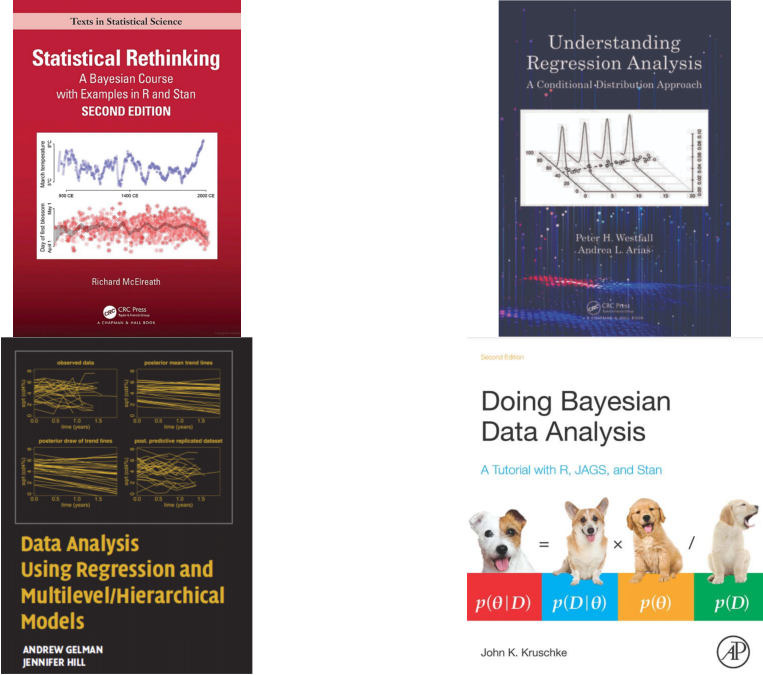
\includegraphics[keepaspectratio]{bookdown-demo_files/figure-latex/unnamed-chunk-1-1.pdf}}

\section{If you need a good reason to buy great books\ldots{}}\label{if-you-need-a-good-reason-to-buy-great-books}

Think of the total costs of your education. You want to extract maximum
benefit from it. In the US, an education costs \href{https://www.finaid.ucsb.edu/docs/default-source/default-document-library/2024-2025-undergrad-coa.pdf?sfvrsn=fb791f8a_4}{a lot}.
In beautiful Switzerland, the \href{https://www.zhaw.ch/de/sml/studium/master/kosten}{tuition fees} (if applicable) are nowhere near these figures.
Costs you could consider are opportunity costs of not working.
A comparison with both, a foreign education or opportunity costs,
justifies the investment in good books.
Or: The costs of all the good books of your education combined are probably less than an iPhone Pro.

\chapter{Introduction}\label{intro}

\section{What is statistical modeling and what do we need this for?}\label{what-is-statistical-modeling-and-what-do-we-need-this-for}

Typically, one simplifies the complex reality (and loses information)
in order to make it better
\textbf{understandable} (explainable), mathematically treatable and to make \textbf{predictions}.

Underlying our models, there are theories which should be \href{https://en.wikipedia.org/wiki/Falsifiability}{falsifiable}
and testable.
For instance, I would be really surprised if I pull up my multimeter and measure the voltage (V) and
electric current (I) at a resistence (R) in a circuit and find that \href{https://en.wikipedia.org/wiki/Ohm\%27s_law}{Ohm's law} \(V = IR\) is not true.
This \href{https://en.wikipedia.org/wiki/Scientific_law}{\textbf{law}}
can be tested over and over again and if one would find a single valid counterexample,
the law would be falsified. It is also true that the law is probably not 100\% accularate,
but an extremely precise approximation of reality. Real-world measurements carry
measurement errors and when plotting the data, one would see that the data points
might not lie exactly on a straight line. This is not a problem.

A \href{https://en.wikipedia.org/wiki/Statistical_model}{statistical model}
is a mathematical framework that represents the
relationships between variables, helping us understand, infer, and
predict patterns in data. It acts as a bridge between observed data
and the real-world processes that generated them. In health research,
where variability and uncertainty are inherent, statistical models are
valuable tools for making sense of complex phenomena.
You can watch \href{https://www.youtube.com/watch?v=3d5ivs_8amQ&ab_channel=VeryNormal}{this} as short intro.

In \href{https://jdegenfellner.github.io/Script_QM1_ZHAW/probs.html}{QM1} we have already
made testable predictions with respect to the probability of an event.
In our 1000-researcher experiment we stated for instance, that the probability of
obeserving \(66\) or more findings would be very unlikely. If such an event would
occur (while not repeating the experiment many times), we would reconsider our model.
Inexactly, we could have stated something like: ``We will not see more than 100 findings by chance.''
With respect to our multiple choice test at the end of QM1 we could predict:
``We will not see a single person answering all questions correctly by chance in our
lifetime (given the frequency of tests).'' Note, that in this context, the word \textbf{predict}
is used with respect to a future event (chance finding or chance passing of the test).
As we will see, there does not necessarily have to be a temporal connection in order
to \emph{predict} something.

Depending on the task at hand, we would use different models.
In any case, logical reasoning and critical thinking comes first,
then comes the model. \textbf{It makes no sense to estimate statistical models just for the sake of it}.

\textbf{All models are wrong, but some are useful}.
Or to quote \href{https://www.tandfonline.com/doi/abs/10.1080/01621459.1976.10480949}{George Box}:

\begin{quote}
``Since all models are wrong the scientist cannot obtain
a `correct' one by excessive elaboration. On the contrary
following William of Occam he should seek an economical
description of natural phenomena. Just as the ability to
devise simple but evocative models is the signature of the
great scientist so overelaboration and overparameterization is often the mark of mediocrity.''
\end{quote}

In my opinion, statistical modeling is an art form: difficult and beautiful.

\textbf{One goal of this course} is to improve interpretation and limitations of statistical models.
They are not magical tools turning data into truth. Firstly, the rule gargabe in, garbage out (GABA) applies.
Secondly, statistical models are based on data and their variability and have inherent limitations
one cannot overcome even with the most sophisticated models. This is expressed for instance
in the so-called \href{https://en.wikipedia.org/wiki/Bias\%E2\%80\%93variance_tradeoff}{bias-variance trade-off}.
You can't have it all.

\subsection{Explanatory vs.~Predictive Models}\label{explanatory-vs.-predictive-models}

I can recommend reading \href{https://projecteuclid.org/journals/statistical-science/volume-25/issue-3/To-Explain-or-to-Predict/10.1214/10-STS330.full}{this}
article by Shmueli et al.~(2010) on this topic.

Statistical models serve different purposes depending on the research question. Two primary goals are \textbf{explanation}
and \textbf{prediction}, and each requires a different approach:

\textbf{Explanatory models (the harder of the two)} focus on understanding causal
relationships.
These models aim to uncover mechanisms and answer \textbf{``why''}
questions. For example:

\begin{itemize}
\tightlist
\item
  Does smoking increase the risk of lung cancer? \textbf{Yes}. (If you want to see what a large effect-size looks like, check out \href{https://bmjopen.bmj.com/content/bmjopen/8/10/e021611.full.pdf}{this study}.)
\item
  How large is the \textbf{effect} (causal) of smoking on lung cancer? \textbf{Large}.
\item
  Does pain education and graded sensorimotor relearning improve disability (a question we ask in
  our \href{https://data.snf.ch/grants/grant/220585}{Resolve Swiss project})?
\end{itemize}

Explanatory models are \textbf{theory-driven}, designed to test hypotheses. Here, one wants to understand the underlying
mechanisms and the relationships between variables and hence often uses (parsimonious) models that are more interpretable,
like linear regression.

\textbf{Predictive models} prioritize forecasting/predicting (future) outcomes based on patterns in the data.
These models aim to answer \textbf{``what will happen?''} For instance:

\begin{itemize}
\tightlist
\item
  \href{https://www.tandfonline.com/doi/abs/10.1080/03091902.2020.1822940}{Gait analysis} using Machine Learning (ML)?
\item
  \href{https://jamanetwork.com/journals/jamadermatology/fullarticle/2756346}{Skin cancer detection} using neural networks?
\item
  If I know the age, sex and weight of a person, can I predict his/her height?
  Can I predict the height better with the given covariates compared to just
  guessing by using the mean height of my sample for the next patient?
\end{itemize}

Predictive models are \textbf{data-driven}, often using complex algorithms to achieve high accuracy.
Their success is measured using metrics like \href{https://computersciencewiki.org/index.php/Root-mean-square_error_(RMSE)}{Root Means Square Error}
(RMSE), \href{https://en.wikipedia.org/wiki/Receiver_operating_characteristic\#:~:text=The\%20area\%20under\%20the\%20curve,ranks\%20higher\%20than\%20'negative'}{Area Unter the Curve}
(AUC), or \textbf{prediction error on new, unseen data}.
Any amount of model complexity is allowed. One could for instance estimate a
\href{https://en.wikipedia.org/wiki/Neural_network_(machine_learning)}{neural network} (``just'' another statistical model)
with many hidden layers and neurons in order to improve prediction quality. Interpretability of the model weights is not a priority here.

While explanatory and predictive goals often complement each other,
their differences highlight the importance of clearly defining the purpose
of your analysis. In applied health research, explanatory models help identify
causal mechanisms, while predictive models can guide real-world decisions by
providing actionable forecasts. Together, they enhance both our understanding
of phenomena and our ability to make informed decisions in complex environments.

\subsection{Individual vs.~Population Prediction}\label{individual-vs.-population-prediction}

Another important distinction is between \textbf{individual vs.~population} prediction.
In the smoking example above, we can be very sure about the mean effects that smoking has on lung cancer.
On an individual level, it is \href{https://www.liebertpub.com/doi/10.1089/rej.2019.2298}{harder to predict the outcome}.
Nevertheless, individual predictions will be (notably) better than random guessing. We will discuss this in greater detail.

Statistical models are often much worse than one would naively expect, but
they very often better than experts. If you are interested and want to
boost your confidence in the predictive ability of statistical models,
I recommend reading chapter 21 (``Intuitions vs.~Formulas'') of Daniel Kahneman's book
\href{https://en.wikipedia.org/wiki/Thinking,_Fast_and_Slow}{``Thinking, Fast and Slow''}
(available in the ZHAW library).

\subsection{Practical Use of Statistical Models}\label{practical-use-of-statistical-models}

In my optinion, we should never be afraid to test our statistical models (as honestly as possible) against reality.
We could for instance ask ourselves:

\begin{itemize}
\item
  ``How much better does this model estimate an outcome than the arithmetic mean?
  (i.e., the linear model with just an intercept)''
\item
  ``How much better does this model classify than random guessing?''
\item
  Is it worth the effort to collect data and estimate this model by using hundreds of hours of our time?
\end{itemize}

In some cases, these questions can be answered straightforwardly.

\begin{itemize}
\item
  In advertising (Google, Facebook, \ldots), a couple of percentage points in prediction quality might make a difference of millions
  of dollars in revenue offsetting the statistitians salary by a large margin.
\item
  Improved forecasts of a few percentage points in the stock market or just being \href{https://en.wikipedia.org/wiki/Jim_Simons}{slightly better}
  than the average, will make you faboulously rich.
\item
  Improved cancer forecasting might save lives, money and pain and is of course
  not only measured in financial gains.
\end{itemize}

\subsection{Start at the beginning}\label{start-at-the-beginning}

What do we actually want to do in general? Very broadly speaking we want to:
\textbf{describe} the association of variables to each other that carry variability.
Hence, the relationship is not deterministic like \[y = 2x + 3\] but rather we need
to ``loosen up'' the relationship to account for variability (in \(x\) and \(y\)).
So, \(y\) and \(x\) are not fixed but aflicted with uncertainty.
Depending on your philosophical view, you might say you want to find
the ``true'' but unknown relationship (here, \(2\) and \(3\) are the true coefficients) between variables.
This is what we do in simulation studies all the time: We know the true relationship,
simulate data by adding variability and then try to estimate the true relationship we assumed in the first place.
This is an \textbf{advantage} the pioneers of statistics did not have. We can simulate
millions of lines of data at the click of a button.
For some practical applications, we can get a really nice and complete answer to our question
(for instance sample size for proportions).

So we are looking for a function \(f\) such that

\[ \mathbf{Y} = f(\mathbf{X}) \]

where

\begin{itemize}
\tightlist
\item
  \(\mathbf{Y}\) is the ``outcome'', ``dependent variable'' or ``response''.
\item
  \(\mathbf{X}\) are the ``predictors''. \(\mathbf{X}\) can be a single Variable \(x\) or many
  variables \(x_1, x_2, \ldots, x_p\).
\end{itemize}

It is important to be aware of the notation here:
``Predict'' does \textbf{not necessarily} mean that we can predict the value in
the future. It merely means we estimate the value (or mean) of \(Y\) given \(X\).

\begin{itemize}
\tightlist
\item
  This can be done at the same time points, known as \textbf{cross-sectional} analysis (``What is the maximum jumping height
  of a person given their age at a certain point in time, whereas both variables are measured at the same time?'');
\item
  or at different time points, known as \textbf{longitudinal analysis} (``What is the maximum jumping height of a person 10 years later (\(t_2\))
  given their baseline health status at time \(t_1\)?'').
\end{itemize}

The \textbf{simplest statistical model} would be the \textbf{mean model} where \(Y\) is ``predicted'' by a
constant: \(Y = c\) which (at least in the classical linear regression) turns out to be \(c = \bar{x}\).
This simple model is often surprisingly good, or, to put it in other words, models with more complexity
are often not that much better.

\section{A (simple) model for adult body heights in the Bayesian framework}\label{a-simple-model-for-adult-body-heights-in-the-bayesian-framework}

As repetition, read the parts about \href{https://jdegenfellner.github.io/Script_QM1_ZHAW/bayes_statistics.html}{Bayes statistics from QM1}
again to refresh your memory about the Bayesian framework.

It's recommendable to read the beginning of the book \href{https://civil.colorado.edu/~balajir/CVEN6833/bayes-resources/RM-StatRethink-Bayes.pdf}{Statistical rethinking}
(hint: the online-version of the book differs a bit from the paper-version)
up until page 39 as well. We are not completely new to the topic of Bayes thanks
to QM1. In the Bayesian setting we use (well argued for) prior knowledge about a
parameter or effect and update this knowledge with new data.

We want to \textbf{start building our first model} right away.

Let's begin with the example in
\href{https://civil.colorado.edu/~balajir/CVEN6833/bayes-resources/RM-StatRethink-Bayes.pdf}{Statistical rethinking}
using data from the \href{https://en.wikipedia.org/wiki/\%C7\%83Kung_people}{!Kung San}
people.

\begin{Shaded}
\begin{Highlighting}[]
\FunctionTok{library}\NormalTok{(rethinking)}
\FunctionTok{data}\NormalTok{(}\StringTok{"Howell1"}\NormalTok{)}
\NormalTok{d }\OtherTok{\textless{}{-}}\NormalTok{ Howell1}
\FunctionTok{str}\NormalTok{(d)}
\end{Highlighting}
\end{Shaded}

\begin{verbatim}
## 'data.frame':    544 obs. of  4 variables:
##  $ height: num  152 140 137 157 145 ...
##  $ weight: num  47.8 36.5 31.9 53 41.3 ...
##  $ age   : num  63 63 65 41 51 35 32 27 19 54 ...
##  $ male  : int  1 0 0 1 0 1 0 1 0 1 ...
\end{verbatim}

\begin{Shaded}
\begin{Highlighting}[]
\NormalTok{d2 }\OtherTok{\textless{}{-}}\NormalTok{ d[d}\SpecialCharTok{$}\NormalTok{age }\SpecialCharTok{\textgreater{}=} \DecValTok{18}\NormalTok{, ] }\CommentTok{\# only adults}
\end{Highlighting}
\end{Shaded}

We want to model the adult height of the !Kun San people
using prior knowledge (about the Swiss population) and data.

\begin{Shaded}
\begin{Highlighting}[]
\FunctionTok{library}\NormalTok{(tidyverse)}
\NormalTok{d2 }\SpecialCharTok{\%\textgreater{}\%} \FunctionTok{ggplot}\NormalTok{(}\FunctionTok{aes}\NormalTok{(}\AttributeTok{x =}\NormalTok{ height)) }\SpecialCharTok{+} \FunctionTok{geom\_histogram}\NormalTok{()}
\end{Highlighting}
\end{Shaded}

\pandocbounded{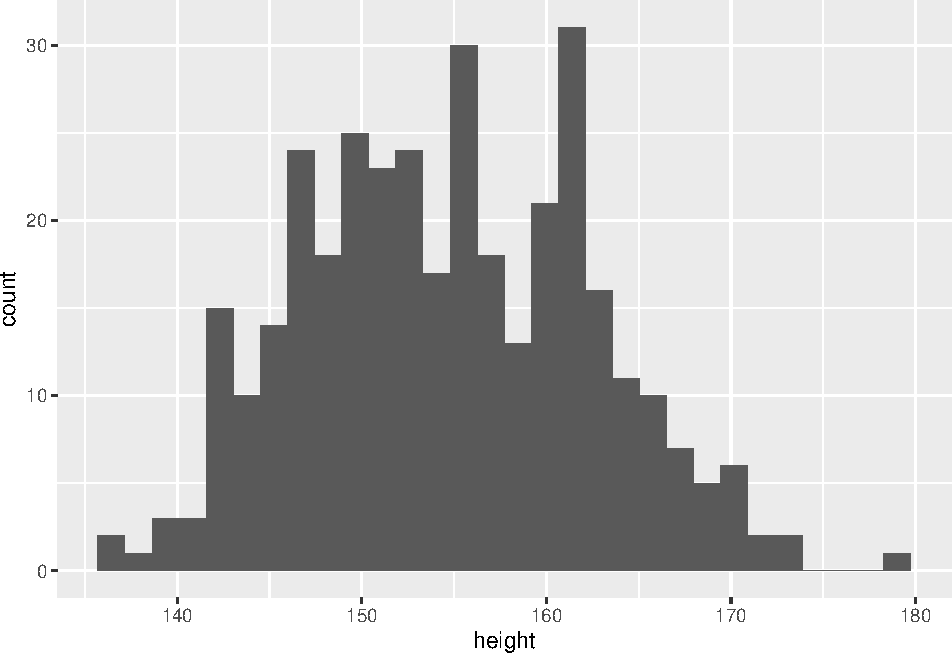
\includegraphics[keepaspectratio]{bookdown-demo_files/figure-latex/unnamed-chunk-3-1.pdf}}

Since we already have domain knowledge in this area, we can say that heights are usually normally distributed,
or at least a mixture of normal distrubutions (female/male).
We assume the following model:
\[h_i \sim \text{Normal}(\mu, \sigma)\]

As in \href{https://jdegenfellner.github.io/Script_QM1_ZHAW/}{QM1},
we want to start with a Bayesian model and hence, we need some priors.

Since we are in Switzerland and just for fun, we use the mean of
\href{https://www.bfs.admin.ch/asset/de/30305714}{Swiss body heights}
as expected value for the \textbf{prior for the mean}.
According to the link (Bundesamt für Statistik),
the mean height of \(n=21,873\) people in the Swiss sample is
\(171.1\) cm. We choose the same \(\sigma\) for the prior of the normal
as in the book not to deviate too much from the example at hand.

Next comes our \textbf{model definition in the Bayesian framework}, which
I often find more intuitive than the Frequentist approach:

\[
h_i \sim \text{Normal}(\mu, \sigma)
\]
\[
\mu \sim \text{Normal}(171.1, 20)
\]
\[
\sigma \sim \text{Uniform}(0, 50)
\]

\textbf{Description of the model definition}: The heights are normally distributed with unknown mean and
standard deviation. As our current knowledge about the mean height, we use
a prior distribution for the mean (we do not know but want to estimate) by
assuming the mean of a population we know and a standard deviation of \(20\) cm which
allows are rather large range of possible values for \(\mu\)
(the unobserved population mean of the !Kung San people).
\(\sigma\) (the unobserved standard deviation of the population of !Kun San people)
is also unknown and a priori we restrict ourselves to values
between \(0\) and \(50\) cm, whereas we assign equal plausibility to all
values in this range (which can and should be critically discussed).

\textbf{Vizualisation of the model structure}:
\pandocbounded{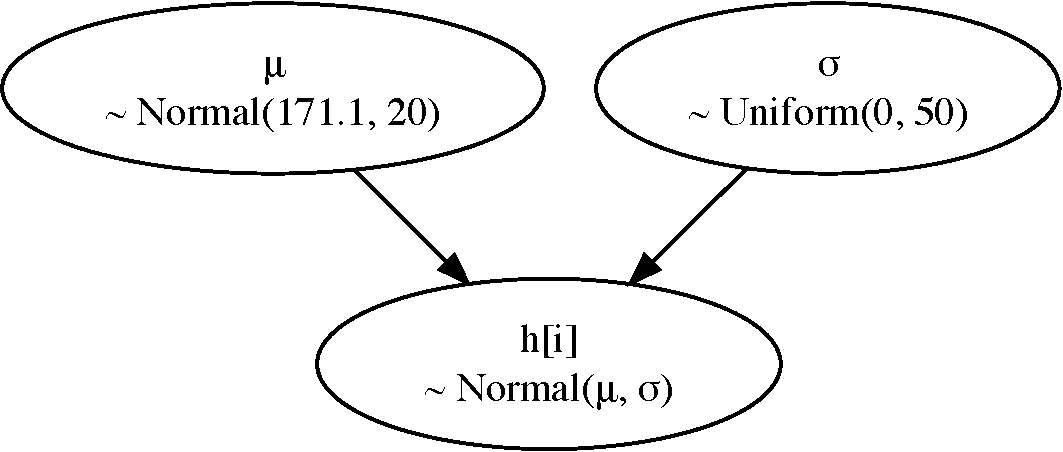
\includegraphics[keepaspectratio]{bookdown-demo_files/figure-latex/unnamed-chunk-4-1.pdf}}

Mind that there is a \textbf{conceptual difference} between the normal distribution of the heights
and the normal prior distribution of the mean. The latter expresses our prior knowledge/insecurity
about the unobserved mean of the normal distribution of the heights. The normal distribution of the heights says we expect the heights to be normally distributed
but we do not know the parameters (\(\mu\) and \(\sigma\)) yet. We will
estimate these parameters using prior knowledge and the data.

Of course we would not need the prior here due to the large sample size,
but let's do it anyways for demonstration purposes.
We are not completely uninformed about body heights and express our
knowledge with the prior for \(\mu\).
The \(20\) in the prior for the mean expresses our range of possible true
mean values and aknowledge
that there are a variety of different subpopulations with different means.

Using the Swiss data in the \href{https://www.bfs.admin.ch/asset/de/30305714}{link}
one could estimate that the standard deviation of the heights
from \(21,873\) Swiss people is around is \(25.67\) cm (\hyperref[exercise1_Intro]{Exercise 1}).

Remember, in the Baysian world, there is no \textbf{fixed but unknown}
parameter, but instead we define a distribution over the unobserved parameter.

We \textbf{visualize the prior for \(\mu\)}:

\begin{Shaded}
\begin{Highlighting}[]
\FunctionTok{curve}\NormalTok{(}\FunctionTok{dnorm}\NormalTok{(x, }\FloatTok{171.1}\NormalTok{, }\DecValTok{20}\NormalTok{), }\AttributeTok{from =} \DecValTok{100}\NormalTok{, }\AttributeTok{to =} \DecValTok{250}\NormalTok{)}
\end{Highlighting}
\end{Shaded}

\pandocbounded{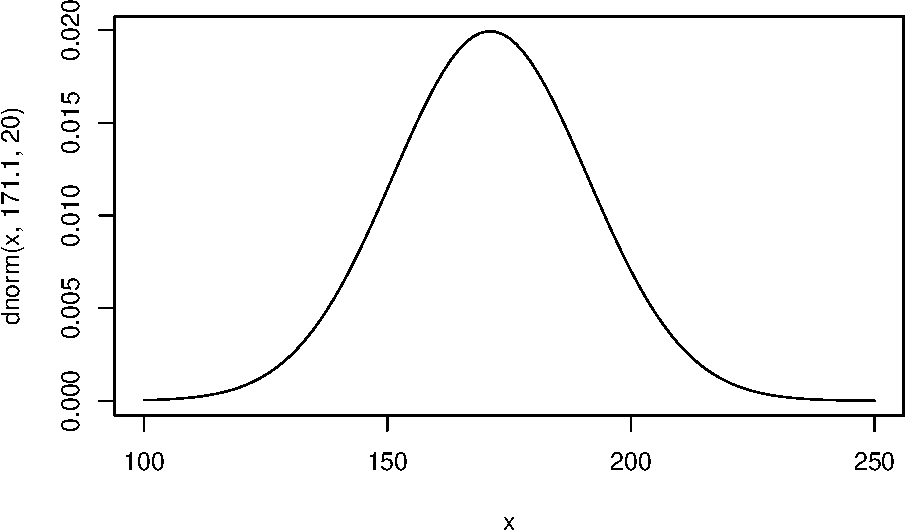
\includegraphics[keepaspectratio]{bookdown-demo_files/figure-latex/unnamed-chunk-5-1.pdf}}

A wide range of population means is possible. Once could discuss this distribution
and maybe further restrict it.

The \textbf{prior for \(\sigma\)} is uniform between \(0\) and \(50\) cm. This is a very wide prior and
just constrains the values to be positive and below \(50\) cm.
This could be stronger of course.

\textbf{Visualization of the prior for \(\sigma\)}:

\begin{Shaded}
\begin{Highlighting}[]
\FunctionTok{curve}\NormalTok{(}\FunctionTok{dunif}\NormalTok{(x, }\DecValTok{0}\NormalTok{, }\DecValTok{50}\NormalTok{), }\AttributeTok{from =} \SpecialCharTok{{-}}\DecValTok{10}\NormalTok{, }\AttributeTok{to =} \DecValTok{60}\NormalTok{)}
\end{Highlighting}
\end{Shaded}

\pandocbounded{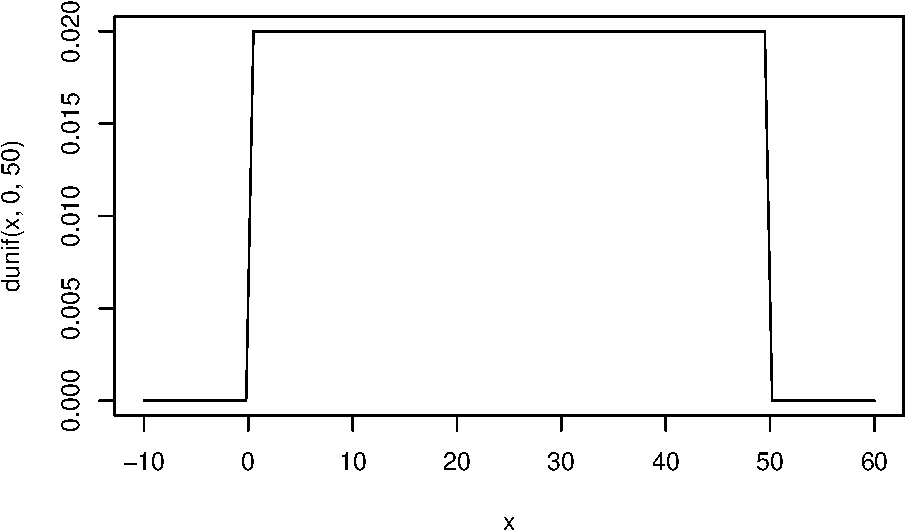
\includegraphics[keepaspectratio]{bookdown-demo_files/figure-latex/unnamed-chunk-6-1.pdf}}

Note, we didn't specify a prior probability distribution of heights
directly, but once we've chosen priors for \(\mu\) and \(\sigma\), these imply a
prior distribution of individual heights.

\textbf{Without} even having seen the \textbf{new data}, we can check what our prior
(model) for heights would predict. This is important. If the prior already
predicts impossible values, we should reconsider our priors and/or model.

So, we simply draw \(\mu\) and \(\sigma\) from the priors and then draw heights
from the normal distribution using the drawn parameters.

\textbf{Vizualisation of the prior for heights}:

\begin{Shaded}
\begin{Highlighting}[]
\NormalTok{sample\_mu }\OtherTok{\textless{}{-}} \FunctionTok{rnorm}\NormalTok{(}\DecValTok{10}\SpecialCharTok{\^{}}\DecValTok{4}\NormalTok{, }\FloatTok{171.1}\NormalTok{, }\DecValTok{20}\NormalTok{)}
\NormalTok{sample\_sigma }\OtherTok{\textless{}{-}} \FunctionTok{runif}\NormalTok{(}\DecValTok{10}\SpecialCharTok{\^{}}\DecValTok{4}\NormalTok{, }\DecValTok{0}\NormalTok{, }\DecValTok{50}\NormalTok{)}
\NormalTok{prior\_h }\OtherTok{\textless{}{-}} \FunctionTok{rnorm}\NormalTok{(}\DecValTok{10}\SpecialCharTok{\^{}}\DecValTok{4}\NormalTok{, sample\_mu, sample\_sigma)}
\FunctionTok{length}\NormalTok{(prior\_h)}
\end{Highlighting}
\end{Shaded}

\begin{verbatim}
## [1] 10000
\end{verbatim}

\begin{Shaded}
\begin{Highlighting}[]
\FunctionTok{dens}\NormalTok{(prior\_h)}
\end{Highlighting}
\end{Shaded}

\pandocbounded{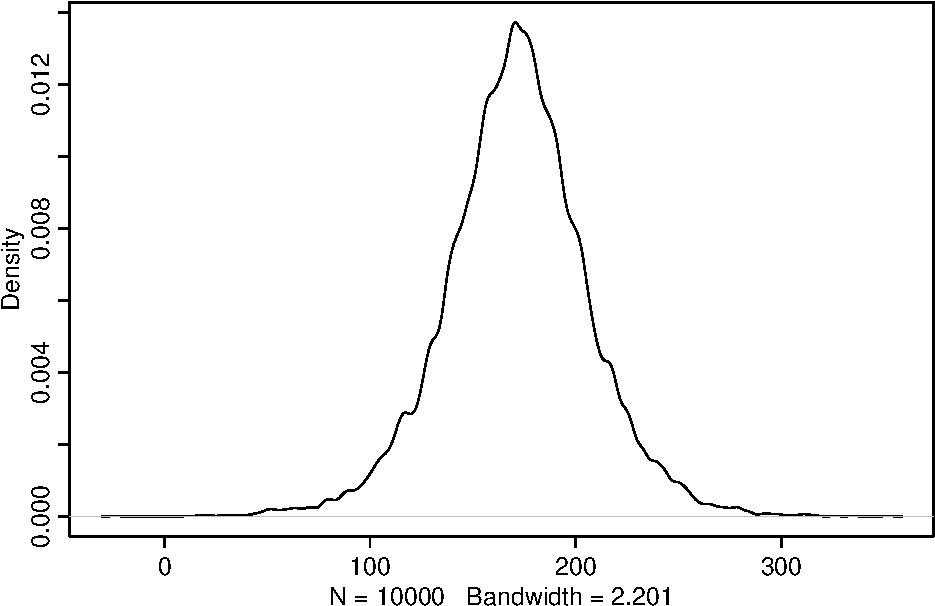
\includegraphics[keepaspectratio]{bookdown-demo_files/figure-latex/unnamed-chunk-7-1.pdf}}

The prior is not itself a Gaussian distribution, but a distribution of
relative plausibilities of different heights, \textbf{before} seeing the data.

Note how we have created the model predictions for heights.
We first drew \(\mu\) and \(\sigma\) independently
(there is no arrow between \(\mu\) and \(\sigma\)) from the priors.
Then we drew heights from the normal distribution using the drawn parameters.
You just follow the model structure.

Now, there are a couple of different ways to estimtate the model incorporating
the new data. For didactic reasons, grid approximation is often used (as in the books).
For many parameters, this approach becomes more and more infeasible (due to combinatorial explosion).

We will skip that for now and use quadratic approximation instead which
works well for many common procedures in applied statistics (like linear regression).
Later, you'll probably use (or the software in the background) mostly Markov
chain Monte Carlo (MCMC) sampling to get the posterior.
\href{https://civil.colorado.edu/~balajir/CVEN6833/bayes-resources/RM-StatRethink-Bayes.pdf}{Pages 39 and the following}
explain the 3 concepts grid approximation, quadratic approximation and MCMC.

In short, \textbf{quadratic approximation} assumes that our posterior distribution
of body heights can be approximated well by a normal distribution,
at least near the peak.

Please read the \hyperref[bivariate_normal]{addendum} to get a clearer picture of
what a bivariate normal distribution is.

Using the \texttt{rethinking} package we can estimate the model using quadratic approximation.
First, we define the model in the \texttt{rethinking} syntax (see R code 4.25 in the book).

\begin{Shaded}
\begin{Highlighting}[]
\FunctionTok{library}\NormalTok{(rethinking)}
\NormalTok{flist }\OtherTok{\textless{}{-}} \FunctionTok{alist}\NormalTok{(}
\NormalTok{  height }\SpecialCharTok{\textasciitilde{}} \FunctionTok{dnorm}\NormalTok{(mu, sigma),}
\NormalTok{  mu }\SpecialCharTok{\textasciitilde{}} \FunctionTok{dnorm}\NormalTok{(}\FloatTok{171.1}\NormalTok{, }\DecValTok{20}\NormalTok{),}
\NormalTok{  sigma }\SpecialCharTok{\textasciitilde{}} \FunctionTok{dunif}\NormalTok{(}\DecValTok{0}\NormalTok{, }\DecValTok{50}\NormalTok{)}
\NormalTok{)}
\end{Highlighting}
\end{Shaded}

Then we estimate/fit the model using quadratic approximation.

\begin{Shaded}
\begin{Highlighting}[]
\NormalTok{m\_heights }\OtherTok{\textless{}{-}} \FunctionTok{quap}\NormalTok{(flist, }\AttributeTok{data =}\NormalTok{ d2)}
\end{Highlighting}
\end{Shaded}

Now let's take a look at the fitted model:
(Note: In the online-version of the book, they used the command \texttt{map} instead of \texttt{quap}.)

The \texttt{precis}function displays concise parameter estimate information
(from the posterior) for an existing model fit.

\begin{Shaded}
\begin{Highlighting}[]
\FunctionTok{precis}\NormalTok{(m\_heights)}
\end{Highlighting}
\end{Shaded}

\begin{verbatim}
##             mean        sd       5.5%      94.5%
## mu    154.604096 0.4119939 153.945650 155.262542
## sigma   7.731326 0.2913853   7.265636   8.197016
\end{verbatim}

Above, we see the mean of the posterior for \(\mu\) \textbf{and} \(\sigma\);
and a \textbf{89\% credible interval} for those parameters.
Note that these are rather tight credible intervals. We are rather confident that the mean is somewhere between
\(154\) and \(155\) cm and the standard deviation is between \(7\) and \(8\) cm.

We can now plot the posterior distribution of the mean (\(\mu\)) and the standard
deviation (\(\sigma\)) separately by drawing from the posterior distribution.

\begin{Shaded}
\begin{Highlighting}[]
\NormalTok{post }\OtherTok{\textless{}{-}} \FunctionTok{extract.samples}\NormalTok{(m\_heights, }\AttributeTok{n =} \DecValTok{10}\SpecialCharTok{\^{}}\DecValTok{4}\NormalTok{)}
\FunctionTok{head}\NormalTok{(post)}
\end{Highlighting}
\end{Shaded}

\begin{verbatim}
##         mu    sigma
## 1 154.5537 7.888043
## 2 154.1767 7.757970
## 3 154.6272 7.267756
## 4 154.6688 7.800767
## 5 154.9711 7.930193
## 6 154.3454 7.876730
\end{verbatim}

\begin{Shaded}
\begin{Highlighting}[]
\FunctionTok{dens}\NormalTok{(post}\SpecialCharTok{$}\NormalTok{mu)}
\end{Highlighting}
\end{Shaded}

\pandocbounded{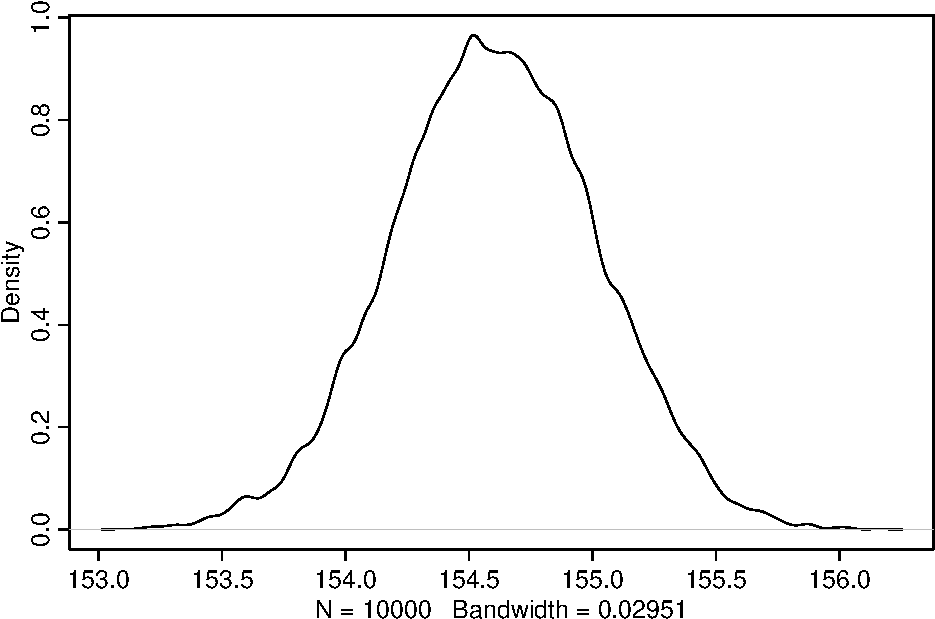
\includegraphics[keepaspectratio]{bookdown-demo_files/figure-latex/unnamed-chunk-11-1.pdf}}

\begin{Shaded}
\begin{Highlighting}[]
\FunctionTok{dens}\NormalTok{(post}\SpecialCharTok{$}\NormalTok{sigma)}
\end{Highlighting}
\end{Shaded}

\pandocbounded{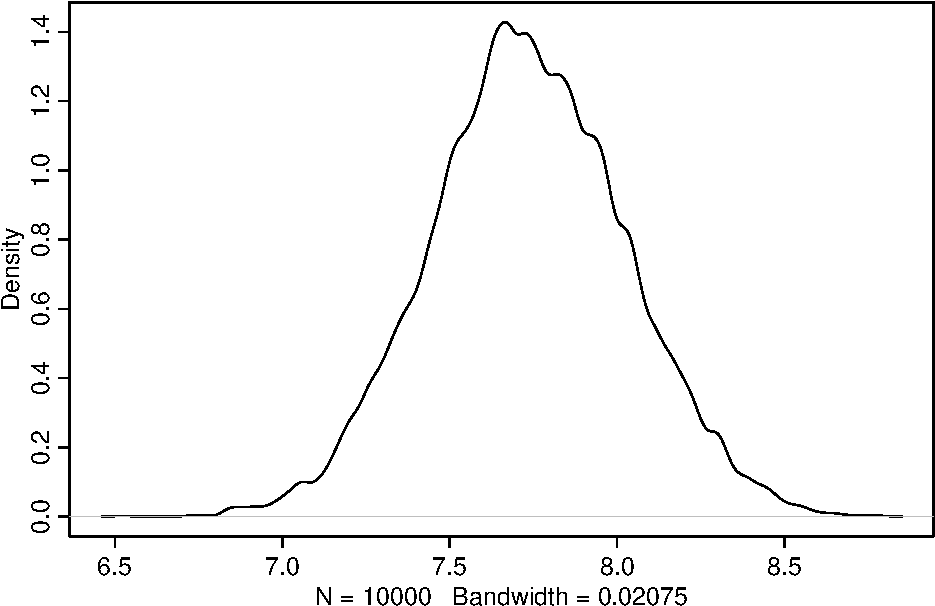
\includegraphics[keepaspectratio]{bookdown-demo_files/figure-latex/unnamed-chunk-11-2.pdf}}

Note, that \textbf{these samples come from a multi-dimensional posterior distribution}.
In our case, we approximated the \textbf{joint} posterior distribution of \(\mu\) \emph{and} \(\sigma\) with a
\href{https://en.wikipedia.org/wiki/Multivariate_normal_distribution}{bivariate normal distribution}.
They are not necessarily independent from each other, but in this case they are (see \hyperref[exercise6_Intro]{exercise 6}).
We know this from the prior definition above. \(\mu\) and \(\sigma\) are both
defined as normal respectively uniform distributions and by definition do not
influence each other. This is also visible in the vizualisation of the model structure:
There is no confounding variable or connection between those priors. One could
think of a common variable \(Z\) that influences both \(\mu\) and \(\sigma\). This could
be genetic similarity which could influence both \(\mu\) and \(\sigma\).

Let's verify that \(\mu\) and \(\sigma\) are uncorrelated:

\begin{Shaded}
\begin{Highlighting}[]
\FunctionTok{vcov}\NormalTok{(m\_heights)}
\end{Highlighting}
\end{Shaded}

\begin{verbatim}
##               mu      sigma
## mu    0.16973901 0.00015376
## sigma 0.00015376 0.08490540
\end{verbatim}

gives you the variance-covariance matrix of the parameters of the posterior
distribution. In the diagonal you see the variance of the parameters.

\begin{Shaded}
\begin{Highlighting}[]
\FunctionTok{diag}\NormalTok{(}\FunctionTok{vcov}\NormalTok{(m\_heights))}
\end{Highlighting}
\end{Shaded}

\begin{verbatim}
##        mu     sigma 
## 0.1697390 0.0849054
\end{verbatim}

And we can compute the correlation matrix easily:

\begin{Shaded}
\begin{Highlighting}[]
\FunctionTok{cov2cor}\NormalTok{(}\FunctionTok{vcov}\NormalTok{(m\_heights))}
\end{Highlighting}
\end{Shaded}

\begin{verbatim}
##                mu       sigma
## mu    1.000000000 0.001280811
## sigma 0.001280811 1.000000000
\end{verbatim}

Let's plot the posterior in 3D, because we \textbf{can}:

\pandocbounded{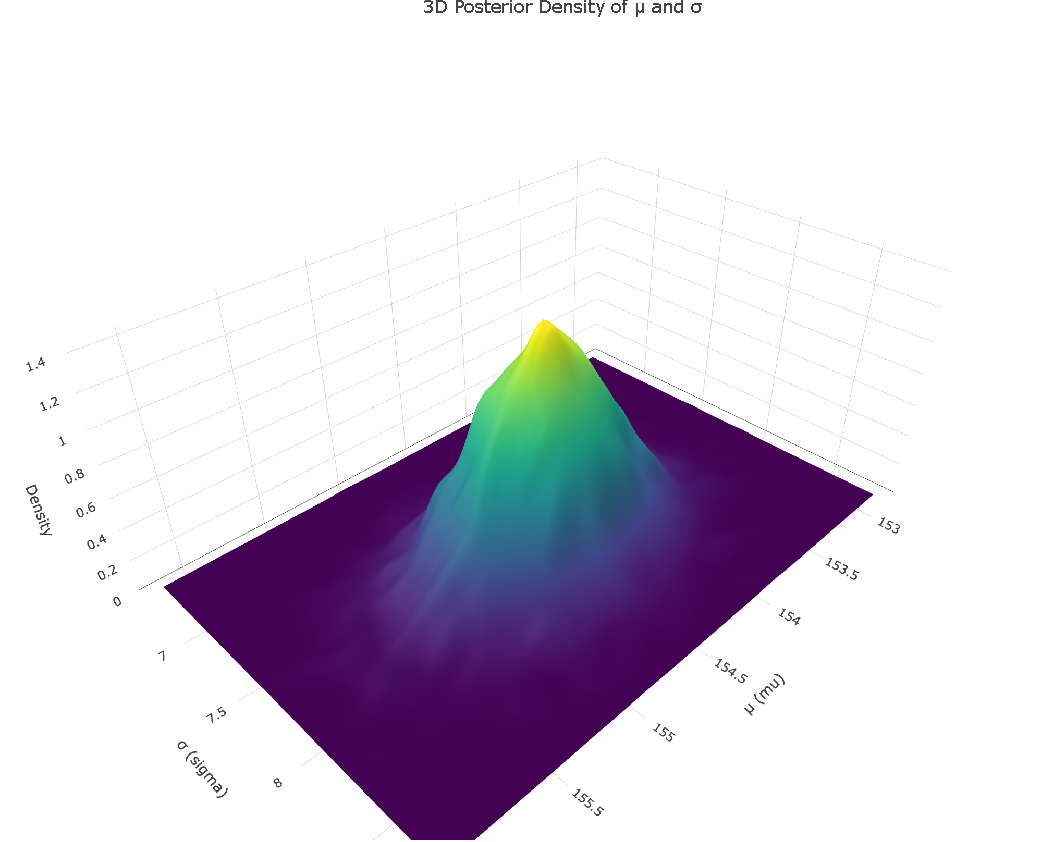
\includegraphics[keepaspectratio]{bookdown-demo_files/figure-latex/posterior-3d-correct-1.pdf}}

\textbf{How beautiful ist that?}

This shows how credible each combination of \(\mu\) and \(\sigma\) is based on our priors and the data observed.
The higher the mountain for a certain parameter combination, the more credible this combination is.

We see in the 3D plot, that the ``mountain'' is not rotated, indicating
graphically that the parameters are independent from each other.

We also see in the correlation matrix, the correlation of the parameters is \(\sim 0\).
In the \href{https://en.wikipedia.org/wiki/Correlation\#Correlation_and_independence}{context of a joint normal distribution},
this means that the parameters are also independent.

And, it is not an accident that the posterior looks like this. Using quadratic approximation,
we used the bivariate normal distribution to \textbf{approximate} the posterior.

\section{Classical approach for the simplest model}\label{classical_simple_mean_model}

We have seen, how we could use prior knowledge to fit a very simple model
for body heights of a population (!Kung San) in the Bayesian framework.

Now, let's start at the same point in the classical framework.
Here, we do not use any prior knowledge, at least not that explicitely.

The classical approach to fit a regression line is the so-called
\textbf{\href{https://en.wikipedia.org/wiki/Least_squares}{least squares method}}.

There are hundreds of \href{https://www.youtube.com/results?search_query=linear+regression}{videos online}
explaining this method in great detail
with animations. Maybe watch these videos later, when we add a predictor to the mean model,
since most of instructional videos start at the simple linear regression using
two parameters (intercept (\(\beta_0\) or \(\alpha\)) and slope (\(\beta_1\))).

The \textbf{(simple mean-) model} is:

\[ Y_i = height_i = c + \varepsilon_i \]

\begin{itemize}
\tightlist
\item
  for some \(c \in \mathbb{R}\) and
\item
  normally distributed errors \(\varepsilon_i \sim \text{Normal}(0, \sigma)\).
\end{itemize}

The errors \(\varepsilon_i\) are on average zero and have a constant standard deviation of \(\sigma\).
So, we assume there is a fixed, but unknown, constant \(c\) that we want to estimate and we
assume that there is a special sort of error in our model that is normally distributed.
Sometimes there is a large deviation from the true \(c\), sometimes there is a small deviation.
On average, the deviations are zero and the \textbf{errors should also be independent from each other}:
\[ \varepsilon_i \perp \varepsilon_j \text{ for } i \neq j\]
This means that just because I have just observed a large deviation from the true \(c\)
does not mean, that the probability of a large deviation in the next observation is higher/lower.
Note, that we cannot readily define different types of errors in the classical framework.

But what is \(c\)? We determine the shape of the model
ourselves (constant model, or mean model) and then estimate the parameter \(c\).
By defining the shape of the model ourselves and imposing a distribution where we want to
estimate the parameter of said distribution, we are in \textbf{parametric statistics}.

We choose the \(c\) which minimizes the sum of squared errors from the actual heights.
This has the advantage that deviations upper and lower from the actual height are
equally weighted. The larger the deviation the (quadratically) larger the penalty.

\textbf{Why do we do that?} Because, if the model assumptions (more on that later)
are correct, the least squares
estimator is a really good estimator. How good? Later\ldots{}

We want to miminize the following function:

\[ SSE \text{ (Sum of Squared Errors) }(c) = (height_1 - c)^2 + (height_2 - c)^2 + 
\ldots + (height_n - c)^2 =\]
\[ = \sum_{i=1}^{n} (height_i - c)^2\]

The SSE is a function of \(c\) and we want to find the \(c\) that minimizes the function.
Since it is a quadratic function, we can always find the minimum.
We have learnt in school how to do this (hopefully): Take the derivative of the function
and set it to zero. Solve for \(c\) and you have the \(c\) which yields the minimum of SSE(c).

Let's do that:

\[ \frac{d}{dc} SSE(c) =  2(height_1 - c)(-1) + 2(height_2 - c)(-1) + 
\ldots + 2(height_n - c)(-1) =\]
\[ = -2 \sum_{i=1}^{n} (height_i - c)\]

This should be zero for the minimum:
\[ -2 \sum_{i=1}^{n} (height_i - c) = 0\]
\[ \sum_{i=1}^{n} (height_i - c) = 0\]
\[ \sum_{i=1}^{n} height_i - n \cdot c = 0\]
\[ \hat{c} = \frac{1}{n} \sum_{i=1}^{n} height_i = \overline{height_i}\]

The hat over the \(c\) indicates that this is the estimated value of the
true but unknown \(c\).
Everytime we estimate a parameter, we put a hat over it.

And voilà, we have estimated the parameter \(c\) of the model, which is just the
sample mean of all the heights. In contrast to before, we did not put
in a lot of prior knowledge, but just estimated the parameter from the data.

In R, we can do this easily:

\begin{Shaded}
\begin{Highlighting}[]
\NormalTok{mod }\OtherTok{\textless{}{-}} \FunctionTok{lm}\NormalTok{(height }\SpecialCharTok{\textasciitilde{}} \DecValTok{1}\NormalTok{, }\AttributeTok{data =}\NormalTok{ d2)}
\FunctionTok{summary}\NormalTok{(mod)}
\end{Highlighting}
\end{Shaded}

\begin{verbatim}
## 
## Call:
## lm(formula = height ~ 1, data = d2)
## 
## Residuals:
##      Min       1Q   Median       3Q      Max 
## -18.0721  -6.0071  -0.2921   6.0579  24.4729 
## 
## Coefficients:
##             Estimate Std. Error t value Pr(>|t|)    
## (Intercept) 154.5971     0.4127   374.6   <2e-16 ***
## ---
## Signif. codes:  0 '***' 0.001 '**' 0.01 '*' 0.05 '.' 0.1 ' ' 1
## 
## Residual standard error: 7.742 on 351 degrees of freedom
\end{verbatim}

\begin{Shaded}
\begin{Highlighting}[]
\FunctionTok{dim}\NormalTok{(d2)}
\end{Highlighting}
\end{Shaded}

\begin{verbatim}
## [1] 352   4
\end{verbatim}

\begin{Shaded}
\begin{Highlighting}[]
\FunctionTok{mean}\NormalTok{(d2}\SpecialCharTok{$}\NormalTok{height) }\CommentTok{\# same as the intercept}
\end{Highlighting}
\end{Shaded}

\begin{verbatim}
## [1] 154.5971
\end{verbatim}

\begin{Shaded}
\begin{Highlighting}[]
\FunctionTok{sd}\NormalTok{(d2}\SpecialCharTok{$}\NormalTok{height) }\SpecialCharTok{/} \FunctionTok{sqrt}\NormalTok{(}\FunctionTok{nrow}\NormalTok{(d2)) }\CommentTok{\# standard error of the estimator}
\end{Highlighting}
\end{Shaded}

\begin{verbatim}
## [1] 0.4126677
\end{verbatim}

\begin{Shaded}
\begin{Highlighting}[]
\CommentTok{\# test{-}statistic for the intercept:}
\FunctionTok{mean}\NormalTok{(d2}\SpecialCharTok{$}\NormalTok{height) }\SpecialCharTok{/}\NormalTok{ (}\FunctionTok{sd}\NormalTok{(d2}\SpecialCharTok{$}\NormalTok{height) }\SpecialCharTok{/} \FunctionTok{sqrt}\NormalTok{(}\FunctionTok{nrow}\NormalTok{(d2)))}
\end{Highlighting}
\end{Shaded}

\begin{verbatim}
## [1] 374.6285
\end{verbatim}

\begin{Shaded}
\begin{Highlighting}[]
\CommentTok{\# residual standard error:}
\FunctionTok{sqrt}\NormalTok{(}\FunctionTok{sum}\NormalTok{(mod}\SpecialCharTok{$}\NormalTok{residuals}\SpecialCharTok{\^{}}\DecValTok{2}\NormalTok{) }\SpecialCharTok{/}\NormalTok{ (}\FunctionTok{nrow}\NormalTok{(d2) }\SpecialCharTok{{-}} \DecValTok{1}\NormalTok{))}
\end{Highlighting}
\end{Shaded}

\begin{verbatim}
## [1] 7.742332
\end{verbatim}

The \texttt{\textasciitilde{}1} means that there is just a so-called \textbf{intercept} in the model.
There are \textbf{no covariates}, just the constant \(c\).
This is the simplest we can do. \texttt{lm} stands for linear model and with this base
command in R we ask the software to do the least squares estimation for us.

Let's look at the \textbf{R-output} of the model estimation:

\begin{itemize}
\tightlist
\item
  \texttt{lm(formula\ =\ height\ \textasciitilde{}\ 1,\ data\ =\ d2)}: This is the model we estimated.
\item
  \texttt{Residuals}: The difference between the actual height and the estimated height:
  \(r_i = height_i - \hat{c}\). A univariate 5-point summary is given.
\item
  \texttt{Coefficients}: The estimated coefficients of the model. In this case, there is just the intercept.
  We get the

  \begin{itemize}
  \tightlist
  \item
    \texttt{Std.\ Error} of the estimate, i.e.~the \href{https://en.wikipedia.org/wiki/Standard_error}{standard error (SE)} of the mean,
    which is (according to the Central Limit Theorem)
    \[\frac{\sigma}{\sqrt{n}}\] and can be estimated by the sample
    standard deviation divided by the square root of the sample size.
    \(\hat{SE} = \frac{s}{\sqrt{n}}\)
  \item
    the \texttt{t\ value} and the \texttt{Pr(\textgreater{}\textbar{}t\textbar{})} which is the \(p\)-value of the (Wald-)test of
    the null hypothesis that the
    coefficient is zero (\(H_0: \text{intercept}=0\)).
    This is a perfect example of an absolutely useless \(t\)-test.
    Why? Because obviously (\hyperref[exercise2_Intro]{exercise 2}) the population mean of body heights is not zero.
  \end{itemize}
\item
  \texttt{Residual\ standard\ error}: The standard deviation of the residuals \(r_i = height_i - \hat{c}\).
  In this case identical with the sample standard deviation
  of heights (\hyperref[exercise3_Intro]{exercise 3}). \(351\) degrees of freedom. There are \(352\) observations and
  \(1\) parameter estimated (intercept/mean). Hence, there are \(352-1=351\)
  freely movable variables in the statistic of the sample standard deviation.
\end{itemize}

Let's look at the situation graphically:

\pandocbounded{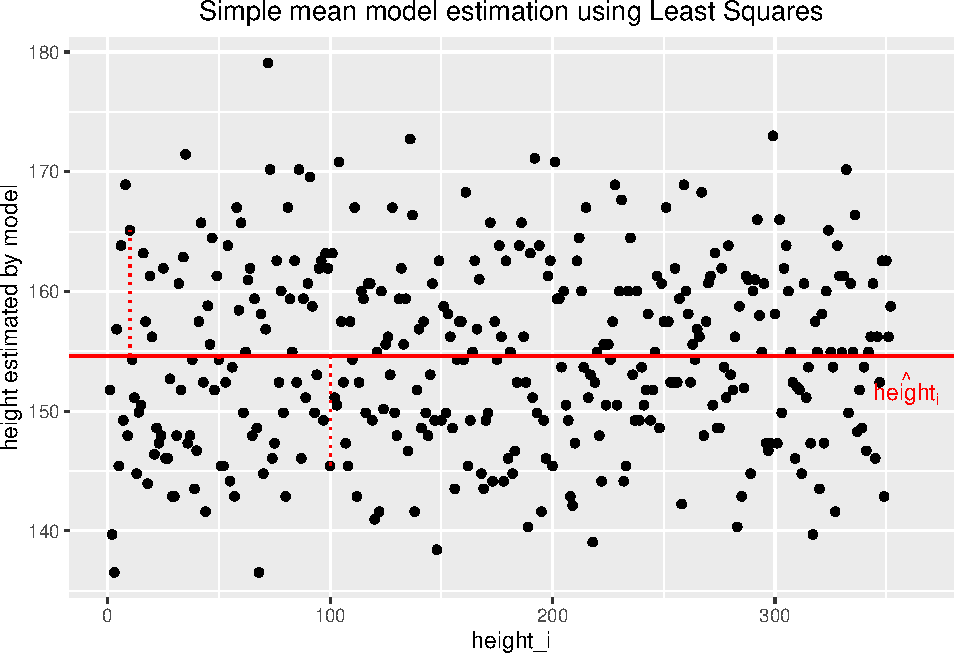
\includegraphics[keepaspectratio]{bookdown-demo_files/figure-latex/unnamed-chunk-16-1.pdf}}

Above, the heights are plotted against the index of the observation (the order does not matter).
The variability of heights around the regression line (constant in this case) seems to
stay constant, which is a good sign. We will call this
\href{https://en.wikipedia.org/wiki/Homoscedasticity_and_heteroscedasticity}{\textbf{homoscedasticity}} later.
The dashed vertical red lines show two residuals (one \(>0\), the other \(<0\)), the difference between the actual height
and the estimated height. The model-estimated heights (\(\widehat{heights_i}\))
are all identical and nothing but the mean of all heights.

Peter Westfall explains in his excellent book a \textbf{conditional distribution
approach} to regression, which is just what happens in the classical linear regression model.
I \textbf{highly recommend} reading the first chapters.

\textbf{What does this mean in this context?}
This means, that for every fixed value of the predictor (which we formally do not have),
the distribution of the response is normal with mean \(\hat{c}\) and standard deviation \(\sigma\).
Since, we do not have a predictor (apart from the intercept), we can say, that the distribution of the heights is normal with mean \(\hat{c}\)
and standard deviation \(\sigma\). This is what we assumed in the model. It can also be directly seen
in the formula:

\[ height_i = c + \varepsilon_i \]

If you add a normally distributed random variable (\(\varepsilon_i\)) to a constant (\(c\)),
the result is a normally distributed. No surprise here.

We can also create new data (heights) from this model and compare the distributions
of the actual data versus the model simulated data, since we have estimated the
parameter \(c\) and the standard deviation \(\sigma\).

\begin{Shaded}
\begin{Highlighting}[]
\NormalTok{c\_hat }\OtherTok{\textless{}{-}} \FunctionTok{mean}\NormalTok{(d2}\SpecialCharTok{$}\NormalTok{height)}
\NormalTok{sigma\_hat }\OtherTok{\textless{}{-}} \FunctionTok{sqrt}\NormalTok{(}\FunctionTok{sum}\NormalTok{(mod}\SpecialCharTok{$}\NormalTok{residuals}\SpecialCharTok{\^{}}\DecValTok{2}\NormalTok{) }\SpecialCharTok{/}\NormalTok{ (}\FunctionTok{nrow}\NormalTok{(d2) }\SpecialCharTok{{-}} \DecValTok{1}\NormalTok{))}

\CommentTok{\# simulate heights from model}
\NormalTok{heights\_sim }\OtherTok{\textless{}{-}} \FunctionTok{rnorm}\NormalTok{(}\FunctionTok{nrow}\NormalTok{(d2), c\_hat, sigma\_hat) }\CommentTok{\# as many as in orig.}

\CommentTok{\# Convert to data frames for plotting}
\NormalTok{df\_actual }\OtherTok{\textless{}{-}} \FunctionTok{data.frame}\NormalTok{(}\AttributeTok{height =}\NormalTok{ d2}\SpecialCharTok{$}\NormalTok{height, }\AttributeTok{type =} \StringTok{"Actual Heights"}\NormalTok{)}
\NormalTok{df\_simulated }\OtherTok{\textless{}{-}} \FunctionTok{data.frame}\NormalTok{(}\AttributeTok{height =}\NormalTok{ heights\_sim, }\AttributeTok{type =} \StringTok{"Simulated Heights"}\NormalTok{)}

\CommentTok{\# Combine the datasets}
\NormalTok{df\_combined }\OtherTok{\textless{}{-}} \FunctionTok{rbind}\NormalTok{(df\_actual, df\_simulated)}

\FunctionTok{ggplot}\NormalTok{(df\_combined, }\FunctionTok{aes}\NormalTok{(}\AttributeTok{x =}\NormalTok{ height, }\AttributeTok{fill =}\NormalTok{ type)) }\SpecialCharTok{+}
  \FunctionTok{geom\_density}\NormalTok{(}\AttributeTok{alpha =} \FloatTok{0.5}\NormalTok{) }\SpecialCharTok{+}
  \FunctionTok{labs}\NormalTok{(}\AttributeTok{title =} \StringTok{"Comparison of Actual and Model{-}Simulated Heights"}\NormalTok{,}
       \AttributeTok{x =} \StringTok{"Height"}\NormalTok{,}
       \AttributeTok{y =} \StringTok{"Density"}\NormalTok{) }\SpecialCharTok{+}
  \FunctionTok{scale\_fill\_manual}\NormalTok{(}\AttributeTok{values =} \FunctionTok{c}\NormalTok{(}\StringTok{"blue"}\NormalTok{, }\StringTok{"red"}\NormalTok{)) }\SpecialCharTok{+}
  \FunctionTok{theme\_minimal}\NormalTok{() }\SpecialCharTok{+}
  \FunctionTok{theme}\NormalTok{(}\AttributeTok{plot.title =} \FunctionTok{element\_text}\NormalTok{(}\AttributeTok{hjust =} \FloatTok{0.5}\NormalTok{))}
\end{Highlighting}
\end{Shaded}

\pandocbounded{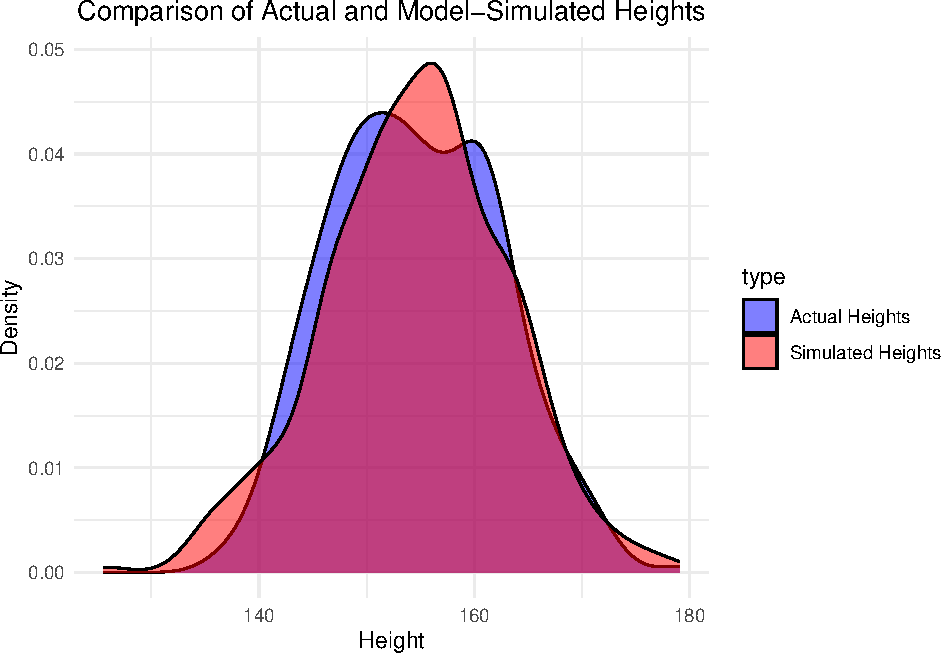
\includegraphics[keepaspectratio]{bookdown-demo_files/figure-latex/unnamed-chunk-17-1.pdf}}

One can repeat the simulation and see how the distributions changes to get
a feeling for the variability of the model/data.

\section{Exercises}\label{exercises}

{[}E{]} Easy, {[}M{]} Medium, {[}H{]} Hard

(Some) solutions to exercises can be found in the git-repo \href{https://github.com/jdegenfellner/Script_QM2_ZHAW/tree/main/Solutions_Exercises}{here}.

\subsection{{[}E{]} Exercise 1}\label{exercise1_Intro}

Use the \href{https://www.bfs.admin.ch/asset/de/30305714}{Swiss body heights} data to
determine

\begin{itemize}
\tightlist
\item
  the 95\% ``Vertrauensintervall'' for \(\mu\) and
\item
  calculate the standard deviation of the heights from \(21,873\) Swiss people.
\item
  Read the definition of the confidence interval in the footer of the table and
  explain why this is correct.
\end{itemize}

\subsection{{[}E{]} Exercise 2}\label{exercise2_Intro}

Why do we \textbf{not} need a hypothesis test to know that the population mean of body heights is not zero?
Give 2 reasons.

\subsection{{[}H{]} Exercise 3}\label{exercise3_Intro}

Verify analytically that the \texttt{Residual\ standard\ error} is identical with
the sample standard deviation of the heights in \hyperref[classical_simple_mean_model]{the simple mean model above}.

\subsection{{[}M{]} Exercise 4}\label{exercise4_Intro}

Repeat the Bayesian and Frequentist estimation of the simple model using a different data set about
\href{https://stat.ethz.ch/R-manual/R-devel/library/datasets/html/ChickWeight.html}{chicken weights},
which is included in R.

\begin{itemize}
\tightlist
\item
  Set useful priors for the mean and standard deviation of the model
  for the Baysian and the frequentist version considering
  your a priori knowledge about chicken weights.
\end{itemize}

\subsection{{[}M{]} Exercise 5}\label{exercise5_Intro}

\begin{itemize}
\tightlist
\item
  Try to understand/verify the code in the \hyperref[addendum]{addendum} below.
\item
  Change the parameters \(\mu = (\mu_X, \mu_Y)\) and \(\Sigma\) of the bivariate normal distribution
  and see how the 3D plot changes.
\item
  Plot the scatter plot of the \(X\) and \(Y\) values and compare it to the 3D plot.
  Does this make sense?
\item
  Why is the scatter plot elliptical?
\end{itemize}

\subsection{{[}M{]} Exercise 6}\label{exercise6_Intro}

Independence of two random variables \(X\) and \(Y\) implies that the
correlation between them is zero.
A correlation of zero does not necessarily imply independence.

\begin{itemize}
\tightlist
\item
  Verify this counterexample:
  For example, suppose the random variable \(X\) is symmetrically distributed about zero,
  and \(Y = X^2\). Then \(\mathit{Y}\) is completely determined by \(X\), so that
  \(\mathit{X}\) and \(\mathit{Y}\) are perfectly dependent, but their correlation is zero.
\end{itemize}

\subsection{{[}H{]} Exercise 7}\label{exercise7_Intro}

Go to the \hyperref[bivariate_normal]{section} aobut the bivariate normal distribution below.

\begin{itemize}
\tightlist
\item
  How do you get the correlation matrix from the covariance matrix (\(\Sigma\))?
  \[
  \Sigma =
  \begin{bmatrix}
  0.75 & 0.5 \\
  0.5 & 0.75
  \end{bmatrix}
  \]
  Hint: For the bivariate normal distribution, the correlation matrix is defined
  \href{https://en.wikipedia.org/wiki/Multivariate_normal_distribution\#Bivariate_case}{here}.
\end{itemize}

\section{Addendum}\label{addendum}

\subsection{The bivariate normal distribution}\label{bivariate_normal}

As a refresher, you can look into the old QM1 script and read the
chapter ``4.7 Gemeinsame Verteilungen''.
Maybe \href{https://www.youtube.com/watch?v=SP2GKq8xJ5I&ab_channel=StatisticsNinja}{this video}
also helps.

The \href{https://en.wikipedia.org/wiki/Multivariate_normal_distribution}{bivariate normal distribution}
is a generalization of the normal distribution to two dimensions.
Now, we look at the distribution of two random variables \(X\) and \(Y\) \textbf{at the same time}.

Instead of one Gaussian curve, we have a
\href{https://en.wikipedia.org/wiki/Multivariate_normal_distribution\#/media/File:Multivariate_Gaussian.png}{3D curve}.
This curve defines how plausible different combinations of \(X\) and \(Y\) are.

Single points (like (3,6)) still have probability zero, because now the \textbf{volume} over a single point
(\(x\), \(y\)) is zero. The probability of a certain area is now the \textbf{volume} under the
curve compared to the \textbf{area} under the density curve in the one-dimensional case.

\textbf{Example}: The following plot shows the density of a bivariate normal distribution of
two variables \(X\) and \(Y\)
with \(\mu_X = 0\), \(\mu_Y = 0\), \(\sigma_X = 1\), \(\sigma_Y = 1\) and \(\rho = \frac{2}{3}\).

Below is the correlation matrix of the bivariate normal distribution.

\begin{verbatim}
##           [,1]      [,2]
## [1,] 1.0000000 0.6666667
## [2,] 0.6666667 1.0000000
\end{verbatim}

\pandocbounded{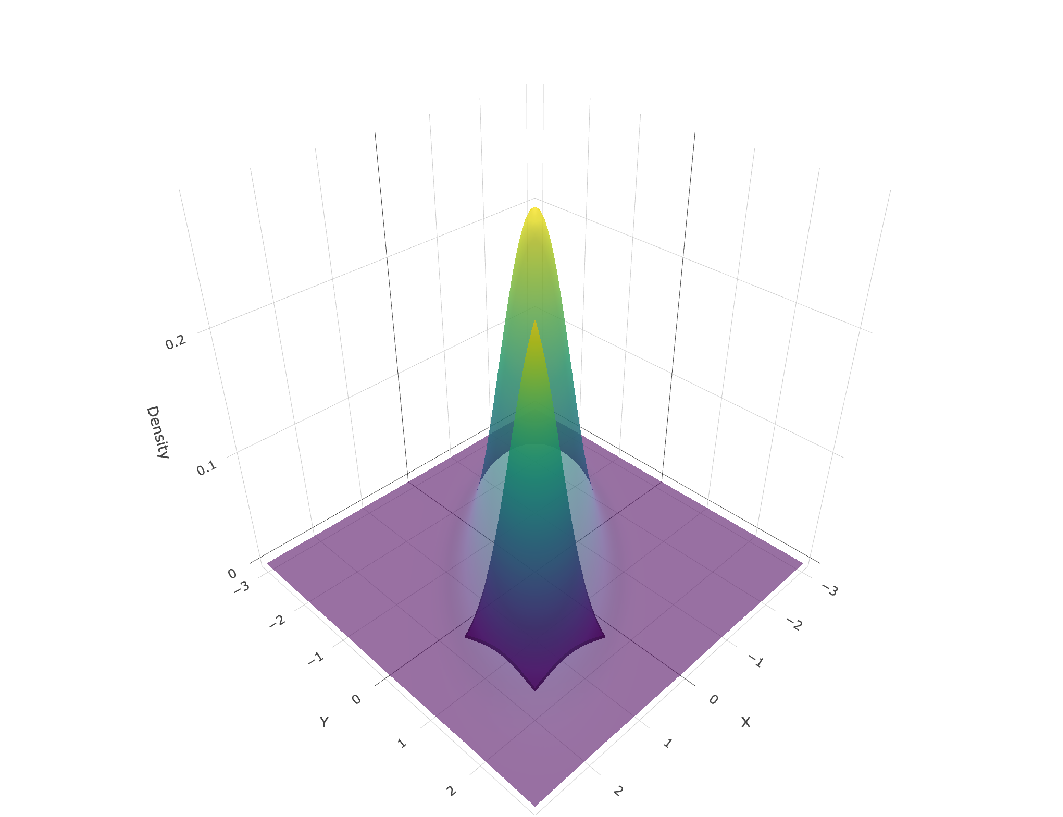
\includegraphics[keepaspectratio]{bookdown-demo_files/figure-latex/unnamed-chunk-18-1.pdf}}

If you move the plot around with your mouse, you see that there is a positive
correlation between \(X\) and \(Y\) (\(\rho = \frac{2}{3}\)). This means that if \(X\) is
above its mean, \(Y\) is also more likely to be above its mean.
The variances of \(X\) and \(Y\) are both \(1\). That means, that if you cut
through the plot in \(X=0\) or \(Y=0\), you see the same form of normal distribution.
If you look at if from above, we have hihglighted the section on the surface
over the area \(X \in [0.5, 2]\) and \(Y \in [0.5, 2]\). The volume over this area
under the density curve is the probability of this area: \(P(X \in [0.5, 2] \text{ and } Y \in [0.5, 2])\)

Calculate with R this probability with R:

\begin{Shaded}
\begin{Highlighting}[]
\CommentTok{\# Load the mvtnorm package}
\FunctionTok{library}\NormalTok{(mvtnorm)}

\CommentTok{\# Define the parameters of the bivariate normal distribution}
\NormalTok{mu }\OtherTok{\textless{}{-}} \FunctionTok{c}\NormalTok{(}\DecValTok{0}\NormalTok{, }\DecValTok{0}\NormalTok{)                       }\CommentTok{\# Mean}
\NormalTok{sigma }\OtherTok{\textless{}{-}} \FunctionTok{matrix}\NormalTok{(}\FunctionTok{c}\NormalTok{(}\FloatTok{0.75}\NormalTok{, }\FloatTok{0.5}\NormalTok{, }\FloatTok{0.5}\NormalTok{, }\FloatTok{0.75}\NormalTok{), }\AttributeTok{ncol =} \DecValTok{2}\NormalTok{) }\CommentTok{\# Covariance matrix}

\CommentTok{\# Define the bounds of the square}
\NormalTok{highlight\_x }\OtherTok{\textless{}{-}} \FunctionTok{c}\NormalTok{(}\FloatTok{0.5}\NormalTok{, }\DecValTok{2}\NormalTok{)}
\NormalTok{highlight\_y }\OtherTok{\textless{}{-}} \FunctionTok{c}\NormalTok{(}\FloatTok{0.5}\NormalTok{, }\DecValTok{2}\NormalTok{)}
\CommentTok{\# Calculate the probability using pmvnorm}
\FunctionTok{pmvnorm}\NormalTok{(}
  \AttributeTok{lower =} \FunctionTok{c}\NormalTok{(highlight\_x[}\DecValTok{1}\NormalTok{], highlight\_y[}\DecValTok{1}\NormalTok{]),}
  \AttributeTok{upper =} \FunctionTok{c}\NormalTok{(highlight\_x[}\DecValTok{2}\NormalTok{], highlight\_y[}\DecValTok{2}\NormalTok{]),}
  \AttributeTok{mean =}\NormalTok{ mu,}
  \AttributeTok{sigma =}\NormalTok{ sigma}
\NormalTok{)}
\end{Highlighting}
\end{Shaded}

\begin{verbatim}
## [1] 0.1526031
## attr(,"error")
## [1] 1e-15
## attr(,"msg")
## [1] "Normal Completion"
\end{verbatim}

Since we do not believe everything we are told, we rather check via simulation,
if \(0.1526\) is a plausible value for the probability:

\begin{Shaded}
\begin{Highlighting}[]
\CommentTok{\# Load necessary library}
\FunctionTok{library}\NormalTok{(MASS)}

\CommentTok{\# Define the parameters of the bivariate normal distribution}
\NormalTok{mu }\OtherTok{\textless{}{-}} \FunctionTok{c}\NormalTok{(}\DecValTok{0}\NormalTok{, }\DecValTok{0}\NormalTok{)                       }\CommentTok{\# Mean}
\NormalTok{sigma }\OtherTok{\textless{}{-}} \FunctionTok{matrix}\NormalTok{(}\FunctionTok{c}\NormalTok{(}\FloatTok{0.75}\NormalTok{, }\FloatTok{0.5}\NormalTok{, }\FloatTok{0.5}\NormalTok{, }\FloatTok{0.75}\NormalTok{), }\AttributeTok{ncol =} \DecValTok{2}\NormalTok{) }\CommentTok{\# Covariance matrix}
\FunctionTok{cov2cor}\NormalTok{(sigma)  }\CommentTok{\# Convert covariance matrix to correlation matrix}
\end{Highlighting}
\end{Shaded}

\begin{verbatim}
##           [,1]      [,2]
## [1,] 1.0000000 0.6666667
## [2,] 0.6666667 1.0000000
\end{verbatim}

\begin{Shaded}
\begin{Highlighting}[]
\CommentTok{\# Define the bounds of the square}
\NormalTok{highlight\_x }\OtherTok{\textless{}{-}} \FunctionTok{c}\NormalTok{(}\FloatTok{0.5}\NormalTok{, }\DecValTok{2}\NormalTok{)}
\NormalTok{highlight\_y }\OtherTok{\textless{}{-}} \FunctionTok{c}\NormalTok{(}\FloatTok{0.5}\NormalTok{, }\DecValTok{2}\NormalTok{)}

\CommentTok{\# Number of simulations}
\NormalTok{n\_sim }\OtherTok{\textless{}{-}} \DecValTok{10}\SpecialCharTok{\^{}}\DecValTok{4}

\FunctionTok{set.seed}\NormalTok{(}\DecValTok{343434}\NormalTok{)}
\CommentTok{\# Simulate bivariate normal samples}
\NormalTok{samples }\OtherTok{\textless{}{-}} \FunctionTok{mvrnorm}\NormalTok{(}\AttributeTok{n =}\NormalTok{ n\_sim, }\AttributeTok{mu =}\NormalTok{ mu, }\AttributeTok{Sigma =}\NormalTok{ sigma)}

\CommentTok{\# Count how many samples fall within the square}
\NormalTok{inside\_square }\OtherTok{\textless{}{-}} \FunctionTok{sum}\NormalTok{(}
\NormalTok{  samples[, }\DecValTok{1}\NormalTok{] }\SpecialCharTok{\textgreater{}=}\NormalTok{ highlight\_x[}\DecValTok{1}\NormalTok{] }\SpecialCharTok{\&}\NormalTok{ samples[, }\DecValTok{1}\NormalTok{] }\SpecialCharTok{\textless{}=}\NormalTok{ highlight\_x[}\DecValTok{2}\NormalTok{] }\SpecialCharTok{\&}
\NormalTok{  samples[, }\DecValTok{2}\NormalTok{] }\SpecialCharTok{\textgreater{}=}\NormalTok{ highlight\_y[}\DecValTok{1}\NormalTok{] }\SpecialCharTok{\&}\NormalTok{ samples[, }\DecValTok{2}\NormalTok{] }\SpecialCharTok{\textless{}=}\NormalTok{ highlight\_y[}\DecValTok{2}\NormalTok{]}
\NormalTok{)}

\CommentTok{\# Estimate the probability}
\NormalTok{inside\_square }\SpecialCharTok{/}\NormalTok{ n\_sim}
\end{Highlighting}
\end{Shaded}

\begin{verbatim}
## [1] 0.1557
\end{verbatim}

Looks good.

\chapter{Simple Linear Regression}\label{simple-linear-regression}

\section{Simple Linear Regression in the Bayesian Framework}\label{simple_lin_reg_bayes}

You can watch \href{https://www.youtube.com/watch?v=14mkCpJ7tKs&ab_channel=VeryNormal}{this video} as primer.

We will now add one covariate/explanatory variable to the model.
Refer to \href{https://civil.colorado.edu/~balajir/CVEN6833/bayes-resources/RM-StatRethink-Bayes.pdf}{Statistical Rethinking}
``4.4 Linear prediction'' or ``4.4 Adding a predictor'' as it's called in the online version of the book.

So far, our ``regression'' did not do much to be honest. The mean of a list of values
was already calculated in the \href{https://jdegenfellner.github.io/Script_QM1_ZHAW/descriptive_stats.html}{descriptive statistics section}
before and we have mentioned how great this statistic is as measure of location and where its weaknesses are.

Now, we want to model \textbf{how} body height and weight are \textbf{related}.
Formally, one wants to \emph{predict} body heights from body weights.

Here and in the Frequentist framework, we will see that it is \textbf{not the same}
problem (and therefore results in a different statistical model)
\textbf{to predict body weights from body heights or vice versa}.

We remember the following:

\begin{itemize}
\tightlist
\item
  Regress \(Y\) on \(X\), which is equivalent to predict \(Y\) from \(X\).
  We know X and want to predict Y.
\item
  Regress \(X\) on \(Y\), which is equivalent to predict \(X\) from \(Y\).
  We know Y and want to predict X.
\end{itemize}

The word ``predictor'' is important here. It is a technical term
and describes a variable that we know (in our case weight) and with
which we want to ``guess as good as possible'' the value of the
dependent variable (in our case height). ``As good as possible''
means that we put a penalty on an error. The farer our prediction
is away from the true value (\(y_i\)), the higher the penalty.
And not only that, but if you are twice as far away from the true value,
you should be penalized four times as much. This is the idea behind
the squared error \href{https://en.wikipedia.org/wiki/Loss_function}{loss function}
and the core of the least squares method.
What if we would punish differently, you ask?
There are many loss functions one could use
(for instance the \href{https://en.wikipedia.org/wiki/Huber_loss}{Huber loss}),
maybe we will see some later. For now, we punish quadratically.

We \textbf{always} visualize the data first to improve our understanding.
First comes descriptive statistics, then one can think about modeling.

\begin{Shaded}
\begin{Highlighting}[]
\FunctionTok{plot}\NormalTok{(d2}\SpecialCharTok{$}\NormalTok{height }\SpecialCharTok{\textasciitilde{}}\NormalTok{ d2}\SpecialCharTok{$}\NormalTok{weight)}
\end{Highlighting}
\end{Shaded}

\pandocbounded{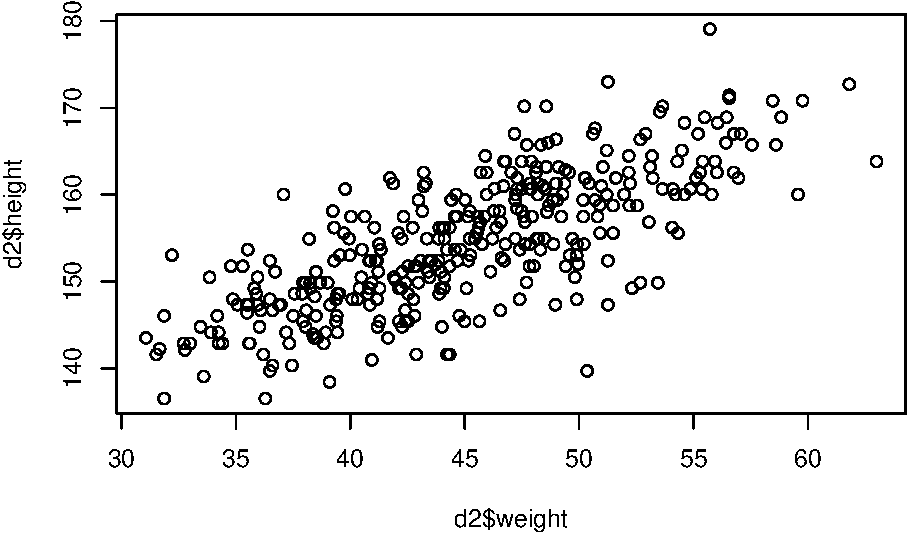
\includegraphics[keepaspectratio]{bookdown-demo_files/figure-latex/unnamed-chunk-21-1.pdf}}

It's not often that you see such a clean plot.
The scatterplot indicates a linear relationship between the two variables.
The higher the weight, the higher the height; with some deviations of course and
we decide that normally distributed errors are a good idea.
This relationsip is neither causal, nor deterministic.

\begin{itemize}
\tightlist
\item
  It is not causal since an increase in weight does not
  necessarily lead to an increase in height, especially in grown-ups.
\item
  It is not deterministic since there are deviations from the line.
  It if was deterministic, we would not need statistical modeling.
\end{itemize}

For simpler notation, we will call \texttt{d2\$weight} \(x\). \(\bar{x}\)
is the mean of \(x\).

\subsection{Model definition}\label{model-definition}

Let's write down our \textbf{model} (again with the Swiss population prior mean):

\begin{eqnarray*}
h_i &\sim& \text{Normal}(\mu_i, \sigma)\\
\mu_i &\sim& \alpha + \beta (x_i - \bar{x})\\
\alpha &\sim& \text{Normal}(171.1, 20)\\
\beta &\sim& \text{Normal}(0, 10)\\
\sigma &\sim& \text{Uniform}(0, 50)
\end{eqnarray*}

Visualization of the \textbf{model structure}:

\begin{verbatim}
## file:////private/var/folders/pm/jd6n6gj10371_bml1gh8sc5w0000gn/T/RtmpOZ9C46/file5f90642b334d/widget5f905035379b.html screenshot completed
\end{verbatim}

\pandocbounded{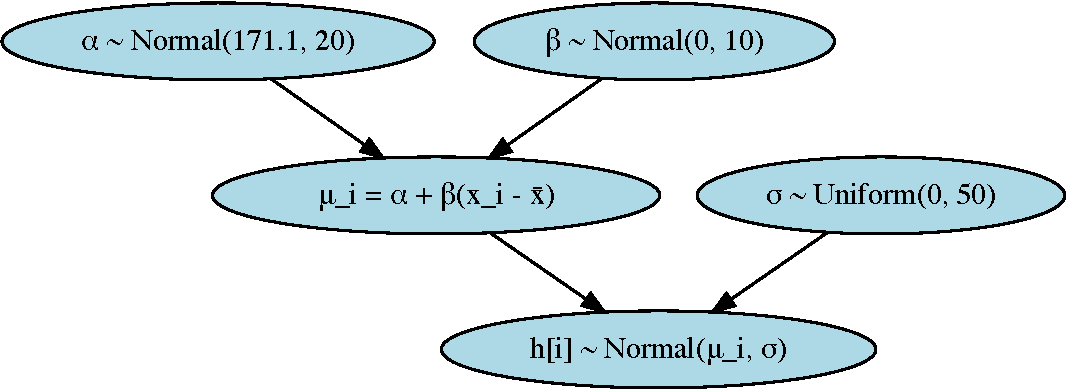
\includegraphics[keepaspectratio]{bookdown-demo_files/figure-latex/unnamed-chunk-22-1.pdf}}

There are now additional lines for the priors of \(\alpha\) and \(\beta\)
(compared to the simple mean model before).
The model structure also shows the way to simulate from the prior.
One starts at the top and ends up with the heights.

\begin{itemize}
\tightlist
\item
  \(h_i\) is the height of the \(i\)-th person and we assume it is normally distributed.
\item
  \(\mu_i\) is the mean of the height of the \(i\)-th person and we
  assume it is linearly dependent on the difference \(x_i-\bar{x}\).
  Compared to the intercept model, a different mean is assumed for each person
  depending on his/her weight.
\item
  \(\alpha\) is the intercept and we use the same prior as before.
\item
  \(\beta\) is the slope of the line and we use the normal distribution as prior for it,
  hence it can be positive or negative and how plausible each value is, is
  determined by that specific normal distribution. Note, that we could
  easily adapt the distribution to any distribution we like.
\item
  The prior for \(\sigma\) is unchanged.
\item
  \(x_i - \bar{x}\) is the deviation of the weight from the mean weight, thereby \textbf{we
  center} the weight variable. This is a common practice in regression analysis.
  A value \(x_i - \bar{x} > 0\) implies that the person is heavier than the average.
\end{itemize}

The linear model is quite popular in applied statistics and one
reason is probably the rather straightforward interpretation of the coefficients:
A one unit increase in weight is on average (in the mean) associated with
a \(\beta\) unit increase/decrease (depending if \(\beta\) is \(>0\) or \(<0\)) in height.

\subsection{Priors}\label{priors}

We want to plot our prior predictions to get a feeling \textbf{what
the model would predict without seeing the data}.
This is a kind of ``sanity check'' to see if the priors and
the model definition are reasonable.
Again, we just draw from the assumed distributions for \(\alpha\) and \(\beta\)
100 times and draw the corresponding lines. Just as the model
definition says.

\begin{Shaded}
\begin{Highlighting}[]
\FunctionTok{set.seed}\NormalTok{(}\DecValTok{2971}\NormalTok{)}
\NormalTok{N }\OtherTok{\textless{}{-}} \DecValTok{100}  \CommentTok{\# 100 lines}
\NormalTok{a }\OtherTok{\textless{}{-}} \FunctionTok{rnorm}\NormalTok{(N, }\FloatTok{171.1}\NormalTok{, }\DecValTok{20}\NormalTok{)}
\NormalTok{b }\OtherTok{\textless{}{-}} \FunctionTok{rnorm}\NormalTok{(N, }\DecValTok{0}\NormalTok{, }\DecValTok{10}\NormalTok{)}

\NormalTok{xbar }\OtherTok{\textless{}{-}} \FunctionTok{mean}\NormalTok{(d2}\SpecialCharTok{$}\NormalTok{weight)}

\CommentTok{\# start with empty plot}
\FunctionTok{plot}\NormalTok{(}\ConstantTok{NULL}\NormalTok{, }\AttributeTok{xlim =} \FunctionTok{range}\NormalTok{(d2}\SpecialCharTok{$}\NormalTok{weight), }\AttributeTok{ylim =} \FunctionTok{c}\NormalTok{(}\SpecialCharTok{{-}}\DecValTok{100}\NormalTok{, }\DecValTok{400}\NormalTok{),}
     \AttributeTok{xlab =} \StringTok{"weight"}\NormalTok{, }\AttributeTok{ylab =} \StringTok{"height"}\NormalTok{)}
\FunctionTok{abline}\NormalTok{(}\AttributeTok{h =} \DecValTok{0}\NormalTok{, }\AttributeTok{lty =} \DecValTok{2}\NormalTok{)  }\CommentTok{\# horizontal line at 0}
\FunctionTok{abline}\NormalTok{(}\AttributeTok{h =} \DecValTok{272}\NormalTok{, }\AttributeTok{lty =} \DecValTok{1}\NormalTok{, }\AttributeTok{lwd =} \FloatTok{0.5}\NormalTok{)  }\CommentTok{\# horizontal line at 272}
\FunctionTok{mtext}\NormalTok{(}\StringTok{"b \textasciitilde{} dnorm(0, 10)"}\NormalTok{)}

\CommentTok{\# Overlay the 100 lines}
\ControlFlowTok{for}\NormalTok{ (i }\ControlFlowTok{in} \DecValTok{1}\SpecialCharTok{:}\NormalTok{N) \{}
  \FunctionTok{curve}\NormalTok{(a[i] }\SpecialCharTok{+}\NormalTok{ b[i] }\SpecialCharTok{*}\NormalTok{ (x }\SpecialCharTok{{-}}\NormalTok{ xbar),}
        \AttributeTok{from =} \FunctionTok{min}\NormalTok{(d2}\SpecialCharTok{$}\NormalTok{weight), }\AttributeTok{to =} \FunctionTok{max}\NormalTok{(d2}\SpecialCharTok{$}\NormalTok{weight),}
        \AttributeTok{add =} \ConstantTok{TRUE}\NormalTok{, }\AttributeTok{col =} \FunctionTok{col.alpha}\NormalTok{(}\StringTok{"black"}\NormalTok{, }\FloatTok{0.2}\NormalTok{))}
\NormalTok{\}}
\end{Highlighting}
\end{Shaded}

\pandocbounded{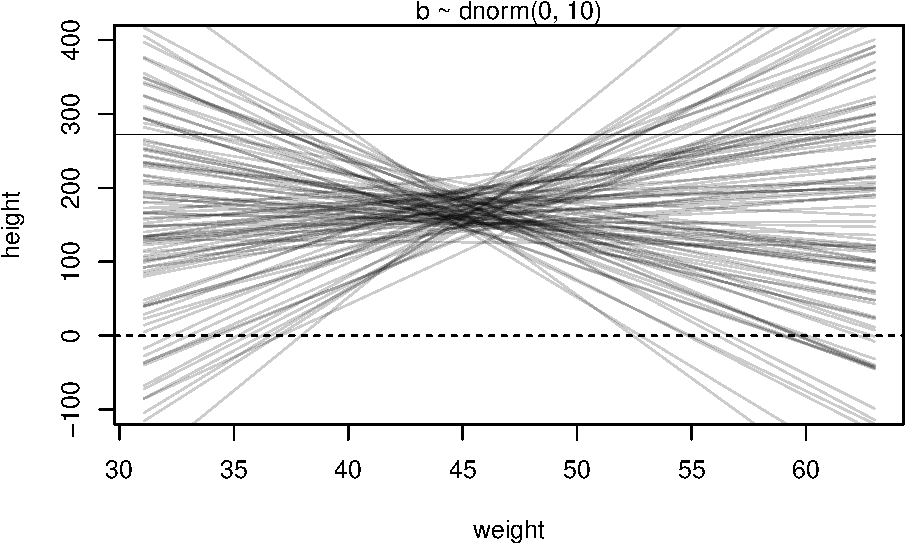
\includegraphics[keepaspectratio]{bookdown-demo_files/figure-latex/unnamed-chunk-23-1.pdf}}

This linear relationship defined with the chosen priors seems rather
non-restrictive. According to our priors,
one could see very steeply rising or falling relationships between weight and expected heights.
We could at least make the priors for the slope (\(\beta\)) non-negative.
One possibility to do this
is to use a \href{https://en.wikipedia.org/wiki/Log-normal_distribution}{log-normal distribution}
for the prior of \(\beta\) which can only take non-negative values.

\[ \beta \sim \text{Log-Normal}(0, 1) \]

Lets plot the priors again.

\begin{Shaded}
\begin{Highlighting}[]
\FunctionTok{set.seed}\NormalTok{(}\DecValTok{2971}\NormalTok{)}
\NormalTok{N }\OtherTok{\textless{}{-}} \DecValTok{100}  \CommentTok{\# 100 lines}
\NormalTok{a }\OtherTok{\textless{}{-}} \FunctionTok{rnorm}\NormalTok{(N, }\FloatTok{171.1}\NormalTok{, }\DecValTok{20}\NormalTok{)}
\NormalTok{b }\OtherTok{\textless{}{-}} \FunctionTok{rlnorm}\NormalTok{(N, }\DecValTok{0}\NormalTok{, }\DecValTok{1}\NormalTok{)}

\NormalTok{xbar }\OtherTok{\textless{}{-}} \FunctionTok{mean}\NormalTok{(d2}\SpecialCharTok{$}\NormalTok{weight)}

\FunctionTok{plot}\NormalTok{(}\ConstantTok{NULL}\NormalTok{, }\AttributeTok{xlim =} \FunctionTok{range}\NormalTok{(d2}\SpecialCharTok{$}\NormalTok{weight), }\AttributeTok{ylim =} \FunctionTok{c}\NormalTok{(}\SpecialCharTok{{-}}\DecValTok{100}\NormalTok{, }\DecValTok{400}\NormalTok{),}
     \AttributeTok{xlab =} \StringTok{"weight"}\NormalTok{, }\AttributeTok{ylab =} \StringTok{"height"}\NormalTok{)}
\FunctionTok{abline}\NormalTok{(}\AttributeTok{h =} \DecValTok{0}\NormalTok{, }\AttributeTok{lty =} \DecValTok{2}\NormalTok{)  }\CommentTok{\# horizontal line at 0}
\FunctionTok{abline}\NormalTok{(}\AttributeTok{h =} \DecValTok{272}\NormalTok{, }\AttributeTok{lty =} \DecValTok{1}\NormalTok{, }\AttributeTok{lwd =} \FloatTok{0.5}\NormalTok{)  }\CommentTok{\# horizontal line at 272}
\FunctionTok{mtext}\NormalTok{(}\StringTok{"b \textasciitilde{} dlnorm(0, 1)"}\NormalTok{)}

\CommentTok{\# Overlay the 100 lines}
\ControlFlowTok{for}\NormalTok{ (i }\ControlFlowTok{in} \DecValTok{1}\SpecialCharTok{:}\NormalTok{N) \{}
  \FunctionTok{curve}\NormalTok{(a[i] }\SpecialCharTok{+}\NormalTok{ b[i] }\SpecialCharTok{*}\NormalTok{ (x }\SpecialCharTok{{-}}\NormalTok{ xbar),}
        \AttributeTok{from =} \FunctionTok{min}\NormalTok{(d2}\SpecialCharTok{$}\NormalTok{weight), }\AttributeTok{to =} \FunctionTok{max}\NormalTok{(d2}\SpecialCharTok{$}\NormalTok{weight),}
        \AttributeTok{add =} \ConstantTok{TRUE}\NormalTok{, }\AttributeTok{col =} \FunctionTok{col.alpha}\NormalTok{(}\StringTok{"black"}\NormalTok{, }\FloatTok{0.2}\NormalTok{))}
\NormalTok{\}}
\end{Highlighting}
\end{Shaded}

\pandocbounded{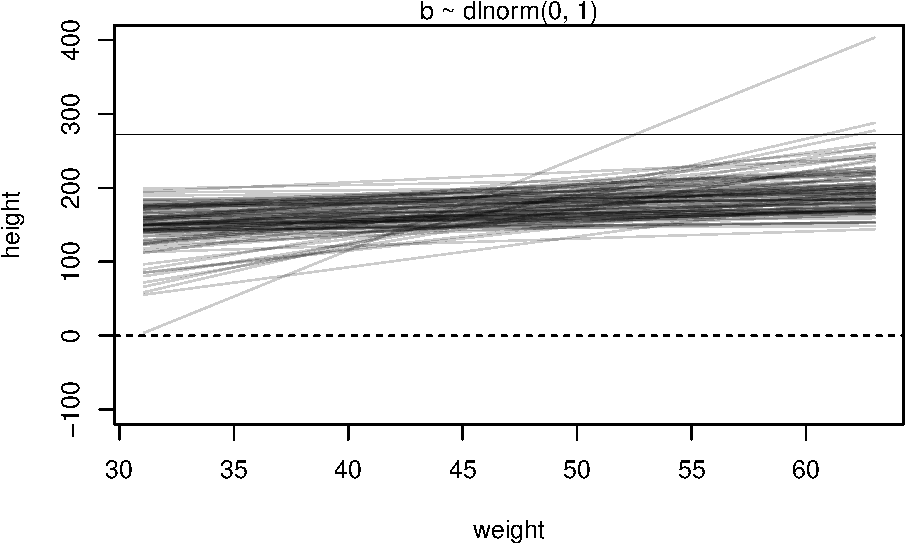
\includegraphics[keepaspectratio]{bookdown-demo_files/figure-latex/unnamed-chunk-24-1.pdf}}

This seems definitely more realistic. There is some sort of positive linear relationship
between weight and expected height.

\subsection{Fit model}\label{fit-model}

Now, let's \textbf{estimate the posterior/fit the model} as before:

\begin{Shaded}
\begin{Highlighting}[]
\CommentTok{\# load data again, since it\textquotesingle{}s a long way back}
\FunctionTok{library}\NormalTok{(rethinking)}
\FunctionTok{data}\NormalTok{(Howell1)}
\NormalTok{d }\OtherTok{\textless{}{-}}\NormalTok{ Howell1}
\NormalTok{d2 }\OtherTok{\textless{}{-}}\NormalTok{ d[d}\SpecialCharTok{$}\NormalTok{age }\SpecialCharTok{\textgreater{}=} \DecValTok{18}\NormalTok{, ]}
\NormalTok{xbar }\OtherTok{\textless{}{-}} \FunctionTok{mean}\NormalTok{(d2}\SpecialCharTok{$}\NormalTok{weight)}
\CommentTok{\# fit model}
\NormalTok{mod }\OtherTok{\textless{}{-}} \FunctionTok{quap}\NormalTok{(}
    \FunctionTok{alist}\NormalTok{(}
\NormalTok{        height }\SpecialCharTok{\textasciitilde{}} \FunctionTok{dnorm}\NormalTok{(mu, sigma),}
\NormalTok{        mu }\OtherTok{\textless{}{-}}\NormalTok{ a }\SpecialCharTok{+}\NormalTok{ b }\SpecialCharTok{*}\NormalTok{ (weight }\SpecialCharTok{{-}}\NormalTok{ xbar),}
\NormalTok{        a }\SpecialCharTok{\textasciitilde{}} \FunctionTok{dnorm}\NormalTok{(}\FloatTok{171.1}\NormalTok{, }\DecValTok{100}\NormalTok{),}
\NormalTok{        b }\SpecialCharTok{\textasciitilde{}} \FunctionTok{dnorm}\NormalTok{(}\DecValTok{0}\NormalTok{, }\DecValTok{10}\NormalTok{),}
\NormalTok{        sigma }\SpecialCharTok{\textasciitilde{}} \FunctionTok{dunif}\NormalTok{(}\DecValTok{0}\NormalTok{, }\DecValTok{50}\NormalTok{)}
\NormalTok{    ) ,}
\AttributeTok{data =}\NormalTok{ d2)}
\end{Highlighting}
\end{Shaded}

Note that the model definition was now directly included in the \texttt{quap} function.
Let's look at the \textbf{marginal distributions} of the parameters:

\begin{Shaded}
\begin{Highlighting}[]
\FunctionTok{precis}\NormalTok{(mod)}
\end{Highlighting}
\end{Shaded}

\begin{verbatim}
##              mean         sd        5.5%       94.5%
## a     154.5972120 0.27033045 154.1651717 155.0292523
## b       0.9050131 0.04192754   0.8380048   0.9720214
## sigma   5.0718673 0.19115323   4.7663675   5.3773671
\end{verbatim}

\begin{Shaded}
\begin{Highlighting}[]
\FunctionTok{plot}\NormalTok{(mod)}
\end{Highlighting}
\end{Shaded}

\pandocbounded{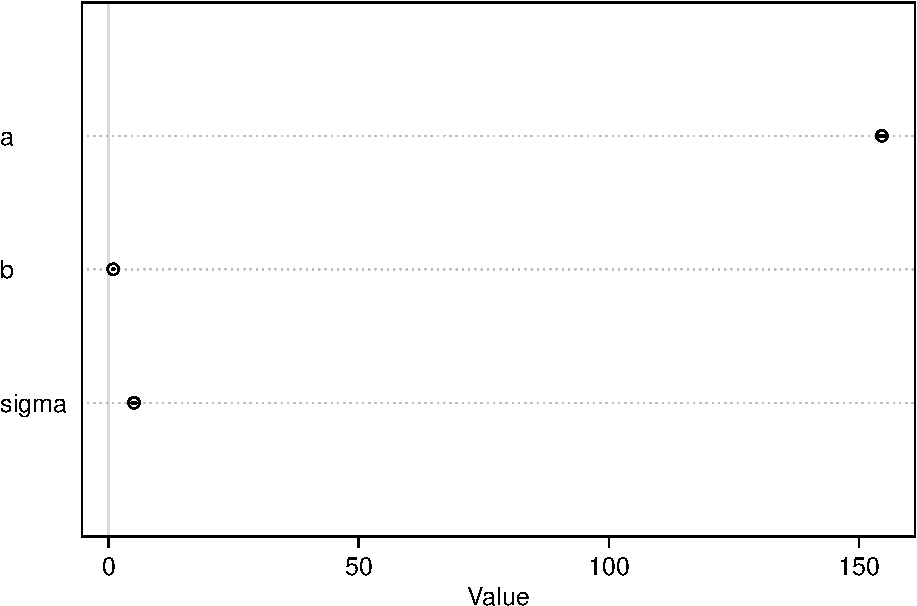
\includegraphics[keepaspectratio]{bookdown-demo_files/figure-latex/unnamed-chunk-26-1.pdf}}

Note, that the credible intervals in the plot of the coefficients are
hardly noticable. The reason is that the intercept \(a\) is rather large,
whereas \(b\) and sigma are comparativly small. The plot is scaled to the
largest parameter.

We can improve this by centering the height variable as well. Or,
we could standardize both weight and height. This would change the interpretation
of the \(\beta\) parameter. It would then be the expected change in standard deviations
when changing weight by one standard deviation.
See \hyperref[exercise12_simpl_lin_reg]{exercise 12}.

The analysis yields estimates for all our parameters of the model: \(\alpha\),
\(\beta\) and \(\sigma\). The estimates are the mean of the posterior distribution.

See \hyperref[exercise2_simpl_lin_reg]{exercise 2}.

\textbf{Interpretation of \(\beta\)}:
The mean of the posterior distribution of \(\beta\) is 0.9. A person with a weight
of 1 kg more weight can be expected to be 0.9 cm taller. A 89\% credible interval
for this estimate is \([0.83, 0.97]\). We can be quite sure that the slope is
positive (of course we designed it that way too via the prior).

It might also be interesting to inspect the \textbf{variance-covariance matrix},
respectively the correlation between the parameters as we did before
in the intercept model. Remember, these are the correlations of
parameters in the multivariate (because three paremeters simulatenously)
posterior distribution.

\begin{Shaded}
\begin{Highlighting}[]
\FunctionTok{diag}\NormalTok{(}\FunctionTok{vcov}\NormalTok{(mod))}
\end{Highlighting}
\end{Shaded}

\begin{verbatim}
##           a           b       sigma 
## 0.073078550 0.001757918 0.036539558
\end{verbatim}

\begin{Shaded}
\begin{Highlighting}[]
\FunctionTok{round}\NormalTok{(}\FunctionTok{cov2cor}\NormalTok{(}\FunctionTok{vcov}\NormalTok{(mod)),}\DecValTok{2}\NormalTok{)}
\end{Highlighting}
\end{Shaded}

\begin{verbatim}
##       a b sigma
## a     1 0     0
## b     0 1     0
## sigma 0 0     1
\end{verbatim}

\begin{itemize}
\tightlist
\item
  \texttt{diag(vcov(mod))} gives the variances of the parameters and
\item
  \texttt{cov2cor(vcov(mod))}the correlations. As we can see the correlations are (near) zero. Compare to the graphical
  display of the model structure. There is no connection.
\end{itemize}

\subsection{Result}\label{result}

\textbf{Graphical end result} of fitting the model:
We plot the marginal posterior distributions of \(\alpha\) and \(\beta\),
and also the raw data with the found regression line.

\begin{Shaded}
\begin{Highlighting}[]
\NormalTok{post }\OtherTok{\textless{}{-}} \FunctionTok{extract.samples}\NormalTok{(mod)}
\FunctionTok{dens}\NormalTok{(post}\SpecialCharTok{$}\NormalTok{a, }\AttributeTok{col =}\NormalTok{ rangi2)}
\end{Highlighting}
\end{Shaded}

\pandocbounded{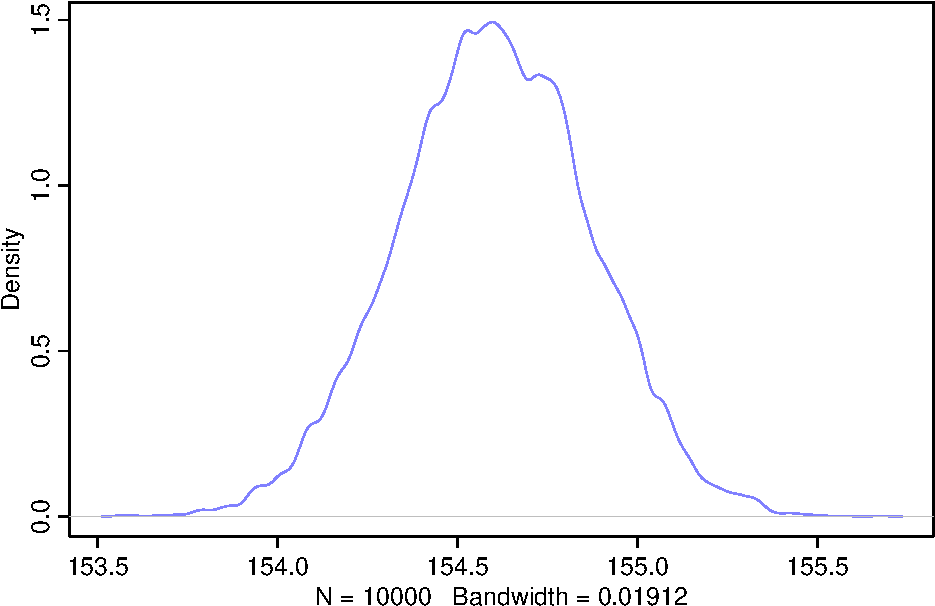
\includegraphics[keepaspectratio]{bookdown-demo_files/figure-latex/unnamed-chunk-28-1.pdf}}

\begin{Shaded}
\begin{Highlighting}[]
\FunctionTok{dens}\NormalTok{(post}\SpecialCharTok{$}\NormalTok{b, }\AttributeTok{col =}\NormalTok{ rangi2)}
\end{Highlighting}
\end{Shaded}

\pandocbounded{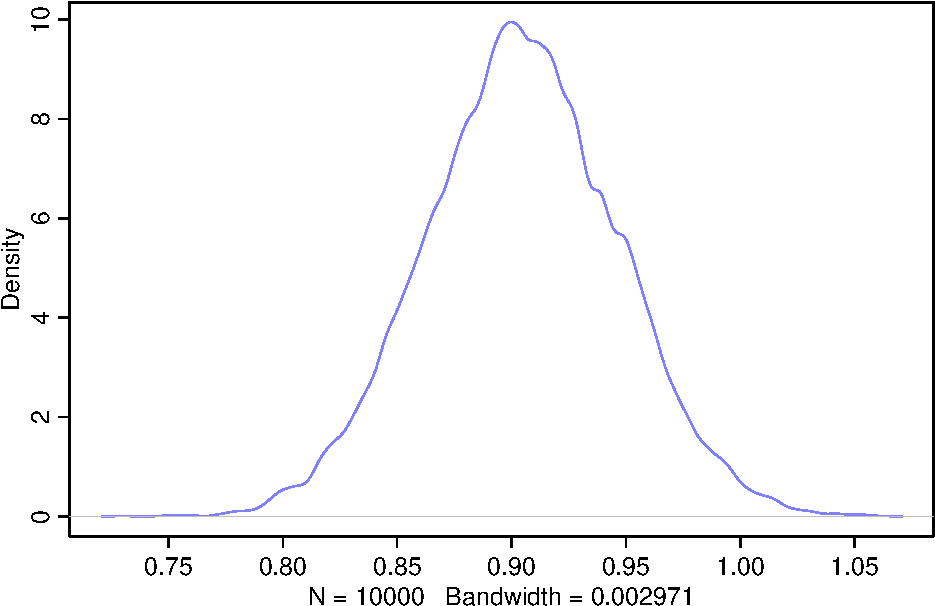
\includegraphics[keepaspectratio]{bookdown-demo_files/figure-latex/unnamed-chunk-28-2.pdf}}

\begin{Shaded}
\begin{Highlighting}[]
\CommentTok{\# both posteror plots seem symmetric}
\CommentTok{\# we use the mean as point estimate}
\CommentTok{\# for a and b.}
\NormalTok{a\_quap }\OtherTok{\textless{}{-}} \FunctionTok{mean}\NormalTok{(post}\SpecialCharTok{$}\NormalTok{a)}
\NormalTok{b\_quap }\OtherTok{\textless{}{-}} \FunctionTok{mean}\NormalTok{(post}\SpecialCharTok{$}\NormalTok{b)}

\FunctionTok{plot}\NormalTok{(d2}\SpecialCharTok{$}\NormalTok{height }\SpecialCharTok{\textasciitilde{}}\NormalTok{ d2}\SpecialCharTok{$}\NormalTok{weight, }\AttributeTok{col =}\NormalTok{ rangi2)}
\FunctionTok{curve}\NormalTok{(a\_quap }\SpecialCharTok{+}\NormalTok{ b\_quap }\SpecialCharTok{*}\NormalTok{ (x }\SpecialCharTok{{-}}\NormalTok{ xbar), }\AttributeTok{add =} \ConstantTok{TRUE}\NormalTok{)}
\end{Highlighting}
\end{Shaded}

\pandocbounded{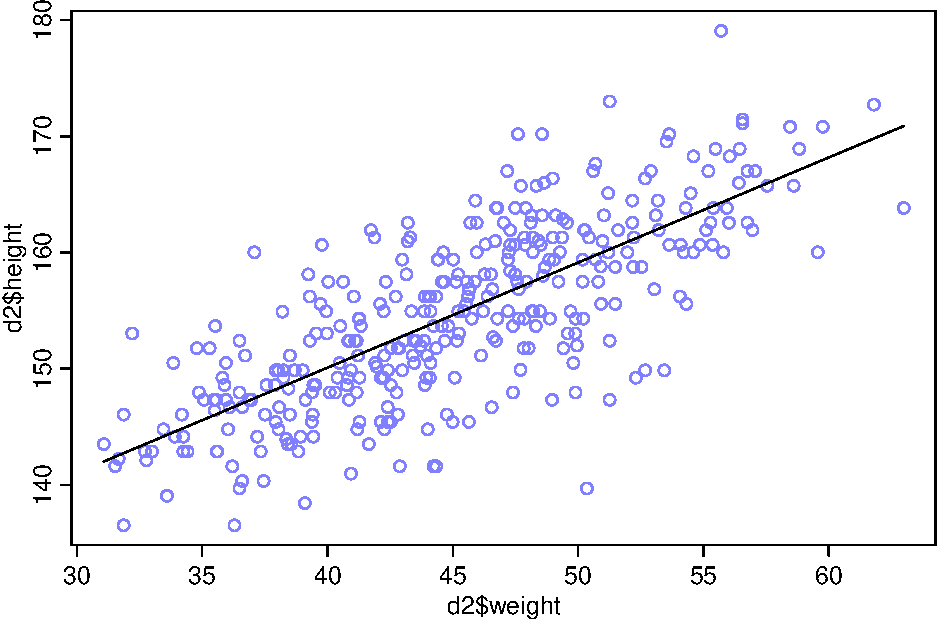
\includegraphics[keepaspectratio]{bookdown-demo_files/figure-latex/unnamed-chunk-28-3.pdf}}

\subsection{Credible bands}\label{credible-bands}

We could draw again and again from the posterior distribution
and calculate the means like above. Plotting the regression lines
with the respective parameters \(\alpha\), \(\beta\) would indicate
the variability of the estimates.
Note that we do not draw from the data (as one does in bootstrap resampling),
but from the posterior distribution.
The \texttt{link} function does this for us. It takes the posterior distribution we
have just fit, samples \(\alpha\) and \(\beta\) from it, calculates the mean and then
samples from this normal distribution for the mean at a given weight.
Refer to pages 98-106 in the current version of the book Statistical Rethinking
for all details.

\begin{Shaded}
\begin{Highlighting}[]
\CommentTok{\# Define a sequence of weights for predictions}
\NormalTok{weight.seq }\OtherTok{\textless{}{-}} \FunctionTok{seq}\NormalTok{(}\AttributeTok{from =} \DecValTok{25}\NormalTok{, }\AttributeTok{to =} \DecValTok{70}\NormalTok{, }\AttributeTok{by =} \DecValTok{1}\NormalTok{)}

\CommentTok{\# Use the model to compute mu for each weight}
\NormalTok{mu }\OtherTok{\textless{}{-}} \FunctionTok{link}\NormalTok{(mod, }\AttributeTok{data =} \FunctionTok{data.frame}\NormalTok{(}\AttributeTok{weight =}\NormalTok{ weight.seq))}
\FunctionTok{str}\NormalTok{(mu)}
\end{Highlighting}
\end{Shaded}

\begin{verbatim}
##  num [1:1000, 1:46] 138 136 137 136 137 ...
\end{verbatim}

\begin{Shaded}
\begin{Highlighting}[]
\CommentTok{\# Visualize the distribution of mu values}
\FunctionTok{plot}\NormalTok{(height }\SpecialCharTok{\textasciitilde{}}\NormalTok{ weight, d2, }\AttributeTok{type =} \StringTok{"n"}\NormalTok{)  }\CommentTok{\# Hide raw data with type = "n"}

\CommentTok{\# Loop over samples and plot each mu value}
\ControlFlowTok{for}\NormalTok{ (i }\ControlFlowTok{in} \DecValTok{1}\SpecialCharTok{:}\DecValTok{100}\NormalTok{) \{}
  \FunctionTok{points}\NormalTok{(weight.seq, mu[i, ], }\AttributeTok{pch =} \DecValTok{16}\NormalTok{, }\AttributeTok{col =} \FunctionTok{col.alpha}\NormalTok{(rangi2, }\FloatTok{0.1}\NormalTok{))}
\NormalTok{\}}
\end{Highlighting}
\end{Shaded}

\pandocbounded{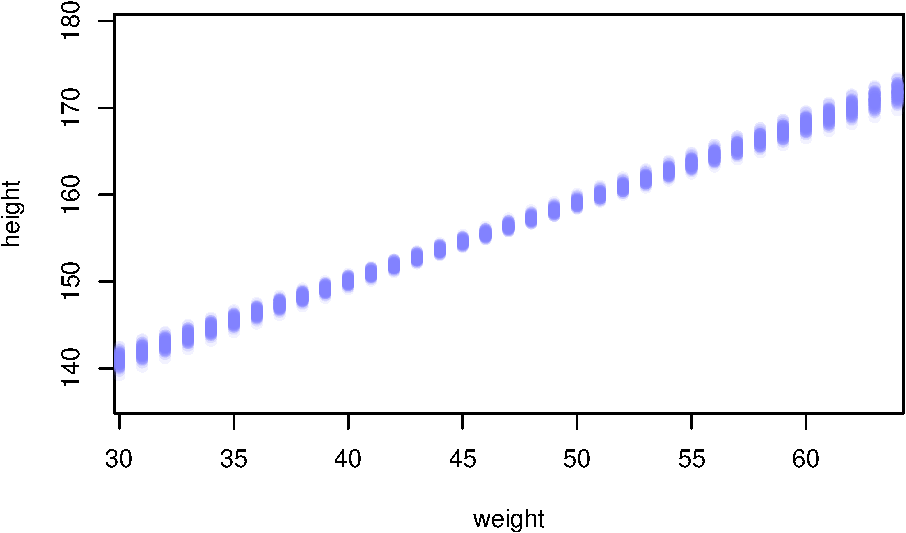
\includegraphics[keepaspectratio]{bookdown-demo_files/figure-latex/unnamed-chunk-29-1.pdf}}

The \texttt{link} function fixes the weight at the values in \texttt{weight.seq} and
draws samples from the posterior distribution of the parameters. We will do
the analog thing in the Frequentist framework.

We can also draw a nice shade for the regression line:

\begin{Shaded}
\begin{Highlighting}[]
\CommentTok{\# Summarize the distribution of mu}
\NormalTok{mu.mean }\OtherTok{\textless{}{-}} \FunctionTok{apply}\NormalTok{(mu, }\DecValTok{2}\NormalTok{, mean)}
\NormalTok{mu.PI }\OtherTok{\textless{}{-}} \FunctionTok{apply}\NormalTok{(mu, }\DecValTok{2}\NormalTok{, PI, }\AttributeTok{prob =} \FloatTok{0.89}\NormalTok{)}
\FunctionTok{plot}\NormalTok{(height }\SpecialCharTok{\textasciitilde{}}\NormalTok{ weight, d2, }\AttributeTok{col =} \FunctionTok{col.alpha}\NormalTok{(rangi2, }\FloatTok{0.5}\NormalTok{))}
\FunctionTok{lines}\NormalTok{(weight.seq, mu.mean)}
\FunctionTok{shade}\NormalTok{(mu.PI, weight.seq)}
\end{Highlighting}
\end{Shaded}

\pandocbounded{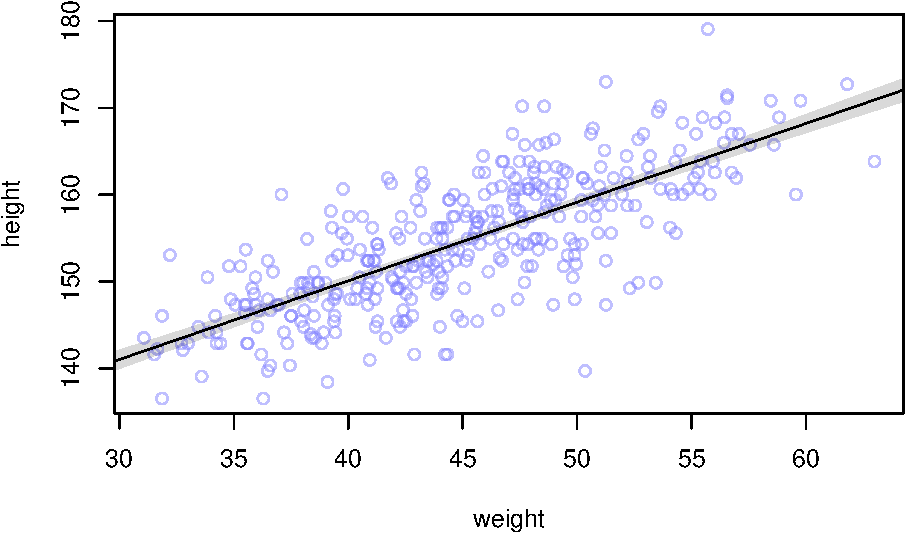
\includegraphics[keepaspectratio]{bookdown-demo_files/figure-latex/unnamed-chunk-30-1.pdf}}

The function \texttt{PI} from the \texttt{rethinking} package calculates the 89\% percentile interval
for the mean of the height at a certain weight. The \texttt{apply} function
apples this function to each columns (hence the \texttt{2}) of the matrix \texttt{mu}.

As we can see, we are pretty sure about the mean of height which
we wanted to model in the first place.

\textbf{Mean modeling is one thing, individual prediction is another}.
Given a certain weight of a person, what is the height of the same person?
The first line in the model definition (\(height_i \sim Normal(\mu_i, \sigma)\))
tells us that a person's height is distributed \emph{around} the mean
(which linearly depends on weight) and is not necessary the mean itself.

To get to an \textbf{individual prediction}, we need to consider the uncertainty
of the parameter estimation \emph{and} the uncertainty from the Gaussian distribution
around the mean (at a certain weight). We do this with \texttt{sim}.

\begin{Shaded}
\begin{Highlighting}[]
\CommentTok{\# Simulate heights from the posterior}
\NormalTok{sim.height }\OtherTok{\textless{}{-}} \FunctionTok{sim}\NormalTok{(mod, }\AttributeTok{data =} \FunctionTok{list}\NormalTok{(}\AttributeTok{weight =}\NormalTok{ weight.seq))}
\FunctionTok{str}\NormalTok{(sim.height)}
\end{Highlighting}
\end{Shaded}

\begin{verbatim}
##  num [1:1000, 1:46] 138 130 130 147 136 ...
\end{verbatim}

\begin{Shaded}
\begin{Highlighting}[]
\CommentTok{\# Compute the 89\% prediction interval for simulated heights}
\NormalTok{height.PI }\OtherTok{\textless{}{-}} \FunctionTok{apply}\NormalTok{(sim.height, }\DecValTok{2}\NormalTok{, PI, }\AttributeTok{prob =} \FloatTok{0.89}\NormalTok{)}

\CommentTok{\# Plot the raw data}
\FunctionTok{plot}\NormalTok{(height }\SpecialCharTok{\textasciitilde{}}\NormalTok{ weight, d2, }\AttributeTok{col =} \FunctionTok{col.alpha}\NormalTok{(rangi2, }\FloatTok{0.5}\NormalTok{))}

\CommentTok{\# Draw MAP (mean a posteriori) line}
\FunctionTok{lines}\NormalTok{(weight.seq, mu.mean)}

\CommentTok{\# Draw HPDI (highest posterior density interval) region for mu}
\FunctionTok{shade}\NormalTok{(mu.PI, weight.seq)}

\CommentTok{\# Draw PI (prediction interval) region for simulated heights}
\FunctionTok{shade}\NormalTok{(height.PI, weight.seq)}
\end{Highlighting}
\end{Shaded}

\pandocbounded{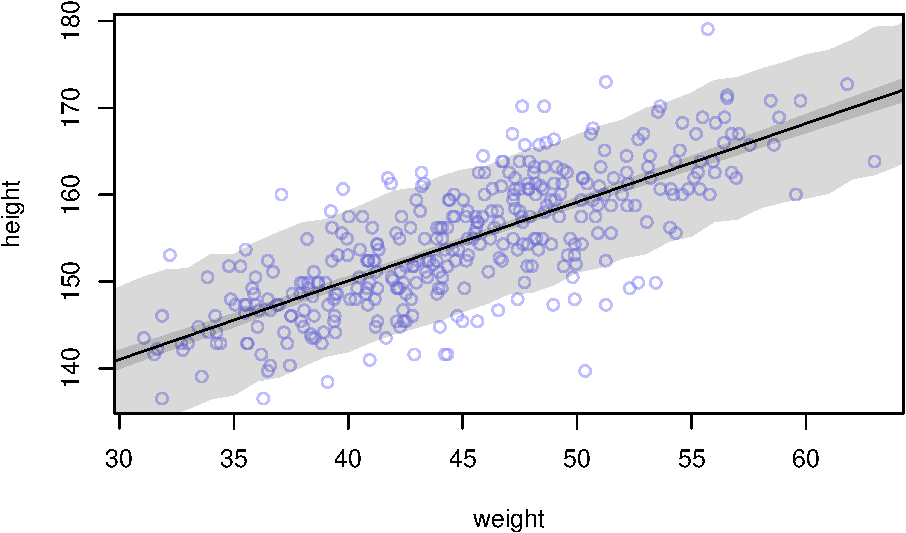
\includegraphics[keepaspectratio]{bookdown-demo_files/figure-latex/unnamed-chunk-31-1.pdf}}

Here, the \texttt{PI} function is applied to the simulated heights and calculates the 89\%
percentile interval for each weight.

The lighter and wider shaded region is where the model expects to find 89\%
of the heights of a person with a certain weight.

This part is \textbf{sometimes a bit desillusioning} when seen for the first time:
Draw a horizontal line at 150 cm and see how many weights (according to
the individual prediction) are compatible with this height. Weights
from 30 to 50 kg are compatible with this height according to the
89\% prediction interval:

\pandocbounded{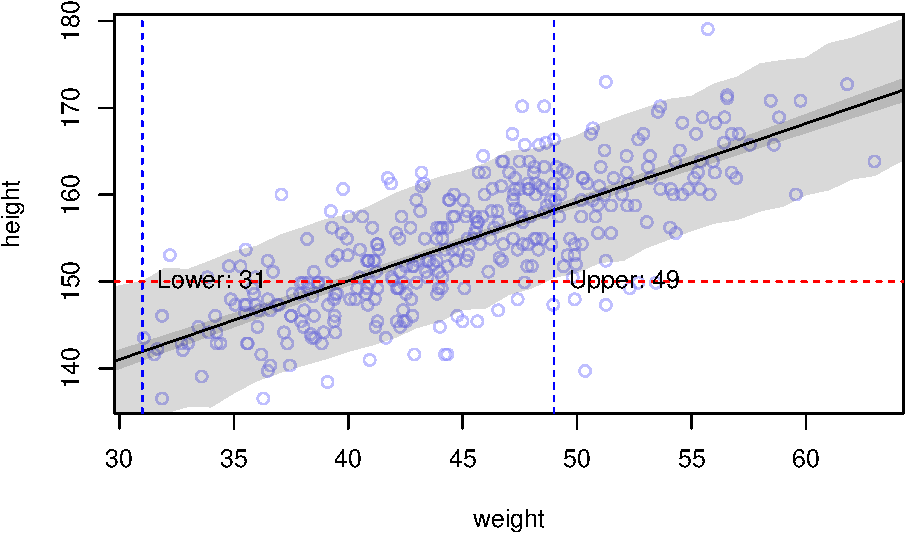
\includegraphics[keepaspectratio]{bookdown-demo_files/figure-latex/unnamed-chunk-32-1.pdf}}

The higher the credibility, the wider the interval,
the wider the range of compatible weights.
In our example, more than 60\% of the weight-range are
plausible to predict a height of 150 cm.

\begin{Shaded}
\begin{Highlighting}[]
\NormalTok{(}\DecValTok{50} \SpecialCharTok{{-}} \DecValTok{30}\NormalTok{) }\SpecialCharTok{/}\NormalTok{ (}\FunctionTok{range}\NormalTok{(d2}\SpecialCharTok{$}\NormalTok{weight)[}\DecValTok{2}\NormalTok{] }\SpecialCharTok{{-}} \FunctionTok{range}\NormalTok{(d2}\SpecialCharTok{$}\NormalTok{weight)[}\DecValTok{1}\NormalTok{])}
\end{Highlighting}
\end{Shaded}

\begin{verbatim}
## [1] 0.6265362
\end{verbatim}

On the other hand: We did not model the relationship this way.
We modeled \textbf{height depending on weight} and not the other way around.
In the next chapter, we will regress weight on height (yes, this is the correct order)
and see what changes.

\subsection{Summary}\label{summary}

\begin{itemize}
\tightlist
\item
  We have added a covariate (weight) to the simple mean model to predict height.
\item
  We have centered the weight variable.
\item
  We have defined and refined priors for the intercept and slope.
\item
  We have estimated the posterior distribution of the parameters using quadratic approximation with \texttt{quap}.
\item
  We have visualized the result.
\item
  We have created credible bands for mean and individual predictions.
\end{itemize}

\section{Simple Linear Regression in the Frequentist Framework}\label{simple-linear-regression-in-the-frequentist-framework}

We will now do the same analysis in the Frequentist framework while introducing
some foundational theory along the way.
I recommend reading the first couple of chapters from \href{https://www.routledge.com/Understanding-Regression-Analysis-A-Conditional-Distribution-Approach/Westfall-Arias/p/book/9780367493516?srsltid=AfmBOore3O_Ciecl0TTkr9AjPIY1d6OmbQa7o7IAdKpTSkD8s9HkwzD4}{Westfall}.

\subsection{Model definition}\label{model-definition-1}

Our linear model is defined as:

\[ h_i = \beta_0 + \beta_1 x_i + \varepsilon_i \]

where

\begin{itemize}
\tightlist
\item
  \(\varepsilon_i\) is the error term with \(\varepsilon_i \sim N(0, \sigma^2), \forall i\)
\item
  \(\beta_0\) is the unknown but fixed intercept
\item
  \(\beta_1\) is the unknown but fixed slope
\end{itemize}

\subsubsection{\texorpdfstring{Model Assumptions of the Classical Regression Model (\href{https://www.routledge.com/Understanding-Regression-Analysis-A-Conditional-Distribution-Approach/Westfall-Arias/p/book/9780367493516?srsltid=AfmBOore3O_Ciecl0TTkr9AjPIY1d6OmbQa7o7IAdKpTSkD8s9HkwzD4}{Westfall}, 1.7):}{Model Assumptions of the Classical Regression Model (Westfall, 1.7):}}\label{_model_assumptions}

The first and \textbf{most important assumption} is that the data are produced\\
probabilistically, which is specifically stated as
\[ Y|X = x \sim p(y|x)\]

What does this mean?

\begin{itemize}
\tightlist
\item
  \(Y|X = x\) is the random variable Y \textbf{conditional} on X being equal to x, i.e.~the
  distribution of \(Y\) if we know the value of \(X\) (in our example the weight in kg).
  \href{https://blogs.sas.com/content/iml/files/2015/09/GLM_normal_identity.png}{This} is a nice image of what is meant here.
\item
  \(p(y|x)\) is the distribution of potentially observable \(Y\) given \(X = x\).
  In our case above this was the normal distribution with mean \(\mu_i\) and variance \(\sigma\).
\end{itemize}

You can play with \href{https://psychmeth.shinyapps.io/Regression-NVFehler/}{this shiny app} to improve your understanding.
It offers the option ``Bedingte Verteilung anzeigen''.

One always thinks about the so-called
\href{https://en.wikipedia.org/wiki/Data_generating_process}{data generating process}
(\href{https://www.routledge.com/Understanding-Regression-Analysis-A-Conditional-Distribution-Approach/Westfall-Arias/p/book/9780367493516?srsltid=AfmBOore3O_Ciecl0TTkr9AjPIY1d6OmbQa7o7IAdKpTSkD8s9HkwzD4}{Westfall}, 1.2).
How did the data come about? There is a process behind it and this process
is attempted to be modeled.

\textbf{Further assumptions}:

\begin{itemize}
\item
  \textbf{Correct functional specification}: The conditional mean function \(f(x) = \mathbb{E}(Y|X=x)\).
  In the case of the linear model, the assumption is \(\mathbb{E}(Y|X=x) = \alpha + \beta x\).
  The \textbf{expectation} of \(Y\) (height) depends linearly on \(x\) (weight).
  This assumption is violated when the true relationship is not linear or the
  data at least suggest that it is not linear, like \href{https://www.alexanderdemos.org/Class5_files/figure-html/unnamed-chunk-2-1.png}{here}.
\item
  \textbf{The errors are homoscedastic} (constant variance \(\sigma^2\)). This means the
  variances of all conditional distributions \(p(y|x)\) are constant (\(=\sigma^2\)).
  This assumption is (for instance) violated if points are \href{https://www.investopedia.com/thmb/n9S9lWMv6X9-sKC2DtAOtUTPSik=/1500x0/filters:no_upscale():max_bytes(150000):strip_icc():format(webp)/Heteroskedasticity22-ce5acc2acef6494d91935588b0599579.png}{spreading out more and more
  around the regression line},
  indicating that the errors are getting larger.
\item
  \textbf{Normality}. For the classical linear regression model all the conditional
  distributions \(p(y|x)\) are normal distributions. It could well be, that
  the errors are not nicely normally distributed around the regression line,
  for instance if we have a lot of outliers upwards and the distribution
  is skewed, like \href{https://www.bookdown.org/rwnahhas/RMPH/mlr-normality.html}{here (Figure 5.20)}.
\item
  The \textbf{errors are independent} of each other.
  The potentially observable \(\varepsilon_i = Y_i - f(\mathbf{x_i}, \mathbf{\beta})\)
  is uncorrelated with \(\varepsilon_j = Y_j - f(\mathbf{x_j}, \mathbf{\beta})\) for
  \(i \neq j\). This assumption is violated if the errors are correlated,
  here is an example: The true data comes from a sine curve and we estimate a
  linear model (green), which does not fit the data well (left plot).
  The residuals plot shows clear patterns (right plot) and indicates
  that the errors are correlated. Specifically, the errors around \(x=2\) and \(x=4\)
  are negatively correlated (see \hyperref[exercise6_simpl_lin_reg]{exercise 6}).
\end{itemize}

\begin{verbatim}
## 
## Attaching package: 'patchwork'
\end{verbatim}

\begin{verbatim}
## The following object is masked from 'package:MASS':
## 
##     area
\end{verbatim}

\pandocbounded{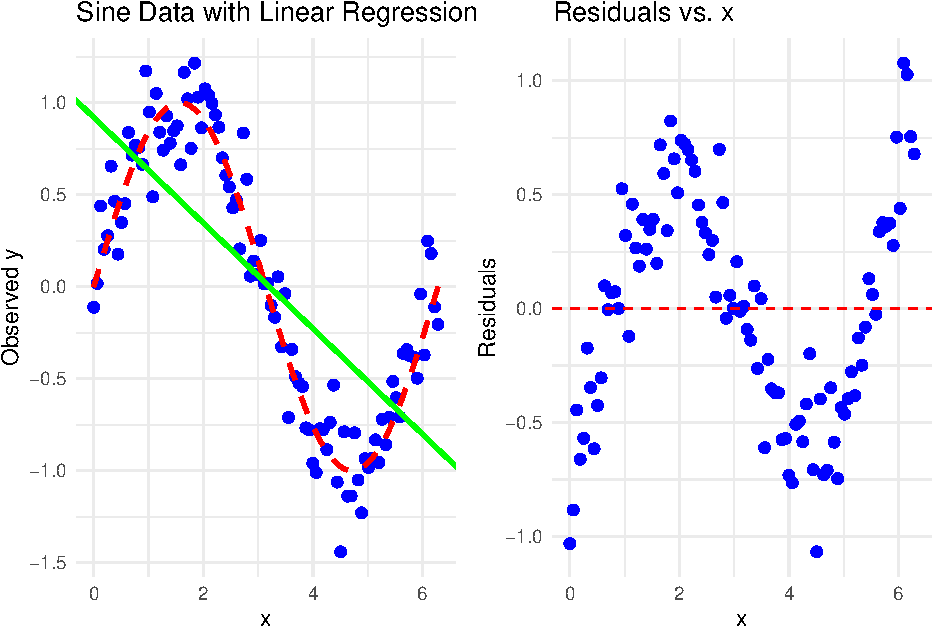
\includegraphics[keepaspectratio]{bookdown-demo_files/figure-latex/unnamed-chunk-34-1.pdf}}

In the case above, the errors are \textbf{not conditionally independent}.
If we condition on \(X=2\) and \(X=4.5\), the errors are correlated (\(r \sim -0.3\)),
which they should not be.

These assumptions become clearer as we go along and should be checked
for every model we fit. They are not connected, they can all be true or false.
The question is not ``Are the assumptions met?'' since they never are exactly met.
The question is \textbf{how} ``badly'' the assumptions are violated?

Remember, \textbf{all models are wrong, but some are useful}.

In full, the classical linear regression model can be written as:

\[ Y_i|X_i = x_i \sim_{independent} N(\beta_0 + \beta_1 x_{i1} + \dots \beta_k x_{ik},\sigma^2)\]
for \(i = 1, \dots, n\).

\subsection{Fit the model}\label{fit_model_simple_lin_reg_classic}

Again, we fit the model using the least squares method. For a neat animated explanation,
visit \href{https://www.youtube.com/watch?v=jEEJNz0RK4Q&ab_channel=COCCmath}{this video}.
There are literally hundreds of videos on the topic. Choose wisely. Not all are good.
If in doubt, use our recommended books as reading materials. This is the most reliable source.
A hint along the way: Be very sceptical if you ask GPT about information,
although for this special case one has a good chance of getting a decent answer due to
the vast amount of training data.

One has to minimize the sum of squared differences between the true heights and
the model-predicted heights in order to find \(\beta_0\) and \(\beta_1\).

\[ SSE(\beta_0, \beta_1) = \sum_{i=1}^n (y_i - (\beta_0 + \beta_1 x_i))^2 \]

We omit the technical details (set derivative to zero and solve the system) and give the results for \(\beta_0\) and \(\beta_1\):

\[
\hat{\beta_0} = \bar{y} - (\hat{\beta_1} \bar{x}),
\]
\[
\hat{\beta_1} = \frac{\sum_{i=1}^n (x_i - \bar{x})(y_i - \bar{y})}{\sum_{i=1}^n (x_i - \bar{x})^2} =
 \frac{s_{x,y}}{s_x^2} = r_{xy} \frac{s_y}{s_x}.
\]

where:

\begin{itemize}
\tightlist
\item
  \(r_{xy}\) is the \href{https://en.wikipedia.org/wiki/Pearson_correlation_coefficient}{sample correlation coefficient} between \(x\) and \(y\)
\item
  \(s_x\) and \(s_y\) are the \href{https://en.wikipedia.org/wiki/Standard_deviation}{uncorrected sample standard deviations} of \(x\) and \(y\)
\item
  \(s_x^2\) and \(s_{xy}\) are the \href{https://en.wikipedia.org/wiki/Variance}{sample variance} and \href{https://en.wikipedia.org/wiki/Covariance}{sample covariance}, respectively
\end{itemize}

Interpretation of \(\hat{\beta}_0\) and \(\hat{\beta}_1\): see \hyperref[exercise3_simpl_lin_reg]{exercise 3}.

Let's \textbf{use R again to solve the problem}:

\begin{Shaded}
\begin{Highlighting}[]
\FunctionTok{library}\NormalTok{(rethinking)}
\FunctionTok{data}\NormalTok{(Howell1)}
\NormalTok{d }\OtherTok{\textless{}{-}}\NormalTok{ Howell1}
\NormalTok{d2 }\OtherTok{\textless{}{-}}\NormalTok{ d[d}\SpecialCharTok{$}\NormalTok{age }\SpecialCharTok{\textgreater{}=} \DecValTok{18}\NormalTok{, ]}
\NormalTok{mod }\OtherTok{\textless{}{-}} \FunctionTok{lm}\NormalTok{(height }\SpecialCharTok{\textasciitilde{}}\NormalTok{ weight, }\AttributeTok{data =}\NormalTok{ d2)}
\FunctionTok{summary}\NormalTok{(mod)}
\end{Highlighting}
\end{Shaded}

\begin{verbatim}
## 
## Call:
## lm(formula = height ~ weight, data = d2)
## 
## Residuals:
##      Min       1Q   Median       3Q      Max 
## -19.7464  -2.8835   0.0222   3.1424  14.7744 
## 
## Coefficients:
##              Estimate Std. Error t value Pr(>|t|)    
## (Intercept) 113.87939    1.91107   59.59   <2e-16 ***
## weight        0.90503    0.04205   21.52   <2e-16 ***
## ---
## Signif. codes:  0 '***' 0.001 '**' 0.01 '*' 0.05 '.' 0.1 ' ' 1
## 
## Residual standard error: 5.086 on 350 degrees of freedom
## Multiple R-squared:  0.5696, Adjusted R-squared:  0.5684 
## F-statistic: 463.3 on 1 and 350 DF,  p-value: < 2.2e-16
\end{verbatim}

\textbf{Interpretation of R-output}:

\begin{itemize}
\tightlist
\item
  \texttt{Call}: The model that was fitted.
\item
  \texttt{Residuals}: \(r_i = height_i - \widehat{height}_i\).
  Differences between true heights and model-predicted heights.
\item
  \texttt{Coefficients}: Estimated for \(\beta_0\) and \(\beta_1\). We call them \(\hat{\beta}_0\) and \(\hat{\beta}_1\).

  \begin{itemize}
  \tightlist
  \item
    \texttt{Estimate}: The (least squares) estimated value of the coefficient.
  \item
    \texttt{Std.\ Error}: The standard error of the estimate.
  \item
    \texttt{t\ value}: The value of the \(t\)-statistic for the (Wald-) hypothesis test
    \(H_0: \beta_i = 0\).
  \item
    \texttt{Pr(\textgreater{}\textbar{}t\textbar{})}: The \(p\)-value of the hypothesis test.
  \end{itemize}
\item
  \texttt{Residual\ standard\ error}: The estimate of \(\sigma\)
  which is also a model parameter (as in the Bayesian framework).
\item
  \texttt{Multiple\ R-squared}: The proportion of the variance explained by the
  model (we will explain this below).
\item
  \texttt{Adjusted\ R-squared}: A corrected version of the \(R^2\) which takes into account
  the number of predictors in the model.
\item
  \texttt{F-statistic}: The value of the \(F\)-statistic for the hypothesis test:
  \(H_0: \beta_1 = \beta_2 = \dots = \beta_k = 0\). Note, the alternative
  hypotheses to this test is that \emph{any} of the \(\beta_i\) is not zero. If that is
  the case, the model explains more than the mean model with just \(\beta_0\).
\end{itemize}

We could also \textbf{solve the least squares problem graphically}: We want to find the
values of \(\beta_0\) and \(\beta_1\) that minimize the sum of squared differences
which can be plotted as 3D function. Since the function is a sum of squared terms,
we should expected a paraboloid form.
All we have to do is to ask R which of
the coordinates (\(\beta_0\), \(\beta_1\)) minimizes the sum of squared errors. The result confirmes
the results from the \texttt{lm} function. The dot in red marks the spot
(Code is in the \href{https://github.com/jdegenfellner/Script_QM2_ZHAW}{git repository}):

\textbf{---COMPILE CODE AT DEOPLOYMENT (takes a bit)---}

\begin{verbatim}
## Intercept beta_0:  113.8794
\end{verbatim}

\begin{verbatim}
## Slope beta_1:  0.9050291
\end{verbatim}

\begin{verbatim}
## file:////private/var/folders/pm/jd6n6gj10371_bml1gh8sc5w0000gn/T/RtmpOZ9C46/file5f901ef86f2f/widget5f90484b868b.html screenshot completed
\end{verbatim}

\pandocbounded{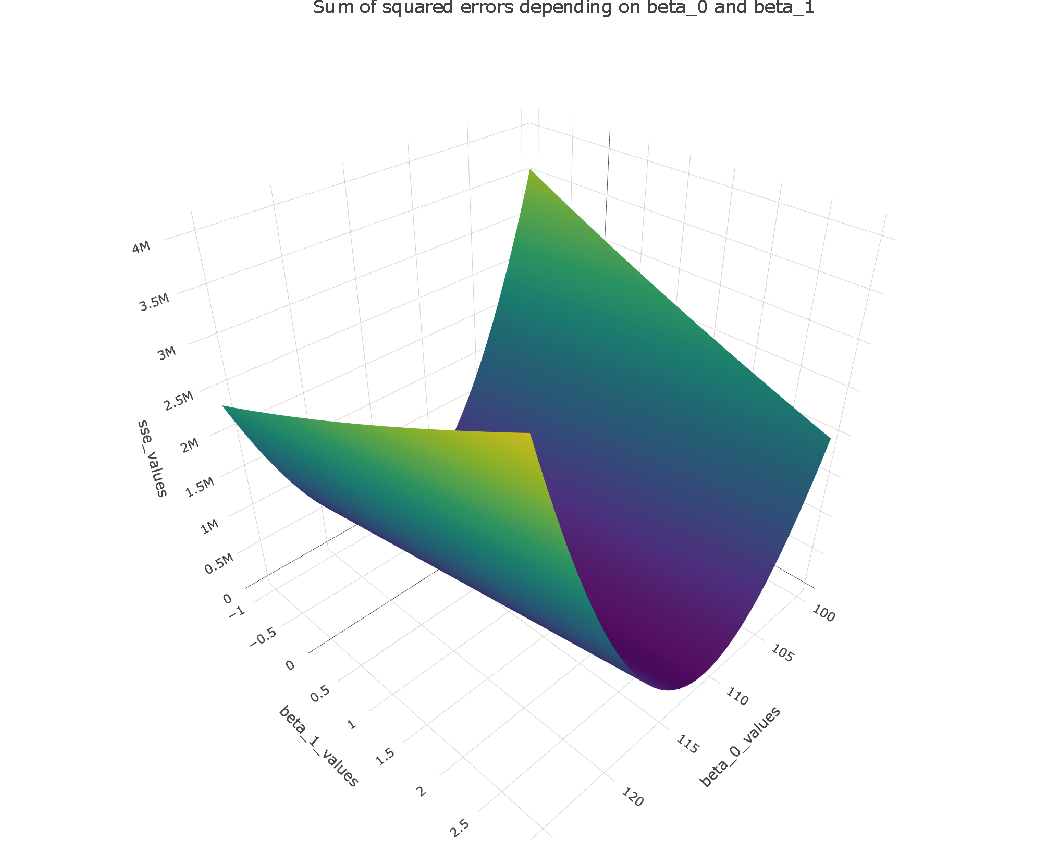
\includegraphics[keepaspectratio]{bookdown-demo_files/figure-latex/unnamed-chunk-36-1.pdf}}

\subsection{Confidence Intervals of coefficients (Frequentist)}\label{confidence_intervals_frequentist}

You can get CI's conveniently with the \texttt{confint} function:

\begin{Shaded}
\begin{Highlighting}[]
\FunctionTok{confint}\NormalTok{(mod, }\AttributeTok{level =} \FloatTok{0.96}\NormalTok{)}
\end{Highlighting}
\end{Shaded}

\begin{verbatim}
##                    2 %        98 %
## (Intercept) 109.939864 117.8189232
## x             0.818351   0.9917072
\end{verbatim}

Remember, these are Frequentist confidence intervals.

\textbf{If one repeats the experiment
many times, the true but unknown value of the parameter will
be in the interval in 96\% of the cases.}

We can also use the simple \href{https://en.wikipedia.org/wiki/Bootstrapping_(statistics)}{bootstrap}.
The advantage of this technique is that we can basically always use it,
no matter how compliated the estimator is. We do not need formulae.
We simply

\begin{itemize}
\tightlist
\item
  create 1000 bootstrap samples,
\item
  fit the model,
\item
  store the coefficients.
\item
  The 2\% and 98\% quantiles of the coefficients constitute the 96\% bootstrap confidence interval.
\end{itemize}

\begin{Shaded}
\begin{Highlighting}[]
\FunctionTok{set.seed}\NormalTok{(}\DecValTok{123}\NormalTok{)}
\NormalTok{n }\OtherTok{\textless{}{-}} \FunctionTok{nrow}\NormalTok{(d2)}
\NormalTok{B }\OtherTok{\textless{}{-}} \DecValTok{1000}
\NormalTok{boot\_coefs }\OtherTok{\textless{}{-}} \FunctionTok{matrix}\NormalTok{(}\ConstantTok{NA}\NormalTok{, }\AttributeTok{nrow =}\NormalTok{ B, }\AttributeTok{ncol =} \DecValTok{2}\NormalTok{)}
\ControlFlowTok{for}\NormalTok{ (i }\ControlFlowTok{in} \DecValTok{1}\SpecialCharTok{:}\NormalTok{B) \{}
\NormalTok{  boot\_idx }\OtherTok{\textless{}{-}} \FunctionTok{sample}\NormalTok{(}\DecValTok{1}\SpecialCharTok{:}\NormalTok{n, }\AttributeTok{replace =} \ConstantTok{TRUE}\NormalTok{)}
\NormalTok{  boot\_mod }\OtherTok{\textless{}{-}} \FunctionTok{lm}\NormalTok{(height }\SpecialCharTok{\textasciitilde{}}\NormalTok{ weight, }\AttributeTok{data =}\NormalTok{ d2[boot\_idx, ])}
\NormalTok{  boot\_coefs[i, ] }\OtherTok{\textless{}{-}} \FunctionTok{coef}\NormalTok{(boot\_mod)}
\NormalTok{\}}
\CommentTok{\#head(boot\_coefs)}
\FunctionTok{t}\NormalTok{(}\FunctionTok{apply}\NormalTok{(boot\_coefs, }\DecValTok{2}\NormalTok{, quantile, }\FunctionTok{c}\NormalTok{(}\FloatTok{0.02}\NormalTok{, }\FloatTok{0.98}\NormalTok{)))}
\end{Highlighting}
\end{Shaded}

\begin{verbatim}
##               2%         98%
## [1,] 110.1862455 117.4516455
## [2,]   0.8229982   0.9859997
\end{verbatim}

The CIs are quite similar to the ones from the \texttt{confint} function.

In the Bayesian setting, we used the centered weight variable. Let's to this here too for
comparison and use 89\% coverage probability.

\begin{Shaded}
\begin{Highlighting}[]
\NormalTok{d2}\SpecialCharTok{$}\NormalTok{weight\_centered }\OtherTok{\textless{}{-}}\NormalTok{ d2}\SpecialCharTok{$}\NormalTok{weight }\SpecialCharTok{{-}} \FunctionTok{mean}\NormalTok{(d2}\SpecialCharTok{$}\NormalTok{weight)}
\NormalTok{mod\_centered }\OtherTok{\textless{}{-}} \FunctionTok{lm}\NormalTok{(height }\SpecialCharTok{\textasciitilde{}}\NormalTok{ weight\_centered, }\AttributeTok{data =}\NormalTok{ d2)}
\CommentTok{\#summary(mod\_centered)}
\FunctionTok{confint}\NormalTok{(mod\_centered, }\AttributeTok{level =} \FloatTok{0.89}\NormalTok{)}
\end{Highlighting}
\end{Shaded}

\begin{verbatim}
##                      5.5 %      94.5 %
## (Intercept)     154.162715 155.0314698
## weight_centered   0.837658   0.9724002
\end{verbatim}

Compare with \texttt{precis} from the Bayesian model:

\begin{verbatim}
##              mean         sd       5.5%       94.5%
## a     154.5972131 0.27033041 154.165173 155.0292533
## b       0.9050133 0.04192753   0.838005   0.9720216
## sigma   5.0718667 0.19115317   4.766367   5.3773663
\end{verbatim}

We are glad to see that both analyses align really nicely.

\subsection{ANOVA (Analysis of Variance)}\label{analysis_of_variance}

A non-obvious and very useful finding is that the total variability (SST)
in the data (our heights) can be
\textbf{decomposed} (or \href{https://en.wiktionary.org/wiki/analysis}{analysed})
into two parts:

\begin{itemize}
\tightlist
\item
  The variability explained by the model (the regression line): SSR
\item
  The variability not explained by the model (the residuals): SSE
\end{itemize}

\[ \text{Sum of Squares in Total} = \text{Sum of Squares from Regression} + \text{Sum of Squared Errors} \]

\[ SST = SSR + SSE \]

\[ \sum_{i=1}^{n} (y_i - \bar{y})^2 = \sum_{i=1}^{n} (\hat{y}_i - \bar{y})^2 + \sum_{i=1}^{n} (y_i - \hat{y}_i)^2 \]

If you are interested in the details, check out \href{https://en.wikipedia.org/wiki/Explained_sum_of_squares\#Partitioning_in_the_general_ordinary_least_squares_model}{this}.

\href{https://www.youtube.com/watch?v=NxRTs7sXKAQ&ab_channel=365DataScience}{This video}
explains the concept nicely.

Let's visualize our regression result:

\begin{verbatim}
## `geom_smooth()` using formula = 'y ~ x'
\end{verbatim}

\pandocbounded{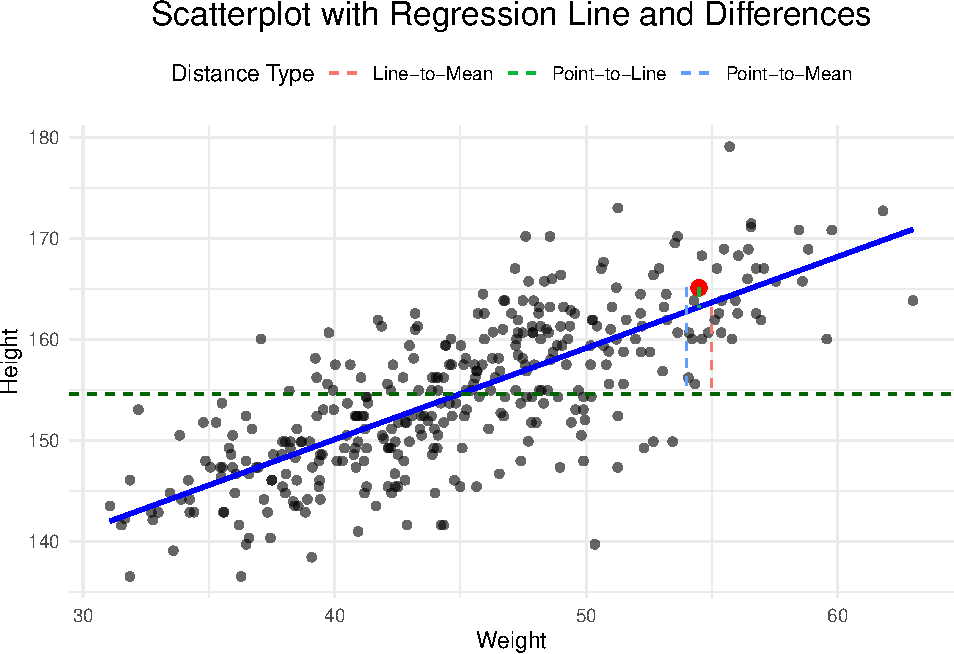
\includegraphics[keepaspectratio]{bookdown-demo_files/figure-latex/unnamed-chunk-41-1.pdf}}

The blue dotted line is the distance from
the mean to the point (total variance), the red dotted line is the distance from
the mean to the regression line (explained variance) and the green dotted line
is the distance from the regression line to the point (unexplained variance).
We see that it adds up. I find this fact quite fascinating.
One finds additivity by considering not determinisic values, but variances.
Thank you \href{https://en.wikipedia.org/wiki/Analysis_of_variance\#:~:text=ANOVA\%20was\%20developed\%20by\%20the,to\%20different\%20sources\%20of\%20variation.}{Ronald Fisher}.

See \hyperref[exercise13_simpl_lin_reg]{exercise 13}.

\subsection{\texorpdfstring{\(R^2\) - Coefficient of Determination}{R\^{}2 - Coefficient of Determination}}\label{r2---coefficient-of-determination}

\href{https://en.wikipedia.org/wiki/Coefficient_of_determination}{\(R^2\)}
is the \textbf{amount of variance explained by the model}.
You can also read \href{https://www.routledge.com/Understanding-Regression-Analysis-A-Conditional-Distribution-Approach/Westfall-Arias/p/book/9780367493516?srsltid=AfmBOore3O_Ciecl0TTkr9AjPIY1d6OmbQa7o7IAdKpTSkD8s9HkwzD4}{Westfall} 8.1.

As you can see
\hyperref[analysis_of_variance]{above}, the total variance (SST) of our outcome (height)
can be decomposed into two parts: the variance explained by the model (SSR)
and the variance not explained by the model (SSE).

Maybe the most intuitive definition of \(R^2\) is:

\[ R^2 = \frac{SSR}{SST} = \frac{SST - SSE}{SST} = 1 - \frac{SSE}{SST}\]

The value is between 0 and 1. The higher the value, the more variance is explained.
But be cautious. Depending on the context, a really high \(R^2\) is not
necessarily a good thing. With the data we are working with,
it could easily hint towards an error. If we are near 1,
all points in the simple linear regression model are on the line.
If we are near 0, the model does not explain much of the variance
and we would see ``noise with no slope'' in the scatterplot (\hyperref[exercise4_simpl_lin_reg]{exercise 4}).
The normal \(R^2\) can be found in the R output under \texttt{Multiple\ R-squared}.

If you add a lot of variables to your regression model, you can get an
\(R^2\) of 1. The \(R^2\) will never decrease when adding more variables.
We will verify this when we have more than 2 explanatory variables.
As a non-formal explanation for this: In the Sum of Squares Errors (SSE),
if you add more covariates (\(\beta_2, \beta_3\)), you have more freedom
to choose values that minimize the number that will be squared. Simple regression
is just a special case of multiple (more than one predictor) regression with \(\beta_2=\beta_3=\dots=0\).
Hence, you will definitely not be worse off with regards to SSE when using more covariates.
A smaller SSE implies a larger SSR (sum constraint; SST remains constant) and hence a larger \(R^2\).
If you have as many explanatory variables as data points, you can get an \(R^2\) of 1. This is
\href{https://en.wikipedia.org/wiki/Overfitting}{overfitting} at its ``best'' (which we want to avoid).
You would just get a value for each data point by setting all other \(\beta_i\) to zero and
\(\beta_i = \frac{y_i}{x_i}\).
Since we want to find the unterlying process, we want to avoid this.

Although not perfect, one way to mitigate the influence of ``too many'' variables
on \(R^2\) is to use the adjusted \(R^2\), which an also be found in the R output (\texttt{Adjusted\ R-squared}).

\subsubsection{\texorpdfstring{Seperating property of regression due to \(R^2\):}{Seperating property of regression due to R\^{}2:}}\label{seperating_property}

\href{https://www.routledge.com/Understanding-Regression-Analysis-A-Conditional-Distribution-Approach/Westfall-Arias/p/book/9780367493516?srsltid=AfmBOore3O_Ciecl0TTkr9AjPIY1d6OmbQa7o7IAdKpTSkD8s9HkwzD4}{Peter Westfall}
explains (in Figure 8.1 of the book) how \(R^2\) influences the separation of distributions in our simple regression model.

In our regression of \emph{height on weight} (the order is correct, that's how you say it),
the \(R^2\) is \(0.5696\). The following plot shows how ``well'' (i.e.~precise) one can predict
height if we use the 10\% and 90\% quantile of the weights (x\_low and x\_high).
In both, you see the conditional distribution of height given the weight \(X = x_{low}\) or \(X = x_{high}\).
Scenario 1 is the original model, scenario 2 is the same data with added noise (in Y-direction),
which reduces \(R^2\) to \(0.13\), much lower. In the right plot, the distributions have a large
overlap and it is hard to distinguish between weights when seeing the height.
With a very low \(R^2\), the height prediction does not really change and we could just as well
use the mean model.

\pandocbounded{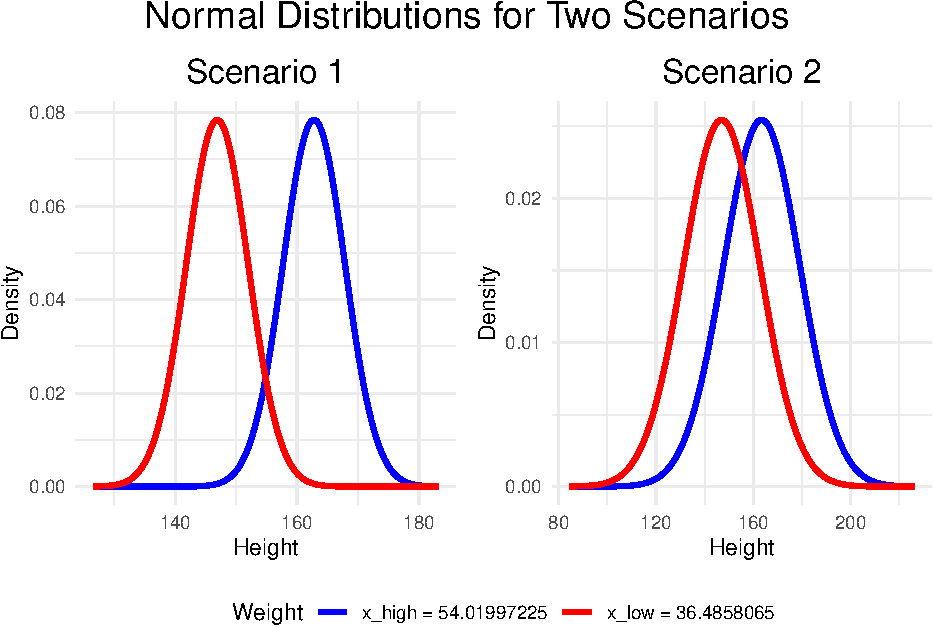
\includegraphics[keepaspectratio]{bookdown-demo_files/figure-latex/unnamed-chunk-42-1.pdf}}

In the left plot, given \(X = x_{low}\) gives a a rather strongly shifted normal distribution of
potentially observable heights for this weight compared to \(X=x_{high}\).
We would have a lower missclassification error when trying to distinguish heights
of very light and very heavy people in the sample just by seeing the height.
You can think of an even more extreme separation of these distributions,
which would happen, when \(R^2\) is very high or the true slope is much higher.

See also \hyperref[exercise5_simpl_lin_reg]{exercise 5}.

An interesting way to look at \(R^2\) is the following:
Given, that one person is in the 90\% quantile of the weight,
the other is in the 10\% quantile. What is the probability that the
height of the person in the 90\% quantile is higher than the height of the other person?
We could calculate this relatively easy using theorems about additivity of normal distributions.
Since we are all about application, we simulate this:

\begin{Shaded}
\begin{Highlighting}[]
\FunctionTok{library}\NormalTok{(rethinking)}
\FunctionTok{data}\NormalTok{(Howell1)}
\NormalTok{d }\OtherTok{\textless{}{-}}\NormalTok{ Howell1}
\NormalTok{d2 }\OtherTok{\textless{}{-}}\NormalTok{ d[d}\SpecialCharTok{$}\NormalTok{age }\SpecialCharTok{\textgreater{}=} \DecValTok{18}\NormalTok{, ]}
\CommentTok{\# Simulate heights for the two quantiles}
\NormalTok{n\_sims }\OtherTok{\textless{}{-}} \DecValTok{10000}
\FunctionTok{set.seed}\NormalTok{(}\DecValTok{123}\NormalTok{)}
\NormalTok{mod }\OtherTok{\textless{}{-}} \FunctionTok{lm}\NormalTok{(height }\SpecialCharTok{\textasciitilde{}}\NormalTok{ weight, }\AttributeTok{data =}\NormalTok{ d2)}
\FunctionTok{summary}\NormalTok{(mod)}\SpecialCharTok{$}\NormalTok{r.squared}
\end{Highlighting}
\end{Shaded}

\begin{verbatim}
## [1] 0.5696444
\end{verbatim}

\begin{Shaded}
\begin{Highlighting}[]
\NormalTok{x\_low\_high }\OtherTok{\textless{}{-}} \FunctionTok{quantile}\NormalTok{(d2}\SpecialCharTok{$}\NormalTok{weight, }\AttributeTok{probs =} \FunctionTok{c}\NormalTok{(}\FloatTok{0.1}\NormalTok{, }\FloatTok{0.9}\NormalTok{))}
\NormalTok{x\_low\_high}
\end{Highlighting}
\end{Shaded}

\begin{verbatim}
##      10%      90% 
## 36.48581 54.01997
\end{verbatim}

\begin{Shaded}
\begin{Highlighting}[]
\NormalTok{mean1 }\OtherTok{\textless{}{-}} \FloatTok{113.8793936} \SpecialCharTok{+} \FloatTok{0.9050291} \SpecialCharTok{*}\NormalTok{ x\_low\_high[}\DecValTok{1}\NormalTok{]}
\NormalTok{mean2 }\OtherTok{\textless{}{-}} \FloatTok{113.8793936} \SpecialCharTok{+} \FloatTok{0.9050291} \SpecialCharTok{*}\NormalTok{ x\_low\_high[}\DecValTok{2}\NormalTok{]}
\NormalTok{sd }\OtherTok{\textless{}{-}} \FloatTok{5.086}  \CommentTok{\# Standard deviation for both distributions}
\NormalTok{simulated\_heights }\OtherTok{\textless{}{-}} \FunctionTok{tibble}\NormalTok{(}
  \CommentTok{\# conditional normal distribution according to the model}
  \AttributeTok{low\_heights =} \FunctionTok{rnorm}\NormalTok{(n\_sims, }\AttributeTok{mean =}\NormalTok{ mean1, }\AttributeTok{sd =}\NormalTok{ sd),}
  \AttributeTok{high\_heights =} \FunctionTok{rnorm}\NormalTok{(n\_sims, }\AttributeTok{mean =}\NormalTok{  mean2, }\AttributeTok{sd =}\NormalTok{ sd)}
\NormalTok{)}

\CommentTok{\# Calculate the probability that the height of the person in the 90\% quantile is higher}
\CommentTok{\# than the height of the person in the 10\% quantile}
\NormalTok{simulated\_heights }\SpecialCharTok{\%\textgreater{}\%}
  \FunctionTok{mutate}\NormalTok{(}\AttributeTok{higher\_height =}\NormalTok{ high\_heights }\SpecialCharTok{\textgreater{}}\NormalTok{ low\_heights) }\SpecialCharTok{\%\textgreater{}\%}
\NormalTok{  dplyr}\SpecialCharTok{::}\FunctionTok{summarise}\NormalTok{(}\FunctionTok{mean}\NormalTok{(higher\_height))}
\end{Highlighting}
\end{Shaded}

\begin{verbatim}
## # A tibble: 1 x 1
##   `mean(higher_height)`
##                   <dbl>
## 1                 0.987
\end{verbatim}

In other words, we can be almost sure, that a person in the 90\% quantile of the weight
is taller than a person in the 10\% quantile of the weight given this data set.
See also \hyperref[exercise11_simpl_lin_reg]{exercise 11}.

\subsection{Check regression assumptions}\label{check-regression-assumptions}

Everytime we fit a model, we should check the assumptions \hyperref[_model_assumptions]{above}.
We do this for different reasons (which will become clearer over the course).
The assumptions are independent of each other.
They can all be true or false or some can be true and some false
(\href{https://www.routledge.com/Understanding-Regression-Analysis-A-Conditional-Distribution-Approach/Westfall-Arias/p/book/9780367493516?srsltid=AfmBOore3O_Ciecl0TTkr9AjPIY1d6OmbQa7o7IAdKpTSkD8s9HkwzD4}{Wesftall}, p.21).
Chapter 4 in the book is dedicated to this topic. It is important to know
that the assumptions are usually not met exactly. The question is \emph{how badly} they are violated,
not \emph{if} they are violated.
Furthermore, the asssumptions refer to the data generating process, not the data itself.
Thus, the evaluation of the assumptions should involve subject matter knowledge.

\(p\)-values to evaluate model assumptions are not a good idea. To \href{https://www.tandfonline.com/doi/full/10.1080/00031305.2016.1154108\#d1e949}{quote} the
American Statistical Association (ASA): ``By itself, a \(p\)-value does not provide a good measure
of evidence regarding a model or hypothesis.''
Deicision-tree thinking might not be the best idea for statistical modeling.

We will not use hypothesis tests for assumptions, because

\begin{itemize}
\tightlist
\item
  They are never met exactly. You cannot ``prove'' them.
\item
  With small sample sizes, the statistical \emph{power} is often low.
\item
  With large sample sizes, the smallest deviation will be ``significant''.
\end{itemize}

We will follow the book (chapter 4, pages 99ff) and use graphical and simulation methods to check the assumptions.
As guidance, we could check them in the following order:

\begin{itemize}
\tightlist
\item
  Linearity
\item
  Constant variance
\item
  Independence
\item
  Normality
\end{itemize}

\subsubsection{Linearity}\label{linearity}

First, we \textbf{plot the data}, as we did already above. We can add a
a smoothing line to the raw data as well:

\begin{verbatim}
## `geom_smooth()` using formula = 'y ~ x'
\end{verbatim}

\pandocbounded{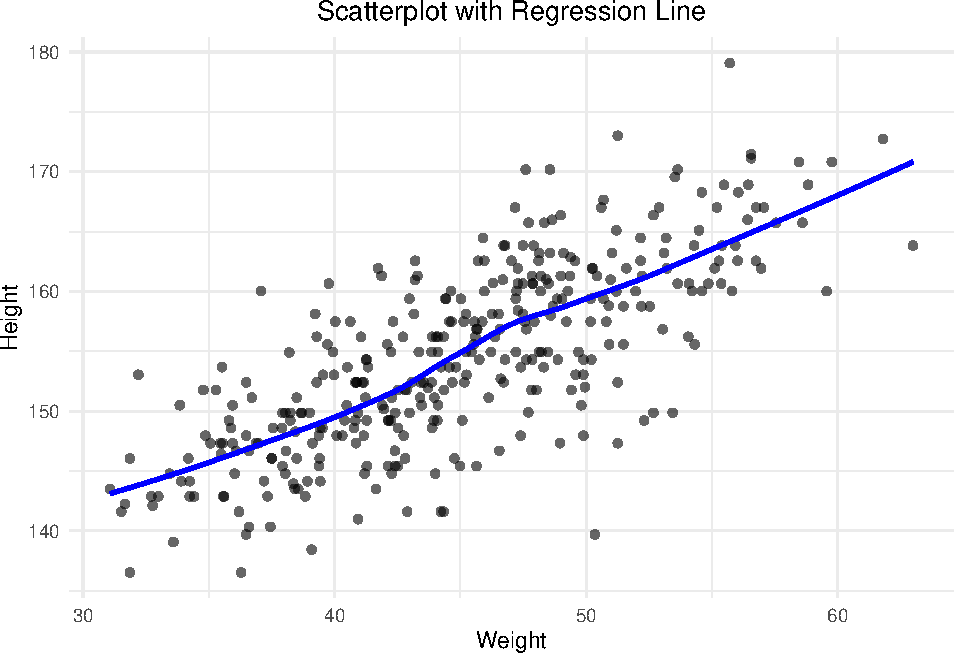
\includegraphics[keepaspectratio]{bookdown-demo_files/figure-latex/unnamed-chunk-44-1.pdf}}

It looks like this relationship is describable in a linear way.
No apparent curvature or patches.
A refined version of the scatterplot of the raw data is The
\textbf{residual scatter plot} (\(x_i, e_i\)):

\begin{verbatim}
## `geom_smooth()` using formula = 'y ~ x'
\end{verbatim}

\pandocbounded{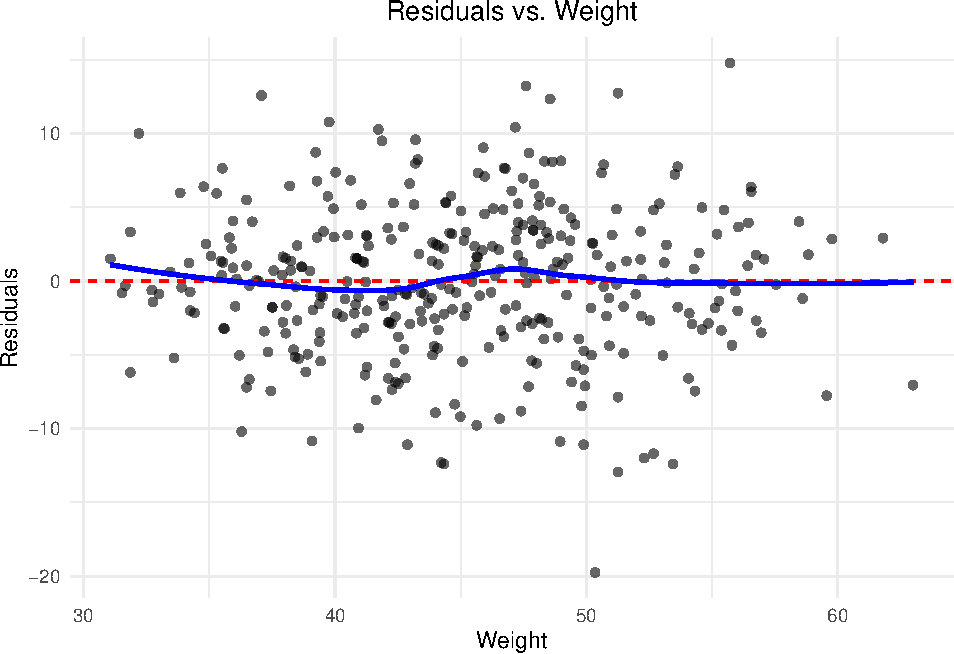
\includegraphics[keepaspectratio]{bookdown-demo_files/figure-latex/unnamed-chunk-45-1.pdf}}

Compared to the scatterplot above, the residuals plot magnifies
possible curvature. The reason is that the range of residuals
is smaller than the range of the heights.

In multiple regression, we will use the (\(\hat{y_i}, e_i\)) plot, which is
identical to the plot above in simple linear regression, but
very helpful in multiple regression.
You get the (\(\hat{y_i}, e_i\)) plot in R with \texttt{plot(mod,\ which\ =\ 1)}.

\subsubsection{Constant variance}\label{constant_variance}

This assumption means that the variance of the residuals is constant.
If it is violated, the spread around a hypothetical regression line is not constant.
We look at the residual scatter plot again:

\pandocbounded{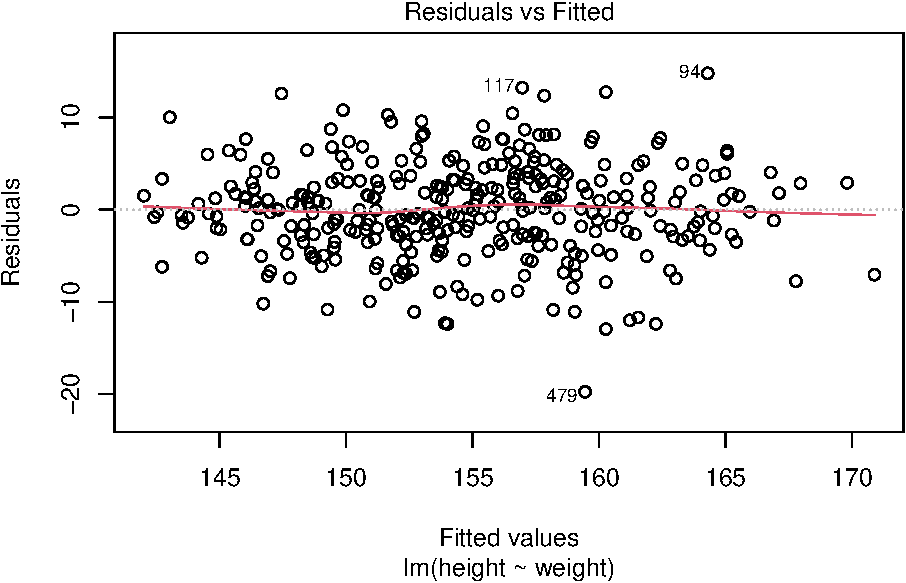
\includegraphics[keepaspectratio]{bookdown-demo_files/figure-latex/unnamed-chunk-46-1.pdf}}

Look for a changes in patterns of vertical variability. Note, that you
often do not have as many data points near the end of the range of the predictor.
Here are some examples of heteroskedasticity:
\href{https://i0.wp.com/statisticsbyjim.com/wp-content/uploads/2017/08/residuals_unfixed.png?resize=576\%2C384}{1},
\href{https://encrypted-tbn0.gstatic.com/images?q=tbn:ANd9GcQPAPMGV5U0Pe0nKnhoZWHJ8KypqVCls6ZQZud84C3KM8SJqOkuMNeJl2oTg-UDuukJRhk&usqp=CAU}{2},
\href{https://i.sstatic.net/R5KIH.png}{3}.
The above looks homoscedastic. If it was heteroskedastic, this is not a problem,
we just have to model it differently (later).

As always, it is a good idea to study the variability of these plots
using simulation (\hyperref[exercise7_simpl_lin_reg]{exercise 7}).

Better for detecting heteroscedasticity is the (\(\hat{y_i}, |e_i|\)) plot
with a smoothing line:

\begin{verbatim}
## 'data.frame':    544 obs. of  4 variables:
##  $ height: num  152 140 137 157 145 ...
##  $ weight: num  47.8 36.5 31.9 53 41.3 ...
##  $ age   : num  63 63 65 41 51 35 32 27 19 54 ...
##  $ male  : int  1 0 0 1 0 1 0 1 0 1 ...
\end{verbatim}

\begin{verbatim}
## `geom_smooth()` using formula = 'y ~ x'
\end{verbatim}

\pandocbounded{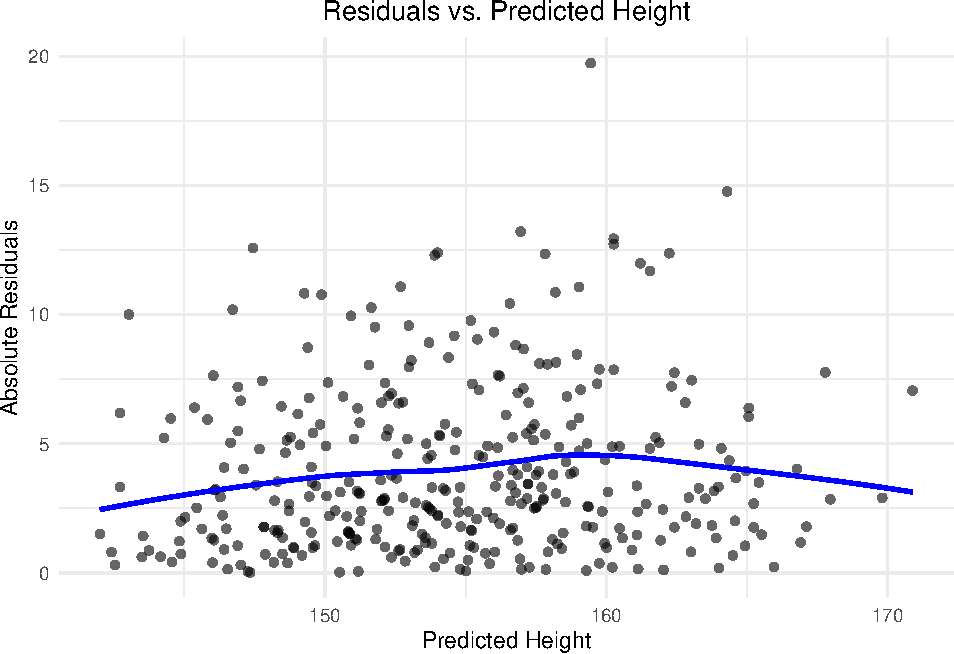
\includegraphics[keepaspectratio]{bookdown-demo_files/figure-latex/unnamed-chunk-47-1.pdf}}

This will probably not be a perfectly horizontal line, since
there are less points at the end of the range of the predictor.
For instance, There are less people with extreme weights in the data set.

\subsubsection{Independence, uncorrelated errors}\label{independence-uncorrelated-errors}

We had an example above, where the errors were correlated.
The sine curve could stem from time series data, where the \(x\)-variable
is the time and the \(y\)-variable is a seasonally changing variable
like temperature (purely hypothetical). In \hyperref[exercise6_simpl_lin_reg]{exercise 6},
the values are autocorrelated: Correlated with previous values of the same variable.
If we would track the body heights of persons over time, we would have
an autocorrelated time series since the height of a person at time \(t\) is
correlated with the height of the same person at time \(t-1\), but a little
less with the height at time \(t-2\) and so on. If I am tall today, it is
very likely that I was tall yesterday.

In our case of the !Kung San data, we do not have autocorrelated data.

But still, we could look at the correlations the residuals with lagged residuals.
A \(lag=1\) means I compare the residuals with the ones right next to me and check if
they are correlated.

\begin{verbatim}
## cor= 0.01858044
\end{verbatim}

\pandocbounded{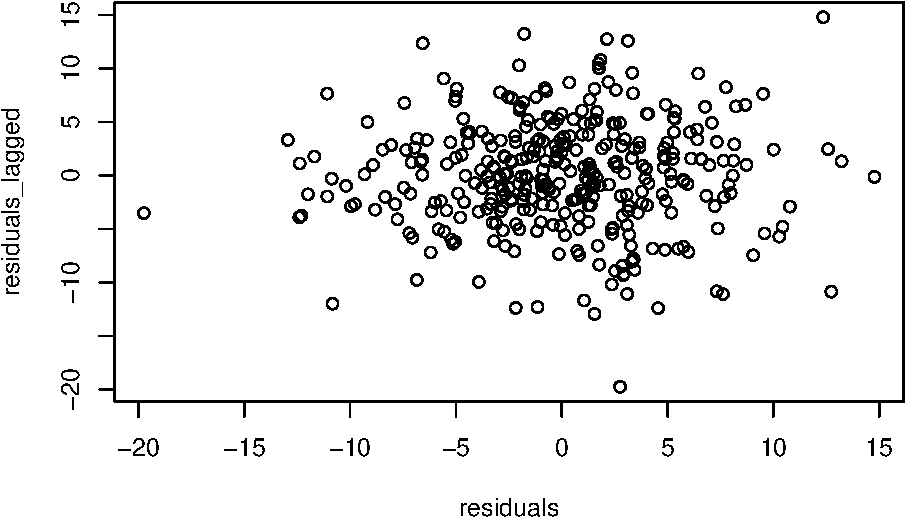
\includegraphics[keepaspectratio]{bookdown-demo_files/figure-latex/unnamed-chunk-48-1.pdf}}

It least with a lag of \(1\), there so no large correlation between the residuals.

\subsubsection{Normality}\label{normality_assumption}

This assumptions states that the conditional distribution \(Y|X=x\)
is a normal distribution. We do not look at the normality of \(Y\) itself,
since it is not a formal requirement, that \(Y\) is normally distributed.
We need to assess the normality of the residuals \[e_i = y_i - \hat{y}_i\]
I like doing this with a \href{https://jdegenfellner.github.io/Script_QM1_ZHAW/descriptive_stats.html\#q-q-plots}{Q-Q plot}
from the R package \texttt{car} (command \texttt{qqPlot}):

\begin{verbatim}
## Loading required package: carData
\end{verbatim}

\begin{verbatim}
## 
## Attaching package: 'car'
\end{verbatim}

\begin{verbatim}
## The following object is masked from 'package:dplyr':
## 
##     recode
\end{verbatim}

\begin{verbatim}
## The following object is masked from 'package:purrr':
## 
##     some
\end{verbatim}

\begin{verbatim}
## The following object is masked from 'package:rethinking':
## 
##     logit
\end{verbatim}

\pandocbounded{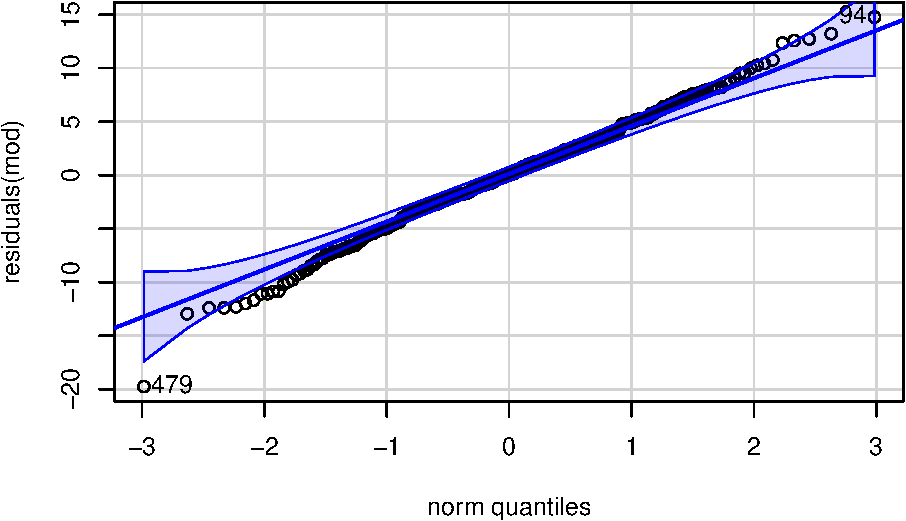
\includegraphics[keepaspectratio]{bookdown-demo_files/figure-latex/unnamed-chunk-49-1.pdf}}

\begin{verbatim}
## 479  94 
## 317  72
\end{verbatim}

With the 97\% confidence envelope, we can see if the residuals are
consistent with coming from a normal distribution.
We could again use simulation to see how the Q-Q Plot changes
to get a better feeling (see \hyperref[exercise9_simpl_lin_reg]{exercise 9}).

Another convenient way to check model assumptions (for a wide class of models)
is to use the \texttt{check\_model} function from the \texttt{performance} package:

\pandocbounded{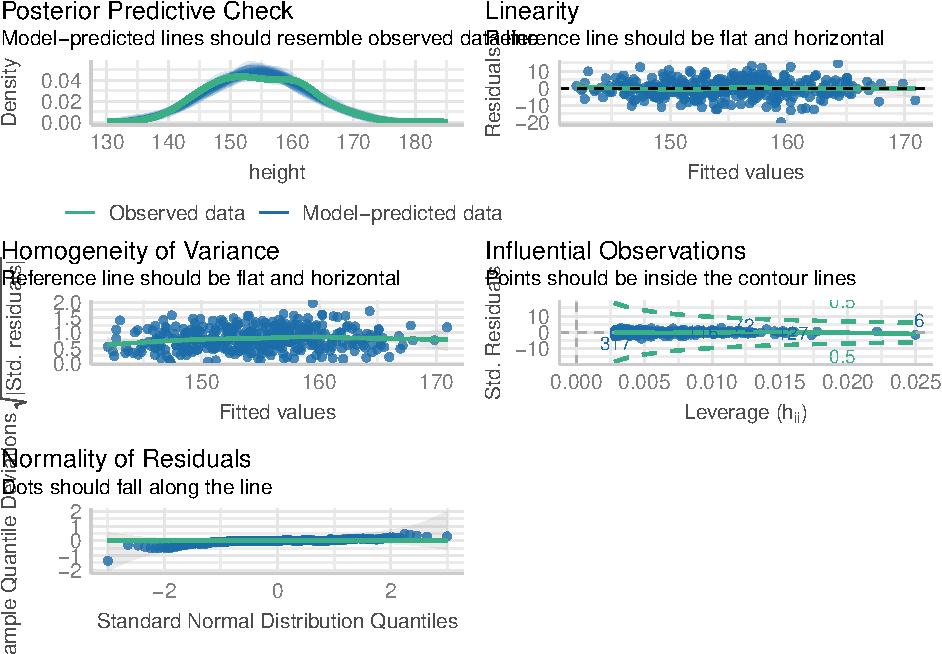
\includegraphics[keepaspectratio]{bookdown-demo_files/figure-latex/unnamed-chunk-50-1.pdf}}

In this case, everything looks fine. Let's go through the plots and explain them one by one:

\paragraph{Posterior predictive check (upper left)}\label{posterior-predictive-check-upper-left}

Here, you create new data from the estimated model. We did that already in
the Bayesian framework using \texttt{sim} from the \texttt{rethinking} package.
You could also try the command \texttt{extract.samples()}from the \texttt{rethinking} package
(Statistical Rethinking p.~196) to create
new data from the Frequentist model. You can try this in our exercises sessions.
Using least squares, the estimated model was:
\[ height_i = 113.87939 + 0.90503 \cdot weight_i + Normal(0, 5.086) \]
From this model, we can simulate new data (or the original weights, if we want to use fixed X)
by plugging in different weights, and adding a random error from a normal distribution
with mean 0 and standard deviation 5.086.
Then, we can compare the distribution of the simulated data with the observed data.
The blue lines in the graph are model predicted heights, the green line are the
observed heights.

Let's try to replicate this plot.
First, we want to simulate new data from the model.
A scatter plot is also a nice way to check of the model predictions
are in line with the observed data. One could repeat this process
multiple times to get a feeling for the variability of the model predictions.

\begin{verbatim}
## `geom_smooth()` using formula = 'y ~ x'
\end{verbatim}

\pandocbounded{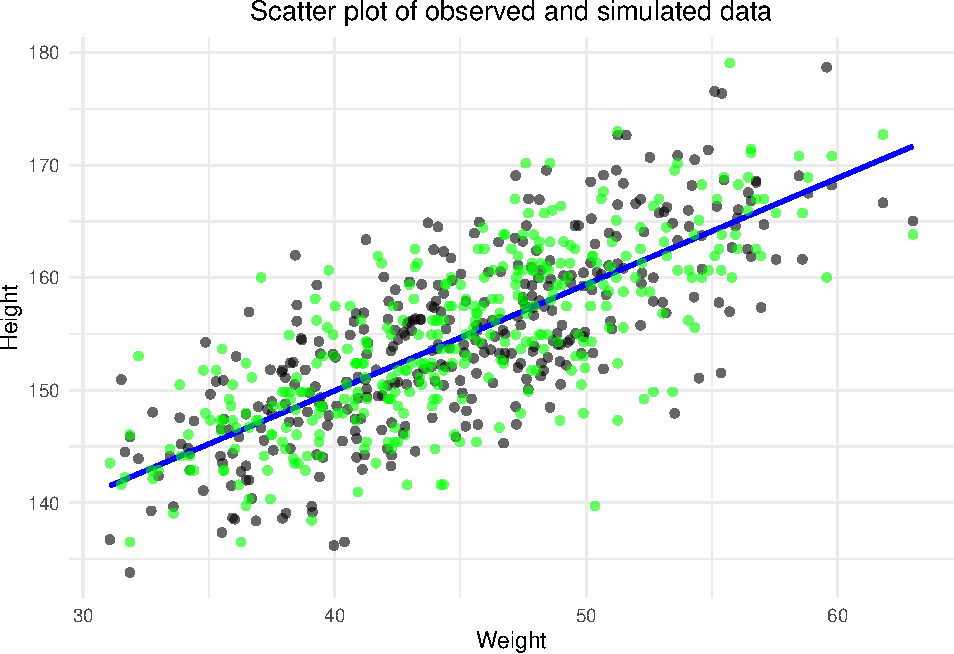
\includegraphics[keepaspectratio]{bookdown-demo_files/figure-latex/unnamed-chunk-51-1.pdf}}

The simulated and original data (green) fit nicely together.
This lends some credibility to the model - at least in terms of prediction.
And now the density plots of the model created data (blue) and the observed data (green):

\pandocbounded{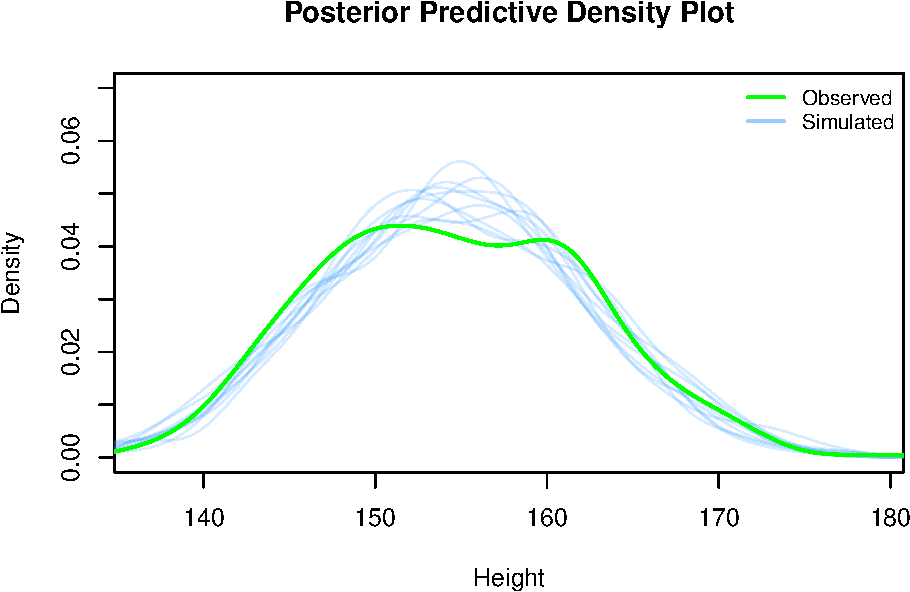
\includegraphics[keepaspectratio]{bookdown-demo_files/figure-latex/unnamed-chunk-52-1.pdf}}

As you can see, the densities of the observed and simulated data are broadly similar.
One could argue that heights in the range of 150-160 cm are a bit overestimated by the model.
Depending on the context, this might be a problem or not. Let's accept the model for now.

\paragraph{Linear fit (upper right)}\label{linear-fit-upper-right}

This is the same plot as \hyperref[linearity]{above}: \((\hat{y}_i, e_i)\).

\paragraph{Homogeneity of variance (middle left)}\label{homogeneity-of-variance-middle-left}

This is the same plot as \hyperref[constant_variance]{above}: \((\hat{y}_i, |e_i|)\).

\paragraph{Influential observations (middle right)}\label{influential-observations-middle-right}

The standard method to check for influential observations is to compute the
so-called \href{https://en.wikipedia.org/wiki/Cook\%27s_distance}{Cook's distance}.
This is a measure of how much leverage a single observation has on the model.
We can extract the Cook's distance from the model using \texttt{cooks.distance()}.
An ugly rule of thumb would be to look at observations with a Cook's distance
greater than 1.
In the plot, the leverage \(h_{ii}\) is on the x-axis, and the standardized residuals
are on the y-axis. In short, a high leverage means that the estimated value \(\hat{y}_i\)
is potentially far away from the original value \(y_i\).
The contours (dotted green lines) are the Cook's distance, in this
case at a Cook's distance of 0.5.
There is \href{https://en.wikipedia.org/wiki/Cook\%27s_distance\#Relationship_to_other_influence_measures_(and_interpretation)}{formula}
that relates the leverage (\(h_{ii}\)), the Cook's distance
and the residuals. Holding Cook`s distant constant at 0.5,
gives you the green dotted line in the plot.

Let's create an outlier and see what happens:

\pandocbounded{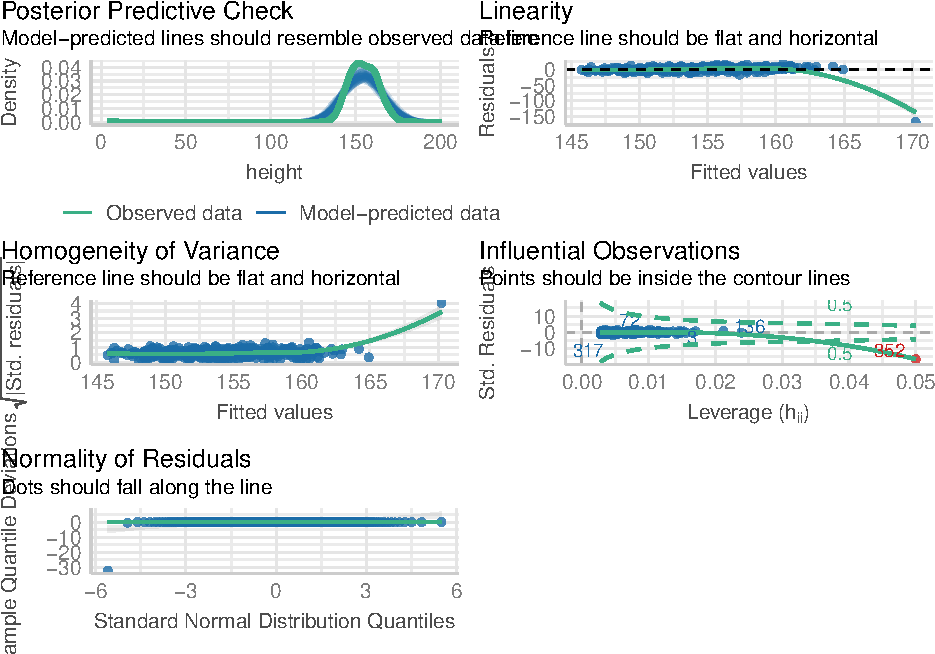
\includegraphics[keepaspectratio]{bookdown-demo_files/figure-latex/unnamed-chunk-53-1.pdf}}

\begin{verbatim}
## `geom_smooth()` using formula = 'y ~ x'
\end{verbatim}

\pandocbounded{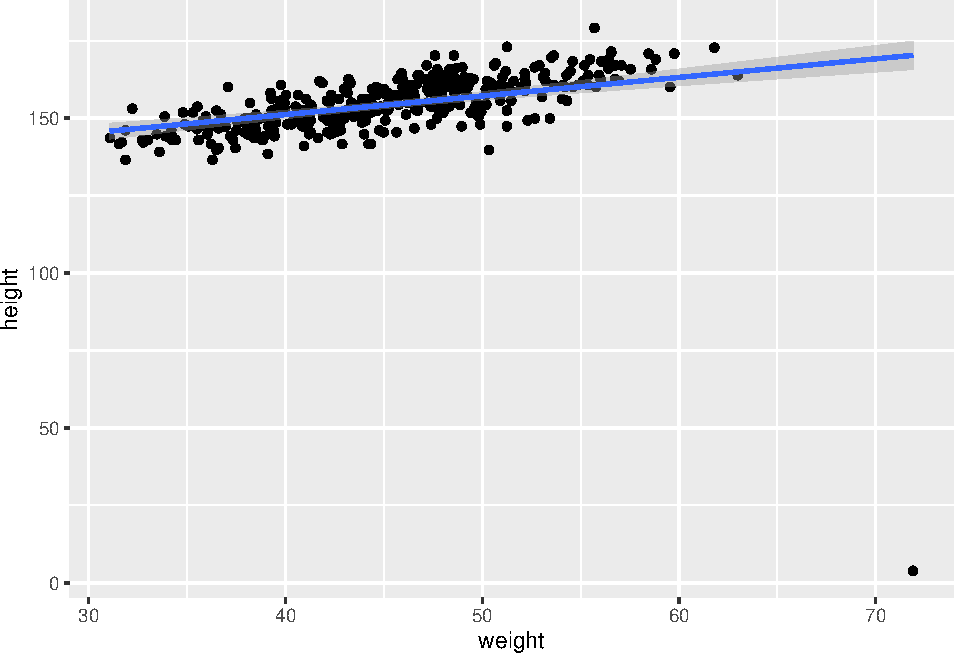
\includegraphics[keepaspectratio]{bookdown-demo_files/figure-latex/unnamed-chunk-53-2.pdf}}

\begin{verbatim}
## Cook's distance =  7.025207
\end{verbatim}

One single outlier changes the diagnostic plots. Observation 352
is clearly identified as influential. The one point
changes all diagnostic plots notably.
The estimates of the regression coefficients
are also affected:

\begin{verbatim}
## [1] "Original Model"
\end{verbatim}

\begin{verbatim}
## (Intercept)      weight 
## 113.8793936   0.9050291
\end{verbatim}

\begin{verbatim}
## [1] "Model with outlier"
\end{verbatim}

\begin{verbatim}
## (Intercept)      weight 
##  127.172494    0.599054
\end{verbatim}

Admitted, this is a somewhat artificial example.

\paragraph{Normality of residuals (lower left)}\label{normality-of-residuals-lower-left}

This is basically the same plot as above, just \href{https://cran.r-project.org/web/packages/qqplotr/vignettes/introduction.html}{detrended}.
Let's try to replicate it:

\begin{verbatim}
## 
## Attaching package: 'qqplotr'
\end{verbatim}

\begin{verbatim}
## The following objects are masked from 'package:ggplot2':
## 
##     stat_qq_line, StatQqLine
\end{verbatim}

\pandocbounded{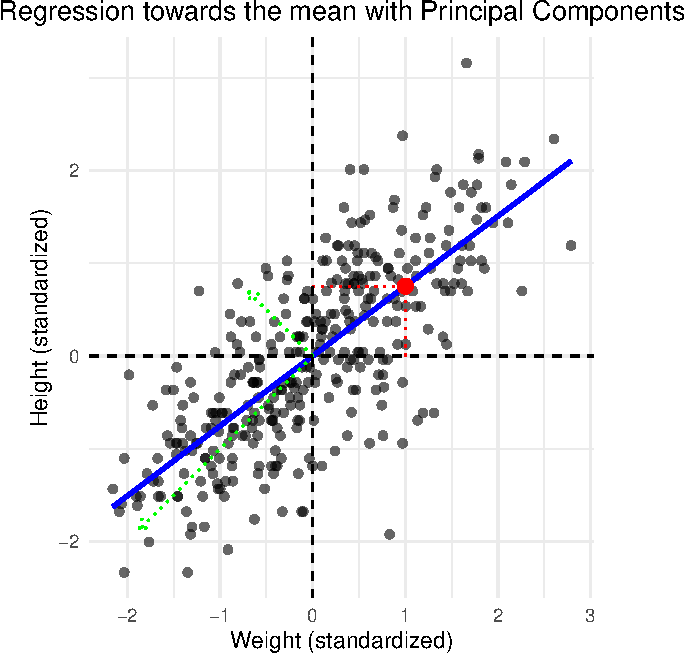
\includegraphics[keepaspectratio]{bookdown-demo_files/figure-latex/unnamed-chunk-55-1.pdf}}

The normality assumption seems to hold. Note that in the above QQ plot,
we detrended the residuals and used a bootrap confidence band. Depending
on the band type, the confidence band can be wider or narrower and include
or exclude points.

\textbf{After having checked the assumptions for the classical regression model}
and we feel comfortable with the model, we get exact confidence intervals
for the effect sizes (\(\beta\)s) using \texttt{confint()} (p.~74 in Westfall).

Heureka! We have a model that fits the data well.

\subsection{Bootstrap fit}\label{bootstrap-fit}

In order to get a feeling for the variability of the model with regards to the predictors as well,
we can bootstrap the whole data set, fit the model and draw regression lines.
We create \(100\) bootrap replicates of our data set \texttt{d2} by drawing with
replication. For every bootstrap replicate, we fit the model and draw the regression line.

\pandocbounded{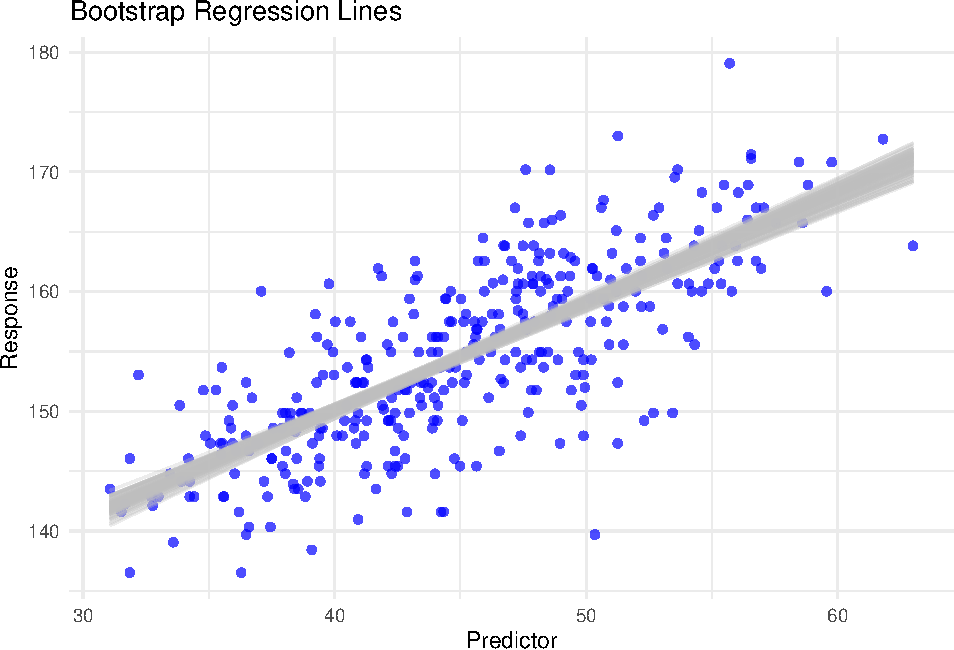
\includegraphics[keepaspectratio]{bookdown-demo_files/figure-latex/unnamed-chunk-56-1.pdf}}

The results is very stable. Neither intercept nor slope change much.

\subsection{Regression towards the mean}\label{regression-towards-the-mean}

There are great explanations for ``\href{https://en.wikipedia.org/wiki/Regression_toward_the_mean}{regression towards the mean}'' in
\href{http://www.stat.columbia.edu/~gelman/arm/}{Gelman} p.58 and
\href{https://www.routledge.com/Understanding-Regression-Analysis-A-Conditional-Distribution-Approach/Westfall-Arias/p/book/9780367493516?srsltid=AfmBOore3O_Ciecl0TTkr9AjPIY1d6OmbQa7o7IAdKpTSkD8s9HkwzD4}{Westfall} p.36.
This \href{https://www.youtube.com/watch?v=1tSqSMOyNFE&ab_channel=Veritasium}{video} might be interesting to watch.

It describes the phenomenon that the predicted value (y) is closer to its
mean than the predictor (x) to its mean.
In our case this means, if the weight of a person is 1 standard deviation above the mean of body weights,
the (model-)predicted height is less than 1 standard deviation above the mean of body heights, but
still larger than the average height. Let's verify:

\begin{verbatim}
## predicted height= 0.7547479
\end{verbatim}

\begin{verbatim}
## `geom_smooth()` using formula = 'y ~ x'
\end{verbatim}

\pandocbounded{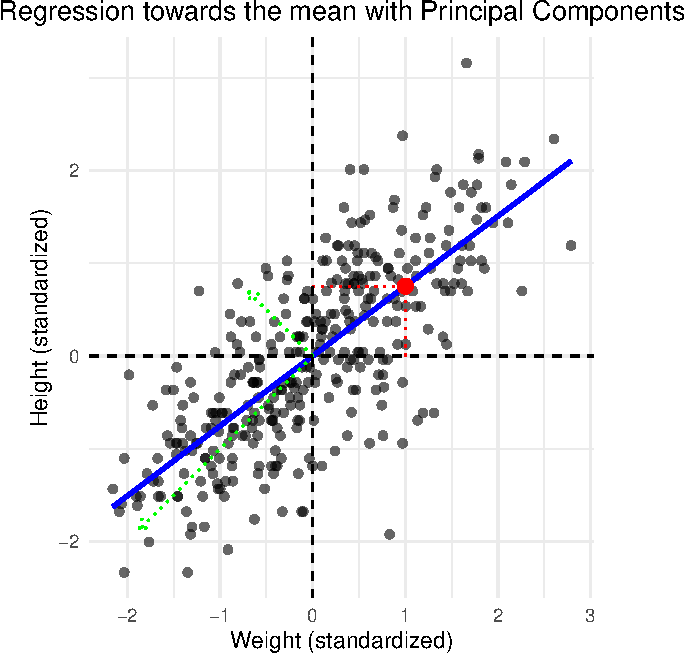
\includegraphics[keepaspectratio]{bookdown-demo_files/figure-latex/unnamed-chunk-57-1.pdf}}

As Gelman points out in his book (Figure 4.2), there is a fine detail:
The regression line is not the line most people would draw through the data.
They would draw a line through the main directions of variability
(directions are the eigenvectors of the covariance matrix).
In dotted green, you can see these directions. The regression line is a solution
to another problem (as we have seen): It minimizes the sum of squared residuals,
which are defined via the \textbf{vertical} distances to the line.
See \hyperref[exercise8_simpl_lin_reg]{exercise 8}.

\subsection{Random X vs.~fixed X}\label{random-x-vs.-fixed-x}

A detail that is not mentioned often in introductory statistics courses
is the question of whether the predictor variable \(X\) is random or fixed.
In our case, we did not specify the weights of the people in the !Kung San data set.
\emph{Obervational} data was collected and we have no control over the weights.
In an \emph{experimental} setting, we could have controlled the weights of the people.
We could have for instance only included people with weights at certain steps (50 kg, 60 kg, 70 kg).
In the latter case, we could consider X as fixed. In the former case, we consider X as random.
If we would draw another sample from the population, we would get different weights again.
Further reading: \href{https://www.routledge.com/Understanding-Regression-Analysis-A-Conditional-Distribution-Approach/Westfall-Arias/p/book/9780367493516?srsltid=AfmBOore3O_Ciecl0TTkr9AjPIY1d6OmbQa7o7IAdKpTSkD8s9HkwzD4}{Westfall} 1.5.

There are many more details we could look into, but we wanted to give a first
practical introduction to regression analysis with less emphasis on theory and proofs behind it.

We want to make clear what the confidence intervals from \texttt{confint} of a model mean. For this see
\hyperref[exercise14_simpl_lin_reg]{exercise 14}.

\section{Exercises}\label{exercises-1}

{[}E{]} Easy, {[}M{]} Medium, {[}H{]} Hard

(Some) solutions to exercises can be found in the git-repo \href{https://github.com/jdegenfellner/Script_QM2_ZHAW/tree/main/Solutions_Exercises}{here}.

\subsection{{[}E{]} Exercise 1}\label{exercise1_simpl_lin_reg}

In the model from above:

\begin{eqnarray*}
h_i &\sim& \text{Normal}(\mu_i, \sigma)\\
\mu_i &\sim& \alpha + \beta (x_i - \bar{x})\\
\alpha &\sim& \text{Normal}(171.1, 20)\\
\beta &\sim& \text{Normal}(0, 10)\\
\sigma &\sim& \text{Uniform}(0, 50)
\end{eqnarray*}

\begin{itemize}
\tightlist
\item
  What ist the expected height when \(x_i = \bar{x}\)?
\item
  What is the expected height when \(x_i\) changes by 1 unit?
\end{itemize}

\subsection{{[}E{]} Exercise 2}\label{exercise2_simpl_lin_reg}

Look at the marginal distrubutions of the parameters in the Bayesian model.

\begin{itemize}
\tightlist
\item
  Plot the posterior distribution of all 3 parameters.
\item
  Include in the plot a 99\% credible interval (HDI).
\end{itemize}

\subsection{{[}M{]} Exercise 3}\label{exercise3_simpl_lin_reg}

Go to the coefficient estimates in the simple linear regression setting
above (\hyperref[fit_model_simple_lin_reg_classic]{Fit the model})
in the classical framework.

\begin{itemize}
\tightlist
\item
  Create an R file to simulate the simple linear regression model.
\item
  Change your input parameters and see how the estimates change.
\item
  Does this make sense with respect to the estimates given, specifically with respect
  to \(\beta_1\)?
\end{itemize}

\subsection{{[}H{]} Exercise 4}\label{exercise4_simpl_lin_reg}

Verify the statement above in the text for high and low values of \(R^2\).

\subsection{{[}M{]} Exercise 5}\label{exercise5_simpl_lin_reg}

Verify with simulation in R that the separation of the distributions in the simple linear regression model
improves if the true (but usually unknown) slope increases.

\subsection{{[}H{]} Exercise 6}\label{exercise6_simpl_lin_reg}

Go to the model assumptions in the classical regression model (\hyperref[_model_assumptions]{Model Assumptions}).
- Use the code from \href{https://github.com/jdegenfellner/Script_QM2_ZHAW/blob/main/02-Simple_Linear_Regression.Rmd}{github}
to recreate the regression model with the sine-curve.
- Check the independence assumption as described. Look at the residuals, when \(X=2\) and \(X=4.5\).
You can get those by filtering residuals that are \(>0.5\) and \(<0.5\).

\subsection{{[}M{]} Exercise 7}\label{exercise7_simpl_lin_reg}

\begin{itemize}
\tightlist
\item
  Simulate data from the regression of heights on weights in our !Kung San data set.
\item
  Draw the \(\hat{y_i}, e_i\) plot.
\item
  Draw the \(\hat{y_i}, |e_i|\) plot.
\item
  Repeat the simulation and look at the variability of the plot.
\end{itemize}

\subsection{{[}E{]} Exercise 8}\label{exercise8_simpl_lin_reg}

\begin{itemize}
\tightlist
\item
  Go to p.36 in Westfall's book and read Appendix A.
\item
  Pay close attention to the explanation about regression toward the mean.
\end{itemize}

\subsection{{[}M{]} Exercise 9}\label{exercise9_simpl_lin_reg}

Go to the resuials \hyperref[normality_assumption]{above} where we tested the normality assumption.

\begin{itemize}
\tightlist
\item
  Calcuate mean and standard deviation from the residuals of the model
  that regresses height on weight.
\item
  Simulate from a normal distribution using these parameters.
\item
  Get a feeling how the QQ plot changes by drawing the QQ plot repeatedly.
\end{itemize}

\subsection{{[}M{]} Exercise 10}\label{exercise10_simpl_lin_reg}

Using our !Kung San data,

\begin{itemize}
\tightlist
\item
  show that the regression of height on weight (\texttt{lm(height\ \textasciitilde{}\ weight)})
  is not the same as the regression of weight on height (\texttt{lm(weight\ \textasciitilde{}\ height)}).
\item
  Draw both regression lines in one diagram.
\item
  Can you simulate data where the two regressions deliver (almost) identical results?
\item
  Explain why the results differ and what consequences this would have for a research question.
  Which question do I answer with each?
\end{itemize}

\subsection{{[}E{]} Exercise 11}\label{exercise11_simpl_lin_reg}

Go back to the \hyperref[seperating_property]{section} about \(R^2\) and the separation of the distributions.
How would the probability that a person in the 90\% quantile of the weight
is taller than a person in the 10\% quantile of the weight change if you change

\begin{itemize}
\tightlist
\item
  the true slope of the regression line
\item
  the true \(\sigma\), i.e.~if you add more noise and have a lower \(R^2\)?
\end{itemize}

\subsection{{[}M{]} Exercise 12}\label{exercise12_simpl_lin_reg}

Go back to the Bayesian simple regression model for height \hyperref[simple_lin_reg_bayes]{above}.

\begin{itemize}
\tightlist
\item
  Standardize weights and heights in the data set \texttt{d2}.
\item
  Estimate the regression model as we did in the section using \texttt{quap}.
\item
  Plot the posterior distribution using \texttt{plot(model)}.
\item
  Interpret the regression coefficient \(\beta\).
\end{itemize}

\subsection{{[}M{]} Exercise 13}\label{exercise13_simpl_lin_reg}

Go back to the \hyperref[analysis_of_variance]{ANOVA section}.

\begin{itemize}
\item
  Calculate SSE, SST and SSR for the regression of height on weight.
\item
  How many degrees of freedom does each term have?
\end{itemize}

\subsection{{[}M{]} Exercise 14}\label{exercise14_simpl_lin_reg}

When we fit a simple linear regression model (Frequentist), we get confidence intervals for the coefficients
using the command \texttt{confint}. As stated previously, these are Frequentist CIs. That means,
if we draw data from the true (but usually unknown) data generating process, we would expect
that the true value of the coefficient (intercept and slope) lies in the CI in X\% of the cases.

\begin{itemize}
\tightlist
\item
  Simulate data from the true data generating process of the simple linear regression model.
\item
  Fit the model and get the confidence intervals for the coefficients.
\item
  Repeat this process 1000 times and see how many times the true value of the coefficients
  lies in the CI.
\end{itemize}

Changing the distribution of the covariate \(x\) should not change the results, since
we only get a different amount of data points agross the range of \(x\).

\begin{itemize}
\tightlist
\item
  Verify this statement by changing the distribution of \(x\).
\end{itemize}

\section{eLearning 1}\label{elearning-1}

eLearning Assignments:

\begin{itemize}
\tightlist
\item
  Review all content from the script, up to and including section 3.1.
\item
  Reading assignment on frequentist statistics (exam-relevant!):
  Chapter 1 (Introduction to Regression Models) from the book
  Understanding Regression Analysis - A Conditional Distribution Approach.
\item
  Research task: Find at least two scientific articles in your field that apply
  regression (either simple regression with one predictor or multiple regression).
  We have already searched for journals relevant to your field in QM1.
  If you send me one of these studies in advance, we could also discuss the
  applied methods in more detail during the practice sessions.
\end{itemize}

\chapter{Multiple Linear Regression}\label{multiple-linear-regression}

So far, we have dealt with the simple mean model and the model with one predictor
in the Bayesian and Frequentist framework.
We will now add another predictor and subsequently an interaction term to the model.
Finally, we will add more than two predictors to the model.

If you feel confused at any point: As Richard McElreath repeatedly says:
This is normal, it means you are paying attention. I also refer to the
great \href{https://www.youtube.com/watch?v=lytxafTXg6c&ab_channel=sdfhsfh}{Richard Feynman}.

\section{Linear Regression with 2 predictors in the Bayesian Framework}\label{linear-regression-with-2-predictors-in-the-bayesian-framework}

\subsection{Meaning of ``linear''}\label{meaning-of-linear}

What is a linear model? The term ``linear'' refers to the relationship of the predictors
with the dependent variable (or outcome). The following model is also linear:

\[height_i = \beta_0 + \beta_1 x_i + \beta_2 x_i^2\]

The model is linear in the parameters \(\beta_0, \beta_1, \beta_2\) but not in the predictors \(x_i\).
The term \(x_i^2\) is ok, since the heights are just sums of multiples of the predictors (which can be nonlinear).
This model is not a linear model anymore:

\[height_i = \beta_0 + \beta_1 x_i + e^{\beta_2 x_i^2}\]

\(\beta_2\) is now is the exponent of \(e\). It would also not be linear,
if the coefficients are in a square root or in the denominator of a fraction,
or in a sine or in a logarithm. You get the idea.

Here is an easy way to check if the model is linear: If I change the predictor-value
(i.e.,the value of \(x_i\), \(x_i^2\) or whatever your predictor is) by one unit,
the change in the (expected value of the) dependent variable is the coefficient in front of
the predictor (\(\beta_i\)).

\subsection{Adding a transformed predictor to the model}\label{adding_transformed_predictor_bayes}

Around 4.5. in the book \href{https://civil.colorado.edu/~balajir/CVEN6833/bayes-resources/RM-StatRethink-Bayes.pdf}{Statistical Rethinking}
there is are lineare regression using a quadratic term for weight.
It is a principle, called the ``\textbf{variable inclusion principle}'', that we always include the lower order terms when fitting a model
with higher order terms. See \href{https://vdoc.pub/documents/understanding-regression-analysis-a-conditional-distribution-approach-84oqjr8sqva0}{Westfall},
p.~213. If we do not include the lower order terms, the coefficient does not measure what
we want it to meausure (curvature in our case). For instance, if we want to model a quadratic relationship (parabola) between
weight and height, we also have to include the linear term for weight (\(x_i\)).
Since we do not assume the relationship between weight and height to be linear but
quadratic (which is a polynomial of degree 2), we call this a
\href{https://en.wikipedia.org/wiki/Polynomial_regression\#:~:text=In\%20statistics\%2C\%20polynomial\%20regression\%20is,nth\%20degree\%20polynomial\%20in\%20x.}{polynomial regression}.
This \href{https://www.youtube.com/watch?v=QptI-vDle8Y&ab_channel=MikeXCohen}{video} could be instructive.
One has to be careful with fitting polynomials to data points since the regression coefficients
can become quite large. Using a polynomial of high degree implies to have a lot of parameters
to estimate. Increasing the degree of the polynomial increases \(R^2\) but also the risk of overfitting.
(see Statistical Rethinking p.~200). So this is - of course - not the final solution to regression problems.

This time, lets look at the whole age range of data from the !Kung San people.

\begin{Shaded}
\begin{Highlighting}[]
\FunctionTok{library}\NormalTok{(rethinking)}
\FunctionTok{library}\NormalTok{(tidyverse)}
\FunctionTok{data}\NormalTok{(Howell1)}
\NormalTok{d }\OtherTok{\textless{}{-}}\NormalTok{ Howell1}
\NormalTok{d }\SpecialCharTok{\%\textgreater{}\%} \FunctionTok{ggplot}\NormalTok{(}\FunctionTok{aes}\NormalTok{(}\AttributeTok{x =}\NormalTok{ weight, }\AttributeTok{y =}\NormalTok{ height)) }\SpecialCharTok{+}
  \FunctionTok{geom\_point}\NormalTok{() }\SpecialCharTok{+}
  \FunctionTok{geom\_smooth}\NormalTok{(}\AttributeTok{method =} \StringTok{"lm"}\NormalTok{, }\AttributeTok{se =} \ConstantTok{FALSE}\NormalTok{, }\AttributeTok{color =} \StringTok{"blue"}\NormalTok{) }\SpecialCharTok{+}
  \FunctionTok{geom\_smooth}\NormalTok{(}\AttributeTok{method =} \StringTok{"loess"}\NormalTok{, }\AttributeTok{se =} \ConstantTok{FALSE}\NormalTok{, }\AttributeTok{color =} \StringTok{"red"}\NormalTok{)}
\end{Highlighting}
\end{Shaded}

\begin{verbatim}
## `geom_smooth()` using formula = 'y ~ x'
## `geom_smooth()` using formula = 'y ~ x'
\end{verbatim}

\pandocbounded{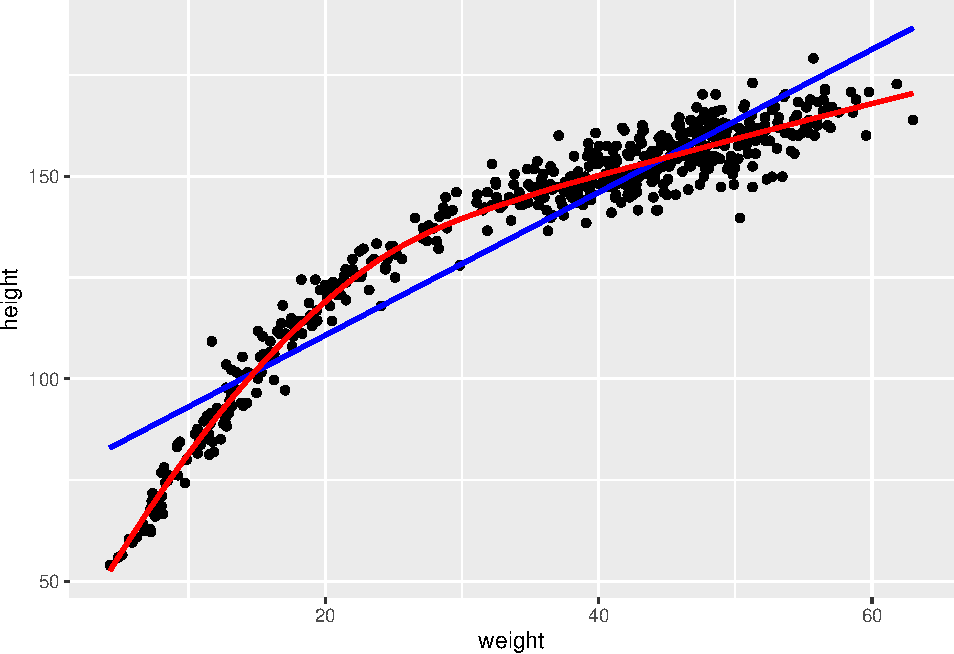
\includegraphics[keepaspectratio]{bookdown-demo_files/figure-latex/unnamed-chunk-58-1.pdf}}

It would not be a good idea to fit a linear trend through this data,
because we would not caupture the relationship adequately.
The red line is a \href{https://en.wikipedia.org/wiki/Local_regression}{loess smothing} line
which is often used to capture non-linear relationships.
The blue line is the usual line from classic linear regression (from the previous chapter).
Which one describes the data more accurately?
In this case it is obvious, a non-linear relationship is present and it might be a good idea
to model it. Modeling the relationship with a linear trend leads to bad residuals with structure.
We will demonstrate this in the freuqentist setting.
Unfortunately, in more complex settings, with more predictors, it is not always so easy to see.

This time, we use the mean for the prior from the book (\(178 cm\)).
The model equations are (see \hyperref[exercise2_multiple_regression]{exercise 2}):

\begin{eqnarray*}
h_i &\sim& \text{Normal}(\mu_i, \sigma) \\
\mu_i &=& \alpha + \beta_1 x_i + \beta_2 x_i^2 \\
\alpha &\sim& \text{Normal}(178, 20) \\
\beta_1 &\sim& \text{Log-Normal}(0, 1) \\
\beta_2 &\sim& \text{Normal}(0, 1) \\
\sigma &\sim& \text{Uniform}(0, 50)
\end{eqnarray*}

The prior for \(\beta_1\) is log-normal, because we can reasonably assume
the the overall linear trend is positive.
The prior for \(\beta_2\) is normal, because
we are not so sure about the sign yet. If we thought back to our school days to the topic of
``curve discussion'' or parabolas, we could probably also assume that \(\beta_2\) is negative.
But, data will show.

How can we interpret the model equations?
The model assumes that the \textbf{expected} height \(\mu_i\) of a person \(i\)
depends non-linearly (quadratically) on the (standardized) weight \(x_i\) of the person.
We are in the business of mean-modeling.
The prior for \(\sigma\) is uniform as before.
The prior for \(\alpha\) is normal with mean \(178\) and standard deviation \(20\)
because this is what we can expect from body heights in our experience.

Let's \textbf{fit the model}:

We standardize the weight again and add the squared weights to the data set.
Standardizing the predictors is a good idea, especially in polynomial regression
since squares and cubes of large numbers can get huge and cause numerical problems.

Let's fit the model with the quadratic term for weight:

\begin{Shaded}
\begin{Highlighting}[]
\CommentTok{\# Standardize weight}
\NormalTok{d}\SpecialCharTok{$}\NormalTok{weight\_s }\OtherTok{\textless{}{-}}\NormalTok{ (d}\SpecialCharTok{$}\NormalTok{weight }\SpecialCharTok{{-}} \FunctionTok{mean}\NormalTok{(d}\SpecialCharTok{$}\NormalTok{weight)) }\SpecialCharTok{/} \FunctionTok{sd}\NormalTok{(d}\SpecialCharTok{$}\NormalTok{weight)}
\CommentTok{\# Square of standardized weight}
\NormalTok{d}\SpecialCharTok{$}\NormalTok{weight\_s2 }\OtherTok{\textless{}{-}}\NormalTok{ d}\SpecialCharTok{$}\NormalTok{weight\_s}\SpecialCharTok{\^{}}\DecValTok{2}
\NormalTok{m4}\FloatTok{.1} \OtherTok{\textless{}{-}} \FunctionTok{quap}\NormalTok{(}
  \FunctionTok{alist}\NormalTok{(}
\NormalTok{    height }\SpecialCharTok{\textasciitilde{}} \FunctionTok{dnorm}\NormalTok{(mu, sigma),}
\NormalTok{    mu }\OtherTok{\textless{}{-}}\NormalTok{ a }\SpecialCharTok{+}\NormalTok{ b1}\SpecialCharTok{*}\NormalTok{weight\_s }\SpecialCharTok{+}\NormalTok{ b2}\SpecialCharTok{*}\NormalTok{weight\_s}\SpecialCharTok{\^{}}\DecValTok{2}\NormalTok{,}
\NormalTok{    a }\SpecialCharTok{\textasciitilde{}} \FunctionTok{dnorm}\NormalTok{(}\DecValTok{178}\NormalTok{, }\DecValTok{20}\NormalTok{),}
\NormalTok{    b1 }\SpecialCharTok{\textasciitilde{}} \FunctionTok{dnorm}\NormalTok{(}\DecValTok{0}\NormalTok{, }\DecValTok{10}\NormalTok{),}
\NormalTok{    b2 }\SpecialCharTok{\textasciitilde{}} \FunctionTok{dnorm}\NormalTok{(}\DecValTok{0}\NormalTok{, }\DecValTok{10}\NormalTok{),}
\NormalTok{    sigma }\SpecialCharTok{\textasciitilde{}} \FunctionTok{dunif}\NormalTok{(}\DecValTok{0}\NormalTok{, }\DecValTok{50}\NormalTok{)}
\NormalTok{  ), }\AttributeTok{data =}\NormalTok{ d)}
\FunctionTok{precis}\NormalTok{(m4}\FloatTok{.1}\NormalTok{)}
\end{Highlighting}
\end{Shaded}

\begin{verbatim}
##             mean        sd       5.5%      94.5%
## a     146.672739 0.3736465 146.075580 147.269898
## b1     21.397637 0.2898827  20.934348  21.860925
## b2     -8.419933 0.2813308  -8.869554  -7.970312
## sigma   5.750550 0.1743749   5.471865   6.029235
\end{verbatim}

\begin{Shaded}
\begin{Highlighting}[]
\FunctionTok{plot}\NormalTok{(}\FunctionTok{precis}\NormalTok{(m4}\FloatTok{.1}\NormalTok{, }\AttributeTok{pars =} \FunctionTok{c}\NormalTok{(}\StringTok{"b1"}\NormalTok{, }\StringTok{"b2"}\NormalTok{, }\StringTok{"sigma"}\NormalTok{)))}
\end{Highlighting}
\end{Shaded}

\pandocbounded{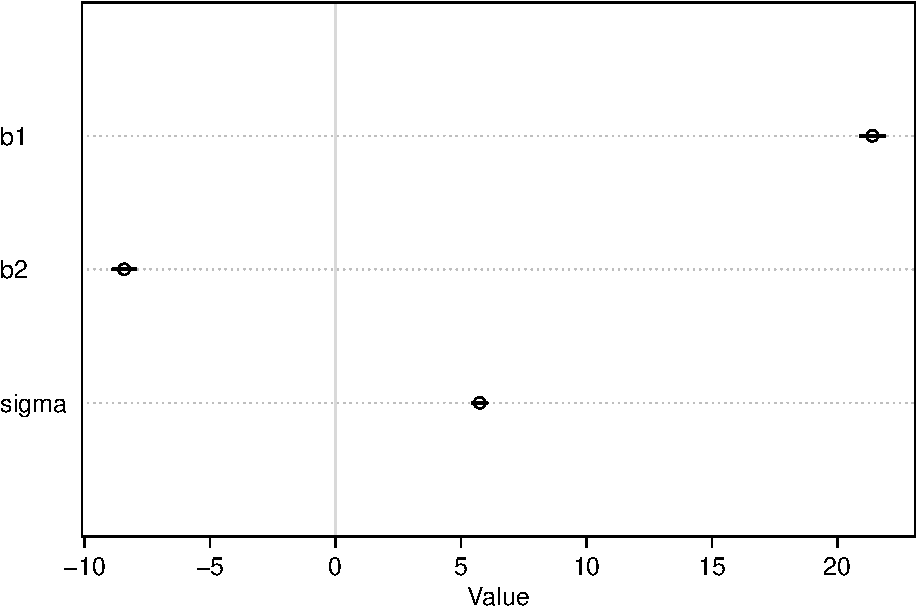
\includegraphics[keepaspectratio]{bookdown-demo_files/figure-latex/unnamed-chunk-59-1.pdf}}

\(\beta_2\) is indeed negative.
In the estimate-plot above I have left out the intercept \(\alpha\) to
make the other coefficients more visible. As you can see, the credible intervals
are very tight. Using prior knowledge an data, the model is very sure about the
coefficients.
We get our \textbf{\href{https://en.wikipedia.org/wiki/Joint_probability_distribution}{joint distribution}}
of the \textbf{four model parameters}.
Let's look at the fit using the mean estimates of the posterior distribution:

\begin{Shaded}
\begin{Highlighting}[]
\CommentTok{\# Summarize the model parameters}
\NormalTok{model\_summary }\OtherTok{\textless{}{-}} \FunctionTok{precis}\NormalTok{(m4}\FloatTok{.1}\NormalTok{)}
\NormalTok{params }\OtherTok{\textless{}{-}} \FunctionTok{as.data.frame}\NormalTok{(model\_summary)}

\CommentTok{\# Extract parameter values}
\NormalTok{a }\OtherTok{\textless{}{-}}\NormalTok{ params[}\StringTok{"a"}\NormalTok{, }\StringTok{"mean"}\NormalTok{]       }\CommentTok{\# Intercept}
\NormalTok{b1 }\OtherTok{\textless{}{-}}\NormalTok{ params[}\StringTok{"b1"}\NormalTok{, }\StringTok{"mean"}\NormalTok{]     }\CommentTok{\# Coefficient for standardized weight}
\NormalTok{b2 }\OtherTok{\textless{}{-}}\NormalTok{ params[}\StringTok{"b2"}\NormalTok{, }\StringTok{"mean"}\NormalTok{]     }\CommentTok{\# Coefficient for squared standardized weight}

\CommentTok{\# Generate a sequence of standardized weights for the fitted curve}
\NormalTok{weight\_seq }\OtherTok{\textless{}{-}} \FunctionTok{seq}\NormalTok{(}\FunctionTok{min}\NormalTok{(d}\SpecialCharTok{$}\NormalTok{weight\_s), }\FunctionTok{max}\NormalTok{(d}\SpecialCharTok{$}\NormalTok{weight\_s), }\AttributeTok{length.out =} \DecValTok{200}\NormalTok{)}

\CommentTok{\# Calculate the fitted values using the quadratic equation}
\NormalTok{height\_fitted }\OtherTok{\textless{}{-}}\NormalTok{ a }\SpecialCharTok{+}\NormalTok{ b1 }\SpecialCharTok{*}\NormalTok{ weight\_seq }\SpecialCharTok{+}\NormalTok{ b2 }\SpecialCharTok{*}\NormalTok{ weight\_seq}\SpecialCharTok{\^{}}\DecValTok{2}

\CommentTok{\# Plot the scatterplot}
\FunctionTok{plot}\NormalTok{(d}\SpecialCharTok{$}\NormalTok{weight\_s, d}\SpecialCharTok{$}\NormalTok{height, }\AttributeTok{pch =} \DecValTok{16}\NormalTok{, }\AttributeTok{col =} \StringTok{"blue"}\NormalTok{,}
     \AttributeTok{xlab =} \StringTok{"Standardized Weight"}\NormalTok{, }\AttributeTok{ylab =} \StringTok{"Height (cm)"}\NormalTok{,}
     \AttributeTok{main =} \StringTok{"Scatterplot with Fitted Curve (Standardized Weight)"}\NormalTok{)}

\CommentTok{\# Add the fitted curve}
\FunctionTok{lines}\NormalTok{(weight\_seq, height\_fitted, }\AttributeTok{col =} \StringTok{"red"}\NormalTok{, }\AttributeTok{lwd =} \DecValTok{2}\NormalTok{)}

\CommentTok{\# Add a legend}
\FunctionTok{legend}\NormalTok{(}\StringTok{"topright"}\NormalTok{, }\AttributeTok{legend =} \FunctionTok{c}\NormalTok{(}\StringTok{"Observed data"}\NormalTok{, }\StringTok{"Fitted curve"}\NormalTok{),}
       \AttributeTok{col =} \FunctionTok{c}\NormalTok{(}\StringTok{"blue"}\NormalTok{, }\StringTok{"red"}\NormalTok{), }\AttributeTok{pch =} \FunctionTok{c}\NormalTok{(}\DecValTok{16}\NormalTok{, }\ConstantTok{NA}\NormalTok{), }\AttributeTok{lty =} \FunctionTok{c}\NormalTok{(}\ConstantTok{NA}\NormalTok{, }\DecValTok{1}\NormalTok{), }\AttributeTok{lwd =} \DecValTok{2}\NormalTok{)}
\end{Highlighting}
\end{Shaded}

\pandocbounded{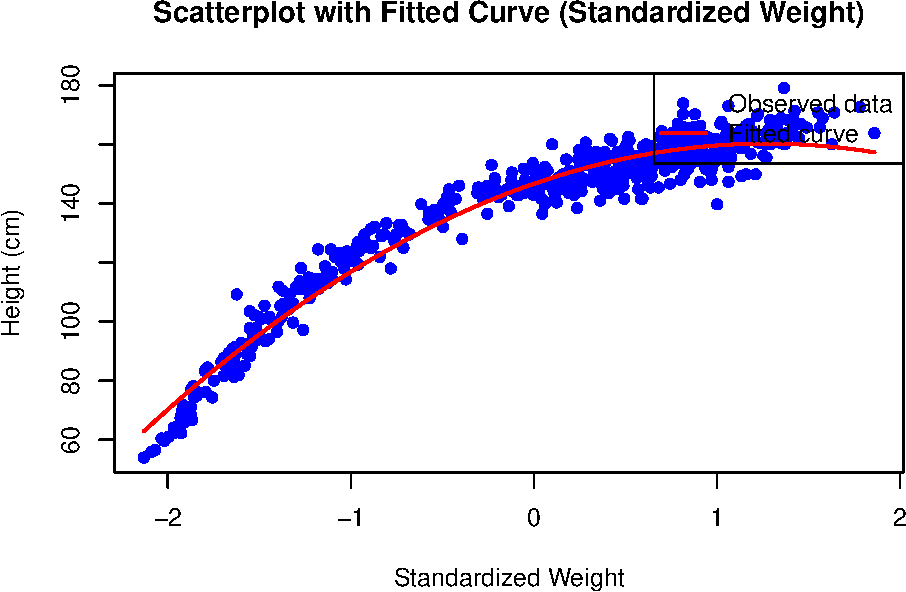
\includegraphics[keepaspectratio]{bookdown-demo_files/figure-latex/unnamed-chunk-60-1.pdf}}

\begin{Shaded}
\begin{Highlighting}[]
       \CommentTok{\# ======== Simulate Heights from Posterior ========}

\CommentTok{\# Prepare new data with the same number of rows as the original data}
\NormalTok{new\_data }\OtherTok{\textless{}{-}} \FunctionTok{data.frame}\NormalTok{(}\AttributeTok{weight\_s =}\NormalTok{ d}\SpecialCharTok{$}\NormalTok{weight\_s, }\AttributeTok{weight\_s2 =}\NormalTok{ d}\SpecialCharTok{$}\NormalTok{weight\_s2)}

\CommentTok{\# Simulate height values from the posterior (same number as original data)}
\NormalTok{sim\_heights }\OtherTok{\textless{}{-}} \FunctionTok{sim}\NormalTok{(m4}\FloatTok{.1}\NormalTok{, }\AttributeTok{data =}\NormalTok{ new\_data, }\AttributeTok{n =} \FunctionTok{nrow}\NormalTok{(d))  }\CommentTok{\# Posterior samples}

\CommentTok{\# Extract random samples from simulated heights}
\NormalTok{height\_samples }\OtherTok{\textless{}{-}} \FunctionTok{apply}\NormalTok{(sim\_heights, }\DecValTok{2}\NormalTok{, }\ControlFlowTok{function}\NormalTok{(x) }\FunctionTok{sample}\NormalTok{(x, }\DecValTok{1}\NormalTok{))}

\CommentTok{\# ======== Plot Observed vs. Simulated Heights ========}

\CommentTok{\# Plot observed data}
\FunctionTok{plot}\NormalTok{(d}\SpecialCharTok{$}\NormalTok{weight\_s, d}\SpecialCharTok{$}\NormalTok{height, }\AttributeTok{pch =} \DecValTok{16}\NormalTok{, }\AttributeTok{col =} \StringTok{"blue"}\NormalTok{,}
     \AttributeTok{xlab =} \StringTok{"Standardized Weight"}\NormalTok{, }\AttributeTok{ylab =} \StringTok{"Height (cm)"}\NormalTok{,}
     \AttributeTok{main =} \StringTok{"Observed vs. Simulated Heights"}\NormalTok{)}

\CommentTok{\# Add simulated height points}
\FunctionTok{points}\NormalTok{(d}\SpecialCharTok{$}\NormalTok{weight\_s, height\_samples, }\AttributeTok{pch =} \DecValTok{16}\NormalTok{, }\AttributeTok{col =} \StringTok{"red"}\NormalTok{)}

\CommentTok{\# Add legend}
\FunctionTok{legend}\NormalTok{(}\StringTok{"topright"}\NormalTok{, }\AttributeTok{legend =} \FunctionTok{c}\NormalTok{(}\StringTok{"Observed Data"}\NormalTok{, }\StringTok{"Simulated Data"}\NormalTok{),}
       \AttributeTok{col =} \FunctionTok{c}\NormalTok{(}\StringTok{"blue"}\NormalTok{, }\StringTok{"red"}\NormalTok{), }\AttributeTok{pch =} \FunctionTok{c}\NormalTok{(}\DecValTok{16}\NormalTok{, }\DecValTok{16}\NormalTok{))}
\end{Highlighting}
\end{Shaded}

\pandocbounded{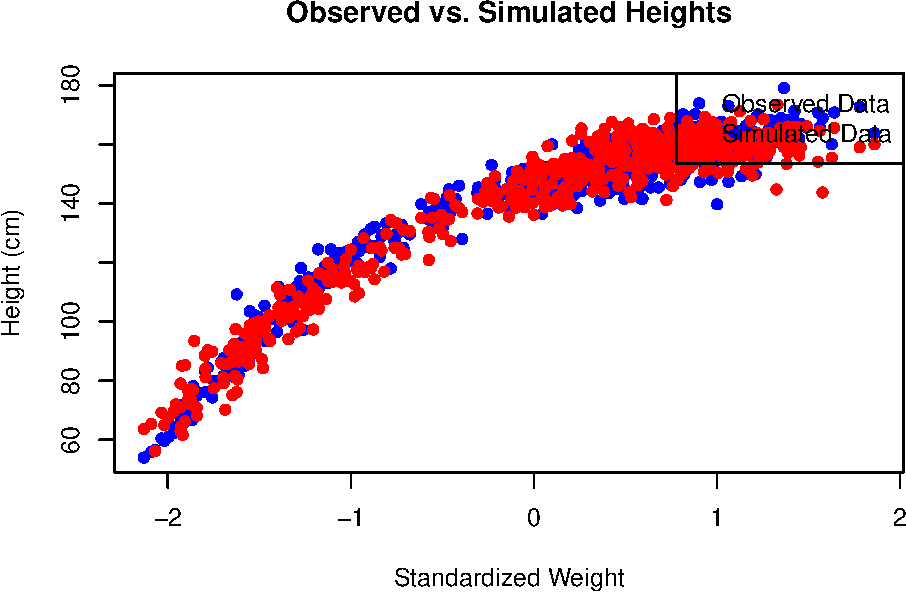
\includegraphics[keepaspectratio]{bookdown-demo_files/figure-latex/unnamed-chunk-60-2.pdf}}

This fits much better than the linear model without the quadratic term. In the book,
there is also a polynomial regression with a cubic term for weight.
The second plot shows the original heights and simulated heights from the
posterior distribution in one plot. This fits quite well.
Maybe this fits even better (see \hyperref[exercise1_multiple_regression]{exercise 1}).

\subsection{Adding another predictor to the model}\label{adding_predictor_bayes}

Since the !Kung San data set has already such a high \(R^2\) with the quadratic term
(and possibly higher with the cubic term), we will use the created data set from
\hyperref[adding_predictor_freq]{below} in the frequentist setting
to estimate the coefficients of the model with two predictors here as well.
We \emph{have} the true but (usually) unknown data generating
mechnisms (for didactic reasons).

We use rather uniformative priors and fit the model using \texttt{quap}:

\begin{Shaded}
\begin{Highlighting}[]
\FunctionTok{library}\NormalTok{(rethinking)}
\FunctionTok{set.seed}\NormalTok{(}\DecValTok{123}\NormalTok{)}
\NormalTok{n }\OtherTok{\textless{}{-}} \DecValTok{100}
\NormalTok{X1 }\OtherTok{\textless{}{-}} \FunctionTok{rnorm}\NormalTok{(n, }\DecValTok{0}\NormalTok{, }\DecValTok{5}\NormalTok{)}
\NormalTok{X2 }\OtherTok{\textless{}{-}} \FunctionTok{rnorm}\NormalTok{(n, }\DecValTok{0}\NormalTok{, }\DecValTok{5}\NormalTok{)}
\NormalTok{Y }\OtherTok{\textless{}{-}} \DecValTok{10} \SpecialCharTok{+} \FloatTok{0.5} \SpecialCharTok{*}\NormalTok{ X1 }\SpecialCharTok{+} \DecValTok{1} \SpecialCharTok{*}\NormalTok{ X2 }\SpecialCharTok{+} \FunctionTok{rnorm}\NormalTok{(n, }\DecValTok{0}\NormalTok{, }\DecValTok{2}\NormalTok{) }\CommentTok{\# true model}
\NormalTok{df }\OtherTok{\textless{}{-}} \FunctionTok{data.frame}\NormalTok{(}\AttributeTok{X1 =}\NormalTok{ X1, }\AttributeTok{X2 =}\NormalTok{ X2, }\AttributeTok{Y =}\NormalTok{ Y)}

\CommentTok{\# fit model}
\NormalTok{m4}\FloatTok{.2} \OtherTok{\textless{}{-}} \FunctionTok{quap}\NormalTok{(}
  \FunctionTok{alist}\NormalTok{(}
\NormalTok{    Y }\SpecialCharTok{\textasciitilde{}} \FunctionTok{dnorm}\NormalTok{(mu, sigma),}
\NormalTok{    mu }\OtherTok{\textless{}{-}}\NormalTok{ a }\SpecialCharTok{+}\NormalTok{ b1}\SpecialCharTok{*}\NormalTok{X1 }\SpecialCharTok{+}\NormalTok{ b2}\SpecialCharTok{*}\NormalTok{X2,}
\NormalTok{    a }\SpecialCharTok{\textasciitilde{}} \FunctionTok{dnorm}\NormalTok{(}\DecValTok{10}\NormalTok{, }\DecValTok{10}\NormalTok{),}
\NormalTok{    b1 }\SpecialCharTok{\textasciitilde{}} \FunctionTok{dnorm}\NormalTok{(}\DecValTok{0}\NormalTok{, }\DecValTok{10}\NormalTok{),}
\NormalTok{    b2 }\SpecialCharTok{\textasciitilde{}} \FunctionTok{dnorm}\NormalTok{(}\DecValTok{0}\NormalTok{, }\DecValTok{10}\NormalTok{),}
\NormalTok{    sigma }\SpecialCharTok{\textasciitilde{}} \FunctionTok{dunif}\NormalTok{(}\DecValTok{0}\NormalTok{, }\DecValTok{50}\NormalTok{)}
\NormalTok{  ), }\AttributeTok{data =}\NormalTok{ df)}
\FunctionTok{precis}\NormalTok{(m4}\FloatTok{.2}\NormalTok{)}
\end{Highlighting}
\end{Shaded}

\begin{verbatim}
##             mean         sd      5.5%      94.5%
## a     10.2700227 0.18934442 9.9674137 10.5726316
## b1     0.4467278 0.04131434 0.3806995  0.5127561
## b2     1.0095082 0.03899992 0.9471788  1.0718377
## sigma  1.8738833 0.13250803 1.6621099  2.0856567
\end{verbatim}

\subsubsection{Checking model assumptions}\label{check_model_bayes}

Andrew Gelman mentions in some of his talks (see \href{https://sites.stat.columbia.edu/gelman/research/published/philosophy_chapter.pdf}{here} for more details)
that many Bayesians he met do not check their models, since they reflect subjective probability.
As I said in the introduction, one should not be afraid to check model predictions against the observed
and probably new data. If a model for predicting BMI performs much worse on a new data set,
we should adapt. We \textbf{do not ask} the question if a model is true or false, but if it is useful or
how badly the model assumptions are violated.

For further, more detailed information on model checking, refer to chapter 6 of
\href{https://sites.stat.columbia.edu/gelman/book/BDA3.pdf}{Gelman's book}.

Anyhow, we plot two posterior predictive checks here.
We test the model within the same data set.
In order to do this, we create new observations
by drawing from the posterior distribution and compare these with the acutally
observed values. This is called \textbf{posterior predictive checks}.

\textbf{First, we plot the observed \(Y\) values against the predicted \(Y\) values (\(=\hat{Y}\))}
from the model (as in Statistical rethinking, Chapter 5).
Although these practically never lie on the line \(y=x\), they should be sufficiently
close to it. We could also compare these two plots with the mean-model (see \hyperref[exercise6_multiple_regression]{exercise 6}).

\begin{Shaded}
\begin{Highlighting}[]
\CommentTok{\# 1) Posterior predictive checks Y vs Y\_hat}
\CommentTok{\# see Statstical Rethinking p 138.}
\CommentTok{\# call link without specifying new data}
\CommentTok{\# so it uses the original data}
\NormalTok{mu }\OtherTok{\textless{}{-}} \FunctionTok{link}\NormalTok{(m4}\FloatTok{.2}\NormalTok{)}

\CommentTok{\# summarize samples accross cases}
\NormalTok{mu\_mean }\OtherTok{\textless{}{-}} \FunctionTok{apply}\NormalTok{(mu, }\DecValTok{2}\NormalTok{, mean)}
\NormalTok{mu\_PI }\OtherTok{\textless{}{-}} \FunctionTok{apply}\NormalTok{(mu, }\DecValTok{2}\NormalTok{, PI, }\AttributeTok{prob =} \FloatTok{0.89}\NormalTok{)}

\CommentTok{\# simulate observations}
\CommentTok{\# again, no new data, so uses original data}
\NormalTok{D\_sim }\OtherTok{\textless{}{-}} \FunctionTok{sim}\NormalTok{(m4}\FloatTok{.2}\NormalTok{, }\AttributeTok{n =} \FloatTok{1e4}\NormalTok{)}
\NormalTok{D\_PI }\OtherTok{\textless{}{-}} \FunctionTok{apply}\NormalTok{(D\_sim, }\DecValTok{2}\NormalTok{, PI, }\AttributeTok{prob =} \FloatTok{0.89}\NormalTok{)}

\FunctionTok{plot}\NormalTok{(mu\_mean }\SpecialCharTok{\textasciitilde{}}\NormalTok{ df}\SpecialCharTok{$}\NormalTok{Y, }\AttributeTok{col =}\NormalTok{ rangi2, }\AttributeTok{ylim =} \FunctionTok{range}\NormalTok{(mu\_PI), }
     \AttributeTok{xlab =} \StringTok{"Observed Y"}\NormalTok{, }\AttributeTok{ylab =} \StringTok{"Model{-}Predicted Y"}\NormalTok{)}
\FunctionTok{abline}\NormalTok{(}\AttributeTok{a =} \DecValTok{0}\NormalTok{, }\AttributeTok{b =} \DecValTok{1}\NormalTok{, }\AttributeTok{lty =} \DecValTok{2}\NormalTok{)}
\ControlFlowTok{for}\NormalTok{(i }\ControlFlowTok{in} \DecValTok{1}\SpecialCharTok{:}\FunctionTok{nrow}\NormalTok{(df)) }\FunctionTok{lines}\NormalTok{(}\FunctionTok{rep}\NormalTok{(df}\SpecialCharTok{$}\NormalTok{Y[i], }\DecValTok{2}\NormalTok{), mu\_PI[,i], }\AttributeTok{col =}\NormalTok{ rangi2)}
\end{Highlighting}
\end{Shaded}

\pandocbounded{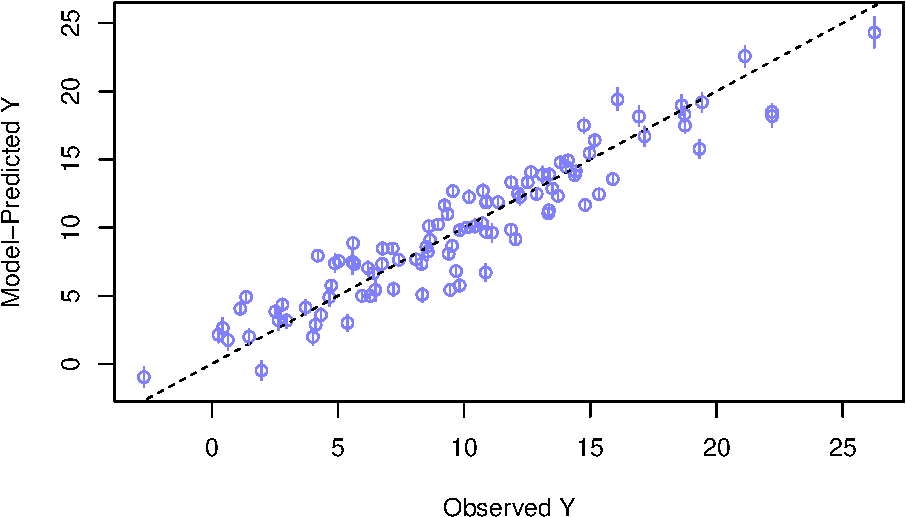
\includegraphics[keepaspectratio]{bookdown-demo_files/figure-latex/unnamed-chunk-62-1.pdf}}

As we can see, the model fits the data quite well. The points are close to the dashed line (\(y=x\)).
No under- or overestimation is visible. The model seems to capture the relationship between the predictors \(X_1\) and \(X_2\)
and the dependent variable \(Y\) quite well - at least in a predictive sense. If there were patches of data points above or below the dashed line,
we would probably have to reconsider the model definition and think about why these points are not captured by the model.

\textbf{Next, we plot the posterior predictive plots} analog to the upper left in the \texttt{check\_model} output.

\begin{Shaded}
\begin{Highlighting}[]
\FunctionTok{library}\NormalTok{(scales)  }\CommentTok{\# For the alpha function to adjust transparency}
\end{Highlighting}
\end{Shaded}

\begin{verbatim}
## 
## Attaching package: 'scales'
\end{verbatim}

\begin{verbatim}
## The following object is masked from 'package:purrr':
## 
##     discard
\end{verbatim}

\begin{verbatim}
## The following object is masked from 'package:readr':
## 
##     col_factor
\end{verbatim}

\begin{Shaded}
\begin{Highlighting}[]
\CommentTok{\# 2) Posterior predictive densities}
\CommentTok{\# Simulate observations using the posterior predictive distribution}
\NormalTok{D\_sim }\OtherTok{\textless{}{-}} \FunctionTok{sim}\NormalTok{(m4}\FloatTok{.2}\NormalTok{, }\AttributeTok{n =} \FloatTok{1e4}\NormalTok{)  }\CommentTok{\# Generate 10,000 simulated datasets}

\CommentTok{\# Calculate densities for all samples}
\NormalTok{densities }\OtherTok{\textless{}{-}} \FunctionTok{apply}\NormalTok{(D\_sim, }\DecValTok{1}\NormalTok{, density)}

\CommentTok{\# Find the maximum density value for setting the y{-}axis limits}
\NormalTok{max\_density }\OtherTok{\textless{}{-}} \FunctionTok{max}\NormalTok{(}\FunctionTok{sapply}\NormalTok{(densities, }\ControlFlowTok{function}\NormalTok{(d) }\FunctionTok{max}\NormalTok{(d}\SpecialCharTok{$}\NormalTok{y)))}

\CommentTok{\# Create the density plot with predefined ylim}
\FunctionTok{plot}\NormalTok{(}\ConstantTok{NULL}\NormalTok{, }\AttributeTok{xlim =} \FunctionTok{range}\NormalTok{(df}\SpecialCharTok{$}\NormalTok{Y), }\AttributeTok{ylim =} \FunctionTok{c}\NormalTok{(}\DecValTok{0}\NormalTok{, max\_density),}
     \AttributeTok{xlab =} \StringTok{"Y"}\NormalTok{, }\AttributeTok{ylab =} \StringTok{"Density"}\NormalTok{,}
     \AttributeTok{main =} \StringTok{"Comparison of Observed and Predicted Densities"}\NormalTok{)}

\CommentTok{\# Add 100 posterior predictive density lines}
\FunctionTok{set.seed}\NormalTok{(}\DecValTok{42}\NormalTok{)  }\CommentTok{\# For reproducibility}
\NormalTok{n\_lines }\OtherTok{\textless{}{-}} \DecValTok{100}
\NormalTok{samples }\OtherTok{\textless{}{-}} \FunctionTok{sample}\NormalTok{(}\DecValTok{1}\SpecialCharTok{:}\FloatTok{1e4}\NormalTok{, n\_lines)  }\CommentTok{\# Randomly sample 100 posterior predictive datasets}
\ControlFlowTok{for}\NormalTok{ (s }\ControlFlowTok{in}\NormalTok{ samples) \{}
  \FunctionTok{lines}\NormalTok{(}\FunctionTok{density}\NormalTok{(D\_sim[s, ]), }\AttributeTok{col =} \FunctionTok{alpha}\NormalTok{(}\StringTok{"lightblue"}\NormalTok{, }\FloatTok{0.3}\NormalTok{), }\AttributeTok{lwd =} \DecValTok{1}\NormalTok{)}
\NormalTok{\}}

\CommentTok{\# Add the density line for the observed Y values}
\NormalTok{obs\_density }\OtherTok{\textless{}{-}} \FunctionTok{density}\NormalTok{(df}\SpecialCharTok{$}\NormalTok{Y)}
\FunctionTok{lines}\NormalTok{(obs\_density}\SpecialCharTok{$}\NormalTok{x, obs\_density}\SpecialCharTok{$}\NormalTok{y, }\AttributeTok{col =} \StringTok{"green"}\NormalTok{, }\AttributeTok{lwd =} \DecValTok{2}\NormalTok{)}

\CommentTok{\# Add legend}
\FunctionTok{legend}\NormalTok{(}\StringTok{"topright"}\NormalTok{, }\AttributeTok{legend =} \FunctionTok{c}\NormalTok{(}\StringTok{"Posterior Predictive Densities"}\NormalTok{, }\StringTok{"Observed Density"}\NormalTok{),}
       \AttributeTok{col =} \FunctionTok{c}\NormalTok{(}\StringTok{"lightblue"}\NormalTok{, }\StringTok{"green"}\NormalTok{), }\AttributeTok{lty =} \DecValTok{1}\NormalTok{, }\AttributeTok{lwd =} \FunctionTok{c}\NormalTok{(}\DecValTok{1}\NormalTok{, }\DecValTok{2}\NormalTok{))}
\end{Highlighting}
\end{Shaded}

\pandocbounded{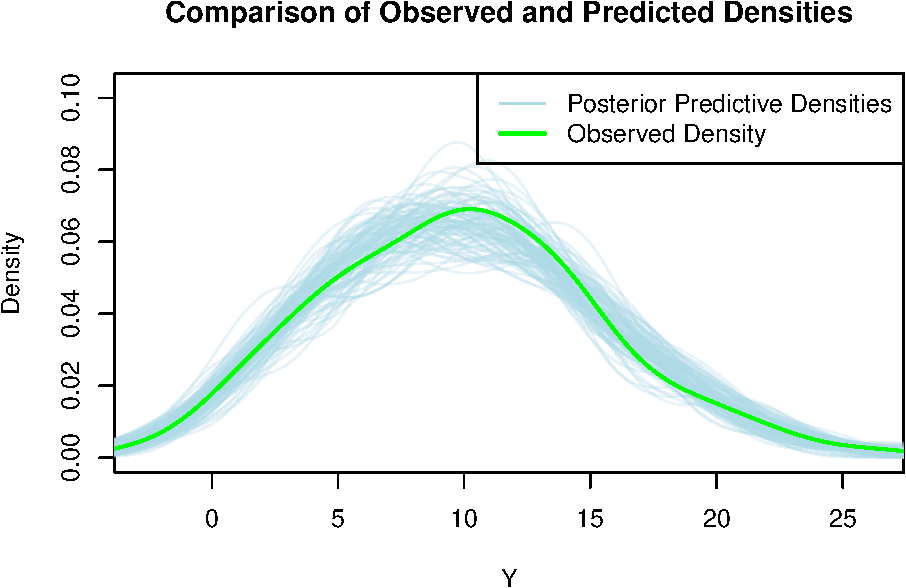
\includegraphics[keepaspectratio]{bookdown-demo_files/figure-latex/unnamed-chunk-63-1.pdf}}

The light blue lines show distributions of model predicted \(Y\) values.
The green line shows the distribution of the observed \(Y\) values.
As we can see, there seem to be no systematic differences between the observed and predicted values.
The model seems to capture the relationship well.
If we see systematic deviations here, we need to reconsider the model definition.

\textbf{Example}: If you want to predict pain (\(Y\) variable) and you have a lot of zeros (pain-free participants)
you will probably see a discrepancy between the observed and predicted values in this plot.
What could you do? You could use a two step process (model the probability that a person is pain-free
and then model the pain intensity for the people who have pain) or use a different model (like a zero-inflated model).

Note that we did not explicitely assume normally distributed errors in the model definition above,
so we won't check this here but in the Frequentist framework below.

\section{Linear regression with 2 predictors in the Frequentist Framework}\label{linear-regression-with-2-predictors-in-the-frequentist-framework}

To reiterate from the last chapter:
In full, the \textbf{classical linear regression model} can be written as
(see p.~21-22 in Westfall):

\[ Y_i|X_i = x_i \sim_{independent} N(\beta_0 + \beta_1 x_{i1} + \dots \beta_k x_{ik},\sigma^2)\]
for \(i = 1, \dots, n\).

The \(Y_i\) are independently normally distributed \emph{conditioned} on the predictors
having the values \(X_i = x_i\). Each conditional distribution has an expected value (\(\mu\))
that is a linear function of the predictors and a constant variance \(\sigma^2\).

If the assumptions of the classical linear regression model are met, the least squares
estimators (OLS) are the best (smallest variance) linear unbiased (on average correct) estimators
- so-called: \textbf{BLUE} - of the parameters.

\subsection{Adding a transformed predictor to the model}\label{adding_transformed_predictor_freq}

No, let's fit the same model as \hyperref[adding_transformed_predictor_bayes]{above} in the Bayesian framework.

The model is:

\[height_i = \alpha + \beta_1 weight_i + \beta_2 weight_i^2 + \varepsilon_i\]
whereas
\[\varepsilon_i \sim N(0, \sigma)\]

And if you build the expectation on both sides for fixed \(weight_i\), you get:

\[\mathbb{E}(height_i|weight_i) = \alpha + \beta_1 weight_i + \beta_2 weight_i^2\]

The last line means, the expected height of a person given a certain weight depends
quadratically on the weight. The error term \(\varepsilon_i\) is on average zero, hence it goes away here.
Remember the \href{https://en.wikipedia.org/wiki/Law_of_large_numbers\#Weak_law}{law of large numbers}:
The sample mean \(\bar{\varepsilon_i}\) approaches the expected value \(\mathbb{E}(\varepsilon_i)=0\)
as the sample size increases. If you drew many samples (from the true model)
and average over the error terms, the average will approach zero.
Think of \href{https://github.com/jdegenfellner/ZHAW_Teaching/blob/main/Wiggle_in_simple_linear_regression.R}{this} animated
graph if you need a dynamic image of the regression model.
The weights are considered fixed and therefore do not change when building the expectation.

We are looking for fixed, but unknown, parameters \(\alpha\), \(\beta_1\), \(\beta_2\) and \(\sigma\).
The fixed \(\sigma\) indicates that the observations \emph{wiggle} around the expected value
equally strong not matter which weight we have. This is called \textbf{homoscedasticity}.

Let's fit the model using the \texttt{lm} function in R which uses
\href{https://en.wikipedia.org/wiki/Least_squares}{least squares} to estimate the parameters.
At this point I could torture you with \href{https://en.wikipedia.org/wiki/Matrix_(mathematics)}{matrix algebra}
and show you the \href{https://en.wikipedia.org/wiki/Linear_least_squares}{normal equations} for linear regression,
but I will spare you for now.
Note that the least squares algorithm for fitting the curve works for all
kinds of functional forms. For example, we could also fit an exponential curve using the same
technique (see \hyperref[exercise9_multiple_regression]{exercise 9}).

\begin{Shaded}
\begin{Highlighting}[]
\CommentTok{\# scale weight}
\NormalTok{d}\SpecialCharTok{$}\NormalTok{weight\_s }\OtherTok{\textless{}{-}} \FunctionTok{scale}\NormalTok{(d}\SpecialCharTok{$}\NormalTok{weight)}
\CommentTok{\# Fit the model}
\NormalTok{m4}\FloatTok{.2} \OtherTok{\textless{}{-}} \FunctionTok{lm}\NormalTok{(height }\SpecialCharTok{\textasciitilde{}}\NormalTok{ weight\_s }\SpecialCharTok{+} \FunctionTok{I}\NormalTok{(weight\_s}\SpecialCharTok{\^{}}\DecValTok{2}\NormalTok{), }\AttributeTok{data =}\NormalTok{ d)}
\FunctionTok{summary}\NormalTok{(m4}\FloatTok{.2}\NormalTok{)}
\end{Highlighting}
\end{Shaded}

\begin{verbatim}
## 
## Call:
## lm(formula = height ~ weight_s + I(weight_s^2), data = d)
## 
## Residuals:
##      Min       1Q   Median       3Q      Max 
## -19.9689  -3.9794   0.2364   3.9262  19.5182 
## 
## Coefficients:
##               Estimate Std. Error t value Pr(>|t|)    
## (Intercept)   146.6604     0.3748  391.30   <2e-16 ***
## weight_s       21.4149     0.2908   73.64   <2e-16 ***
## I(weight_s^2)  -8.4123     0.2822  -29.80   <2e-16 ***
## ---
## Signif. codes:  0 '***' 0.001 '**' 0.01 '*' 0.05 '.' 0.1 ' ' 1
## 
## Residual standard error: 5.766 on 541 degrees of freedom
## Multiple R-squared:  0.9565, Adjusted R-squared:  0.9564 
## F-statistic:  5952 on 2 and 541 DF,  p-value: < 2.2e-16
\end{verbatim}

\begin{Shaded}
\begin{Highlighting}[]
\FunctionTok{mean}\NormalTok{(d}\SpecialCharTok{$}\NormalTok{height)}
\end{Highlighting}
\end{Shaded}

\begin{verbatim}
## [1] 138.2636
\end{verbatim}

\begin{Shaded}
\begin{Highlighting}[]
\FunctionTok{confint}\NormalTok{(m4}\FloatTok{.2}\NormalTok{, }\AttributeTok{level =} \FloatTok{0.94}\NormalTok{)}
\end{Highlighting}
\end{Shaded}

\begin{verbatim}
##                      3 %       97 %
## (Intercept)   145.954018 147.366836
## weight_s       20.866788  21.962979
## I(weight_s^2)  -8.944251  -7.880337
\end{verbatim}

See \texttt{?I} in R. This command is used so that R knows that it should
treat the ``\^{}2'' as ``square'' and not as formula syntax.
We could also create a new variable as before. Whatever you prefer.

\subsubsection{Interpretation of output and coefficients}\label{interpretation_output_freq_quadratic}

\begin{itemize}
\tightlist
\item
  The intercept \(\alpha\) is the \textbf{model-predicted height} of a person of \textbf{average weight}
  (\(weight_s=0\) for a person of average weight).
  Note that this is not equal to the average height (\(138.2636~cm\)) of the people in the data set
  (see \hyperref[exercise12_multiple_regression]{exercise 12}).
\item
  The residuals have range from \(-19.97\) to \(19.51\). So, the model maximally
  overestimates the heights by \(19.97\) cm and underestimates by \(19.51\) cm.
  These numbers are plausible when you look at the scatterplot with the fitted
  curve.
\item
  The coefficients \(\beta_1\) and \(\beta_2\) agree with the Bayes estimates.
  Specifically, \(\beta_2\) is non-zero indicating curvature. You cannot directly interpret the coefficients
  as in the non-quadratic case since, for instance, you cannot change \(weight^2\) by one unit
  and hold \(weight\) constant at the same time. Refer to Peter Westfall's book section 9.1. for all the details.
\item
  If you like \(p\)-values: All the hypotheses that the coefficients are zero
  are rejected. The \(p\)-values are very small. The values of the test statistics can not be explained
  by chance alone. On the other hand, for at least \(\beta_1\) and
  and the global test this is not a surprise when you look at the scatterplot.
  After having fit many models, you would have guessed that all three parameters
  are solidly non-zero. The intercept is not zero since a person of average weight probably
  has non-zero height. \(\beta_1\) is non-zero since you can easily imagine a linear
  trend line with positive slope going through the data, and \(\beta_2\) is non-zero
  since there is clearly (non-trivial) curvature in the scatterplot.
\item
  The \(R^2\) is a whopping \(0.96\) which could be a sign of overfitting, but
  in this case we conclude that the true relationship is caputured rather well.
  \href{https://en.wikipedia.org/wiki/Overfitting}{Overfitting} would occur if
  our curve would rather fit the noise in the data than
  the underying trend.
\end{itemize}

\subsubsection{Checking model assumptions}\label{checking-model-assumptions}

\begin{Shaded}
\begin{Highlighting}[]
\FunctionTok{check\_model}\NormalTok{(m4}\FloatTok{.2}\NormalTok{)}
\end{Highlighting}
\end{Shaded}

\begin{verbatim}
## Some of the variables were in matrix-format - probably you used
##   `scale()` on your data?
##   If so, and you get an error, please try `datawizard::standardize()` to
##   standardize your data.
## Some of the variables were in matrix-format - probably you used
##   `scale()` on your data?
##   If so, and you get an error, please try `datawizard::standardize()` to
##   standardize your data.
\end{verbatim}

\pandocbounded{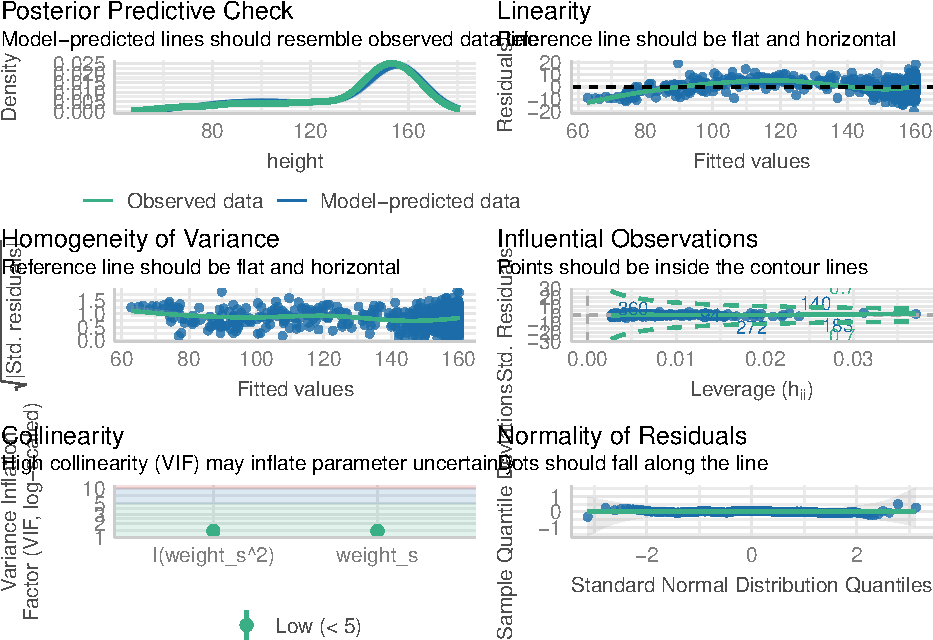
\includegraphics[keepaspectratio]{bookdown-demo_files/figure-latex/unnamed-chunk-65-1.pdf}}

If we want to be perfectionists, we could remark that (upper right plot)
in the lower fitted values the residuals are more negative,
meaning that the model overestimates the heights in this region.
In the middle region the model underestimates a bit and we can see
a positive tendency in the residuals. Apart from that,
the diagnostic plots look excellent.

\subsection{Adding another predictor to the model}\label{adding_predictor_freq}

Now, we add another predictor to the model. We use \(X_1\) and \(X_2\)
\textbf{simultaneously} to predict \(Y\). We are now in the lucky situation that
we can still visualize the situation in 3D. The regression line from simple
linear regression
becomes a \href{https://stackoverflow.com/questions/47344850/scatterplot3d-regression-plane-with-residuals}{plane}.
The vertical distances between the data points and the plane are the residuals.
See \href{https://rpubs.com/pjozefek/576206}{here} or
\href{https://www.sthda.com/english/wiki/scatterplot3d-3d-graphics-r-software-and-data-visualization}{here}
at the end for examples.
Minimizing the sum of the squared errors gives again
the estimates for the coefficients.

For demonstration purposes, we can \textbf{create data ourselves} with known
coefficients. This is the same as \hyperref[adding_predictor_bayes]{above}.
This is the true model, which we usually do not know:

\[ Y_i = \beta_0 + \beta_1 X_{1i} + \beta_2 X_{2i} + \varepsilon_i\]
\[ \varepsilon_i \sim N(0, \sigma^2)\]
\[ \mathbb{E}(Y_i|X_1 = x_1; X_2 = x_2) = \beta_0 + \beta_1 x_1 + \beta_2 x_2\]
\[ i = 1 \ldots n\]

for example:

\[ Y_i = 10 + 0.5 \cdot X_{1i} + 1 \cdot X_{2i} + \varepsilon_i\]
\[ \varepsilon_i \sim N(0, 5)\]
\[ \mathbb{E}(Y_i|X_1 = x_1; X_2 = x_2) = 10 + 0.5 x_1 + 1 x_2\]
\[ i = 1 \ldots n\]

According to the model, the conditional expected value of \(Y_i\) given \(X_1 = x_1\) and \(X_2 = x_2\)
is a linear function of \(x_1\) and \(x_2\). Note, that small letters are realized values
of random variables. Also note, that in the expectation the error term goes away, since
\(\mathbb{E}(\varepsilon_i) = 0\).

\begin{itemize}
\tightlist
\item
  If \(X_1\) increases by one unit, \(Y\) increases by \(0.5\) units on average (in expectation).
\item
  If \(X_2\) increases by one unit, \(Y\) increases by \(1\) unit on average (in expectation).
\item
  If \(X_1\) and \(X_2\) are zero, \(Y\) is \(10\) on average (in expectation).
\end{itemize}

Why in expectation? Because there is still the error term which makes the whole thing random!
We can see that an increase in \(X_1\) does not influence the relationship between \(X_2\) and \(Y\).
Hence, there is \textbf{no interaction} between \(X_1\) and \(X_2\) with respect to \(Y\).

Now lets's draw 100 points from this model, fit the model and add the plane:

\begin{Shaded}
\begin{Highlighting}[]
\FunctionTok{library}\NormalTok{(plotly)}

\FunctionTok{set.seed}\NormalTok{(}\DecValTok{123}\NormalTok{)}
\NormalTok{n }\OtherTok{\textless{}{-}} \DecValTok{100}
\NormalTok{X1 }\OtherTok{\textless{}{-}} \FunctionTok{rnorm}\NormalTok{(n, }\DecValTok{0}\NormalTok{, }\DecValTok{5}\NormalTok{)}
\NormalTok{X2 }\OtherTok{\textless{}{-}} \FunctionTok{rnorm}\NormalTok{(n, }\DecValTok{0}\NormalTok{, }\DecValTok{5}\NormalTok{)}
\NormalTok{Y }\OtherTok{\textless{}{-}} \DecValTok{10} \SpecialCharTok{+} \FloatTok{0.5} \SpecialCharTok{*}\NormalTok{ X1 }\SpecialCharTok{+} \DecValTok{1} \SpecialCharTok{*}\NormalTok{ X2 }\SpecialCharTok{+} \FunctionTok{rnorm}\NormalTok{(n, }\DecValTok{0}\NormalTok{, }\DecValTok{2}\NormalTok{)}
\NormalTok{d }\OtherTok{\textless{}{-}} \FunctionTok{data.frame}\NormalTok{(}\AttributeTok{X1 =}\NormalTok{ X1, }\AttributeTok{X2 =}\NormalTok{ X2, }\AttributeTok{Y =}\NormalTok{ Y)}

\CommentTok{\# Fit the model}
\NormalTok{m4}\FloatTok{.3} \OtherTok{\textless{}{-}} \FunctionTok{lm}\NormalTok{(Y }\SpecialCharTok{\textasciitilde{}}\NormalTok{ X1 }\SpecialCharTok{+}\NormalTok{ X2, }\AttributeTok{data =}\NormalTok{ d)}
\FunctionTok{summary}\NormalTok{(m4}\FloatTok{.3}\NormalTok{)}
\end{Highlighting}
\end{Shaded}

\begin{verbatim}
## 
## Call:
## lm(formula = Y ~ X1 + X2, data = d)
## 
## Residuals:
##     Min      1Q  Median      3Q     Max 
## -3.7460 -1.3215 -0.2489  1.2427  4.1597 
## 
## Coefficients:
##             Estimate Std. Error t value Pr(>|t|)    
## (Intercept) 10.27013    0.19228   53.41   <2e-16 ***
## X1           0.44673    0.04195   10.65   <2e-16 ***
## X2           1.00952    0.03960   25.49   <2e-16 ***
## ---
## Signif. codes:  0 '***' 0.001 '**' 0.01 '*' 0.05 '.' 0.1 ' ' 1
## 
## Residual standard error: 1.903 on 97 degrees of freedom
## Multiple R-squared:  0.8839, Adjusted R-squared:  0.8815 
## F-statistic: 369.1 on 2 and 97 DF,  p-value: < 2.2e-16
\end{verbatim}

\begin{Shaded}
\begin{Highlighting}[]
\CommentTok{\# Create a grid for the plane}
\NormalTok{X1\_grid }\OtherTok{\textless{}{-}} \FunctionTok{seq}\NormalTok{(}\FunctionTok{min}\NormalTok{(d}\SpecialCharTok{$}\NormalTok{X1), }\FunctionTok{max}\NormalTok{(d}\SpecialCharTok{$}\NormalTok{X1), }\AttributeTok{length.out =} \DecValTok{20}\NormalTok{)}
\NormalTok{X2\_grid }\OtherTok{\textless{}{-}} \FunctionTok{seq}\NormalTok{(}\FunctionTok{min}\NormalTok{(d}\SpecialCharTok{$}\NormalTok{X2), }\FunctionTok{max}\NormalTok{(d}\SpecialCharTok{$}\NormalTok{X2), }\AttributeTok{length.out =} \DecValTok{20}\NormalTok{)}
\NormalTok{grid }\OtherTok{\textless{}{-}} \FunctionTok{expand.grid}\NormalTok{(}\AttributeTok{X1 =}\NormalTok{ X1\_grid, }\AttributeTok{X2 =}\NormalTok{ X2\_grid)}

\CommentTok{\# Predict the values for the grid}
\NormalTok{grid}\SpecialCharTok{$}\NormalTok{Y }\OtherTok{\textless{}{-}} \FunctionTok{predict}\NormalTok{(m4}\FloatTok{.3}\NormalTok{, }\AttributeTok{newdata =}\NormalTok{ grid)}

\CommentTok{\# Convert the grid into a matrix for the plane}
\NormalTok{plane\_matrix }\OtherTok{\textless{}{-}} \FunctionTok{matrix}\NormalTok{(grid}\SpecialCharTok{$}\NormalTok{Y, }\AttributeTok{nrow =} \FunctionTok{length}\NormalTok{(X1\_grid), }\AttributeTok{ncol =} \FunctionTok{length}\NormalTok{(X2\_grid))}

\CommentTok{\# Create the interactive 3D plot}
\FunctionTok{plot\_ly}\NormalTok{() }\SpecialCharTok{\%\textgreater{}\%}
  \FunctionTok{add\_markers}\NormalTok{(}
    \AttributeTok{x =}\NormalTok{ d}\SpecialCharTok{$}\NormalTok{X2, }\AttributeTok{y =}\NormalTok{ d}\SpecialCharTok{$}\NormalTok{X1, }\AttributeTok{z =}\NormalTok{ d}\SpecialCharTok{$}\NormalTok{Y,}
    \AttributeTok{marker =} \FunctionTok{list}\NormalTok{(}\AttributeTok{color =} \StringTok{"blue"}\NormalTok{, }\AttributeTok{size =} \DecValTok{5}\NormalTok{),}
    \AttributeTok{name =} \StringTok{"Data Points"}
\NormalTok{  ) }\SpecialCharTok{\%\textgreater{}\%}
  \FunctionTok{add\_surface}\NormalTok{(}
    \AttributeTok{x =}\NormalTok{ X1\_grid, }\AttributeTok{y =}\NormalTok{ X2\_grid, }\AttributeTok{z =}\NormalTok{ plane\_matrix,}
    \AttributeTok{colorscale =} \FunctionTok{list}\NormalTok{(}\FunctionTok{c}\NormalTok{(}\DecValTok{0}\NormalTok{, }\DecValTok{1}\NormalTok{), }\FunctionTok{c}\NormalTok{(}\StringTok{"red"}\NormalTok{, }\StringTok{"pink"}\NormalTok{)),}
    \AttributeTok{showscale =} \ConstantTok{FALSE}\NormalTok{,}
    \AttributeTok{opacity =} \FloatTok{0.7}\NormalTok{,}
    \AttributeTok{name =} \StringTok{"Fitted Plane"}
\NormalTok{  ) }\SpecialCharTok{\%\textgreater{}\%}
\NormalTok{  plotly}\SpecialCharTok{::}\FunctionTok{layout}\NormalTok{(}
    \AttributeTok{scene =} \FunctionTok{list}\NormalTok{(}
      \AttributeTok{xaxis =} \FunctionTok{list}\NormalTok{(}\AttributeTok{title =} \StringTok{"X1"}\NormalTok{),}
      \AttributeTok{yaxis =} \FunctionTok{list}\NormalTok{(}\AttributeTok{title =} \StringTok{"X2"}\NormalTok{),}
      \AttributeTok{zaxis =} \FunctionTok{list}\NormalTok{(}\AttributeTok{title =} \StringTok{"Y"}\NormalTok{)}
\NormalTok{    ),}
    \AttributeTok{title =} \StringTok{"Interactive 3D Scatterplot with Fitted Plane"}
\NormalTok{  )}
\end{Highlighting}
\end{Shaded}

\begin{verbatim}
## file:////private/var/folders/pm/jd6n6gj10371_bml1gh8sc5w0000gn/T/RtmpOZ9C46/file5f901b49a069/widget5f907ec25b7d.html screenshot completed
\end{verbatim}

\pandocbounded{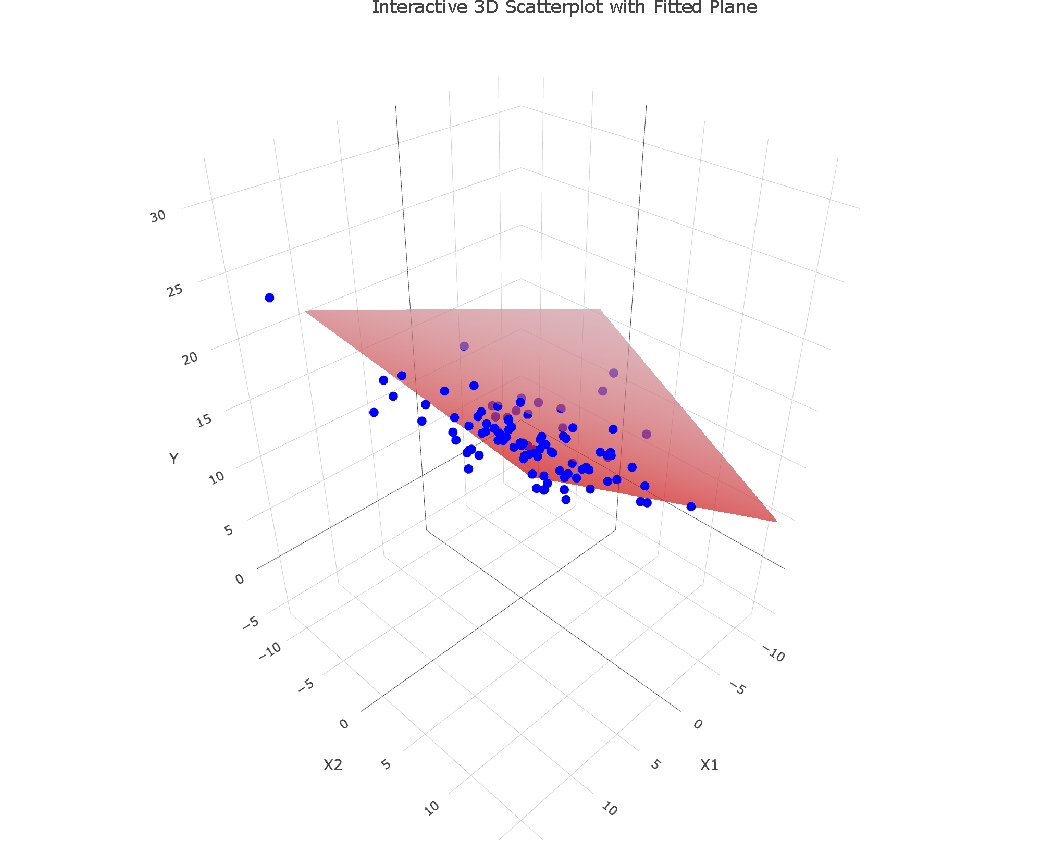
\includegraphics[keepaspectratio]{bookdown-demo_files/figure-latex/unnamed-chunk-66-1.pdf}}

This is, of course, a very idealized situation. There is no curvature in the plane,
no interaction, no outliers, no heteroscadasticity. It's the simplest case of multiple regression
with 2 predictors. Reality is - usually - more complicated.

Let's look at the summary output and check model assumptions:

\begin{Shaded}
\begin{Highlighting}[]
\FunctionTok{summary}\NormalTok{(m4}\FloatTok{.3}\NormalTok{)}
\end{Highlighting}
\end{Shaded}

\begin{verbatim}
## 
## Call:
## lm(formula = Y ~ X1 + X2, data = d)
## 
## Residuals:
##     Min      1Q  Median      3Q     Max 
## -3.7460 -1.3215 -0.2489  1.2427  4.1597 
## 
## Coefficients:
##             Estimate Std. Error t value Pr(>|t|)    
## (Intercept) 10.27013    0.19228   53.41   <2e-16 ***
## X1           0.44673    0.04195   10.65   <2e-16 ***
## X2           1.00952    0.03960   25.49   <2e-16 ***
## ---
## Signif. codes:  0 '***' 0.001 '**' 0.01 '*' 0.05 '.' 0.1 ' ' 1
## 
## Residual standard error: 1.903 on 97 degrees of freedom
## Multiple R-squared:  0.8839, Adjusted R-squared:  0.8815 
## F-statistic: 369.1 on 2 and 97 DF,  p-value: < 2.2e-16
\end{verbatim}

\begin{Shaded}
\begin{Highlighting}[]
\FunctionTok{check\_model}\NormalTok{(m4}\FloatTok{.3}\NormalTok{)}
\end{Highlighting}
\end{Shaded}

\pandocbounded{\includegraphics[keepaspectratio]{bookdown-demo_files/figure-latex/unnamed-chunk-67-1.pdf}}

We could repeat this simulation to get a feeling for the variability.
The posterior predictive checks look nice. In this case, we \emph{know} that the model is true.

\subsubsection{Adding variables to the model and why}\label{adding-variables-to-the-model-and-why}

This is a very complex question. We will go into it in later chapters and the next course (Methodenvertiefung).
At this point we can say this:
We add variables to the model (and probably use
other models apart from linear regression) \emph{depending} on the goal at hand (prediction or explanation).
Prediction seems to be easier than explanation. For instance, within linear models and
just a handful of predictors, one can even brute force the problem by searching through
all subsets of predictors. If that is not possible, one could use clever algortithms, like
\href{https://www.sthda.com/english/articles/37-model-selection-essentials-in-r/155-best-subsets-regression-essentials-in-r/}{best subest selection}.

\begin{itemize}
\tightlist
\item
  What is \textbf{not} a good idea is to throw all variables into the model and hope for the best -
  especially if we want to learn the true relationships between the variables.
\item
  What is also not a good idea is to select variables depending on the \(p\)-values of the coefficients (Westfall Chapter 11).
\item
  \textbf{Leaving variables out}, that are important, can lead to biased estimates of the coefficients
  (\href{https://en.wikipedia.org/wiki/Omitted-variable_bias}{omitted variable bias}).
\item
  Importantly, also \textbf{adding variables} can hurt conclusions from the model (see Statistical Rethinking 6.2).
\end{itemize}

\subsection{\texorpdfstring{Interaction Term \(X_1 \times X_2\)}{Interaction Term X\_1 \textbackslash times X\_2}}\label{interaction_term}

I recommend reading the excellent explanations about interactions
in John Kruschke's book \href{https://nyu-cdsc.github.io/learningr/assets/kruschke_bayesian_in_R.pdf}{Doing Bayesian Data Analysis},
15.2.2 und 15.2.3. Peter Westfall also has a nice explanation in his \href{https://www.routledge.com/Understanding-Regression-Analysis-A-Conditional-Distribution-Approach/Westfall-Arias/p/book/9780367493516?srsltid=AfmBOore3O_Ciecl0TTkr9AjPIY1d6OmbQa7o7IAdKpTSkD8s9HkwzD4}{book}
in section 9.3.

Our statistical model is now:

\[ Y_i = \beta_0 + \beta_1 X_{1i} + \beta_2 X_{2i} + \mathbf{\beta_3 X_{1i} \times X_{2i}} + \varepsilon_i\]
\[ \varepsilon_i \sim N(0, \sigma^2)\]
\[ \mathbb{E}(Y_i|X_1 = x_1; X_2 = x_2) = \beta_0 + \beta_1 x_{1} + \beta_2 x_{2} + \beta_3 x_{1} \times x_{2}\]
\[ i = 1 \ldots n\]

for example:

\[ Y_i = 10 + 0.5 \cdot X_{1i} + 1 \cdot X_{2i} + 0.89 \cdot X_{1i} \times X_{2i} + \varepsilon_i\]
\[ \varepsilon_i \sim N(0, 5)\]
\[ \mathbb{E}(Y_i|X_1 = x_1; X_2 = x_2) = 10 + 0.5 x_1 + 1 x_2 + 0.89 x_1 \times x_2\]
\[ i = 1 \ldots n\]

The second equation states that the conditional expectation of \(Y_i\) given \(X_1=x_1\) and \(X_2=x_2\)
is a function of \(x_1\) and \(x_2\) and their interaction \(x_1 \times x_2\) (i.e., the product). We are in a different situation now.
Set for instance \(x_2\) to a certain value, say \(x_2 = 7\). Then the relationship (in expectation)
between \(Y\) and \(X_1\) is:

\[ \mathbb{E}(Y_i|X_1 = x_1; X_2 = 7) = 10 + 0.5 x_1 + 1 \cdot 7 + 0.89 x_1 \cdot 7\]
\[ \mathbb{E}(Y_i|X_1 = x_1; X_2 = 7) = 10 + (0.5 + 0.89 \cdot \mathbf{7}) \cdot x_1 + 1 \cdot 7\]

Depending on the value of \(x_2\), the \emph{effect} of \(X_1\) on \(Y\) changes.
Hence, \(X_2\) \textbf{modifies} the relationship between \(X_1\) and \(Y\), or stated otherwise,
\(X_1\) and \(X_2\) \textbf{interact} with respect to \(Y\). Remember, the word \emph{effect} is
used in a strictly technical/statistical sense and \textbf{not in a causal} sense.
It does not mean that if we \emph{do} change \(X_1\) by one unit,
\(Y\) will also change in an experiment. We are purely describing the relationship
in an associative way. We will probably touch causality in a later chapter.
Bayesian statistics and causal inference are gaining popularity. Hence, we should try to keep up.

Let's draw 100 points from this model, fit the model and add the plane (see also \hyperref[exercise3_multiple_regression]{exercise 4}):

\begin{Shaded}
\begin{Highlighting}[]
\FunctionTok{set.seed}\NormalTok{(}\DecValTok{123}\NormalTok{)}
\NormalTok{n }\OtherTok{\textless{}{-}} \DecValTok{100}
\NormalTok{X1 }\OtherTok{\textless{}{-}} \FunctionTok{rnorm}\NormalTok{(n, }\DecValTok{0}\NormalTok{, }\DecValTok{5}\NormalTok{)}
\NormalTok{X2 }\OtherTok{\textless{}{-}} \FunctionTok{rnorm}\NormalTok{(n, }\DecValTok{0}\NormalTok{, }\DecValTok{5}\NormalTok{)}
\NormalTok{Y }\OtherTok{\textless{}{-}} \DecValTok{10} \SpecialCharTok{+} \FloatTok{0.5} \SpecialCharTok{*}\NormalTok{ X1 }\SpecialCharTok{+} \DecValTok{1} \SpecialCharTok{*}\NormalTok{ X2 }\SpecialCharTok{+} \FloatTok{0.89} \SpecialCharTok{*}\NormalTok{ X1 }\SpecialCharTok{*}\NormalTok{ X2 }\SpecialCharTok{+} \FunctionTok{rnorm}\NormalTok{(n, }\DecValTok{0}\NormalTok{, }\DecValTok{5}\NormalTok{)}
\NormalTok{d }\OtherTok{\textless{}{-}} \FunctionTok{data.frame}\NormalTok{(}\AttributeTok{X1 =}\NormalTok{ X1, }\AttributeTok{X2 =}\NormalTok{ X2, }\AttributeTok{Y =}\NormalTok{ Y)}

\CommentTok{\# Fit the model}
\NormalTok{m4}\FloatTok{.4} \OtherTok{\textless{}{-}} \FunctionTok{lm}\NormalTok{(Y }\SpecialCharTok{\textasciitilde{}}\NormalTok{ X1 }\SpecialCharTok{*}\NormalTok{ X2, }\AttributeTok{data =}\NormalTok{ d)}
\FunctionTok{summary}\NormalTok{(m4}\FloatTok{.4}\NormalTok{)}
\end{Highlighting}
\end{Shaded}

\begin{verbatim}
## 
## Call:
## lm(formula = Y ~ X1 * X2, data = d)
## 
## Residuals:
##    Min     1Q Median     3Q    Max 
## -9.360 -3.389 -0.543  2.949 11.583 
## 
## Coefficients:
##             Estimate Std. Error t value Pr(>|t|)    
## (Intercept) 10.70491    0.47888  22.354  < 2e-16 ***
## X1           0.40719    0.10834   3.759 0.000293 ***
## X2           1.03434    0.09881  10.468  < 2e-16 ***
## X1:X2        0.92182    0.02290  40.257  < 2e-16 ***
## ---
## Signif. codes:  0 '***' 0.001 '**' 0.01 '*' 0.05 '.' 0.1 ' ' 1
## 
## Residual standard error: 4.734 on 96 degrees of freedom
## Multiple R-squared:  0.9476, Adjusted R-squared:  0.9459 
## F-statistic: 578.1 on 3 and 96 DF,  p-value: < 2.2e-16
\end{verbatim}

\begin{Shaded}
\begin{Highlighting}[]
\CommentTok{\# Create a grid for the plane}
\NormalTok{X1\_grid }\OtherTok{\textless{}{-}} \FunctionTok{seq}\NormalTok{(}\FunctionTok{min}\NormalTok{(d}\SpecialCharTok{$}\NormalTok{X1), }\FunctionTok{max}\NormalTok{(d}\SpecialCharTok{$}\NormalTok{X1), }\AttributeTok{length.out =} \DecValTok{20}\NormalTok{)}
\NormalTok{X2\_grid }\OtherTok{\textless{}{-}} \FunctionTok{seq}\NormalTok{(}\FunctionTok{min}\NormalTok{(d}\SpecialCharTok{$}\NormalTok{X2), }\FunctionTok{max}\NormalTok{(d}\SpecialCharTok{$}\NormalTok{X2), }\AttributeTok{length.out =} \DecValTok{20}\NormalTok{)}
\NormalTok{grid }\OtherTok{\textless{}{-}} \FunctionTok{expand.grid}\NormalTok{(}\AttributeTok{X1 =}\NormalTok{ X1\_grid, }\AttributeTok{X2 =}\NormalTok{ X2\_grid)}

\CommentTok{\# Predict the values for the grid}
\NormalTok{grid}\SpecialCharTok{$}\NormalTok{Y }\OtherTok{\textless{}{-}} \FunctionTok{predict}\NormalTok{(m4}\FloatTok{.4}\NormalTok{, }\AttributeTok{newdata =}\NormalTok{ grid)}

\CommentTok{\# Convert the grid into a matrix for the plane}
\NormalTok{plane\_matrix }\OtherTok{\textless{}{-}} \FunctionTok{matrix}\NormalTok{(grid}\SpecialCharTok{$}\NormalTok{Y, }\AttributeTok{nrow =} \FunctionTok{length}\NormalTok{(X1\_grid), }\AttributeTok{ncol =} \FunctionTok{length}\NormalTok{(X2\_grid))}

\CommentTok{\# Create the interactive 3D plot}
\FunctionTok{plot\_ly}\NormalTok{() }\SpecialCharTok{\%\textgreater{}\%}
  \FunctionTok{add\_markers}\NormalTok{(}
    \AttributeTok{x =}\NormalTok{ d}\SpecialCharTok{$}\NormalTok{X2, }\AttributeTok{y =}\NormalTok{ d}\SpecialCharTok{$}\NormalTok{X1, }\AttributeTok{z =}\NormalTok{ d}\SpecialCharTok{$}\NormalTok{Y,}
    \AttributeTok{marker =} \FunctionTok{list}\NormalTok{(}\AttributeTok{color =} \StringTok{"blue"}\NormalTok{, }\AttributeTok{size =} \DecValTok{5}\NormalTok{),}
    \AttributeTok{name =} \StringTok{"Data Points"}
\NormalTok{  ) }\SpecialCharTok{\%\textgreater{}\%}
  \FunctionTok{add\_surface}\NormalTok{(}
    \AttributeTok{x =}\NormalTok{ X1\_grid, }\AttributeTok{y =}\NormalTok{ X2\_grid, }\AttributeTok{z =}\NormalTok{ plane\_matrix,}
    \AttributeTok{colorscale =} \FunctionTok{list}\NormalTok{(}\FunctionTok{c}\NormalTok{(}\DecValTok{0}\NormalTok{, }\DecValTok{1}\NormalTok{), }\FunctionTok{c}\NormalTok{(}\StringTok{"red"}\NormalTok{, }\StringTok{"pink"}\NormalTok{)),}
    \AttributeTok{showscale =} \ConstantTok{FALSE}\NormalTok{,}
    \AttributeTok{opacity =} \FloatTok{0.7}\NormalTok{,}
    \AttributeTok{name =} \StringTok{"Fitted Plane"}
\NormalTok{  ) }\SpecialCharTok{\%\textgreater{}\%}
\NormalTok{  plotly}\SpecialCharTok{::}\FunctionTok{layout}\NormalTok{(}
    \AttributeTok{scene =} \FunctionTok{list}\NormalTok{(}
      \AttributeTok{xaxis =} \FunctionTok{list}\NormalTok{(}\AttributeTok{title =} \StringTok{"X1"}\NormalTok{),}
      \AttributeTok{yaxis =} \FunctionTok{list}\NormalTok{(}\AttributeTok{title =} \StringTok{"X2"}\NormalTok{),}
      \AttributeTok{zaxis =} \FunctionTok{list}\NormalTok{(}\AttributeTok{title =} \StringTok{"Y"}\NormalTok{)}
\NormalTok{    ),}
    \AttributeTok{title =} \StringTok{"Interactive 3D Scatterplot with Fitted Plane"}
\NormalTok{  )}
\end{Highlighting}
\end{Shaded}

\begin{verbatim}
## file:////private/var/folders/pm/jd6n6gj10371_bml1gh8sc5w0000gn/T/RtmpOZ9C46/file5f9044ec921b/widget5f9076c4df7.html screenshot completed
\end{verbatim}

\pandocbounded{\includegraphics[keepaspectratio]{bookdown-demo_files/figure-latex/unnamed-chunk-68-1.pdf}}

The term \texttt{X1\ *\ X2} is a shortcut for \texttt{X1\ +\ X2\ +\ X1:X2} where \texttt{X1:X2} is the interaction term.
R automatically includes the main effects of the predictors when an interaction
term is included (variable inclusion principle).
The true but usually unknown \(\beta\)s are estimated quite precisely.

\subsubsection{Formal test for interaction}\label{formal-test-for-interaction}

We could apply a formal test for the interaction term by model comparison.
The command \texttt{anova(.,\ .)} would compare the two models and test if the change in the
residual sum of squares is statistically interesting.

\begin{Shaded}
\begin{Highlighting}[]
\NormalTok{m4}\FloatTok{.5} \OtherTok{\textless{}{-}} \FunctionTok{lm}\NormalTok{(Y }\SpecialCharTok{\textasciitilde{}}\NormalTok{ X1 }\SpecialCharTok{+}\NormalTok{ X2, }\AttributeTok{data =}\NormalTok{ d) }\CommentTok{\# without interaction}
\FunctionTok{anova}\NormalTok{(m4}\FloatTok{.5}\NormalTok{, m4}\FloatTok{.4}\NormalTok{)}
\end{Highlighting}
\end{Shaded}

\begin{verbatim}
## Analysis of Variance Table
## 
## Model 1: Y ~ X1 + X2
## Model 2: Y ~ X1 * X2
##   Res.Df   RSS Df Sum of Sq      F    Pr(>F)    
## 1     97 38468                                  
## 2     96  2151  1     36316 1620.6 < 2.2e-16 ***
## ---
## Signif. codes:  0 '***' 0.001 '**' 0.01 '*' 0.05 '.' 0.1 ' ' 1
\end{verbatim}

One can show that the following test statistic is \(F\) distributed under the null hypothesis (that \(\beta_3=0\)):

\[ F = \frac{\left(RSS_{\text{Model 1}} - RSS_{\text{Model 2}}\right) / \left(df_{\text{Model 1}} - df_{\text{Model 2}}\right)}{RSS_{\text{Model 2}} / df_{\text{Model 2}}}\]

where \(RSS\) is the residual sum of squares,
\(df\) are the degrees of freedom of the residual sum of squares for both models.

The output of the \texttt{anova} command shows us the residual degress of freedom (\texttt{Res.Df})
of both models, the residual sum of squares errors of both models (\texttt{RSS}),
the sum of squared errors between model 1 and model 2 (\texttt{Sum\ of\ Sq}), the value of the
F-statistic and the \(p\)-value for the hypothesis, that the coefficient for
the interaction term is zero (\(\beta_3=0\)). Model 1 RSS has 97 degrees of freedom, since we have 100 data points
and 3 parameters to estimate (\(\beta_0, \beta_1, \beta_2\)). Model 2 has 96 degrees of freedom, since
we have 100 data points and 4 parameters to estimate (\(\beta_0, \beta_1, \beta_2, \beta_3\)).

Let's verify the value of the \(F\) statistic:

\begin{Shaded}
\begin{Highlighting}[]
\NormalTok{RSS\_model1 }\OtherTok{\textless{}{-}} \FunctionTok{sum}\NormalTok{(}\FunctionTok{residuals}\NormalTok{(m4}\FloatTok{.5}\NormalTok{)}\SpecialCharTok{\^{}}\DecValTok{2}\NormalTok{)}
\NormalTok{RSS\_model2 }\OtherTok{\textless{}{-}} \FunctionTok{sum}\NormalTok{(}\FunctionTok{residuals}\NormalTok{(m4}\FloatTok{.4}\NormalTok{)}\SpecialCharTok{\^{}}\DecValTok{2}\NormalTok{)}
\NormalTok{df\_model1 }\OtherTok{\textless{}{-}}\NormalTok{ n }\SpecialCharTok{{-}} \FunctionTok{length}\NormalTok{(}\FunctionTok{coef}\NormalTok{(m4}\FloatTok{.5}\NormalTok{))}
\NormalTok{df\_model2 }\OtherTok{\textless{}{-}}\NormalTok{ n }\SpecialCharTok{{-}} \FunctionTok{length}\NormalTok{(}\FunctionTok{coef}\NormalTok{(m4}\FloatTok{.4}\NormalTok{))}
\NormalTok{F }\OtherTok{\textless{}{-}}\NormalTok{ ((RSS\_model1 }\SpecialCharTok{{-}}\NormalTok{ RSS\_model2) }\SpecialCharTok{/}\NormalTok{ (df\_model1 }\SpecialCharTok{{-}}\NormalTok{ df\_model2)) }\SpecialCharTok{/}\NormalTok{ (RSS\_model2 }\SpecialCharTok{/}\NormalTok{ df\_model2)}
\NormalTok{F}
\end{Highlighting}
\end{Shaded}

\begin{verbatim}
## [1] 1620.606
\end{verbatim}

\begin{Shaded}
\begin{Highlighting}[]
\CommentTok{\# Sum of Sq}
\NormalTok{RSS\_model1 }\SpecialCharTok{{-}}\NormalTok{ RSS\_model2}
\end{Highlighting}
\end{Shaded}

\begin{verbatim}
## [1] 36316.28
\end{verbatim}

In the numerator of the \(F\) statistic, we have the change in the residual sum of squares
(from the small (model 1) model to the larger one (model 2), \texttt{Sum\ of\ Sq})
per additional parameter in the model (one additional parameter \(\beta_3\)).

In the denominator, we have the residual sum of squares per residual degree of freedom of
the larger model (model 2). Hence, in the numerator we have the information on how much
better we get with respect to the number of variables added, and in the denominator
we have information on how good the full model is with respect to its degrees of freedom.

The \(p\)-value is the probability of observing a value of the F statistic as extreme or more
extreme than the one we observed, given that the null hypothesis is true. Here,
the \(p\)-value is extremely small. So, statistically we would see an improvement in RSS
which is not explainable by chance alone.
But \textbf{let's be careful with \(p\)-values} and especially with fixed cutoff values for \(\alpha\),
which we will \textbf{never} use in this script.
Even for a rather small effect \(\beta_3\), we would reject the null hypothesis, if only the sample
size is large enough. Since a very small effect relative to \(\beta_1\) and \(\beta_2\) would
probably not be of practical interest, one should be careful with looking at \(p\)-values alone.
For instance, in Richard McElreath's book \href{https://xcelab.net/rm/statistical-rethinking/}{Statistical Rethinking},
there are no \(p\)-values at all. I like that.

If you again look at the comparison of the RSS between the two models, you would
immediately see that the model with the interaction term is better (at least with respect to this metric).
The difference is huge. We have already mentioned in the context of \(R^2\) not to overinterpret
such metric, because RSS is monotonically descreasing with number of variables added and reaches
zero when the number of variables equals the number of data points (see \hyperref[exercise3_multiple_regression]{exercise 3}).

\subsection{Using an interaction plot to see a potential interaction}\label{interaction_plot}

Chronologically before we include an interaction term in the model, we can use an interaction plot
to see if there is a potential interaction between the predictors.
We can just create a catorical predictor out of the continuous predictors.
Just categorize the predictors into quartiles and plot the means of the dependent variable (\(Y\)).
If the lines are parallel, there is probably no interaction. If the lines are not parallel,
there might be an interaction.

\begin{Shaded}
\begin{Highlighting}[]
\NormalTok{n }\OtherTok{\textless{}{-}} \DecValTok{100}
\NormalTok{X1 }\OtherTok{\textless{}{-}} \FunctionTok{rnorm}\NormalTok{(n, }\DecValTok{0}\NormalTok{, }\DecValTok{5}\NormalTok{)}
\NormalTok{X2 }\OtherTok{\textless{}{-}} \FunctionTok{rnorm}\NormalTok{(n, }\DecValTok{0}\NormalTok{, }\DecValTok{5}\NormalTok{)}
\NormalTok{Y }\OtherTok{\textless{}{-}} \DecValTok{10} \SpecialCharTok{+} \FloatTok{0.5} \SpecialCharTok{*}\NormalTok{ X1 }\SpecialCharTok{+} \DecValTok{1} \SpecialCharTok{*}\NormalTok{ X2 }\SpecialCharTok{+} \FloatTok{0.89} \SpecialCharTok{*}\NormalTok{ X1 }\SpecialCharTok{*}\NormalTok{ X2 }\SpecialCharTok{+} \FunctionTok{rnorm}\NormalTok{(n, }\DecValTok{0}\NormalTok{, }\DecValTok{5}\NormalTok{)}
\NormalTok{d }\OtherTok{\textless{}{-}} \FunctionTok{data.frame}\NormalTok{(}\AttributeTok{X1 =}\NormalTok{ X1, }\AttributeTok{X2 =}\NormalTok{ X2, }\AttributeTok{Y =}\NormalTok{ Y)}

\CommentTok{\# Create categorical variables based on quartiles}
\NormalTok{d}\SpecialCharTok{$}\NormalTok{X2\_cat }\OtherTok{\textless{}{-}} \FunctionTok{cut}\NormalTok{(d}\SpecialCharTok{$}\NormalTok{X2, }
                \AttributeTok{breaks =} \FunctionTok{quantile}\NormalTok{(d}\SpecialCharTok{$}\NormalTok{X2, }\AttributeTok{probs =} \FunctionTok{c}\NormalTok{(}\DecValTok{0}\NormalTok{, }\FloatTok{0.25}\NormalTok{, }\FloatTok{0.5}\NormalTok{, }\FloatTok{0.75}\NormalTok{, }\DecValTok{1}\NormalTok{), }\AttributeTok{na.rm =} \ConstantTok{TRUE}\NormalTok{), }
                \AttributeTok{include.lowest =} \ConstantTok{TRUE}\NormalTok{, }
                \AttributeTok{labels =} \FunctionTok{c}\NormalTok{(}\StringTok{"Q1"}\NormalTok{, }\StringTok{"Q2"}\NormalTok{, }\StringTok{"Q3"}\NormalTok{, }\StringTok{"Q4"}\NormalTok{))}

\NormalTok{d}\SpecialCharTok{$}\NormalTok{X1\_cat }\OtherTok{\textless{}{-}} \FunctionTok{cut}\NormalTok{(d}\SpecialCharTok{$}\NormalTok{X1, }
                \AttributeTok{breaks =} \FunctionTok{quantile}\NormalTok{(d}\SpecialCharTok{$}\NormalTok{X1, }\AttributeTok{probs =} \FunctionTok{c}\NormalTok{(}\DecValTok{0}\NormalTok{, }\FloatTok{0.25}\NormalTok{, }\FloatTok{0.5}\NormalTok{, }\FloatTok{0.75}\NormalTok{, }\DecValTok{1}\NormalTok{), }\AttributeTok{na.rm =} \ConstantTok{TRUE}\NormalTok{), }
                \AttributeTok{include.lowest =} \ConstantTok{TRUE}\NormalTok{, }
                \AttributeTok{labels =} \FunctionTok{c}\NormalTok{(}\StringTok{"Q1"}\NormalTok{, }\StringTok{"Q2"}\NormalTok{, }\StringTok{"Q3"}\NormalTok{, }\StringTok{"Q4"}\NormalTok{))}

\CommentTok{\# Create the interaction plot}
\FunctionTok{interaction.plot}\NormalTok{(d}\SpecialCharTok{$}\NormalTok{X2\_cat, d}\SpecialCharTok{$}\NormalTok{X1\_cat, d}\SpecialCharTok{$}\NormalTok{Y)}
\end{Highlighting}
\end{Shaded}

\pandocbounded{\includegraphics[keepaspectratio]{bookdown-demo_files/figure-latex/unnamed-chunk-71-1.pdf}}

There seems to be an interaction of the predictors with respect to \(Y\). The lines are not parallel.
If there was no interaction, the change in \(Y\) with respect to \(X_2\) would be the same
for all levels of \(X_1\).
This seems not to be the case here.
See \hyperref[exercise5_multiple_regression]{exercise 5}.

If we had one or both predictors already categorical, we would not have to discretize them before.

\subsection{Simpsons Paradox}\label{simpsons_paradox}

The \href{https://en.wikipedia.org/wiki/Simpson\%27s_paradox}{Simpsons paradox} is a phenomenon,
in which a trend appears in several different groups of data but disappears
or reverses when these groups are combined. I agree with the criticism that this is not really
a paradox but a failure to consider confounding variables adequately. Let's quickly invent an example.
We are interested in the relationship \emph{hours of muscle training} and \emph{strength} (not based on evidence)
in children vs.~adults. Within both groups there will be an increasing relationship. The more training,
the more muscle strength. But if we combine the groups, we will see a decreasing relationship.

\begin{Shaded}
\begin{Highlighting}[]
\FunctionTok{library}\NormalTok{(tidyverse)}
\NormalTok{n }\OtherTok{\textless{}{-}} \DecValTok{100}
\NormalTok{age }\OtherTok{\textless{}{-}} \FunctionTok{c}\NormalTok{(}\FunctionTok{rep}\NormalTok{(}\StringTok{"child"}\NormalTok{, n}\SpecialCharTok{/}\DecValTok{2}\NormalTok{), }\FunctionTok{rep}\NormalTok{(}\StringTok{"adult"}\NormalTok{, n}\SpecialCharTok{/}\DecValTok{2}\NormalTok{))}
\NormalTok{training }\OtherTok{\textless{}{-}} \FunctionTok{c}\NormalTok{(}\FunctionTok{rnorm}\NormalTok{(n}\SpecialCharTok{/}\DecValTok{2}\NormalTok{, }\DecValTok{0}\NormalTok{, }\DecValTok{5}\NormalTok{) }\SpecialCharTok{+} \DecValTok{30}\NormalTok{, }\FunctionTok{rnorm}\NormalTok{(n}\SpecialCharTok{/}\DecValTok{2}\NormalTok{, }\DecValTok{0}\NormalTok{, }\DecValTok{5}\NormalTok{)}\SpecialCharTok{+} \DecValTok{10}\NormalTok{)}
\NormalTok{strength }\OtherTok{\textless{}{-}} \FunctionTok{c}\NormalTok{(}
  \DecValTok{10} \SpecialCharTok{+} \FloatTok{0.5} \SpecialCharTok{*}\NormalTok{ training[}\DecValTok{1}\SpecialCharTok{:}\NormalTok{(n}\SpecialCharTok{/}\DecValTok{2}\NormalTok{)] }\SpecialCharTok{+} \FunctionTok{rnorm}\NormalTok{(n}\SpecialCharTok{/}\DecValTok{2}\NormalTok{, }\DecValTok{0}\NormalTok{, }\DecValTok{2}\NormalTok{), }\CommentTok{\# For children}
  \DecValTok{25} \SpecialCharTok{+} \FloatTok{0.5} \SpecialCharTok{*}\NormalTok{ training[(n}\SpecialCharTok{/}\DecValTok{2} \SpecialCharTok{+} \DecValTok{1}\NormalTok{)}\SpecialCharTok{:}\NormalTok{n] }\SpecialCharTok{+} \FunctionTok{rnorm}\NormalTok{(n}\SpecialCharTok{/}\DecValTok{2}\NormalTok{, }\DecValTok{0}\NormalTok{, }\DecValTok{2}\NormalTok{) }\CommentTok{\# For adults}
\NormalTok{)}

\NormalTok{d }\OtherTok{\textless{}{-}} \FunctionTok{data.frame}\NormalTok{(}\AttributeTok{age =}\NormalTok{ age, }\AttributeTok{training =}\NormalTok{ training, }\AttributeTok{strength =}\NormalTok{ strength)}

\FunctionTok{ggplot}\NormalTok{(d, }\FunctionTok{aes}\NormalTok{(}\AttributeTok{x =}\NormalTok{ training, }\AttributeTok{y =}\NormalTok{ strength, }\AttributeTok{color =}\NormalTok{ age)) }\SpecialCharTok{+}
  \FunctionTok{geom\_point}\NormalTok{() }\SpecialCharTok{+}
  \FunctionTok{geom\_smooth}\NormalTok{(}\AttributeTok{method =} \StringTok{"lm"}\NormalTok{, }\AttributeTok{se =} \ConstantTok{FALSE}\NormalTok{) }\SpecialCharTok{+} \CommentTok{\# Group{-}specific regression lines}
  \FunctionTok{geom\_smooth}\NormalTok{(}\AttributeTok{data =}\NormalTok{ d, }\FunctionTok{aes}\NormalTok{(}\AttributeTok{x =}\NormalTok{ training, }\AttributeTok{y =}\NormalTok{ strength), }
              \AttributeTok{method =} \StringTok{"lm"}\NormalTok{, }\AttributeTok{se =} \ConstantTok{FALSE}\NormalTok{, }\AttributeTok{color =} \StringTok{"black"}\NormalTok{, }\AttributeTok{linetype =} \StringTok{"dashed"}\NormalTok{, }\AttributeTok{linewidth =} \FloatTok{1.2}\NormalTok{) }\SpecialCharTok{+} \CommentTok{\# Overall regression line}
  \FunctionTok{labs}\NormalTok{(}\AttributeTok{title =} \StringTok{"Regression Lines for Training and Strength"}\NormalTok{,}
       \AttributeTok{x =} \StringTok{"Training"}\NormalTok{,}
       \AttributeTok{y =} \StringTok{"Strength"}\NormalTok{) }\SpecialCharTok{+}
  \FunctionTok{theme\_minimal}\NormalTok{() }\SpecialCharTok{+} 
  \FunctionTok{theme}\NormalTok{(}\AttributeTok{plot.title =} \FunctionTok{element\_text}\NormalTok{(}\AttributeTok{hjust =} \FloatTok{0.5}\NormalTok{))}
\end{Highlighting}
\end{Shaded}

\begin{verbatim}
## `geom_smooth()` using formula = 'y ~ x'
## `geom_smooth()` using formula = 'y ~ x'
\end{verbatim}

\pandocbounded{\includegraphics[keepaspectratio]{bookdown-demo_files/figure-latex/unnamed-chunk-72-1.pdf}}

\begin{itemize}
\tightlist
\item
  \textbf{Group-Specific Trends}:

  \begin{itemize}
  \tightlist
  \item
    In the group of \textbf{children} (blue line), strength \textbf{increases} with training, as indicated by the positive slope of the regression line.
  \item
    Similarly, in the group of \textbf{adults} (red line), strength also \textbf{increases} with training.
  \end{itemize}
\item
  \textbf{Overall Trend}:

  \begin{itemize}
  \tightlist
  \item
    When both groups are combined and the categorical variable \emph{age} is neglected,
    the overall regression line (black, dashed) shows a \textbf{negative slope}, suggesting that \textbf{strength decreases} with training.
  \item
    This overall trend is opposite to the trends observed within the individual groups.
  \end{itemize}
\item
  \textbf{Why Does This Happen?}

  \begin{itemize}
  \tightlist
  \item
    This paradox occurs because the relationship between the grouping variable (\texttt{age}) and the independent variable (\texttt{training}) creates a confounding effect.
  \item
    In this case: Children tend to have higher training values overall,
    while adults tend to have lower training values. \emph{Age} is associated with both \emph{strength} and \emph{training} and
    is therefore a \href{https://en.wikipedia.org/wiki/Confounding}{\emph{confounder}} in the relationship between \emph{training} and \emph{strength}.
    Not adjusting (=including it in the regression model as predictor) for \emph{age} leads to a misleading association.
  \end{itemize}
\end{itemize}

This (fictitious) example shows that throwing variables into a multiple regression
model without thinking about it, is not a good idea.

\section{What happens when you just throw variables into multiple regression?}\label{throwing_variables}

This sub-chapter is \textbf{important}. I can guarantee you that not too many applied
scientists using regression models know about this.

A first taste of causality.

Richard McElreath has 3 cool examples on
\href{https://github.com/rmcelreath/causal_salad_2021/blob/main/1_causal_salad.r}{github}
that show what happens in the context of \emph{explanation} if you include variables the wrong
way and explains this in a
\href{https://www.youtube.com/watch?v=KNPYUVmY3NM&ab_channel=RichardMcElreath}{video}.

We will look at these below - \textbf{the pipe, the fork and the collider}. These are causal graphs showing the
relationships between the variables. One is interested in the \textbf{effect} of X on Y.
In this case, it is truly an \emph{effect}, since we create the models in such a way that changing
one variable, changes the other - which is indicated by an arrow in the graph.
These graphs are called DAGs - directed acyclic graphs. \emph{Directed} because of the arrows,
\emph{acyclic} because there are no cycles in the graph. One nice tool for drawing them is
\href{https://www.dagitty.net/}{dagitty}, which is also
\href{https://cran.r-project.org/web/packages/dagitty/index.html}{implemented in R}.
The \href{https://www.dagitty.net/dags.html}{online drawing tool} is handy.

Note: Not only can it hurt to add variables to the model in an explanatory (causal) context,
but also in a predictive context. The model can become unstable and the predictions
can become worse. This is called \href{https://en.wikipedia.org/wiki/Overfitting}{overfitting}.

\subsection{Pipe}\label{pipe}

In this setting \(X\) is associated with \(Z\) and \(Z\) is associated with \(Y\).
\(X\) and \(Y\) are not directly associated, but through \(Z\) (see graph below).
If we condition on \(Z\), the association between \(X\) and \(Y\) \emph{disappears}.
This means, if we \textbf{know} the value of \(Z\), \(X\) does not give us any \emph{additional} information about \(Y\).

This can be seen in the scatterplot: Once we are within \(Z=0\) (black dots) or \(Z=1\) (red dots),
\(X\) does not give us any information about \(Y\),
i.e., the point cloud is horizontal and there is no correlation.

The \texttt{inv\_logit} function is the inverse of the logit function.
It assigns higher probability of \(Z\) being \(1\) if X has a higher value.
Let's plot this for understanding:

\begin{Shaded}
\begin{Highlighting}[]
\NormalTok{x }\OtherTok{\textless{}{-}} \FunctionTok{seq}\NormalTok{(}\SpecialCharTok{{-}}\DecValTok{3}\NormalTok{, }\DecValTok{3}\NormalTok{, }\FloatTok{0.1}\NormalTok{)}
\FunctionTok{plot}\NormalTok{(x, }\FunctionTok{inv\_logit}\NormalTok{(x), }\AttributeTok{type =} \StringTok{"l"}\NormalTok{, }\AttributeTok{col =} \StringTok{"blue"}\NormalTok{, }\AttributeTok{lwd =} \DecValTok{2}\NormalTok{, }\AttributeTok{xlab =} \StringTok{"X"}\NormalTok{, }\AttributeTok{ylab =} \StringTok{"P(Z=1|X)"}\NormalTok{)}
\end{Highlighting}
\end{Shaded}

\pandocbounded{\includegraphics[keepaspectratio]{bookdown-demo_files/figure-latex/unnamed-chunk-73-1.pdf}}

Higher \(X\) values lead to higher probabilities of \(Z=1\).
As you can see, more red dots are on the right side of the scatterplot below.

Now to the pipe and a mini simulation for it:

\begin{Shaded}
\begin{Highlighting}[]
\CommentTok{\# pipe}
\FunctionTok{library}\NormalTok{(dagitty)}
\FunctionTok{library}\NormalTok{(tidyverse)}
\FunctionTok{library}\NormalTok{(ggdag)}
\end{Highlighting}
\end{Shaded}

\begin{verbatim}
## 
## Attaching package: 'ggdag'
\end{verbatim}

\begin{verbatim}
## The following object is masked from 'package:stats':
## 
##     filter
\end{verbatim}

\begin{Shaded}
\begin{Highlighting}[]
\NormalTok{dag }\OtherTok{\textless{}{-}} \FunctionTok{dagitty}\NormalTok{( }\StringTok{\textquotesingle{}dag \{}
\StringTok{  X {-}\textgreater{} Z {-}\textgreater{} Y}
\StringTok{\}\textquotesingle{}}\NormalTok{ )}

\NormalTok{dagitty}\SpecialCharTok{::}\FunctionTok{coordinates}\NormalTok{( dag ) }\OtherTok{\textless{}{-}}
  \FunctionTok{list}\NormalTok{( }\AttributeTok{x=}\FunctionTok{c}\NormalTok{(}\AttributeTok{X=}\DecValTok{0}\NormalTok{, }\AttributeTok{Y=}\DecValTok{2}\NormalTok{, }\AttributeTok{Z=}\DecValTok{1}\NormalTok{),}
        \AttributeTok{y=}\FunctionTok{c}\NormalTok{(}\AttributeTok{X=}\DecValTok{0}\NormalTok{, }\AttributeTok{Y=}\DecValTok{0}\NormalTok{, }\AttributeTok{Z=}\DecValTok{0}\NormalTok{) )}

\FunctionTok{ggdag}\NormalTok{(dag) }\SpecialCharTok{+} 
  \FunctionTok{theme\_dag}\NormalTok{()}
\end{Highlighting}
\end{Shaded}

\pandocbounded{\includegraphics[keepaspectratio]{bookdown-demo_files/figure-latex/unnamed-chunk-74-1.pdf}}

\begin{Shaded}
\begin{Highlighting}[]
\NormalTok{a }\OtherTok{\textless{}{-}} \FloatTok{0.7}
\NormalTok{cols }\OtherTok{\textless{}{-}} \FunctionTok{c}\NormalTok{( }\FunctionTok{col.alpha}\NormalTok{(}\DecValTok{1}\NormalTok{,a) , }\FunctionTok{col.alpha}\NormalTok{(}\DecValTok{2}\NormalTok{,a) )}

\CommentTok{\# pipe}
\CommentTok{\# X {-}\textgreater{} Z {-}\textgreater{} Y}
\NormalTok{N }\OtherTok{\textless{}{-}} \DecValTok{1000}
\NormalTok{X }\OtherTok{\textless{}{-}} \FunctionTok{rnorm}\NormalTok{(N)}
\NormalTok{Z }\OtherTok{\textless{}{-}} \FunctionTok{rbern}\NormalTok{(N,}\FunctionTok{inv\_logit}\NormalTok{(X))}
\NormalTok{Y }\OtherTok{\textless{}{-}} \FunctionTok{rnorm}\NormalTok{(N,(}\DecValTok{2}\SpecialCharTok{*}\NormalTok{Z}\DecValTok{{-}1}\NormalTok{))}

\FunctionTok{plot}\NormalTok{( X , Y , }\AttributeTok{col=}\NormalTok{cols[Z}\SpecialCharTok{+}\DecValTok{1}\NormalTok{] , }\AttributeTok{pch=}\DecValTok{16}\NormalTok{ )}
\FunctionTok{abline}\NormalTok{(}\FunctionTok{lm}\NormalTok{(Y[Z}\SpecialCharTok{==}\DecValTok{1}\NormalTok{]}\SpecialCharTok{\textasciitilde{}}\NormalTok{X[Z}\SpecialCharTok{==}\DecValTok{1}\NormalTok{]),}\AttributeTok{col=}\DecValTok{2}\NormalTok{,}\AttributeTok{lwd=}\DecValTok{3}\NormalTok{)}
\FunctionTok{abline}\NormalTok{(}\FunctionTok{lm}\NormalTok{(Y[Z}\SpecialCharTok{==}\DecValTok{0}\NormalTok{]}\SpecialCharTok{\textasciitilde{}}\NormalTok{X[Z}\SpecialCharTok{==}\DecValTok{0}\NormalTok{]),}\AttributeTok{col=}\DecValTok{1}\NormalTok{,}\AttributeTok{lwd=}\DecValTok{3}\NormalTok{)}
\FunctionTok{abline}\NormalTok{(}\FunctionTok{lm}\NormalTok{(Y}\SpecialCharTok{\textasciitilde{}}\NormalTok{X),}\AttributeTok{lwd=}\DecValTok{3}\NormalTok{,}\AttributeTok{lty=}\DecValTok{3}\NormalTok{)}
\end{Highlighting}
\end{Shaded}

\pandocbounded{\includegraphics[keepaspectratio]{bookdown-demo_files/figure-latex/unnamed-chunk-74-2.pdf}}

\begin{Shaded}
\begin{Highlighting}[]
\FunctionTok{cor}\NormalTok{(X[Z}\SpecialCharTok{==}\DecValTok{1}\NormalTok{],Y[Z}\SpecialCharTok{==}\DecValTok{1}\NormalTok{])}
\end{Highlighting}
\end{Shaded}

\begin{verbatim}
## [1] 0.007540748
\end{verbatim}

\begin{Shaded}
\begin{Highlighting}[]
\FunctionTok{cor}\NormalTok{(X[Z}\SpecialCharTok{==}\DecValTok{0}\NormalTok{],Y[Z}\SpecialCharTok{==}\DecValTok{0}\NormalTok{])}
\end{Highlighting}
\end{Shaded}

\begin{verbatim}
## [1] 0.02629344
\end{verbatim}

Or in the framework of Simpsons paradox:

\begin{Shaded}
\begin{Highlighting}[]
\FunctionTok{library}\NormalTok{(rethinking)}

\NormalTok{N }\OtherTok{\textless{}{-}} \DecValTok{1000}
\NormalTok{X }\OtherTok{\textless{}{-}} \FunctionTok{rnorm}\NormalTok{(N)}
\NormalTok{Z }\OtherTok{\textless{}{-}} \FunctionTok{rbern}\NormalTok{(N,}\FunctionTok{inv\_logit}\NormalTok{(X))}
\NormalTok{Y }\OtherTok{\textless{}{-}} \FunctionTok{rnorm}\NormalTok{(N,(}\DecValTok{2}\SpecialCharTok{*}\NormalTok{Z}\DecValTok{{-}1}\NormalTok{))}
\NormalTok{mod1 }\OtherTok{\textless{}{-}} \FunctionTok{lm}\NormalTok{(Y }\SpecialCharTok{\textasciitilde{}}\NormalTok{ X) }\CommentTok{\# without conditioning on Z}
\FunctionTok{summary}\NormalTok{(mod1)}
\end{Highlighting}
\end{Shaded}

\begin{verbatim}
## 
## Call:
## lm(formula = Y ~ X)
## 
## Residuals:
##     Min      1Q  Median      3Q     Max 
## -4.7717 -0.8634 -0.0037  0.9204  3.5437 
## 
## Coefficients:
##             Estimate Std. Error t value Pr(>|t|)    
## (Intercept) -0.00123    0.04210  -0.029    0.977    
## X            0.46041    0.04296  10.718   <2e-16 ***
## ---
## Signif. codes:  0 '***' 0.001 '**' 0.01 '*' 0.05 '.' 0.1 ' ' 1
## 
## Residual standard error: 1.331 on 998 degrees of freedom
## Multiple R-squared:  0.1032, Adjusted R-squared:  0.1023 
## F-statistic: 114.9 on 1 and 998 DF,  p-value: < 2.2e-16
\end{verbatim}

\begin{Shaded}
\begin{Highlighting}[]
\NormalTok{mod2 }\OtherTok{\textless{}{-}} \FunctionTok{lm}\NormalTok{(Y }\SpecialCharTok{\textasciitilde{}}\NormalTok{ X }\SpecialCharTok{+}\NormalTok{ Z) }\CommentTok{\# with conditioning on Z}
\FunctionTok{summary}\NormalTok{(mod2)}
\end{Highlighting}
\end{Shaded}

\begin{verbatim}
## 
## Call:
## lm(formula = Y ~ X + Z)
## 
## Residuals:
##     Min      1Q  Median      3Q     Max 
## -3.2979 -0.6399  0.0011  0.7047  2.8701 
## 
## Coefficients:
##             Estimate Std. Error t value Pr(>|t|)    
## (Intercept) -0.98781    0.04662 -21.190   <2e-16 ***
## X            0.02121    0.03542   0.599    0.549    
## Z            1.97980    0.06941  28.523   <2e-16 ***
## ---
## Signif. codes:  0 '***' 0.001 '**' 0.01 '*' 0.05 '.' 0.1 ' ' 1
## 
## Residual standard error: 0.9883 on 997 degrees of freedom
## Multiple R-squared:  0.5062, Adjusted R-squared:  0.5052 
## F-statistic:   511 on 2 and 997 DF,  p-value: < 2.2e-16
\end{verbatim}

Adding \(Z\) to the model (i.e., conditioning on \(Z\)) makes the coefficient for \(X\) disappear.
Knowing \(Z\) means that \(X\) does not give us any additional information about \(Y\).
See \hyperref[exercise7_multiple_regression]{exercise 7}.

\(Z\) is also called a \href{https://en.wikipedia.org/wiki/Mediation_(statistics)}{\textbf{mediator}}.

We could easily verify that \(Z\) constitutes a mediator by using Baron and
Kenny's 1986 approach (see Wiki):

\begin{Shaded}
\begin{Highlighting}[]
\FunctionTok{summary}\NormalTok{(}\FunctionTok{lm}\NormalTok{(Y }\SpecialCharTok{\textasciitilde{}}\NormalTok{ X))}\CommentTok{\# Step 1}
\end{Highlighting}
\end{Shaded}

\begin{verbatim}
## 
## Call:
## lm(formula = Y ~ X)
## 
## Residuals:
##     Min      1Q  Median      3Q     Max 
## -4.7717 -0.8634 -0.0037  0.9204  3.5437 
## 
## Coefficients:
##             Estimate Std. Error t value Pr(>|t|)    
## (Intercept) -0.00123    0.04210  -0.029    0.977    
## X            0.46041    0.04296  10.718   <2e-16 ***
## ---
## Signif. codes:  0 '***' 0.001 '**' 0.01 '*' 0.05 '.' 0.1 ' ' 1
## 
## Residual standard error: 1.331 on 998 degrees of freedom
## Multiple R-squared:  0.1032, Adjusted R-squared:  0.1023 
## F-statistic: 114.9 on 1 and 998 DF,  p-value: < 2.2e-16
\end{verbatim}

\begin{Shaded}
\begin{Highlighting}[]
\FunctionTok{summary}\NormalTok{(}\FunctionTok{lm}\NormalTok{(Z }\SpecialCharTok{\textasciitilde{}}\NormalTok{ X))}\CommentTok{\# Step 2}
\end{Highlighting}
\end{Shaded}

\begin{verbatim}
## 
## Call:
## lm(formula = Z ~ X)
## 
## Residuals:
##      Min       1Q   Median       3Q      Max 
## -0.97876 -0.40728 -0.00555  0.41502  1.09581 
## 
## Coefficients:
##             Estimate Std. Error t value Pr(>|t|)    
## (Intercept)  0.49832    0.01425   34.96   <2e-16 ***
## X            0.22184    0.01454   15.25   <2e-16 ***
## ---
## Signif. codes:  0 '***' 0.001 '**' 0.01 '*' 0.05 '.' 0.1 ' ' 1
## 
## Residual standard error: 0.4507 on 998 degrees of freedom
## Multiple R-squared:  0.189,  Adjusted R-squared:  0.1882 
## F-statistic: 232.6 on 1 and 998 DF,  p-value: < 2.2e-16
\end{verbatim}

\begin{Shaded}
\begin{Highlighting}[]
\FunctionTok{summary}\NormalTok{(}\FunctionTok{lm}\NormalTok{(Y }\SpecialCharTok{\textasciitilde{}}\NormalTok{ X }\SpecialCharTok{+}\NormalTok{ Z))}\CommentTok{\# Step 3}
\end{Highlighting}
\end{Shaded}

\begin{verbatim}
## 
## Call:
## lm(formula = Y ~ X + Z)
## 
## Residuals:
##     Min      1Q  Median      3Q     Max 
## -3.2979 -0.6399  0.0011  0.7047  2.8701 
## 
## Coefficients:
##             Estimate Std. Error t value Pr(>|t|)    
## (Intercept) -0.98781    0.04662 -21.190   <2e-16 ***
## X            0.02121    0.03542   0.599    0.549    
## Z            1.97980    0.06941  28.523   <2e-16 ***
## ---
## Signif. codes:  0 '***' 0.001 '**' 0.01 '*' 0.05 '.' 0.1 ' ' 1
## 
## Residual standard error: 0.9883 on 997 degrees of freedom
## Multiple R-squared:  0.5062, Adjusted R-squared:  0.5052 
## F-statistic:   511 on 2 and 997 DF,  p-value: < 2.2e-16
\end{verbatim}

Both coefficients for \(X\) are ``significant'' in steps 1 and 2.
The coefficients for \(Z\) in step 3 is ``significant'' and the coefficient for
\(X\) is smaller compared to step 1. And not to forget: the very small \(p\)-values are strongly
related to the very large smaple size and a strict cutoff (\(\alpha = 0.05\)) makes no sense.

\textbf{Example}: \emph{Hours of studying} is associated with \emph{exam performance}.
This observation makes sense. A mediator in this context: \emph{understanding/knowledge}.
One could study for hours inefficiently with low levels of concentration
and achieve low exam performance or one could study for a comparatively
low number of hours and achieve good results. If we know that a person has gained the
\emph{understanding/knowledge}, the \emph{hours of studying} do not give us any additional
information with respect to \emph{exam performance}.

\subsection{Fork}\label{fork}

In health science, this is the classical \href{https://en.wikipedia.org/wiki/Confounding}{confounder}.
\(Z\) is associated with \(X\) and \(Y\). \(X\) and \(Y\) are \emph{actually} not associated (no arrow) but an association is
still shown: \texttt{cor(X,Y)\ =\ 0.5097437}.
But if we condition on \(Z\), the association between \(X\) and \(Y\) disappears. The assocation is
spurious in this case and \emph{adjusting} for the confounder yields the correct result.

\begin{Shaded}
\begin{Highlighting}[]
\CommentTok{\# fork}
\CommentTok{\# X \textless{}{-} Z {-}\textgreater{} Y}

\NormalTok{dag }\OtherTok{\textless{}{-}} \FunctionTok{dagitty}\NormalTok{( }\StringTok{\textquotesingle{}dag \{}
\StringTok{  X \textless{}{-} Z {-}\textgreater{} Y}
\StringTok{\}\textquotesingle{}}\NormalTok{ )}

\NormalTok{dagitty}\SpecialCharTok{::}\FunctionTok{coordinates}\NormalTok{( dag ) }\OtherTok{\textless{}{-}}
  \FunctionTok{list}\NormalTok{( }\AttributeTok{x=}\FunctionTok{c}\NormalTok{(}\AttributeTok{X=}\DecValTok{0}\NormalTok{, }\AttributeTok{Y=}\DecValTok{2}\NormalTok{, }\AttributeTok{Z=}\DecValTok{1}\NormalTok{),}
        \AttributeTok{y=}\FunctionTok{c}\NormalTok{(}\AttributeTok{X=}\FloatTok{0.5}\NormalTok{, }\AttributeTok{Y=}\FloatTok{0.5}\NormalTok{, }\AttributeTok{Z=}\DecValTok{0}\NormalTok{) )}

\FunctionTok{ggdag}\NormalTok{(dag) }\SpecialCharTok{+} \FunctionTok{theme\_dag}\NormalTok{()}
\end{Highlighting}
\end{Shaded}

\pandocbounded{\includegraphics[keepaspectratio]{bookdown-demo_files/figure-latex/unnamed-chunk-77-1.pdf}}

\begin{Shaded}
\begin{Highlighting}[]
\NormalTok{N }\OtherTok{\textless{}{-}} \DecValTok{1000}
\NormalTok{Z }\OtherTok{\textless{}{-}} \FunctionTok{rbern}\NormalTok{(N)}
\NormalTok{X }\OtherTok{\textless{}{-}} \FunctionTok{rnorm}\NormalTok{(N,}\DecValTok{2}\SpecialCharTok{*}\NormalTok{Z}\DecValTok{{-}1}\NormalTok{)}
\NormalTok{Y }\OtherTok{\textless{}{-}} \FunctionTok{rnorm}\NormalTok{(N,(}\DecValTok{2}\SpecialCharTok{*}\NormalTok{Z}\DecValTok{{-}1}\NormalTok{))}

\FunctionTok{plot}\NormalTok{( X , Y , }\AttributeTok{col=}\NormalTok{cols[Z}\SpecialCharTok{+}\DecValTok{1}\NormalTok{] , }\AttributeTok{pch=}\DecValTok{16}\NormalTok{ )}
\FunctionTok{abline}\NormalTok{(}\FunctionTok{lm}\NormalTok{(Y[Z}\SpecialCharTok{==}\DecValTok{1}\NormalTok{]}\SpecialCharTok{\textasciitilde{}}\NormalTok{X[Z}\SpecialCharTok{==}\DecValTok{1}\NormalTok{]),}\AttributeTok{col=}\DecValTok{2}\NormalTok{,}\AttributeTok{lwd=}\DecValTok{3}\NormalTok{)}
\FunctionTok{abline}\NormalTok{(}\FunctionTok{lm}\NormalTok{(Y[Z}\SpecialCharTok{==}\DecValTok{0}\NormalTok{]}\SpecialCharTok{\textasciitilde{}}\NormalTok{X[Z}\SpecialCharTok{==}\DecValTok{0}\NormalTok{]),}\AttributeTok{col=}\DecValTok{1}\NormalTok{,}\AttributeTok{lwd=}\DecValTok{3}\NormalTok{)}
\FunctionTok{abline}\NormalTok{(}\FunctionTok{lm}\NormalTok{(Y}\SpecialCharTok{\textasciitilde{}}\NormalTok{X),}\AttributeTok{lwd=}\DecValTok{3}\NormalTok{,}\AttributeTok{lty=}\DecValTok{3}\NormalTok{)}
\end{Highlighting}
\end{Shaded}

\pandocbounded{\includegraphics[keepaspectratio]{bookdown-demo_files/figure-latex/unnamed-chunk-77-2.pdf}}

\begin{Shaded}
\begin{Highlighting}[]
\FunctionTok{cor}\NormalTok{(X[Z}\SpecialCharTok{==}\DecValTok{1}\NormalTok{],Y[Z}\SpecialCharTok{==}\DecValTok{1}\NormalTok{])}
\end{Highlighting}
\end{Shaded}

\begin{verbatim}
## [1] 0.05903899
\end{verbatim}

\begin{Shaded}
\begin{Highlighting}[]
\FunctionTok{cor}\NormalTok{(X[Z}\SpecialCharTok{==}\DecValTok{0}\NormalTok{],Y[Z}\SpecialCharTok{==}\DecValTok{0}\NormalTok{])}
\end{Highlighting}
\end{Shaded}

\begin{verbatim}
## [1] -0.03401368
\end{verbatim}

\begin{Shaded}
\begin{Highlighting}[]
\FunctionTok{cor}\NormalTok{(X,Y)}
\end{Highlighting}
\end{Shaded}

\begin{verbatim}
## [1] 0.5097437
\end{verbatim}

In the example, we know that \(Z\) is associated with both \(X\) and \(Y\) (per construction).
As you can see in the definitions of \(X\), \(Y\) and \(Z\), \(X\) and \(Y\) would not be associated
weren't it for \(Z\).

\textbf{Example}: \emph{Carrying lighters} is (spuriously) associated with \emph{lung cancer}. Obviously, \emph{carrying a lighter}
does \emph{not} cause lung cancer. \emph{Carrying a lighter} is associated with \emph{smoking}, since smokers need to light their
cigarrettes and how often do non-smokers carry a lighter just for fun?
\emph{Smoking} is (causally) associated with \emph{lung cancer}. If you just look at the association between
\emph{carrying a ligher} and \emph{lung cancer}, you would find an association. But if you condition on \emph{smoking}, the association
disappears. See \hyperref[exercise13_multiple_regression]{exercise 13}.

\subsection{Collider}\label{collider}

This is rather interesting. \(X\) and \(Y\) are independently associated
with \(Z\). This can be seen in the toy example below, where \(X\) and \(Y\) are used
for the definition of \(Z\). \(Z\) is defined as a \textbf{sum
score} of \(X\) and \(Y\). Sum scores are \emph{very} often used in health sciences (and others).
The higher the sum score, the higher the probability that \(Z=1\).
Now, \emph{if} we know the value of \(Z\), \(X\) and \(Y\) are negatively associated (see graph).
The reason for this association is that there is a compensatory effect. In order to get a high
score, you can either have a high value of \(X\) or \(Y\) or both.
This induces the negative correlation.

\begin{Shaded}
\begin{Highlighting}[]
\CommentTok{\# collider}
\CommentTok{\# X {-}\textgreater{} Z \textless{}{-} Y}

\CommentTok{\#dag}
\NormalTok{dag }\OtherTok{\textless{}{-}} \FunctionTok{dagitty}\NormalTok{( }\StringTok{\textquotesingle{}dag \{}
\StringTok{  X {-}\textgreater{} Z \textless{}{-} Y}
\StringTok{\}\textquotesingle{}}\NormalTok{ )}

\NormalTok{dagitty}\SpecialCharTok{::}\FunctionTok{coordinates}\NormalTok{( dag ) }\OtherTok{\textless{}{-}}
  \FunctionTok{list}\NormalTok{( }\AttributeTok{x=}\FunctionTok{c}\NormalTok{(}\AttributeTok{X=}\DecValTok{0}\NormalTok{, }\AttributeTok{Y=}\DecValTok{2}\NormalTok{, }\AttributeTok{Z=}\DecValTok{1}\NormalTok{),}
        \AttributeTok{y=}\FunctionTok{c}\NormalTok{(}\AttributeTok{X=}\DecValTok{0}\NormalTok{, }\AttributeTok{Y=}\DecValTok{0}\NormalTok{, }\AttributeTok{Z=}\DecValTok{1}\NormalTok{) )}

\FunctionTok{ggdag}\NormalTok{(dag) }\SpecialCharTok{+} \FunctionTok{theme\_dag}\NormalTok{()}
\end{Highlighting}
\end{Shaded}

\pandocbounded{\includegraphics[keepaspectratio]{bookdown-demo_files/figure-latex/unnamed-chunk-78-1.pdf}}

\begin{Shaded}
\begin{Highlighting}[]
\NormalTok{N }\OtherTok{\textless{}{-}} \DecValTok{1000}
\NormalTok{X }\OtherTok{\textless{}{-}} \FunctionTok{rnorm}\NormalTok{(N)}
\NormalTok{Y }\OtherTok{\textless{}{-}} \FunctionTok{rnorm}\NormalTok{(N)}
\NormalTok{Z }\OtherTok{\textless{}{-}} \FunctionTok{rbern}\NormalTok{(N,}\FunctionTok{inv\_logit}\NormalTok{(}\DecValTok{2}\SpecialCharTok{*}\NormalTok{X}\SpecialCharTok{+}\DecValTok{2}\SpecialCharTok{*}\NormalTok{Y}\DecValTok{{-}2}\NormalTok{))}

\FunctionTok{plot}\NormalTok{( X , Y , }\AttributeTok{col=}\NormalTok{cols[Z}\SpecialCharTok{+}\DecValTok{1}\NormalTok{] , }\AttributeTok{pch=}\DecValTok{16}\NormalTok{ )}
\FunctionTok{abline}\NormalTok{(}\FunctionTok{lm}\NormalTok{(Y[Z}\SpecialCharTok{==}\DecValTok{1}\NormalTok{]}\SpecialCharTok{\textasciitilde{}}\NormalTok{X[Z}\SpecialCharTok{==}\DecValTok{1}\NormalTok{]),}\AttributeTok{col=}\DecValTok{2}\NormalTok{,}\AttributeTok{lwd=}\DecValTok{3}\NormalTok{)}
\FunctionTok{abline}\NormalTok{(}\FunctionTok{lm}\NormalTok{(Y[Z}\SpecialCharTok{==}\DecValTok{0}\NormalTok{]}\SpecialCharTok{\textasciitilde{}}\NormalTok{X[Z}\SpecialCharTok{==}\DecValTok{0}\NormalTok{]),}\AttributeTok{col=}\DecValTok{1}\NormalTok{,}\AttributeTok{lwd=}\DecValTok{3}\NormalTok{)}
\FunctionTok{abline}\NormalTok{(}\FunctionTok{lm}\NormalTok{(Y}\SpecialCharTok{\textasciitilde{}}\NormalTok{X),}\AttributeTok{lwd=}\DecValTok{3}\NormalTok{,}\AttributeTok{lty=}\DecValTok{3}\NormalTok{)}
\end{Highlighting}
\end{Shaded}

\pandocbounded{\includegraphics[keepaspectratio]{bookdown-demo_files/figure-latex/unnamed-chunk-78-2.pdf}}

\begin{Shaded}
\begin{Highlighting}[]
\FunctionTok{cor}\NormalTok{(Y[Z}\SpecialCharTok{==}\DecValTok{1}\NormalTok{], X[Z}\SpecialCharTok{==}\DecValTok{1}\NormalTok{])}
\end{Highlighting}
\end{Shaded}

\begin{verbatim}
## [1] -0.326671
\end{verbatim}

\begin{Shaded}
\begin{Highlighting}[]
\FunctionTok{cor}\NormalTok{(Y[Z}\SpecialCharTok{==}\DecValTok{0}\NormalTok{], X[Z}\SpecialCharTok{==}\DecValTok{0}\NormalTok{])}
\end{Highlighting}
\end{Shaded}

\begin{verbatim}
## [1] -0.1768203
\end{verbatim}

\begin{Shaded}
\begin{Highlighting}[]
\FunctionTok{summary}\NormalTok{(}\FunctionTok{lm}\NormalTok{(Y }\SpecialCharTok{\textasciitilde{}}\NormalTok{ X)) }\CommentTok{\# mod1}
\end{Highlighting}
\end{Shaded}

\begin{verbatim}
## 
## Call:
## lm(formula = Y ~ X)
## 
## Residuals:
##     Min      1Q  Median      3Q     Max 
## -3.3892 -0.6079 -0.0269  0.6462  3.1038 
## 
## Coefficients:
##             Estimate Std. Error t value Pr(>|t|)
## (Intercept) -0.01882    0.03055  -0.616    0.538
## X            0.04061    0.02948   1.378    0.169
## 
## Residual standard error: 0.9662 on 998 degrees of freedom
## Multiple R-squared:  0.001898,   Adjusted R-squared:  0.0008978 
## F-statistic: 1.898 on 1 and 998 DF,  p-value: 0.1686
\end{verbatim}

\begin{Shaded}
\begin{Highlighting}[]
\FunctionTok{summary}\NormalTok{(}\FunctionTok{lm}\NormalTok{(Y }\SpecialCharTok{\textasciitilde{}}\NormalTok{ X }\SpecialCharTok{+}\NormalTok{ Z)) }\CommentTok{\# mod2}
\end{Highlighting}
\end{Shaded}

\begin{verbatim}
## 
## Call:
## lm(formula = Y ~ X + Z)
## 
## Residuals:
##      Min       1Q   Median       3Q      Max 
## -3.03484 -0.55761  0.02022  0.55813  2.41336 
## 
## Coefficients:
##             Estimate Std. Error t value Pr(>|t|)    
## (Intercept) -0.33787    0.03215  -10.51  < 2e-16 ***
## X           -0.19963    0.02906   -6.87 1.13e-11 ***
## Z            1.21398    0.06840   17.75  < 2e-16 ***
## ---
## Signif. codes:  0 '***' 0.001 '**' 0.01 '*' 0.05 '.' 0.1 ' ' 1
## 
## Residual standard error: 0.8427 on 997 degrees of freedom
## Multiple R-squared:  0.2415, Adjusted R-squared:   0.24 
## F-statistic: 158.7 on 2 and 997 DF,  p-value: < 2.2e-16
\end{verbatim}

If you think of Simpsons paradox again, conditioning on \(Z\) \emph{creates} an association between \(X\) and \(Y\),
which would otherwise be independent (by definition). So by learning the value of \(Z\), we can learn something
from \(X\) about \(Y\). On the one hand, adding \(Z\) to the model creates an association where there is none,
on the other hand, \emph{prediction} of \(Y\) is better with \(Z\) in the model! In prediction, we largely
do not care about the causal structure. We just want to predict \(Y\) as accurately as possible.

The sum score example is also called \href{https://en.wikipedia.org/wiki/Berkson\%27s_paradox}{Berkson's paradox}.
Let's check if this also works for three variables in a sum score
in \hyperref[exercise10_multiple_regression]{exercise 10}.

\subsection{Multicollinearity}\label{multicollinearity}

Westfall section 8.4 and McElreath section 6.1 cover this topic.
\href{https://en.wikipedia.org/wiki/Multicollinearity}{Multicollinearity} means that there is a strong
correlation between two or more predictors. It is \emph{perfect} multicollinearity when the correlation is 1.
For example, if you accidentally include the same variable twice in the model, or when you include
the elements of a sum score and the sum score itself as predictors in the model. R just gives you
an \emph{NA} if you do this in \texttt{lm}.

\subsubsection{Example from McElreath 6.1}\label{mcElreath_6.1}

The code creates body heights and leg lengths (left and right) for 100 people.

\texttt{runif} draws a uniform random number between 40 and 50\% of height as leg length, hence on average 45\%.
The slope in the linear regression should therefore be around the average height divided by the average leg length:
\(\frac{10}{0.45 \cdot 10} \sim 2.2\).

\begin{Shaded}
\begin{Highlighting}[]
\FunctionTok{library}\NormalTok{(rethinking)}

\NormalTok{N }\OtherTok{\textless{}{-}} \DecValTok{100}
\FunctionTok{set.seed}\NormalTok{(}\DecValTok{909}\NormalTok{)}
\NormalTok{height }\OtherTok{\textless{}{-}} \FunctionTok{rnorm}\NormalTok{(N, }\DecValTok{10}\NormalTok{, }\DecValTok{2}\NormalTok{)}
\NormalTok{leg\_prop }\OtherTok{\textless{}{-}} \FunctionTok{runif}\NormalTok{(N, }\FloatTok{0.4}\NormalTok{, }\FloatTok{0.5}\NormalTok{)}
\NormalTok{leg\_left }\OtherTok{\textless{}{-}}\NormalTok{ leg\_prop }\SpecialCharTok{*}\NormalTok{ height }\SpecialCharTok{+} \FunctionTok{rnorm}\NormalTok{(N, }\DecValTok{0}\NormalTok{, }\FloatTok{0.02}\NormalTok{)}
\NormalTok{leg\_right }\OtherTok{\textless{}{-}}\NormalTok{ leg\_prop }\SpecialCharTok{*}\NormalTok{ height }\SpecialCharTok{+} \FunctionTok{rnorm}\NormalTok{(N, }\DecValTok{0}\NormalTok{, }\FloatTok{0.02}\NormalTok{)}

\NormalTok{d }\OtherTok{\textless{}{-}} \FunctionTok{data.frame}\NormalTok{(}\AttributeTok{height =}\NormalTok{ height, }\AttributeTok{leg\_left =}\NormalTok{ leg\_left, }\AttributeTok{leg\_right =}\NormalTok{ leg\_right)}
\FunctionTok{cor}\NormalTok{(d}\SpecialCharTok{$}\NormalTok{leg\_left, d}\SpecialCharTok{$}\NormalTok{leg\_right)}
\end{Highlighting}
\end{Shaded}

\begin{verbatim}
## [1] 0.9997458
\end{verbatim}

\begin{Shaded}
\begin{Highlighting}[]
\NormalTok{m4}\FloatTok{.6} \OtherTok{\textless{}{-}} \FunctionTok{quap}\NormalTok{(}
  \FunctionTok{alist}\NormalTok{(}
\NormalTok{    height }\SpecialCharTok{\textasciitilde{}} \FunctionTok{dnorm}\NormalTok{(mu, sigma),}
\NormalTok{    mu }\OtherTok{\textless{}{-}}\NormalTok{ a }\SpecialCharTok{+}\NormalTok{ bl }\SpecialCharTok{*}\NormalTok{ leg\_left }\SpecialCharTok{+}\NormalTok{ br }\SpecialCharTok{*}\NormalTok{ leg\_right,}
\NormalTok{    a }\SpecialCharTok{\textasciitilde{}} \FunctionTok{dnorm}\NormalTok{(}\DecValTok{10}\NormalTok{, }\DecValTok{100}\NormalTok{),}
\NormalTok{    bl }\SpecialCharTok{\textasciitilde{}} \FunctionTok{dnorm}\NormalTok{(}\DecValTok{2}\NormalTok{, }\DecValTok{10}\NormalTok{),}
\NormalTok{    br }\SpecialCharTok{\textasciitilde{}} \FunctionTok{dnorm}\NormalTok{(}\DecValTok{2}\NormalTok{, }\DecValTok{10}\NormalTok{),}
\NormalTok{    sigma }\SpecialCharTok{\textasciitilde{}} \FunctionTok{dexp}\NormalTok{(}\DecValTok{1}\NormalTok{)}
\NormalTok{  ),    }\AttributeTok{data =}\NormalTok{ d}
\NormalTok{)}
\FunctionTok{precis}\NormalTok{(m4}\FloatTok{.6}\NormalTok{)}
\end{Highlighting}
\end{Shaded}

\begin{verbatim}
##            mean         sd       5.5%     94.5%
## a     0.9811938 0.28396068  0.5273698 1.4350178
## bl    0.2138475 2.52707954 -3.8249137 4.2526087
## br    1.7817046 2.53129314 -2.2637907 5.8271999
## sigma 0.6171141 0.04343629  0.5476945 0.6865337
\end{verbatim}

\begin{Shaded}
\begin{Highlighting}[]
\FunctionTok{plot}\NormalTok{(}\FunctionTok{precis}\NormalTok{(m4}\FloatTok{.6}\NormalTok{))}
\end{Highlighting}
\end{Shaded}

\pandocbounded{\includegraphics[keepaspectratio]{bookdown-demo_files/figure-latex/unnamed-chunk-79-1.pdf}}

With the given regression model, one asks the question: ``What is the value of knowing each leg's length, after
already knowing the other leg's length?'' The answer is: ``Not much.'', since they are highly correlated.
Both coefficients are not around the expected \(\beta\) and the credible intervals are wide and include the
credible value \(0\).

\begin{Shaded}
\begin{Highlighting}[]
\NormalTok{post }\OtherTok{\textless{}{-}} \FunctionTok{extract.samples}\NormalTok{(m4}\FloatTok{.6}\NormalTok{)}
\FunctionTok{plot}\NormalTok{( bl }\SpecialCharTok{\textasciitilde{}}\NormalTok{ br, post, }\AttributeTok{col=}\FunctionTok{col.alpha}\NormalTok{(rangi2,}\FloatTok{0.1}\NormalTok{), }\AttributeTok{pch =} \DecValTok{16}\NormalTok{ )}
\end{Highlighting}
\end{Shaded}

\pandocbounded{\includegraphics[keepaspectratio]{bookdown-demo_files/figure-latex/unnamed-chunk-80-1.pdf}}

Since the two coefficients are almost perfectly multicollinear
(\texttt{cor(d\$leg\_left,\ d\$leg\_right)=0.9997458}), knowing one leg's length does not
give us any additional information about the other leg's length.
Leaving out the right leg length would give the correct result (\hyperref[exercise11_multiple_regression]{exercise 11}).

\subsubsection{Example from Westfall 8.4}\label{example-from-westfall-8.4}

In the example below, the second prector \(X2\) is a perfect linear function of the first predictor \(X1\).

\begin{Shaded}
\begin{Highlighting}[]
\CommentTok{\# Westfall 8.4.}
\FunctionTok{set.seed}\NormalTok{(}\DecValTok{12345}\NormalTok{)}
\NormalTok{X1 }\OtherTok{=} \FunctionTok{rnorm}\NormalTok{(}\DecValTok{100}\NormalTok{)}
\NormalTok{X2 }\OtherTok{=} \DecValTok{2}\SpecialCharTok{*}\NormalTok{X1 }\SpecialCharTok{{-}}\DecValTok{1}     \CommentTok{\# Perfect collinearity}
\NormalTok{Y }\OtherTok{=} \DecValTok{1} \SpecialCharTok{+} \DecValTok{2}\SpecialCharTok{*}\NormalTok{X1 }\SpecialCharTok{+} \DecValTok{3}\SpecialCharTok{*}\NormalTok{X2 }\SpecialCharTok{+} \FunctionTok{rnorm}\NormalTok{(}\DecValTok{100}\NormalTok{,}\DecValTok{0}\NormalTok{,}\DecValTok{1}\NormalTok{)}
\FunctionTok{summary}\NormalTok{(}\FunctionTok{lm}\NormalTok{(Y}\SpecialCharTok{\textasciitilde{}}\NormalTok{X1}\SpecialCharTok{+}\NormalTok{X2))}
\end{Highlighting}
\end{Shaded}

\begin{verbatim}
## 
## Call:
## lm(formula = Y ~ X1 + X2)
## 
## Residuals:
##      Min       1Q   Median       3Q      Max 
## -2.20347 -0.60278 -0.01114  0.61898  2.60970 
## 
## Coefficients: (1 not defined because of singularities)
##             Estimate Std. Error t value Pr(>|t|)    
## (Intercept) -1.97795    0.10353  -19.11   <2e-16 ***
## X1           8.09454    0.09114   88.82   <2e-16 ***
## X2                NA         NA      NA       NA    
## ---
## Signif. codes:  0 '***' 0.001 '**' 0.01 '*' 0.05 '.' 0.1 ' ' 1
## 
## Residual standard error: 1.011 on 98 degrees of freedom
## Multiple R-squared:  0.9877, Adjusted R-squared:  0.9876 
## F-statistic:  7888 on 1 and 98 DF,  p-value: < 2.2e-16
\end{verbatim}

Let's look at a 3D plot:

\begin{Shaded}
\begin{Highlighting}[]
\FunctionTok{library}\NormalTok{(plotly)}

\CommentTok{\# Generate data}
\FunctionTok{set.seed}\NormalTok{(}\DecValTok{42}\NormalTok{)}
\NormalTok{X1 }\OtherTok{\textless{}{-}} \FunctionTok{rnorm}\NormalTok{(}\DecValTok{100}\NormalTok{)}
\NormalTok{X2 }\OtherTok{\textless{}{-}} \DecValTok{2} \SpecialCharTok{*}\NormalTok{ X1 }\SpecialCharTok{{-}} \DecValTok{1}  \CommentTok{\# Perfect collinearity}
\NormalTok{Y  }\OtherTok{\textless{}{-}} \DecValTok{1} \SpecialCharTok{+} \DecValTok{2} \SpecialCharTok{*}\NormalTok{ X1 }\SpecialCharTok{+} \DecValTok{3} \SpecialCharTok{*}\NormalTok{ X2 }\SpecialCharTok{+} \FunctionTok{rnorm}\NormalTok{(}\DecValTok{100}\NormalTok{, }\DecValTok{0}\NormalTok{, }\DecValTok{1}\NormalTok{)}

\CommentTok{\# Create the 3D scatter plot with vertical lines}
\FunctionTok{plot\_ly}\NormalTok{() }\SpecialCharTok{\%\textgreater{}\%}
  \FunctionTok{add\_markers}\NormalTok{(}\AttributeTok{x =}\NormalTok{ X1, }\AttributeTok{y =}\NormalTok{ X2, }\AttributeTok{z =}\NormalTok{ Y, }
              \AttributeTok{marker =} \FunctionTok{list}\NormalTok{(}\AttributeTok{color =}\NormalTok{ Y, }\AttributeTok{colorscale =} \StringTok{"Viridis"}\NormalTok{, }\AttributeTok{size =} \DecValTok{5}\NormalTok{),}
              \AttributeTok{name =} \StringTok{"Data Points"}\NormalTok{) }\SpecialCharTok{\%\textgreater{}\%}
  \FunctionTok{layout}\NormalTok{(}\AttributeTok{title =} \StringTok{"3D Scatter Plot"}\NormalTok{,}
         \AttributeTok{scene =} \FunctionTok{list}\NormalTok{(}\AttributeTok{xaxis =} \FunctionTok{list}\NormalTok{(}\AttributeTok{title =} \StringTok{"X1"}\NormalTok{),}
                      \AttributeTok{yaxis =} \FunctionTok{list}\NormalTok{(}\AttributeTok{title =} \StringTok{"X2"}\NormalTok{),}
                      \AttributeTok{zaxis =} \FunctionTok{list}\NormalTok{(}\AttributeTok{title =} \StringTok{"Y"}\NormalTok{)))}
\end{Highlighting}
\end{Shaded}

\begin{verbatim}
## file:////private/var/folders/pm/jd6n6gj10371_bml1gh8sc5w0000gn/T/RtmpOZ9C46/file5f9023d9e660/widget5f9036a3bb03.html screenshot completed
\end{verbatim}

\pandocbounded{\includegraphics[keepaspectratio]{bookdown-demo_files/figure-latex/unnamed-chunk-82-1.pdf}}

\begin{Shaded}
\begin{Highlighting}[]
\CommentTok{\#VIF(lm(Y \textasciitilde{} X1 + X2)) \# error}
\CommentTok{\#check\_model(lm(Y \textasciitilde{} X1 + X2)) \# error}
\end{Highlighting}
\end{Shaded}

There is no unique solution for a plane in this case.
Infinitely many planes can be defined using the ``line'' in space.
The problem collapses into the simple linear regression problem.
One can just plug in the formula for \(X2\) into the model, which yields the identical result:

\begin{Shaded}
\begin{Highlighting}[]
\FunctionTok{set.seed}\NormalTok{(}\DecValTok{12345}\NormalTok{)}
\NormalTok{X1 }\OtherTok{=} \FunctionTok{rnorm}\NormalTok{(}\DecValTok{100}\NormalTok{)}
\CommentTok{\# Y = 1 + 2*X1 + 3*(2*X1 {-}1) + rnorm(100,0,1) = }
\NormalTok{Y }\OtherTok{=} \SpecialCharTok{{-}}\DecValTok{2} \SpecialCharTok{+} \DecValTok{8}\SpecialCharTok{*}\NormalTok{X1 }\SpecialCharTok{+} \FunctionTok{rnorm}\NormalTok{(}\DecValTok{100}\NormalTok{,}\DecValTok{0}\NormalTok{,}\DecValTok{1}\NormalTok{)}
\FunctionTok{summary}\NormalTok{(}\FunctionTok{lm}\NormalTok{(Y }\SpecialCharTok{\textasciitilde{}}\NormalTok{ X1))}
\end{Highlighting}
\end{Shaded}

\begin{verbatim}
## 
## Call:
## lm(formula = Y ~ X1)
## 
## Residuals:
##      Min       1Q   Median       3Q      Max 
## -2.20347 -0.60278 -0.01114  0.61898  2.60970 
## 
## Coefficients:
##             Estimate Std. Error t value Pr(>|t|)    
## (Intercept) -1.97795    0.10353  -19.11   <2e-16 ***
## X1           8.09454    0.09114   88.82   <2e-16 ***
## ---
## Signif. codes:  0 '***' 0.001 '**' 0.01 '*' 0.05 '.' 0.1 ' ' 1
## 
## Residual standard error: 1.011 on 98 degrees of freedom
## Multiple R-squared:  0.9877, Adjusted R-squared:  0.9876 
## F-statistic:  7888 on 1 and 98 DF,  p-value: < 2.2e-16
\end{verbatim}

In reality, you only have one parameter (\(X1\) or \(X2\)) in the case of perfect multicollinearity.

\section{More than 2 predictors}\label{more-than-2-predictors}

In practice, you often want more than two predictors in the model.
If you listen closely to the research question raised by yourself or
your colleagues, often it won't be clearly stated what goal you want to achieve
with the regression model:
\href{https://projecteuclid.org/journals/statistical-science/volume-25/issue-3/To-Explain-or-to-Predict/10.1214/10-STS330.full}{prediction or explanation}.

If we want to be rigorous about the true relationships between variables,
we need to think about the causal structure of the variables,
as \href{https://www.youtube.com/watch?v=YvhuYONl1o0&ab_channel=KI-Campus}{Richard McElreath}
argues.

In order not to just throw in variables into our regression model and hope for the best,
in order to have a fighting chance, we use the information provided
in Chapter 5 in the Statistical Rethinking book.

\textbf{Overall strategy for modeling:}

\begin{itemize}
\item
  \textbf{Have a research question} and decide how this question can be answered:
  Quantitatively (experiment or observational study) or
  qualitatively.
  Remember: Statistical modeling is not a catch-all approach to
  turn data into truth.
  And: We never want to play \emph{find-the-right-statistical-test-Bingo}.
  Statistical tests should make sense and not just thrown at data.
  What does the current literature say about the topic?
\item
  \textbf{Define goal}: Prediction or explanation?
  \emph{Prediction}: Use everything and every model type you can get your hands
  on to ``best'' predict the outcome (neural nets, random forests, etc.).
  \emph{Explanation}: How do the variables relate to each other,
  how do they influence each other? Temporal relationships are important.
  And we want interpretable models.
\item
  \textbf{Do} exploratory data analysis (\textbf{EDA}) to get a feeling for the data:

  \begin{itemize}
  \tightlist
  \item
    This includes (among others) scatterplots, histograms, boxplots,
    correlation matrices, etc.
  \item
    How are the raw correlations/associations between the variables?
  \item
    How are the variables distributed?
  \item
    Are there outliers?
  \item
    Are there missing values and why are the values missing?
  \item
    Think about the data generating process. How did the data come about?
  \item
    There is no shame in fitting exploratory models too.
  \end{itemize}
\item
  \textbf{Draw a DAG} (directed acyclic graph) of the hypthesized relationships between
  the variables, even though we will not do formal
  \href{https://miguelhernan.org/whatifbook}{causal inference} in this lecture yet
  (hopefully in the next).
  The drawn DAG has testable implications (more below). See 5.1.2 in Rethinking.
  Nicely enough, \texttt{dagitty}spits out:

  \begin{itemize}
  \tightlist
  \item
    The \href{https://rdrr.io/cran/dagitty/man/adjustmentSets.html}{adjustment sets}
    for the regression model based on a DAG. Which variables should I include
    as covariates in my model, \emph{if} the DAG is correct?
  \item
    The \href{https://search.r-project.org/CRAN/refmans/dagitty/html/impliedConditionalIndependencies.html}{implied conditional dependencies}
    coming from the DAG. These
    can be checked with the data. It is not a proof that we have the true
    relationships depicted by the DAG, but it is a good start.
  \end{itemize}
\item
  \textbf{Decide on a statistical model} (more on that later).
\item
  \textbf{Define priors} for the parameters of the model:
  If we do not know much, we choose vague priors (i.e., wide range of plausible
  parameter values). In the best case,
  priors should be well argued for, especially in a \emph{low-data} setting
  (if we do not have many observations).
\item
  \textbf{Prior predictive checks}: Does the model produce outcomes (\(Y\)) that
  are at all plausible? If not, we might have to rethink the model and/or priors.
\item
  \textbf{Fit and check the model}:
  If the models makes certain assumptions, check if these are met.
  For the classical regression model, see Chapter 4 in Westfall.
  Posterior predictive check: Check if the model produces new data that looks
  like the observed data.
\item
  \textbf{Interpret and report} the results.
\end{itemize}

\subsection{Example in NHANES data}\label{example_nhanes}

We will now try to invent a not too exotic example with
\href{https://www.cdc.gov/nchs/nhanes/index.html}{NHANES} data.
The National Health and Nutrition Examination Survey (NHANES) is a large,
ongoing study conducted by the CDC to assess the health and nutritional status
of the U.S. population. It combines interviews, physical examinations, and
laboratory tests to collect data on demographics, diet, chronic diseases, and
physical activity. NHANES uses a complex, nationally representative sampling
design, making it a valuable resource for public health research and policy
development.

Open data is \textbf{great} and NHANES provides all the data to download for free
without any restrictions or even a registration. For convenience, Randall Pruim
created an \href{https://cran.r-project.org/web/packages/NHANES/NHANES.pdf}{R package}
called \texttt{NHANES} that contains a cleaned-up version of the
NHANES data from 2009-2012. We will use this and ignore the complex sampling
design for now.

\begin{Shaded}
\begin{Highlighting}[]
\CommentTok{\#install.packages("NHANES")}
\FunctionTok{library}\NormalTok{(pacman)}
\FunctionTok{p\_load}\NormalTok{(NHANES, tidyverse)}
\FunctionTok{data}\NormalTok{(NHANES)}
\FunctionTok{head}\NormalTok{(NHANES)}
\end{Highlighting}
\end{Shaded}

\begin{verbatim}
## # A tibble: 6 x 76
##      ID SurveyYr Gender   Age AgeDecade AgeMonths Race1 Race3 Education   
##   <int> <fct>    <fct>  <int> <fct>         <int> <fct> <fct> <fct>       
## 1 51624 2009_10  male      34 " 30-39"        409 White <NA>  High School 
## 2 51624 2009_10  male      34 " 30-39"        409 White <NA>  High School 
## 3 51624 2009_10  male      34 " 30-39"        409 White <NA>  High School 
## 4 51625 2009_10  male       4 " 0-9"           49 Other <NA>  <NA>        
## 5 51630 2009_10  female    49 " 40-49"        596 White <NA>  Some College
## 6 51638 2009_10  male       9 " 0-9"          115 White <NA>  <NA>        
## # i 67 more variables: MaritalStatus <fct>, HHIncome <fct>, HHIncomeMid <int>,
## #   Poverty <dbl>, HomeRooms <int>, HomeOwn <fct>, Work <fct>, Weight <dbl>,
## #   Length <dbl>, HeadCirc <dbl>, Height <dbl>, BMI <dbl>,
## #   BMICatUnder20yrs <fct>, BMI_WHO <fct>, Pulse <int>, BPSysAve <int>,
## #   BPDiaAve <int>, BPSys1 <int>, BPDia1 <int>, BPSys2 <int>, BPDia2 <int>,
## #   BPSys3 <int>, BPDia3 <int>, Testosterone <dbl>, DirectChol <dbl>,
## #   TotChol <dbl>, UrineVol1 <int>, UrineFlow1 <dbl>, UrineVol2 <int>, ...
\end{verbatim}

\begin{Shaded}
\begin{Highlighting}[]
\FunctionTok{unique}\NormalTok{(NHANES}\SpecialCharTok{$}\NormalTok{SurveyYr)}
\end{Highlighting}
\end{Shaded}

\begin{verbatim}
## [1] 2009_10 2011_12
## Levels: 2009_10 2011_12
\end{verbatim}

\begin{Shaded}
\begin{Highlighting}[]
\FunctionTok{colnames}\NormalTok{(NHANES)}
\end{Highlighting}
\end{Shaded}

\begin{verbatim}
##  [1] "ID"               "SurveyYr"         "Gender"           "Age"             
##  [5] "AgeDecade"        "AgeMonths"        "Race1"            "Race3"           
##  [9] "Education"        "MaritalStatus"    "HHIncome"         "HHIncomeMid"     
## [13] "Poverty"          "HomeRooms"        "HomeOwn"          "Work"            
## [17] "Weight"           "Length"           "HeadCirc"         "Height"          
## [21] "BMI"              "BMICatUnder20yrs" "BMI_WHO"          "Pulse"           
## [25] "BPSysAve"         "BPDiaAve"         "BPSys1"           "BPDia1"          
## [29] "BPSys2"           "BPDia2"           "BPSys3"           "BPDia3"          
## [33] "Testosterone"     "DirectChol"       "TotChol"          "UrineVol1"       
## [37] "UrineFlow1"       "UrineVol2"        "UrineFlow2"       "Diabetes"        
## [41] "DiabetesAge"      "HealthGen"        "DaysPhysHlthBad"  "DaysMentHlthBad" 
## [45] "LittleInterest"   "Depressed"        "nPregnancies"     "nBabies"         
## [49] "Age1stBaby"       "SleepHrsNight"    "SleepTrouble"     "PhysActive"      
## [53] "PhysActiveDays"   "TVHrsDay"         "CompHrsDay"       "TVHrsDayChild"   
## [57] "CompHrsDayChild"  "Alcohol12PlusYr"  "AlcoholDay"       "AlcoholYear"     
## [61] "SmokeNow"         "Smoke100"         "Smoke100n"        "SmokeAge"        
## [65] "Marijuana"        "AgeFirstMarij"    "RegularMarij"     "AgeRegMarij"     
## [69] "HardDrugs"        "SexEver"          "SexAge"           "SexNumPartnLife" 
## [73] "SexNumPartYear"   "SameSex"          "SexOrientation"   "PregnantNow"
\end{verbatim}

The variable descriptions can be found
\href{https://cran.r-project.org/web/packages/NHANES/NHANES.pdf}{here}.
As an exercise, please do exploratory data analysis;
see \hyperref[exercise14_multiple_regression]{exercise 14}.

\subsubsection{Research question}\label{research-question}

Does \emph{Physical activity} (PhysActive) \textbf{influence} the \emph{average systolic
blood pressure} (BPSysAve) in adults (\(\ge 20\) years)?

We propose the following relationships among the variables
(and limit ourselves to 4 covariates):

\begin{Shaded}
\begin{Highlighting}[]
\NormalTok{df }\OtherTok{\textless{}{-}}\NormalTok{ NHANES }\CommentTok{\# shorter}

\CommentTok{\# Define the DAG}
\NormalTok{dag }\OtherTok{\textless{}{-}} \FunctionTok{dagitty}\NormalTok{(}\StringTok{\textquotesingle{}dag \{}
\StringTok{  PhysActive {-}\textgreater{} BPSysAve}
\StringTok{  Age {-}\textgreater{} PhysActive}
\StringTok{  Age {-}\textgreater{} BPSysAve}
\StringTok{  PhysActive {-}\textgreater{} BMI}
\StringTok{  BMI {-}\textgreater{} BPSysAve}
\StringTok{  Gender {-}\textgreater{} PhysActive}
\StringTok{  Gender {-}\textgreater{} BMI}
\StringTok{  Gender {-}\textgreater{} BPSysAve}
\StringTok{\}\textquotesingle{}}\NormalTok{)}

\CommentTok{\# Set node coordinates for a nice layout}
\NormalTok{dagitty}\SpecialCharTok{::}\FunctionTok{coordinates}\NormalTok{(dag) }\OtherTok{\textless{}{-}} \FunctionTok{list}\NormalTok{(}
  \AttributeTok{x =} \FunctionTok{c}\NormalTok{(}\AttributeTok{PhysActive =} \DecValTok{0}\NormalTok{, }\AttributeTok{BPSysAve =} \DecValTok{2}\NormalTok{, }\AttributeTok{Age =} \DecValTok{1}\NormalTok{, }\AttributeTok{BMI =} \DecValTok{1}\NormalTok{, }\AttributeTok{Gender =} \FloatTok{0.5}\NormalTok{),}
  \AttributeTok{y =} \FunctionTok{c}\NormalTok{(}\AttributeTok{PhysActive =} \DecValTok{1}\NormalTok{, }\AttributeTok{BPSysAve =} \DecValTok{1}\NormalTok{, }\AttributeTok{Age =} \DecValTok{2}\NormalTok{, }\AttributeTok{BMI =} \FloatTok{1.5}\NormalTok{, }\AttributeTok{Gender =} \DecValTok{2}\NormalTok{)}
\NormalTok{)}

\CommentTok{\# Plot the DAG with larger node labels and bubbles}
\FunctionTok{ggdag}\NormalTok{(dag) }\SpecialCharTok{+} 
  \FunctionTok{theme\_minimal}\NormalTok{() }\SpecialCharTok{+} 
  \FunctionTok{geom\_dag\_point}\NormalTok{(}\AttributeTok{size =} \DecValTok{20}\NormalTok{, }\AttributeTok{color =} \StringTok{"black"}\NormalTok{) }\SpecialCharTok{+}  \CommentTok{\# Increase node size}
  \FunctionTok{geom\_dag\_text}\NormalTok{(}\AttributeTok{size =} \FloatTok{2.5}\NormalTok{, }\AttributeTok{color =} \StringTok{"white"}\NormalTok{) }\SpecialCharTok{+}    \CommentTok{\# Increase label size}
  \FunctionTok{ggtitle}\NormalTok{(}\StringTok{"Hypothesized Relationships"}\NormalTok{) }\SpecialCharTok{+} 
  \FunctionTok{theme}\NormalTok{(}\AttributeTok{plot.title =} \FunctionTok{element\_text}\NormalTok{(}\AttributeTok{hjust =} \FloatTok{0.5}\NormalTok{))}
\end{Highlighting}
\end{Shaded}

\pandocbounded{\includegraphics[keepaspectratio]{bookdown-demo_files/figure-latex/unnamed-chunk-85-1.pdf}}

This DAG illustrates the hypothesized relationships between physical activity,
age, BMI, gender, and blood pressure (BPSysAve). Physical activity potentially directly
influences blood pressure, as regular exercise is hypothesized to improve
cardiovascular health and lower blood pressure. Age has a direct effect on
blood pressure, as arterial stiffness and other age-related physiological changes
contribute to higher blood pressure over time. BMI also plays a role, with higher
BMI being associated with increased blood pressure due to greater vascular
resistance and metabolic factors. Additionally, gender affects blood pressure,
as men and women often have different baseline levels due to hormonal and
physiological differences.

There are also indirect pathways that contribute to these relationships.
Age influences both physical activity and BMI, as older individuals tend to
be less active and may experience weight gain due to metabolic changes (confounder).
BMI and physical activity are also interconnected, physical activity influences BMI,
further influencing blood
pressure (mediation). Gender plays a role in both BMI and physical activity,
as men and women tend to have different average BMI distributions
and physical activity levels due to both biological and societal factors (confounder).

Note, that we have a very large sample size (6,919 people). As exercise for later,
we randomly select 50 to 100 participants and repeat the analysis.
This would also give us the opportunity to study how well we can
infer the relationships in the larger sample from the smaller one,
which could be an eye-opener.

\textbf{Which variables should be included in the model?}

\begin{Shaded}
\begin{Highlighting}[]
\FunctionTok{adjustmentSets}\NormalTok{(dag, }\AttributeTok{exposure =} \StringTok{"PhysActive"}\NormalTok{, }\AttributeTok{outcome =} \StringTok{"BPSysAve"}\NormalTok{)}
\end{Highlighting}
\end{Shaded}

\begin{verbatim}
## { Age, Gender }
\end{verbatim}

\begin{Shaded}
\begin{Highlighting}[]
\FunctionTok{impliedConditionalIndependencies}\NormalTok{(dag)}
\end{Highlighting}
\end{Shaded}

\begin{verbatim}
## Age _||_ BMI | Gndr, PhyA
## Age _||_ Gndr
\end{verbatim}

The one adjustment set (using the command \texttt{adjustmentSets}) proposed by \texttt{dagitty} tells us that
we should include age and gender as covariates in the model (in addition to \emph{PhysActive}),
\emph{if} the DAG is correct.
Note that \textbf{we do not include all three covariables in the model here}, just two of them.

\emph{If} the DAG is correct, this would imply some conditional independencies
(using the command \texttt{impliedConditionalIndependencies}) .
We should probably check them to see how this is done:

First, we need to test, if age and BMI are independent,
\emph{if} we condition on gender and physical activity;
i.e., just add the to the regression model.
This is the case:

\begin{Shaded}
\begin{Highlighting}[]
\CommentTok{\# Age \_||\_ BMI | Gnder, PhyA}
\FunctionTok{summary}\NormalTok{(}\FunctionTok{lm}\NormalTok{(Age }\SpecialCharTok{\textasciitilde{}}\NormalTok{ BMI }\SpecialCharTok{+}\NormalTok{ Gender }\SpecialCharTok{+}\NormalTok{ PhysActive, }\AttributeTok{data =}\NormalTok{ df }\SpecialCharTok{\%\textgreater{}\%}\NormalTok{ dplyr}\SpecialCharTok{::}\FunctionTok{filter}\NormalTok{(Age }\SpecialCharTok{\textgreater{}=} \DecValTok{20}\NormalTok{)))}
\end{Highlighting}
\end{Shaded}

\begin{verbatim}
## 
## Call:
## lm(formula = Age ~ BMI + Gender + PhysActive, data = df %>% dplyr::filter(Age >= 
##     20))
## 
## Residuals:
##    Min     1Q Median     3Q    Max 
## -31.53 -13.92  -0.97  12.23  36.67 
## 
## Coefficients:
##               Estimate Std. Error t value Pr(>|t|)    
## (Intercept)   49.31700    0.94791  52.027  < 2e-16 ***
## BMI            0.04997    0.02982   1.676  0.09380 .  
## Gendermale    -1.18815    0.39311  -3.022  0.00252 ** 
## PhysActiveYes -5.83325    0.39761 -14.671  < 2e-16 ***
## ---
## Signif. codes:  0 '***' 0.001 '**' 0.01 '*' 0.05 '.' 0.1 ' ' 1
## 
## Residual standard error: 16.62 on 7168 degrees of freedom
##   (63 observations deleted due to missingness)
## Multiple R-squared:  0.03282,    Adjusted R-squared:  0.03242 
## F-statistic: 81.09 on 3 and 7168 DF,  p-value: < 2.2e-16
\end{verbatim}

The implication can be confirmed.

\textbf{Interpretation}: If we know gender and physical activity (yes/no) of a person,
BMI does not offer any \emph{additional} information about age.

Second, I would go out on a limb and say that there is no relationship
between age and gender, at least not in a statistically relevant sense.

\subsubsection{Goal}\label{goal}

The \textbf{goal} is to better understand (explain) the relationship between
physical activity and blood pressure while considering age, BMI and gender.
I would suggest that in most cases relevant for us, one wants to understand
relationships rather to predict an outcome.

\subsubsection{EDA}\label{eda}

\hyperref[exercise14_multiple_regression]{Exercise 14}

\subsubsection{Statistical model}\label{statistical-model}

The outcome is a continuous variable (blood pressure), the exposure is a binary
variable (physical activity yes/no).
Surprise, surprise, we could try a \textbf{multiple linear regression model} here.

As a first approximation, let's assume \emph{BPSysAve} is (sufficiently) normally distributed,
which can be critized. Let's quickly visualize the distribution of\emph{BPSysAve} and overlay
a normal density with paramaters estimated from the data (\(\mu\) sample mean of \emph{BPSysAve},
\(\sigma\) sample standard deviation of \emph{BPSysAve}):

\begin{Shaded}
\begin{Highlighting}[]
\NormalTok{df\_age }\OtherTok{\textless{}{-}}\NormalTok{ df }\SpecialCharTok{\%\textgreater{}\%}\NormalTok{ dplyr}\SpecialCharTok{::}\FunctionTok{filter}\NormalTok{(Age }\SpecialCharTok{\textgreater{}=} \DecValTok{20}\NormalTok{)}
\NormalTok{df\_age }\SpecialCharTok{\%\textgreater{}\%}
  \FunctionTok{ggplot}\NormalTok{(}\FunctionTok{aes}\NormalTok{(}\AttributeTok{x =}\NormalTok{ BPSysAve)) }\SpecialCharTok{+}
  \FunctionTok{geom\_histogram}\NormalTok{(}\FunctionTok{aes}\NormalTok{(}\AttributeTok{y =} \FunctionTok{after\_stat}\NormalTok{(density)), }
  \AttributeTok{bins =} \DecValTok{30}\NormalTok{, }\AttributeTok{fill =} \StringTok{"lightblue"}\NormalTok{, }\AttributeTok{alpha =} \FloatTok{0.6}\NormalTok{) }\SpecialCharTok{+}  
  \FunctionTok{geom\_density}\NormalTok{(}\AttributeTok{color =} \StringTok{"blue"}\NormalTok{, }\AttributeTok{linewidth =} \DecValTok{1}\NormalTok{) }\SpecialCharTok{+}  
  \FunctionTok{stat\_function}\NormalTok{(}
    \AttributeTok{fun =}\NormalTok{ dnorm, }
    \AttributeTok{args =} \FunctionTok{list}\NormalTok{(}\AttributeTok{mean =} \FunctionTok{mean}\NormalTok{(df\_age}\SpecialCharTok{$}\NormalTok{BPSysAve, }\AttributeTok{na.rm =} \ConstantTok{TRUE}\NormalTok{), }
    \AttributeTok{sd =} \FunctionTok{sd}\NormalTok{(df\_age}\SpecialCharTok{$}\NormalTok{BPSysAve, }\AttributeTok{na.rm =} \ConstantTok{TRUE}\NormalTok{)), }
    \AttributeTok{color =} \StringTok{"red"}\NormalTok{, }\AttributeTok{linewidth =} \DecValTok{1}\NormalTok{, }\AttributeTok{linetype =} \StringTok{"dashed"}
\NormalTok{  ) }\SpecialCharTok{+}  \CommentTok{\# Theoretical normal curve}
  \FunctionTok{labs}\NormalTok{(}
    \AttributeTok{x =} \StringTok{"Systolic Blood Pressure (BPSysAve)"}\NormalTok{, }
    \AttributeTok{y =} \StringTok{"Density"}\NormalTok{, }
    \AttributeTok{title =} \StringTok{"Distribution of Systolic Blood Pressure with Normal Curve"}
\NormalTok{  ) }\SpecialCharTok{+}
  \FunctionTok{theme\_minimal}\NormalTok{() }\SpecialCharTok{+} 
  \FunctionTok{theme}\NormalTok{(}\AttributeTok{plot.title =} \FunctionTok{element\_text}\NormalTok{(}\AttributeTok{hjust =} \FloatTok{0.5}\NormalTok{))}
\end{Highlighting}
\end{Shaded}

\pandocbounded{\includegraphics[keepaspectratio]{bookdown-demo_files/figure-latex/unnamed-chunk-88-1.pdf}}
Not quite normal, but we will assume it for now.

\subsubsection{Priors}\label{priors-1}

Now, let's write down the statistical model.
We choose vague priors since we have a vast data set.
The advantage of the Bayesian approach remains (that we have a fully
probabilistic model). Admitted, using Bayes is much more technical, at least
at first glance.

We center age again, which makes the interpretation of the intercept easier.

\begin{itemize}
\item
  The intercept (\(\beta_0\)) is the expected value of \emph{BPSysAve} for a person
  of average age, not physically active (reference level of the factor) and
  female gender (reference level of the factor).
\item
  The coefficient for \emph{PhysActive} (\(\beta_1\)) is the expected difference in
  \emph{BPSysAve} between a physically active person and a non-physically active person,
  holding all other predictors constant. \emph{BPSysAve} ranges from 78 to 226 mmHg.
  If we do not know enough, we can just take a very vague prior for now:
  \(\beta_1 \sim \text{Normal}(0, 50)\). With 95\% probability, the effect of
  physical activity on \emph{BPSysAve} is between -100 and 100.
\item
  \(beta_2\): The expected change in \emph{BPSysAve} for a one-year increase in age
  (above the mean age), holding all other predictors constant.
  \(\beta_2 \sim \text{Normal}(0, 10)\). This effect should be comparatively small,
  since we are dealing with a one-year increase in age. We could further
  standardize age, then the effect would be in relation to one standard
  deviations increase in age.
\item
  \(\sigma\): The standard deviation of the residuals.
  \(\sigma \sim \text{Uniform}(0, 50)\). We use a vague prior.
  95\% of the residuals are between -100 and 100. This seems plausible enough.
\end{itemize}

\begin{eqnarray*}
BPSysAve_i &\sim& \text{Normal}(\mu_i, \sigma)\\
\mu_i &=& \beta_0 + \beta_1 \cdot PhysActive + \beta_2 \cdot Age_{centered} + \beta_3 \cdot Gender\\
\beta_0 &\sim& \text{Normal}(140, 20)\\
\beta_1 &\sim& \text{Normal}(0, 50)\\
\beta_2 &\sim& \text{Normal}(0, 10)\\
\beta_3 &\sim& \text{Normal}(0, 10)\\
\sigma &\sim& \text{Uniform}(0, 50)
\end{eqnarray*}

Note that age and gender are not influenced by each other.

\subsubsection{Prior Predictive Checks}\label{prior_predictive_checks_NHANES}

Now we simply draw from the priors and thereby generate systolic blood pressure values.

\begin{Shaded}
\begin{Highlighting}[]
\CommentTok{\# Prior predictive checks}
\FunctionTok{set.seed}\NormalTok{(}\DecValTok{123}\NormalTok{)}
\NormalTok{n\_sims }\OtherTok{\textless{}{-}} \FunctionTok{dim}\NormalTok{(df\_age)[}\DecValTok{1}\NormalTok{] }\CommentTok{\# 7235 participants}
\NormalTok{beta\_0\_vec }\OtherTok{\textless{}{-}} \FunctionTok{rnorm}\NormalTok{(n\_sims, }\DecValTok{140}\NormalTok{, }\DecValTok{20}\NormalTok{)}
\NormalTok{beta\_1\_vec }\OtherTok{\textless{}{-}} \FunctionTok{rnorm}\NormalTok{(n\_sims, }\DecValTok{0}\NormalTok{, }\DecValTok{50}\NormalTok{)}
\NormalTok{beta\_2\_vec }\OtherTok{\textless{}{-}} \FunctionTok{rnorm}\NormalTok{(n\_sims, }\DecValTok{0}\NormalTok{, }\DecValTok{10}\NormalTok{)}
\NormalTok{beta\_3\_vec }\OtherTok{\textless{}{-}} \FunctionTok{rnorm}\NormalTok{(n\_sims, }\DecValTok{0}\NormalTok{, }\DecValTok{10}\NormalTok{)}
\NormalTok{sigma\_vec }\OtherTok{\textless{}{-}} \FunctionTok{runif}\NormalTok{(n\_sims, }\DecValTok{0}\NormalTok{, }\DecValTok{50}\NormalTok{)}
\NormalTok{BPSysAve\_sim }\OtherTok{\textless{}{-}} \FunctionTok{rnorm}\NormalTok{(n\_sims, beta\_0\_vec }\SpecialCharTok{+}\NormalTok{ beta\_1\_vec }\SpecialCharTok{+}\NormalTok{ beta\_2\_vec }\SpecialCharTok{+}\NormalTok{ beta\_3\_vec, sigma\_vec)}
\end{Highlighting}
\end{Shaded}

This yields also negative values (please verify) for* BPSysAve*, which is not plausible.

In \hyperref[exercise15_multiple_regression]{exercise 15} we will play around with the priors
until the prior predictive check producues plausible values.
\textbf{Admitted}, one should probably not look at the distribution of data while doing this.
On the other hand, we could have just Googled the distribution of blood pressure values.
This is the result:

\begin{Shaded}
\begin{Highlighting}[]
\FunctionTok{set.seed}\NormalTok{(}\DecValTok{123}\NormalTok{)}
\NormalTok{n\_sims }\OtherTok{\textless{}{-}} \FunctionTok{dim}\NormalTok{(df\_age)[}\DecValTok{1}\NormalTok{] }\CommentTok{\# 7235}
\NormalTok{beta\_0\_vec }\OtherTok{\textless{}{-}} \FunctionTok{rnorm}\NormalTok{(n\_sims, }\DecValTok{120}\NormalTok{, }\DecValTok{7}\NormalTok{)}
\NormalTok{beta\_1\_vec }\OtherTok{\textless{}{-}} \FunctionTok{rnorm}\NormalTok{(n\_sims, }\DecValTok{0}\NormalTok{, }\DecValTok{10}\NormalTok{)}
\NormalTok{beta\_2\_vec }\OtherTok{\textless{}{-}} \FunctionTok{rnorm}\NormalTok{(n\_sims, }\DecValTok{5}\NormalTok{, }\DecValTok{10}\NormalTok{)}
\NormalTok{beta\_3\_vec }\OtherTok{\textless{}{-}} \FunctionTok{rnorm}\NormalTok{(n\_sims, }\DecValTok{0}\NormalTok{, }\DecValTok{10}\NormalTok{)}
\NormalTok{sigma\_vec }\OtherTok{\textless{}{-}} \FunctionTok{runif}\NormalTok{(n\_sims, }\DecValTok{0}\NormalTok{, }\DecValTok{20}\NormalTok{)}
\NormalTok{BPSysAve\_sim }\OtherTok{\textless{}{-}} \FunctionTok{rnorm}\NormalTok{(n\_sims, beta\_0\_vec }\SpecialCharTok{+}\NormalTok{ beta\_1\_vec }\SpecialCharTok{+}\NormalTok{ beta\_2\_vec }\SpecialCharTok{+}\NormalTok{ beta\_3\_vec, sigma\_vec)}
\FunctionTok{length}\NormalTok{(BPSysAve\_sim) }\CommentTok{\# 7235}
\end{Highlighting}
\end{Shaded}

\begin{verbatim}
## [1] 7235
\end{verbatim}

\begin{Shaded}
\begin{Highlighting}[]
\NormalTok{df\_sim\_vs\_obs }\OtherTok{\textless{}{-}} \FunctionTok{data.frame}\NormalTok{(}
  \AttributeTok{BPSysAve\_sim =}\NormalTok{ BPSysAve\_sim,}
  \AttributeTok{BPSysAve\_obs =}\NormalTok{ df\_age}\SpecialCharTok{$}\NormalTok{BPSysAve}
\NormalTok{)}

\CommentTok{\# Combine observed and simulated values into one long{-}format data frame}
\NormalTok{df\_long }\OtherTok{\textless{}{-}}\NormalTok{ df\_sim\_vs\_obs }\SpecialCharTok{\%\textgreater{}\%}
\NormalTok{  tidyr}\SpecialCharTok{::}\FunctionTok{pivot\_longer}\NormalTok{(}\AttributeTok{cols =} \FunctionTok{everything}\NormalTok{(), }
  \AttributeTok{names\_to =} \StringTok{"Type"}\NormalTok{, }\AttributeTok{values\_to =} \StringTok{"BPSysAve"}\NormalTok{) }\SpecialCharTok{\%\textgreater{}\%}
  \FunctionTok{mutate}\NormalTok{(}\AttributeTok{Type =} \FunctionTok{factor}\NormalTok{(Type, }\AttributeTok{levels =} \FunctionTok{c}\NormalTok{(}\StringTok{"BPSysAve\_obs"}\NormalTok{, }\StringTok{"BPSysAve\_sim"}\NormalTok{), }
  \AttributeTok{labels =} \FunctionTok{c}\NormalTok{(}\StringTok{"Observed"}\NormalTok{, }\StringTok{"Simulated"}\NormalTok{)))}

\CommentTok{\# Plot densities of both observed and simulated values}
\FunctionTok{ggplot}\NormalTok{(df\_long, }\FunctionTok{aes}\NormalTok{(}\AttributeTok{x =}\NormalTok{ BPSysAve, }\AttributeTok{fill =}\NormalTok{ Type)) }\SpecialCharTok{+}
  \FunctionTok{geom\_density}\NormalTok{(}\AttributeTok{alpha =} \FloatTok{0.5}\NormalTok{) }\SpecialCharTok{+}  \CommentTok{\# Semi{-}transparent density curves}
  \FunctionTok{labs}\NormalTok{(}
    \AttributeTok{x =} \StringTok{"Systolic Blood Pressure"}\NormalTok{, }
    \AttributeTok{y =} \StringTok{"Density"}\NormalTok{, }
    \AttributeTok{title =} \StringTok{"Observed vs. Simulated Systolic Blood Pressure"}
\NormalTok{  ) }\SpecialCharTok{+}
  \FunctionTok{scale\_fill\_manual}\NormalTok{(}\AttributeTok{values =} \FunctionTok{c}\NormalTok{(}\StringTok{"Observed"} \OtherTok{=} \StringTok{"blue"}\NormalTok{, }\StringTok{"Simulated"} \OtherTok{=} \StringTok{"red"}\NormalTok{)) }\SpecialCharTok{+} 
  \FunctionTok{theme\_minimal}\NormalTok{() }\SpecialCharTok{+} 
  \FunctionTok{theme}\NormalTok{(}\AttributeTok{plot.title =} \FunctionTok{element\_text}\NormalTok{(}\AttributeTok{hjust =} \FloatTok{0.5}\NormalTok{))}
\end{Highlighting}
\end{Shaded}

\begin{verbatim}
## Warning: Removed 264 rows containing non-finite outside the scale range
## (`stat_density()`).
\end{verbatim}

\pandocbounded{\includegraphics[keepaspectratio]{bookdown-demo_files/figure-latex/unnamed-chunk-90-1.pdf}}

Looks decent. Not quite there yet.
The blood pressure values have a smaller variances and are skewed.
Let's nevertheless fit the model.

\subsubsection{Fit and check model}\label{fit-and-check-model}

We use \texttt{quap} for the model fitting.

\begin{Shaded}
\begin{Highlighting}[]
\FunctionTok{library}\NormalTok{(data.table)}
\end{Highlighting}
\end{Shaded}

\begin{verbatim}
## 
## Attaching package: 'data.table'
\end{verbatim}

\begin{verbatim}
## The following objects are masked from 'package:lubridate':
## 
##     hour, isoweek, mday, minute, month, quarter, second, wday, week,
##     yday, year
\end{verbatim}

\begin{verbatim}
## The following objects are masked from 'package:dplyr':
## 
##     between, first, last
\end{verbatim}

\begin{verbatim}
## The following object is masked from 'package:purrr':
## 
##     transpose
\end{verbatim}

\begin{Shaded}
\begin{Highlighting}[]
\NormalTok{df }\OtherTok{\textless{}{-}}\NormalTok{ NHANES}
\NormalTok{df }\OtherTok{\textless{}{-}} \FunctionTok{as.data.table}\NormalTok{(df)}

\CommentTok{\# Compute age mean for centering}
\NormalTok{Age\_mean }\OtherTok{\textless{}{-}} \FunctionTok{mean}\NormalTok{(df[Age }\SpecialCharTok{\textgreater{}=} \DecValTok{20}\NormalTok{,]}\SpecialCharTok{$}\NormalTok{Age, }\AttributeTok{na.rm =} \ConstantTok{TRUE}\NormalTok{) }\CommentTok{\# adults}

\CommentTok{\# Filter age}
\NormalTok{df }\OtherTok{\textless{}{-}}\NormalTok{ df }\SpecialCharTok{\%\textgreater{}\%}\NormalTok{ dplyr}\SpecialCharTok{::}\FunctionTok{filter}\NormalTok{(Age }\SpecialCharTok{\textgreater{}=} \DecValTok{20}\NormalTok{) }\SpecialCharTok{\%\textgreater{}\%} 
\NormalTok{  dplyr}\SpecialCharTok{::}\FunctionTok{select}\NormalTok{(BPSysAve, PhysActive, Age, Gender, BMI) }\SpecialCharTok{\%\textgreater{}\%}
  \FunctionTok{drop\_na}\NormalTok{()}
\FunctionTok{dim}\NormalTok{(df) }\CommentTok{\# 6919    7}
\end{Highlighting}
\end{Shaded}

\begin{verbatim}
## [1] 6919    5
\end{verbatim}

\begin{Shaded}
\begin{Highlighting}[]
\FunctionTok{sum}\NormalTok{(}\FunctionTok{is.na}\NormalTok{(df)) }\CommentTok{\# 0}
\end{Highlighting}
\end{Shaded}

\begin{verbatim}
## [1] 0
\end{verbatim}

\begin{Shaded}
\begin{Highlighting}[]
\CommentTok{\# Fit model}
\NormalTok{m\_NHANES }\OtherTok{\textless{}{-}} \FunctionTok{quap}\NormalTok{(}
  \FunctionTok{alist}\NormalTok{(}
\NormalTok{    BPSysAve }\SpecialCharTok{\textasciitilde{}} \FunctionTok{dnorm}\NormalTok{(mu, sigma), }
\NormalTok{    mu }\OtherTok{\textless{}{-}}\NormalTok{ beta\_0 }\SpecialCharTok{+}\NormalTok{ beta\_1[PhysActive] }\SpecialCharTok{+}\NormalTok{ beta\_2 }\SpecialCharTok{*}\NormalTok{ (Age }\SpecialCharTok{{-}}\NormalTok{ Age\_mean) }\SpecialCharTok{+}\NormalTok{ beta\_3[Gender],}
\NormalTok{    beta\_0 }\SpecialCharTok{\textasciitilde{}} \FunctionTok{dnorm}\NormalTok{(}\DecValTok{120}\NormalTok{, }\DecValTok{7}\NormalTok{),}
\NormalTok{    beta\_1[PhysActive] }\SpecialCharTok{\textasciitilde{}} \FunctionTok{dnorm}\NormalTok{(}\DecValTok{0}\NormalTok{, }\DecValTok{10}\NormalTok{),  }
\NormalTok{    beta\_2 }\SpecialCharTok{\textasciitilde{}} \FunctionTok{dnorm}\NormalTok{(}\DecValTok{5}\NormalTok{, }\DecValTok{10}\NormalTok{),}
\NormalTok{    beta\_3[Gender] }\SpecialCharTok{\textasciitilde{}} \FunctionTok{dnorm}\NormalTok{(}\DecValTok{0}\NormalTok{, }\DecValTok{10}\NormalTok{),  }
\NormalTok{    sigma }\SpecialCharTok{\textasciitilde{}} \FunctionTok{dunif}\NormalTok{(}\DecValTok{0}\NormalTok{, }\DecValTok{20}\NormalTok{) }
\NormalTok{  ),}
  \AttributeTok{data =}\NormalTok{ df}
\NormalTok{)}

\FunctionTok{precis}\NormalTok{(m\_NHANES, }\AttributeTok{depth =} \DecValTok{2}\NormalTok{)}
\end{Highlighting}
\end{Shaded}

\begin{verbatim}
##                  mean         sd        5.5%       94.5%
## beta_0    120.4849312 5.73478808 111.3196322 129.6502302
## beta_1[1]   0.4483506 5.76628806  -8.7672915   9.6639926
## beta_1[2]  -0.2878748 5.76604721  -9.5031319   8.9273823
## beta_2      0.4194979 0.01115025   0.4016776   0.4373181
## beta_3[1]  -1.7776671 5.76694920 -10.9943658   7.4390315
## beta_3[2]   2.7074118 5.76700142  -6.5093703  11.9241939
## sigma      15.4150610 0.13103997  15.2056338  15.6244882
\end{verbatim}

\begin{Shaded}
\begin{Highlighting}[]
\CommentTok{\# We want to know the expected difference for the levels of PhysActive and Gender:}
\CommentTok{\# (which is not directly visible in the summary)}
\NormalTok{post }\OtherTok{\textless{}{-}} \FunctionTok{extract.samples}\NormalTok{(m\_NHANES)}
\NormalTok{post}\SpecialCharTok{$}\NormalTok{diff\_PhysActive }\OtherTok{\textless{}{-}}\NormalTok{ post}\SpecialCharTok{$}\NormalTok{beta\_1[,}\DecValTok{2}\NormalTok{] }\SpecialCharTok{{-}}\NormalTok{ post}\SpecialCharTok{$}\NormalTok{beta\_1[,}\DecValTok{1}\NormalTok{]}
\NormalTok{post}\SpecialCharTok{$}\NormalTok{diff\_G }\OtherTok{\textless{}{-}}\NormalTok{ post}\SpecialCharTok{$}\NormalTok{beta\_3[,}\DecValTok{2}\NormalTok{] }\SpecialCharTok{{-}}\NormalTok{ post}\SpecialCharTok{$}\NormalTok{beta\_3[,}\DecValTok{1}\NormalTok{]}

\FunctionTok{library}\NormalTok{(conflicted)}
\FunctionTok{conflicts\_prefer}\NormalTok{(posterior}\SpecialCharTok{::}\NormalTok{sd)}
\end{Highlighting}
\end{Shaded}

\begin{verbatim}
## [conflicted] Will prefer posterior::sd over any other package.
\end{verbatim}

\begin{Shaded}
\begin{Highlighting}[]
\FunctionTok{precis}\NormalTok{(post, }\AttributeTok{depth =} \DecValTok{2}\NormalTok{)}
\end{Highlighting}
\end{Shaded}

\begin{verbatim}
##                        mean         sd        5.5%       94.5%   histogram
## beta_0          120.5532300 5.79551096 111.3020105 129.8048366   ▁▁▃▇▇▃▁▁▁
## beta_2            0.4196907 0.01127082   0.4016948   0.4374156 ▁▁▁▁▃▇▇▃▁▁▁
## sigma            15.4161590 0.13110866  15.2076867  15.6279605  ▁▁▁▃▇▇▅▂▁▁
## beta_1[1]         0.3487591 5.80968339  -8.9591156   9.5907618  ▁▁▁▃▇▇▃▁▁▁
## beta_1[2]        -0.3866548 5.81170379  -9.7471463   8.8316285  ▁▁▁▃▇▇▃▁▁▁
## beta_3[1]        -1.7463108 5.77133890 -11.1387559   7.3752075  ▁▁▂▅▇▅▂▁▁▁
## beta_3[2]         2.7422693 5.77545948  -6.6404321  11.8947750   ▁▁▂▅▇▅▂▁▁
## diff_PhysActive  -0.7354140 0.37500248  -1.3324591  -0.1257030     ▁▁▃▇▃▁▁
## diff_G            4.4885801 0.37263071   3.8813342   5.0880217      ▁▂▇▇▁▁
\end{verbatim}

The summary tells us that \texttt{diff\_PhysActive} is \(-0.74\) with a large proportion
of the posterior \(<0\). Please research if this is a clinically relevant difference.
My guess is: no.

\subsubsection{\texorpdfstring{Fit model using \texttt{lm} (Frequentist approach)}{Fit model using lm (Frequentist approach)}}\label{fit-model-using-lm-frequentist-approach}

We can also fit the model using the Frequentist approach.
No priors. The results should be very similar due to the large sample size.

\begin{Shaded}
\begin{Highlighting}[]
\FunctionTok{library}\NormalTok{(car)}
\FunctionTok{dim}\NormalTok{(df) }
\end{Highlighting}
\end{Shaded}

\begin{verbatim}
## [1] 6919    5
\end{verbatim}

\begin{Shaded}
\begin{Highlighting}[]
\NormalTok{df }\OtherTok{\textless{}{-}}\NormalTok{ df }\SpecialCharTok{\%\textgreater{}\%} \FunctionTok{mutate}\NormalTok{(}\AttributeTok{Age\_center =}\NormalTok{ Age }\SpecialCharTok{{-}} \FunctionTok{mean}\NormalTok{(Age))}
\NormalTok{mod }\OtherTok{\textless{}{-}} \FunctionTok{lm}\NormalTok{(BPSysAve }\SpecialCharTok{\textasciitilde{}}\NormalTok{ PhysActive }\SpecialCharTok{+}\NormalTok{ Age\_center }\SpecialCharTok{+}\NormalTok{ Gender, }\AttributeTok{data =}\NormalTok{ df)}
\FunctionTok{summary}\NormalTok{(mod)}
\end{Highlighting}
\end{Shaded}

\begin{verbatim}
## 
## Call:
## lm(formula = BPSysAve ~ PhysActive + Age_center + Gender, data = df)
## 
## Residuals:
##     Min      1Q  Median      3Q     Max 
## -55.736  -9.245  -1.160   8.254 103.561 
## 
## Coefficients:
##                Estimate Std. Error t value Pr(>|t|)    
## (Intercept)   119.14860    0.32495 366.665   <2e-16 ***
## PhysActiveYes  -0.73693    0.37750  -1.952    0.051 .  
## Age_center      0.41949    0.01115  37.610   <2e-16 ***
## Gendermale      4.48810    0.37134  12.086   <2e-16 ***
## ---
## Signif. codes:  0 '***' 0.001 '**' 0.01 '*' 0.05 '.' 0.1 ' ' 1
## 
## Residual standard error: 15.42 on 6915 degrees of freedom
## Multiple R-squared:  0.1875, Adjusted R-squared:  0.1872 
## F-statistic:   532 on 3 and 6915 DF,  p-value: < 2.2e-16
\end{verbatim}

\begin{Shaded}
\begin{Highlighting}[]
\FunctionTok{check\_model}\NormalTok{(mod)}
\end{Highlighting}
\end{Shaded}

\pandocbounded{\includegraphics[keepaspectratio]{bookdown-demo_files/figure-latex/unnamed-chunk-92-1.pdf}}

\begin{Shaded}
\begin{Highlighting}[]
\FunctionTok{qqPlot}\NormalTok{(mod) }\CommentTok{\# bad}
\end{Highlighting}
\end{Shaded}

\pandocbounded{\includegraphics[keepaspectratio]{bookdown-demo_files/figure-latex/unnamed-chunk-92-2.pdf}}

\begin{verbatim}
## [1] 1232 5501
\end{verbatim}

The results are similar to the Bayesian approach.
In the summary output we see that the effect of physical activity is \(-0.73693\)
with a small \(p\)-value (\(0.051\)). This is one example for the absurdity of strict cutoffs
for \(p\)-values. The other coefficients including the estimate for \(\sigma\) are also similar.
It's alsways a good idea to double-check.

Model fit could be better, the model thinks the blood pressure is normally distributed.
There also seems to be some heteroscadasticity and the residuals are not normally distributed.

\textbf{Usually}, one would fit this model by throwing in all variables into the model, including BMI.
Let's see if this approach changes the results:

\begin{Shaded}
\begin{Highlighting}[]
\NormalTok{mod }\OtherTok{\textless{}{-}} \FunctionTok{lm}\NormalTok{(BPSysAve }\SpecialCharTok{\textasciitilde{}}\NormalTok{ PhysActive }\SpecialCharTok{+}\NormalTok{ Age }\SpecialCharTok{+}\NormalTok{ Gender  }\SpecialCharTok{+}\NormalTok{ BMI, }\AttributeTok{data =}\NormalTok{ df) }\CommentTok{\# add BMI}
\FunctionTok{summary}\NormalTok{(mod)}
\end{Highlighting}
\end{Shaded}

\begin{verbatim}
## 
## Call:
## lm(formula = BPSysAve ~ PhysActive + Age + Gender + BMI, data = df)
## 
## Residuals:
##     Min      1Q  Median      3Q     Max 
## -56.295  -9.414  -1.043   8.004 102.952 
## 
## Coefficients:
##               Estimate Std. Error t value Pr(>|t|)    
## (Intercept)   91.38776    1.04337  87.589   <2e-16 ***
## PhysActiveYes -0.22870    0.37854  -0.604    0.546    
## Age            0.41728    0.01108  37.658   <2e-16 ***
## Gendermale     4.43779    0.36887  12.031   <2e-16 ***
## BMI            0.27237    0.02790   9.764   <2e-16 ***
## ---
## Signif. codes:  0 '***' 0.001 '**' 0.01 '*' 0.05 '.' 0.1 ' ' 1
## 
## Residual standard error: 15.32 on 6914 degrees of freedom
## Multiple R-squared:  0.1986, Adjusted R-squared:  0.1981 
## F-statistic: 428.3 on 4 and 6914 DF,  p-value: < 2.2e-16
\end{verbatim}

\begin{Shaded}
\begin{Highlighting}[]
\FunctionTok{check\_model}\NormalTok{(mod)}
\end{Highlighting}
\end{Shaded}

\pandocbounded{\includegraphics[keepaspectratio]{bookdown-demo_files/figure-latex/unnamed-chunk-93-1.pdf}}

\begin{Shaded}
\begin{Highlighting}[]
\FunctionTok{qqPlot}\NormalTok{(mod) }
\end{Highlighting}
\end{Shaded}

\pandocbounded{\includegraphics[keepaspectratio]{bookdown-demo_files/figure-latex/unnamed-chunk-93-2.pdf}}

\begin{verbatim}
## [1] 1232 5501
\end{verbatim}

\textbf{This changed the results notably}. Before, the effect of physical activity was \(-0.73693\)
with a rather small \(p\)-value,
now it is \(-0.22870\) with a \(p\)-value ten times as large.

\textbf{Remember this}: The interpretation of a whole paper could change by falsely including
an additional variable (in this case BMI).

\subsubsection{Improve model}\label{improve_model_NHANES}

Now, that we have seen that the model fit is probably not sufficient, we could try to improve it.

\textbf{First} order of business is the \textbf{non-normality} of the blood pressure values (outcome).
The model predicts normally distributed values, which is not the case.
It seems that the blood pressure values are right-skewed.

Let's try a log-normal distribution for the outcome variable, which only
takes positive values and is skewed.

We would \textbf{further} try to model \(\sigma\) as a linear function of \(\mu\).
For higher expected values of \emph{BPSysAve}, we would expect higher variability.
Hence, we try to \textbf{explicitely model heteroscadasticity}.

Note, that we have no problem with adding parameters to the model
because of the large sample size.

See \hyperref[exercise16_multiple_regression]{exercise 16}.

\begin{eqnarray*}
BPSysAve_i &\sim& \text{Log-Normal}(\mu_i, \sigma_i)\\
\sigma_i &=& \text{exp}(\beta_4 + \beta_5 \cdot \mu_i)\\
\mu_i &=& \beta_0 + \beta_1 \cdot PhysActive + \beta_2 \cdot Age_{centered} + \beta_3 \cdot Gender\\
\beta_0 &\sim& \text{Normal}(140, 20)\\
\beta_1 &\sim& \text{Normal}(0, 50)\\
\beta_2 &\sim& \text{Normal}(0, 10)\\
\beta_3 &\sim& \text{Normal}(0, 10)\\
\beta_4 &\sim& \text{Normal}(0, 10)\\
\beta_5 &\sim& \text{Uniform}(0, 50)
\end{eqnarray*}

We now allow the standard deviation \(\sigma_i\) to be different for different values of the mean.
With \texttt{exp()} we ensure that \(\sigma_i\) is positive.
This time, we assume: \(log(BPSysAve_i) \sim \text{Normal}(\mu_i, \sigma_i)\). That's what it means
to be log-normally distributed.

\textbf{Fit improved model}

\begin{Shaded}
\begin{Highlighting}[]
\FunctionTok{sum}\NormalTok{(}\FunctionTok{is.na}\NormalTok{(df)) }\CommentTok{\# 0}
\end{Highlighting}
\end{Shaded}

\begin{verbatim}
## [1] 0
\end{verbatim}

\begin{Shaded}
\begin{Highlighting}[]
\FunctionTok{set.seed}\NormalTok{(}\DecValTok{122}\NormalTok{)}
\NormalTok{m\_NHANES\_lnorm }\OtherTok{\textless{}{-}} \FunctionTok{quap}\NormalTok{(}
  \FunctionTok{alist}\NormalTok{(}
\NormalTok{    BPSysAve }\SpecialCharTok{\textasciitilde{}} \FunctionTok{dlnorm}\NormalTok{(lmu, lsd), }
\NormalTok{    lsd }\OtherTok{\textless{}{-}} \FunctionTok{exp}\NormalTok{(beta\_4 }\SpecialCharTok{+}\NormalTok{ beta\_5 }\SpecialCharTok{*}\NormalTok{ lmu),}
\NormalTok{    lmu }\OtherTok{\textless{}{-}}\NormalTok{ beta\_0 }\SpecialCharTok{+}\NormalTok{ beta\_1[PhysActive] }\SpecialCharTok{+}\NormalTok{ beta\_2 }\SpecialCharTok{*}\NormalTok{ (Age }\SpecialCharTok{{-}}\NormalTok{ Age\_mean) }\SpecialCharTok{+}\NormalTok{ beta\_3[Gender],}
\NormalTok{    beta\_0 }\SpecialCharTok{\textasciitilde{}} \FunctionTok{dnorm}\NormalTok{(}\DecValTok{140}\NormalTok{, }\DecValTok{10}\NormalTok{),  }\CommentTok{\# }
\NormalTok{    beta\_1[PhysActive] }\SpecialCharTok{\textasciitilde{}} \FunctionTok{dnorm}\NormalTok{(}\DecValTok{0}\NormalTok{, }\DecValTok{10}\NormalTok{),  }\CommentTok{\# }
\NormalTok{    beta\_2 }\SpecialCharTok{\textasciitilde{}} \FunctionTok{dnorm}\NormalTok{(}\DecValTok{0}\NormalTok{, }\DecValTok{10}\NormalTok{),}
\NormalTok{    beta\_3[Gender] }\SpecialCharTok{\textasciitilde{}} \FunctionTok{dnorm}\NormalTok{(}\DecValTok{0}\NormalTok{, }\DecValTok{10}\NormalTok{),  }\CommentTok{\# }
\NormalTok{    beta\_4 }\SpecialCharTok{\textasciitilde{}} \FunctionTok{dnorm}\NormalTok{(}\DecValTok{0}\NormalTok{, }\DecValTok{10}\NormalTok{),  }\CommentTok{\# }
\NormalTok{    beta\_5 }\SpecialCharTok{\textasciitilde{}} \FunctionTok{dnorm}\NormalTok{(}\DecValTok{0}\NormalTok{, }\DecValTok{10}\NormalTok{)  }\CommentTok{\#}
\NormalTok{  ),}
  \AttributeTok{data =}\NormalTok{ df,}
  \AttributeTok{start =} \FunctionTok{list}\NormalTok{(}\AttributeTok{beta\_0 =} \DecValTok{140}\NormalTok{, }\AttributeTok{beta\_1 =} \FunctionTok{c}\NormalTok{(}\FloatTok{0.5}\NormalTok{, }\DecValTok{0}\NormalTok{), }\AttributeTok{beta\_2 =} \DecValTok{0}\NormalTok{, }\AttributeTok{beta\_3 =} \FunctionTok{c}\NormalTok{(}\FloatTok{0.5}\NormalTok{, }\DecValTok{0}\NormalTok{), }\AttributeTok{beta\_4 =} \DecValTok{1}\NormalTok{, }\AttributeTok{beta\_5 =} \DecValTok{0}\NormalTok{)}
\NormalTok{)}

\FunctionTok{precis}\NormalTok{(m\_NHANES\_lnorm, }\AttributeTok{depth =} \DecValTok{2}\NormalTok{)}
\end{Highlighting}
\end{Shaded}

\begin{verbatim}
##                    mean           sd          5.5%         94.5%
## beta_0     69.940815482 7.0688162635  58.643481822  81.238149141
## beta_1[1] -33.089453949 6.1218905701 -42.873417461 -23.305490436
## beta_1[2] -33.092785217 6.1218905660 -42.876748723 -23.308821711
## beta_2      0.003334919 0.0000845877   0.003199732   0.003470107
## beta_3[1] -32.083866696 6.1249525109 -41.872723781 -22.295009611
## beta_3[2] -32.042155145 6.1249525254 -41.831012254 -22.253298037
## beta_4    -14.545840087 0.7396301298 -15.727911886 -13.363768287
## beta_5      2.594743962 0.1546084882   2.347649737   2.841838187
\end{verbatim}

\begin{Shaded}
\begin{Highlighting}[]
\CommentTok{\# difference in levels of PhysActive and Gender (catorical variables):}
\NormalTok{post\_lnorm }\OtherTok{\textless{}{-}} \FunctionTok{extract.samples}\NormalTok{(m\_NHANES\_lnorm)}
\NormalTok{post\_lnorm}\SpecialCharTok{$}\NormalTok{diff\_PhysActive }\OtherTok{\textless{}{-}}\NormalTok{ post\_lnorm}\SpecialCharTok{$}\NormalTok{beta\_1[,}\DecValTok{2}\NormalTok{] }\SpecialCharTok{{-}}\NormalTok{ post\_lnorm}\SpecialCharTok{$}\NormalTok{beta\_1[,}\DecValTok{1}\NormalTok{]}
\NormalTok{post\_lnorm}\SpecialCharTok{$}\NormalTok{diff\_G }\OtherTok{\textless{}{-}}\NormalTok{ post\_lnorm}\SpecialCharTok{$}\NormalTok{beta\_3[,}\DecValTok{2}\NormalTok{] }\SpecialCharTok{{-}}\NormalTok{ post\_lnorm}\SpecialCharTok{$}\NormalTok{beta\_3[,}\DecValTok{1}\NormalTok{]}
\FunctionTok{precis}\NormalTok{(post\_lnorm, }\AttributeTok{depth =} \DecValTok{2}\NormalTok{)}
\end{Highlighting}
\end{Shaded}

\begin{verbatim}
##                          mean           sd          5.5%         94.5%
## beta_0           69.802740693 7.085286e+00  58.450093685  8.100613e+01
## beta_2            0.003333900 8.420378e-05   0.003198976  3.469766e-03
## beta_4          -14.557397328 7.340126e-01 -15.730856478 -1.339366e+01
## beta_5            2.597170489 1.534331e-01   2.353734581  2.842822e+00
## beta_1[1]       -33.013184105 6.159037e+00 -42.880222934 -2.329850e+01
## beta_1[2]       -33.016534396 6.159079e+00 -42.884893477 -2.330076e+01
## beta_3[1]       -32.022042725 6.166508e+00 -41.656953623 -2.200235e+01
## beta_3[2]       -31.980336296 6.166495e+00 -41.611161302 -2.196006e+01
## diff_PhysActive  -0.003350291 2.668752e-03  -0.007636024  9.712922e-04
## diff_G            0.041706430 2.640623e-03   0.037460961  4.588615e-02
##                      histogram
## beta_0           ▁▁▁▁▂▅▇▇▃▂▁▁▁
## beta_2          ▁▁▁▁▃▇▇▇▃▂▁▁▁▁
## beta_4            ▁▁▁▂▅▇▇▃▂▁▁▁
## beta_5          ▁▁▁▁▂▅▇▇▅▂▁▁▁▁
## beta_1[1]           ▁▁▁▂▅▇▅▂▁▁
## beta_1[2]           ▁▁▁▂▅▇▅▂▁▁
## beta_3[1]           ▁▁▂▅▇▅▂▁▁▁
## beta_3[2]           ▁▁▂▅▇▅▂▁▁▁
## diff_PhysActive    ▁▁▁▃▇▇▅▂▁▁▁
## diff_G             ▁▁▁▂▅▇▇▃▁▁▁
\end{verbatim}

\texttt{diff\_PhysActive} is now \(-0.003350291\) with a very tight credible interval
containing \(0\) as a credible effect. The model is pretty sure, that the effect
is practically zero.

Let's vizualize the posterior predictive distributions of 100 samples:

\begin{Shaded}
\begin{Highlighting}[]
\CommentTok{\# posterior predictive checks}
\NormalTok{sample\_BP }\OtherTok{\textless{}{-}} \FunctionTok{sim}\NormalTok{(m\_NHANES\_lnorm, }\AttributeTok{n =} \DecValTok{1000}\NormalTok{)}

\CommentTok{\# Convert the first 100 rows of the posterior samples into a long format for ggplot}
\NormalTok{df\_posterior }\OtherTok{\textless{}{-}} \FunctionTok{as.data.frame}\NormalTok{(}\FunctionTok{t}\NormalTok{(sample\_BP[}\DecValTok{1}\SpecialCharTok{:}\DecValTok{100}\NormalTok{,])) }\SpecialCharTok{\%\textgreater{}\%}
  \FunctionTok{pivot\_longer}\NormalTok{(}\AttributeTok{cols =} \FunctionTok{everything}\NormalTok{(), }\AttributeTok{names\_to =} \StringTok{"Simulation"}\NormalTok{, }\AttributeTok{values\_to =} \StringTok{"BPSysAve\_sim"}\NormalTok{)}

\CommentTok{\# Create the plot}
\FunctionTok{ggplot}\NormalTok{() }\SpecialCharTok{+}
  \FunctionTok{geom\_density}\NormalTok{(}\AttributeTok{data =}\NormalTok{ df\_posterior, }\FunctionTok{aes}\NormalTok{(}\AttributeTok{x =}\NormalTok{ BPSysAve\_sim, }\AttributeTok{group =}\NormalTok{ Simulation), }
               \AttributeTok{color =} \StringTok{"lightblue"}\NormalTok{, }\AttributeTok{alpha =} \FloatTok{0.05}\NormalTok{) }\SpecialCharTok{+}
  \FunctionTok{geom\_density}\NormalTok{(}\AttributeTok{data =}\NormalTok{ df, }\FunctionTok{aes}\NormalTok{(}\AttributeTok{x =}\NormalTok{ BPSysAve), }\AttributeTok{color =} \StringTok{"green"}\NormalTok{, }\AttributeTok{linewidth =} \FloatTok{1.2}\NormalTok{) }\SpecialCharTok{+}
  \FunctionTok{labs}\NormalTok{(}\AttributeTok{title =} \StringTok{"Density Estimation: Original vs. Posterior Samples"}\NormalTok{,}
       \AttributeTok{x =} \StringTok{"Systolic Blood Pressure"}\NormalTok{,}
       \AttributeTok{y =} \StringTok{"Density"}\NormalTok{) }\SpecialCharTok{+}
  \FunctionTok{theme\_minimal}\NormalTok{() }\SpecialCharTok{+}
  \FunctionTok{theme}\NormalTok{(}\AttributeTok{plot.title =} \FunctionTok{element\_text}\NormalTok{(}\AttributeTok{hjust =} \FloatTok{0.5}\NormalTok{))}
\end{Highlighting}
\end{Shaded}

\pandocbounded{\includegraphics[keepaspectratio]{bookdown-demo_files/figure-latex/unnamed-chunk-95-1.pdf}}

With respect to the distribution of blood pressure, the model looks much better now.
Note, that we did not assume that the residuals are normally distributed, neither
did we assume homoscedasticity (on the contrary).

See \hyperref[exercise17_multiple_regression]{exercise 17}.

\subsubsection{Interpret and report results}\label{interpret-and-report-results}

Summarizing the results, we find the expected direction of association in our first model.
The effect of physical activity on blood pressure was negative.
After improving the model fit, we concluded that the small but clinically irrelevant effect
from the first model dissapeared.
It would be interesting to see how other variables containing more information
influence blood pressure, like \emph{PhysActiveDays} (Number of days in a typical week
that participant does
moderate or vigorousintensity activity).

\subsection{Concluding remarks}\label{concluding-remarks}

The NHANES example was a somewhat realistic instance of a multiple regression model
which could easily be encountered in practice. In a Master thesis, we are often in
a low-data setting with 20-150 observations. Here, the priors are much more important.

\hyperref[exercise18_multiple_regression]{Exercise 18} asks you to repeat the analysis
with a smaller sample size.

We saw that we can readily adapt the model, if assumptions of the classical
linear regression model are violated. In our case, we had to model the outcome
as log-normal in order to allow for the model to predict skewed blood pressure values.
In addition, we explicitly modeled heteroscedasticity by allowing the standard deviation
to grow with the mean. Theoretically, one could build arbitrarily complex models
this way. Of course, syntax problems and convergence issues could arise.
Even in this example some starting values were not fit for purpose, which is why
I had to add the \texttt{set.seed()} command in the improved model.

\section{Exercises}\label{exercises-2}

{[}E{]} Easy, {[}M{]} Medium, {[}H{]} Hard

(Some) solutions to exercises can be found in the git-repo \href{https://github.com/jdegenfellner/Script_QM2_ZHAW/tree/main/Solutions_Exercises}{here}.

\subsection{{[}M{]} Exercise 1}\label{exercise1_multiple_regression}

\begin{itemize}
\tightlist
\item
  Fit a model with a cubic term for weight and height of the !Kung San people.
\item
  Add the prediction bands as seen in the book.
\item
  Come up with an explanation for the functional form of this relationship.
\item
  Could there be reasons to for taking a less complicated model
  (\href{https://en.wikipedia.org/wiki/Statistical_model_specification}{1}, \href{https://en.wikipedia.org/wiki/Occam\%27s_razor}{2})?
\end{itemize}

\subsection{{[}E{]} Exercise 2}\label{exercise2_multiple_regression}

Consider the model equations from \hyperref[adding_transformed_predictor_bayes]{above}
where we used polynomial regression to model the relationship between
weight and height:

\begin{itemize}
\tightlist
\item
  Draw the model hierarchy for the model.
\end{itemize}

\subsection{{[}H{]} Exercise 3}\label{exercise3_multiple_regression}

Invent a data set (or use the first 3 lines of a previous data set)
with 3 observations of \(Y\) and \(X_1, X_2\) and \(X_3\). You have a data frame
with 3 rows and 4 columns.

\begin{itemize}
\tightlist
\item
  Fit a model with \(Y\) as the dependent variable and \(X_1, X_2, X_3\) as predictors.
\item
  How big is \(R^2\)?
\item
  Could you have calulated this without \texttt{lm}and R?
\end{itemize}

\subsection{{[}E{]} Exercise 4}\label{exercise4_multiple_regression}

Go back to the \hyperref[interaction_term]{section about the interaction term} in the linear model.

\begin{itemize}
\tightlist
\item
  Use the code provided.
\item
  Standardise the predictors. How are the \(\beta\)s changing and what is their interpration now?
\item
  Change the relative sizes of the true but usually unknown \(\beta\)s.
  What happens to the estimates and the graph?
\item
  What happens if you change the error term and increase or decrease its variance?
\end{itemize}

\subsection{{[}E{]} Exercise 5}\label{exercise5_multiple_regression}

Draw the interaction plot from the \hyperref[interaction_plot]{section about the interaction plot}
for the case when there is no interaction, i.e.~\(\beta_3 = 0\).

\subsection{{[}M{]} Exercise 6}\label{exercise6_multiple_regression}

Go back to the model assumptions checks \hyperref[check_model_bayes]{above}.

\begin{itemize}
\tightlist
\item
  Create the same two plots for the simple mean model without predictors, just with the intercept.
\item
  Which model fits the data better according to these posterior predictive checks?
\end{itemize}

\subsection{{[}E{]} Exercise 7}\label{exercise7_multiple_regression}

Go back to the Simpson's paradox \hyperref[simpsons_paradox]{section}.

\begin{itemize}
\tightlist
\item
  Invent your own example for the pipe, fork and collider.
\end{itemize}

\subsection{{[}M{]} Exercise 8}\label{exercise8_multiple_regression}

\begin{itemize}
\tightlist
\item
  Take a data set of your choosing with many columns, say 10 or so, either from the internet
  or from R (if available)
\item
  Fit a model for an arbitrary outcome, add more and more variables to predict the outcome
  and verify that the \(R^2\) increases.
\end{itemize}

\subsection{{[}M{]} Exercise 9}\label{exercise9_multiple_regression}

Exponential curve fitting. Go back to the \hyperref[adding_transformed_predictor_freq]{section} about adding a transformed predictor in the Frequentist
setting. Hint: You can use the \texttt{optim} function in R.

\begin{itemize}
\tightlist
\item
  Assume the relationship between weight and height looks like this:
  \(height_i = \alpha + \beta_1 e^{\beta_2 weight_i}\).
\item
  Use R and the least squares method to estimate the parameters \(\alpha, \beta_1, \beta_2\).
\item
  Note that the sum of squared errors is this:
  \(\sum_{i=1}^n (height_i - \alpha - \beta_1 e^{\beta_2 weight_i})^2\).
\item
  What happens if you do not constrain the parameters \(\beta_1\) and \(\beta_2\) to be negative?
\item
  Calculate the \(R^2\) for this model.
\end{itemize}

\subsection{{[}E{]} Exercise 10}\label{exercise10_multiple_regression}

Let's try to verify if Berkson's paradox (which we have mentioned in the
\hyperref[collider]{collider-section}) also works for three variables in a sum score.

\begin{itemize}
\tightlist
\item
  Now, we assume some college admits only applicants in the top 20\% of a score
  consisting of the sum of three variables: \(W, X, Z\) (grade point average, math score, verbal score).
\item
  All three scores are individually normally distributed with mean 100 and standard deviation 15.
\item
  Calculate the correlation matrix \texttt{cor()} of all students and the admitted students.
\item
  Are any of the three variables correlated?
\item
  Plot a scatterplot of the math score and the verbal score und color the points according
  to being admitted or not. You can add trendlines for the two groups.
\end{itemize}

\subsection{{[}E{]} Exercise 11}\label{exercise11_multiple_regression}

Go back to the multicollinearity \hyperref[multicollinearity]{section} and the \hyperref[mcElreath_6.1]{example}
from McElreath 6.1.

\begin{itemize}
\tightlist
\item
  Verify that the coefficient is correct when leaving out the right leg length from the model.
\end{itemize}

\subsection{{[}M{]} Exercise 12}\label{exercise12_multiple_regression}

Go backt to the interpretation of the intercept in the quadratic height model \hyperref[interpretation_output_freq_quadratic]{above}.

\begin{itemize}
\tightlist
\item
  Why is the intercept not equal to the sample mean of the heights?
\end{itemize}

\subsection{{[}H{]} Exercise 13}\label{exercise13_multiple_regression}

Go back to the section about the \hyperref[fork]{fork} and the example about smoking at the end.

\begin{itemize}
\tightlist
\item
  Draw a DAG for this example.
\item
  Create data in R, where you assume that the probability of carrying a lighter is higher in smokers,
  the probability of lung cancer is higher in smokers.
\item
  Show that the association between carrying a lighter and lung cancer disappears when conditioning on smoking.
\item
  You may also invent an example relevant to the field of physiotherapy.
\end{itemize}

\subsection{{[}H{]} Exercise 14}\label{exercise14_multiple_regression}

\begin{itemize}
\tightlist
\item
  Perform extensive EDA on the NHANES data set implemented in R.
  See \hyperref[example_nhanes]{above}.
\end{itemize}

\subsection{{[}H{]} Exercise 15}\label{exercise15_multiple_regression}

Go back to the NHANES model \hyperref[prior_predictive_checks_NHANES]{above}.

\begin{itemize}
\tightlist
\item
  Play around with the priors until the prior predictive check produces plausible values.
\end{itemize}

\subsection{{[}M{]} Exercise 16}\label{exercise16_multiple_regression}

Go to the improved model fit of our NHANES example \hyperref[improve_model_NHANES]{above}.

\begin{itemize}
\tightlist
\item
  Draw the model hierarchy for the model.
\end{itemize}

\subsection{{[}H{]} Exercise 17}\label{exercise17_multiple_regression}

Go back to the improved model fit of our NHANES example \hyperref[improve_model_NHANES]{above}.

\begin{itemize}
\tightlist
\item
  Draw observed vs.~model-predicted blood pressure values.
\item
  add the \(y=x\) line to the plot.
\item
  Is the fit better compared to the first model?
\end{itemize}

\subsection{{[}H{]} Exercise 18}\label{exercise18_multiple_regression}

Go back to the NHANES example \hyperref[example_nhanes]{above}.

\begin{itemize}
\tightlist
\item
  Repeat the NHANES analysis with a smaller sample size.
\item
  Draw 50-100 rows randomly from the adult NHANES data set we have used for the full
  analysis.
\item
  What do you observe?
\end{itemize}

\chapter{Reliability and Validity}\label{reliability-and-validity}

For this chapter we refer to the book
\href{https://www.cambridge.org/core/books/measurement-in-medicine/8BD913A1DA0ECCBA951AC4C1F719BCC5}{Measurement in Medicine}.

I invite you to read the introductory chapters 1 and 2 about concepts,
theories and models, and types of measurement.

In general, when conducting a measurement of any sort
(laboratory measurements, scores from questionnaires, etc.),
we want to be reasonably sure

\begin{itemize}
\tightlist
\item
  that we actually \textbf{measure what we intend to measure};
  (\href{https://en.wikipedia.org/wiki/Validity_(statistics)}{validity};
  chapter 6 in the book);
\item
  that the measurement does \textbf{not change too much} if the
  underlying \textbf{conditions are the same}
  (\href{https://en.wikipedia.org/wiki/Reliability_(statistics)}{reliability};
  chapter 5 in the book); and
\item
  that we are able to detect a \textbf{change} if the underlying conditions change
  (\href{https://tinyurl.com/3vdcxy49}{responsiveness}; chapter 7 in the book); and
\item
  that we understand the meaning of a change in the measurement
  (interpretability; chapter 8 in the book).
\end{itemize}

In this \href{https://www.youtube.com/watch?v=KuT2n1w0Ixc&ab_channel=Physiotutors}{video},
Kai jump starts you on reliability and validity.

\section{Reliability}\label{reliability}

You can watch this \href{https://www.youtube.com/watch?v=9HSoWaRpcys&ab_channel=Physiotutors}{video}
to get started.

Imagine, you measure a patient (pick your favorite measurement), for example,
the range of motion (ROM) of the shoulder.

\begin{itemize}
\tightlist
\item
  If you are interested in how
  similar your measurements are in comparison to your colleagues, you are
  trying to determine the so-called \textbf{inter-rater reliability}.
\item
  If you are interested in how similar your measurements are when you measure
  the same patient twice, you are trying to determine the so-called
  \textbf{intra-rater reliability}.
\end{itemize}

Assuming there is a true (but unknown) underlying value (of ROM),
it is clear that measurements will not be \emph{exactly} the same.
Possible influences (potentially) causing different results are:

\begin{itemize}
\tightlist
\item
  the measurement instrument itself (e.g., the goniometer),
\item
  the patient (e.g., mood/motivation),
\item
  the examiner (e.g., mood, influence on patient),
\item
  the environment (e.g., the room temperature).
\end{itemize}

Note that the \textbf{true score} is defined in our context as the average of all measurements
if we would measure repeat it an infinite number of times.

\subsection{Peter and Mary's ROM measurements}\label{peter-and-marys-rom-measurements}

The data can be found \href{http://www.clinimetrics.nl/answers-to-the-assignments-in-textbook_22_0.html}{here}.
We randomly select 50 measurements from Peter and Mary in 50 different patients,
plot their measurements and annotate the absolutely largest one.

\begin{Shaded}
\begin{Highlighting}[]
\FunctionTok{library}\NormalTok{(pacman)}
\FunctionTok{p\_load}\NormalTok{(tidyverse, readxl)}

\CommentTok{\# Read file}
\NormalTok{url }\OtherTok{\textless{}{-}} \StringTok{"https://raw.githubusercontent.com/jdegenfellner/Script\_QM2\_ZHAW/main/data/chapter\%205\_assignment\%201\_2\_wide.xls"}
\NormalTok{temp\_file }\OtherTok{\textless{}{-}} \FunctionTok{tempfile}\NormalTok{(}\AttributeTok{fileext =} \StringTok{".xls"}\NormalTok{)}
\FunctionTok{download.file}\NormalTok{(url, temp\_file, }\AttributeTok{mode =} \StringTok{"wb"}\NormalTok{)  }\CommentTok{\# mode="wb" is important for binary files}
\NormalTok{df }\OtherTok{\textless{}{-}} \FunctionTok{read\_excel}\NormalTok{(temp\_file)}

\FunctionTok{head}\NormalTok{(df)}
\end{Highlighting}
\end{Shaded}

\begin{verbatim}
## # A tibble: 6 x 5
##   patcode ROMnas.Mary ROMnas.Peter ROMas.Mary ROMas.Peter
##     <dbl>       <dbl>        <dbl>      <dbl>       <dbl>
## 1       1          90           92         88          95
## 2       2          82           88         82          90
## 3       3          82           88         57          59
## 4       4          89           89         82          81
## 5       5          80           82         48          40
## 6       6          90           96         99          85
\end{verbatim}

\begin{Shaded}
\begin{Highlighting}[]
\FunctionTok{dim}\NormalTok{(df)}
\end{Highlighting}
\end{Shaded}

\begin{verbatim}
## [1] 155   5
\end{verbatim}

\begin{Shaded}
\begin{Highlighting}[]
\CommentTok{\# As in the book, let\textquotesingle{}s randomly select 50 patients.}
\FunctionTok{set.seed}\NormalTok{(}\DecValTok{123}\NormalTok{)}
\NormalTok{df }\OtherTok{\textless{}{-}}\NormalTok{ df }\SpecialCharTok{\%\textgreater{}\%} \FunctionTok{sample\_n}\NormalTok{(}\DecValTok{50}\NormalTok{)}
\FunctionTok{dim}\NormalTok{(df)}
\end{Highlighting}
\end{Shaded}

\begin{verbatim}
## [1] 50  5
\end{verbatim}

\begin{Shaded}
\begin{Highlighting}[]
\CommentTok{\# "as" = affected shoulder}
\CommentTok{\# "nas" = not affected shoulder}

\NormalTok{df }\OtherTok{\textless{}{-}}\NormalTok{ df }\SpecialCharTok{\%\textgreater{}\%}
  \FunctionTok{mutate}\NormalTok{(}\AttributeTok{diff =} \FunctionTok{abs}\NormalTok{(ROMnas.Peter }\SpecialCharTok{{-}}\NormalTok{ ROMnas.Mary))  }\CommentTok{\# Compute absolute difference}

\NormalTok{max\_diff\_point }\OtherTok{\textless{}{-}}\NormalTok{ df }\SpecialCharTok{\%\textgreater{}\%}
\NormalTok{  dplyr}\SpecialCharTok{::}\FunctionTok{filter}\NormalTok{(diff }\SpecialCharTok{==} \FunctionTok{max}\NormalTok{(diff, }\AttributeTok{na.rm =} \ConstantTok{TRUE}\NormalTok{))  }\CommentTok{\# Find the row with the max difference}

\NormalTok{df }\SpecialCharTok{\%\textgreater{}\%}
\FunctionTok{ggplot}\NormalTok{(}\FunctionTok{aes}\NormalTok{(}\AttributeTok{x =}\NormalTok{ ROMnas.Peter, }\AttributeTok{y =}\NormalTok{ ROMnas.Mary)) }\SpecialCharTok{+}
  \FunctionTok{geom\_point}\NormalTok{() }\SpecialCharTok{+} 
  \FunctionTok{geom\_point}\NormalTok{(}\AttributeTok{data =}\NormalTok{ max\_diff\_point, }\FunctionTok{aes}\NormalTok{(}\AttributeTok{x =}\NormalTok{ ROMnas.Peter, }\AttributeTok{y =}\NormalTok{ ROMnas.Mary), }
             \AttributeTok{color =} \StringTok{"blue"}\NormalTok{, }\AttributeTok{size =} \DecValTok{4}\NormalTok{) }\SpecialCharTok{+}  \CommentTok{\# Highlight max difference point}
  \FunctionTok{geom\_abline}\NormalTok{(}\AttributeTok{intercept =} \DecValTok{0}\NormalTok{, }\AttributeTok{slope =} \DecValTok{1}\NormalTok{, }\AttributeTok{color =} \StringTok{"red"}\NormalTok{) }\SpecialCharTok{+}
  \FunctionTok{theme\_minimal}\NormalTok{() }\SpecialCharTok{+}
  \FunctionTok{ggtitle}\NormalTok{(}\StringTok{"ROMnas.Peter vs. ROMnas.Mary"}\NormalTok{) }\SpecialCharTok{+}
  \FunctionTok{theme}\NormalTok{(}\AttributeTok{plot.title =} \FunctionTok{element\_text}\NormalTok{(}\AttributeTok{hjust =} \FloatTok{0.5}\NormalTok{)) }\SpecialCharTok{+}
  \FunctionTok{annotate}\NormalTok{(}\StringTok{"text"}\NormalTok{, }\AttributeTok{x =}\NormalTok{ max\_diff\_point}\SpecialCharTok{$}\NormalTok{ROMnas.Peter, }
           \AttributeTok{y =}\NormalTok{ max\_diff\_point}\SpecialCharTok{$}\NormalTok{ROMnas.Mary, }
           \AttributeTok{label =} \FunctionTok{paste0}\NormalTok{(}\StringTok{"Max Diff: "}\NormalTok{, }\FunctionTok{round}\NormalTok{(max\_diff\_point}\SpecialCharTok{$}\NormalTok{diff, }\DecValTok{2}\NormalTok{)), }
           \AttributeTok{vjust =} \SpecialCharTok{{-}}\DecValTok{1}\NormalTok{, }\AttributeTok{color =} \StringTok{"blue"}\NormalTok{, }\AttributeTok{size =} \DecValTok{4}\NormalTok{)}
\end{Highlighting}
\end{Shaded}

\pandocbounded{\includegraphics[keepaspectratio]{bookdown-demo_files/figure-latex/unnamed-chunk-96-1.pdf}}

\begin{Shaded}
\begin{Highlighting}[]
\CommentTok{\# average abs. difference:}
\FunctionTok{mean}\NormalTok{(df}\SpecialCharTok{$}\NormalTok{diff, }\AttributeTok{na.rm =} \ConstantTok{TRUE}\NormalTok{) }\CommentTok{\# 7.2}
\end{Highlighting}
\end{Shaded}

\begin{verbatim}
## [1] 7.2
\end{verbatim}

\begin{Shaded}
\begin{Highlighting}[]
\FunctionTok{cor}\NormalTok{(df}\SpecialCharTok{$}\NormalTok{ROMnas.Peter, df}\SpecialCharTok{$}\NormalTok{ROMnas.Mary, }\AttributeTok{use =} \StringTok{"complete.obs"}\NormalTok{) }
\end{Highlighting}
\end{Shaded}

\begin{verbatim}
## [1] 0.2403213
\end{verbatim}

The red line represents the line of equality (\(y=x\)). If the measurements are
exactly the same,
all points would lie on this line. The blue point represents the largest
difference in measured Range of Motion (ROM) values between Peter and Mary
from the randomly chosen 50 people. Note that the maximum difference in
all 155 patients is 35 degrees.

The first simple measure of agreement we could use is the correlation, which
measures the strength and direction of a linear relationship between two variables.
But correlation does not exactly measure what we want. If there was a bias
(e.g., Mary systematically measures 5 degrees more than Peter), correlation would not
notice this. (-\textgreater{} exercise later\ldots). It actually is too optimistic about
the agreement since it only cares about the linearity and not about a potential bias.
\(r=0.2403213\) which indicates a weak positive correlation. Higher values of Peter's
are associated with higher values of Mary's measurements.
But: Knowing Peter's measurement does not help us to \emph{predict} Mary's measurement
at such a low correlation (-\textgreater{} exercise later).
So, on the \emph{not affected shoulder} (nas), the agreement is really bad.

What about the affected shoulder (as)?

\begin{Shaded}
\begin{Highlighting}[]
\FunctionTok{library}\NormalTok{(ggExtra)}
\NormalTok{df }\OtherTok{\textless{}{-}}\NormalTok{ df }\SpecialCharTok{\%\textgreater{}\%}
  \FunctionTok{mutate}\NormalTok{(}\AttributeTok{diff =} \FunctionTok{abs}\NormalTok{(ROMas.Peter }\SpecialCharTok{{-}}\NormalTok{ ROMas.Mary))  }\CommentTok{\# Compute absolute difference}

\NormalTok{max\_diff\_point }\OtherTok{\textless{}{-}}\NormalTok{ df }\SpecialCharTok{\%\textgreater{}\%}
\NormalTok{  dplyr}\SpecialCharTok{::}\FunctionTok{filter}\NormalTok{(diff }\SpecialCharTok{==} \FunctionTok{max}\NormalTok{(diff, }\AttributeTok{na.rm =} \ConstantTok{TRUE}\NormalTok{))  }\CommentTok{\# Find the row with the max difference}

\NormalTok{p }\OtherTok{\textless{}{-}}\NormalTok{ df }\SpecialCharTok{\%\textgreater{}\%}
\FunctionTok{ggplot}\NormalTok{(}\FunctionTok{aes}\NormalTok{(}\AttributeTok{x =}\NormalTok{ ROMas.Peter, }\AttributeTok{y =}\NormalTok{ ROMas.Mary)) }\SpecialCharTok{+}
  \FunctionTok{geom\_point}\NormalTok{() }\SpecialCharTok{+} 
  \FunctionTok{geom\_point}\NormalTok{(}\AttributeTok{data =}\NormalTok{ max\_diff\_point, }\FunctionTok{aes}\NormalTok{(}\AttributeTok{x =}\NormalTok{ ROMas.Peter, }\AttributeTok{y =}\NormalTok{ ROMas.Mary), }
             \AttributeTok{color =} \StringTok{"blue"}\NormalTok{, }\AttributeTok{size =} \DecValTok{4}\NormalTok{) }\SpecialCharTok{+}  \CommentTok{\# Highlight max difference point}
  \FunctionTok{geom\_abline}\NormalTok{(}\AttributeTok{intercept =} \DecValTok{0}\NormalTok{, }\AttributeTok{slope =} \DecValTok{1}\NormalTok{, }\AttributeTok{color =} \StringTok{"red"}\NormalTok{) }\SpecialCharTok{+}
  \FunctionTok{theme\_minimal}\NormalTok{() }\SpecialCharTok{+}
  \FunctionTok{ggtitle}\NormalTok{(}\StringTok{"ROMas.Peter vs. ROMas.Mary"}\NormalTok{) }\SpecialCharTok{+}
  \FunctionTok{theme}\NormalTok{(}\AttributeTok{plot.title =} \FunctionTok{element\_text}\NormalTok{(}\AttributeTok{hjust =} \FloatTok{0.5}\NormalTok{)) }\SpecialCharTok{+}
  \FunctionTok{annotate}\NormalTok{(}\StringTok{"text"}\NormalTok{, }\AttributeTok{x =}\NormalTok{ max\_diff\_point}\SpecialCharTok{$}\NormalTok{ROMas.Peter, }
           \AttributeTok{y =}\NormalTok{ max\_diff\_point}\SpecialCharTok{$}\NormalTok{ROMas.Mary, }
           \AttributeTok{label =} \FunctionTok{paste0}\NormalTok{(}\StringTok{"Max Diff: "}\NormalTok{, }\FunctionTok{round}\NormalTok{(max\_diff\_point}\SpecialCharTok{$}\NormalTok{diff, }\DecValTok{2}\NormalTok{)), }
           \AttributeTok{vjust =} \SpecialCharTok{{-}}\DecValTok{1}\NormalTok{, }\AttributeTok{color =} \StringTok{"blue"}\NormalTok{, }\AttributeTok{size =} \DecValTok{4}\NormalTok{)}
\CommentTok{\# Add marginal histograms}
\FunctionTok{ggMarginal}\NormalTok{(p, }\AttributeTok{type =} \StringTok{"density"}\NormalTok{, }\AttributeTok{fill =} \StringTok{"gray"}\NormalTok{, }\AttributeTok{color =} \StringTok{"black"}\NormalTok{)}
\end{Highlighting}
\end{Shaded}

\pandocbounded{\includegraphics[keepaspectratio]{bookdown-demo_files/figure-latex/unnamed-chunk-97-1.pdf}}

\begin{Shaded}
\begin{Highlighting}[]
\CommentTok{\# average abs. difference:}
\FunctionTok{mean}\NormalTok{(df}\SpecialCharTok{$}\NormalTok{diff, }\AttributeTok{na.rm =} \ConstantTok{TRUE}\NormalTok{) }\CommentTok{\# 7.2}
\end{Highlighting}
\end{Shaded}

\begin{verbatim}
## [1] 7.78
\end{verbatim}

\begin{Shaded}
\begin{Highlighting}[]
\FunctionTok{cor}\NormalTok{(df}\SpecialCharTok{$}\NormalTok{ROMas.Peter, df}\SpecialCharTok{$}\NormalTok{ROMas.Mary, }\AttributeTok{use =} \StringTok{"complete.obs"}\NormalTok{) }
\end{Highlighting}
\end{Shaded}

\begin{verbatim}
## [1] 0.8516653
\end{verbatim}

\begin{Shaded}
\begin{Highlighting}[]
\CommentTok{\# mean difference}
\FunctionTok{mean}\NormalTok{(df}\SpecialCharTok{$}\NormalTok{ROMas.Peter }\SpecialCharTok{{-}}\NormalTok{ df}\SpecialCharTok{$}\NormalTok{ROMas.Mary, }\AttributeTok{na.rm =} \ConstantTok{TRUE}\NormalTok{) }
\end{Highlighting}
\end{Shaded}

\begin{verbatim}
## [1] 1.22
\end{verbatim}

In the affected side, the average absolute difference is even larger (\(7.78\))
with a maximum absolute difference of 37 degrees,
but the correlation is much higher (\(r=0.8516653\)). See Figure 5.2 in the book.

Btw, this is an an example for using the correlation coefficient even though
the marginal distributions are not normal: There are much more measurements in the higher
values around 80 than below, say, 60. But the correlation coefficient makes sense
for descriptive purposes.

In this case, knowing Peter's measurement \emph{does} help us to predict
Mary's measurement (-\textgreater{} exercise later).

\subsection{Intraclass Correlation Coefficient (ICC)}\label{intraclass-correlation-coefficient-icc}

One way to measure reliability is to use the intraclass correlation coefficient (ICC).

This measure is based on the idea that observed score \(Y_i\) consists of the true score
(ROM) and a measurement error (for each person).
The proportion of the true score variability to the total variability is the ICC.

In the background one thinks of a statistical model from the
\href{https://en.wikipedia.org/wiki/Classical_test_theory}{Classical Test Theory (CTT)}.
There is

\begin{itemize}
\tightlist
\item
  a true underlying score \(\eta_i\) (for each patient i) and
\item
  an error term \(\varepsilon_i \sim N(0, \sigma_i)\) which is the difference between the true
  score and
\item
  the observed score \(Y_i\).
\end{itemize}

\[ Y_i = \eta_i + \varepsilon_i \]

It is assumed that \(\eta_i\) and \(\varepsilon_i\) are independent: (\(\mathbb{C}ov(\eta_i, \varepsilon_i)=0\)).
This is a nice assumption because now we know (see \href{https://en.wikipedia.org/wiki/Variance\#Addition_and_multiplication_by_a_constant}{here})
that the variability
of the observed score \(Y_i\) is just the sum of the variability of the true score \(\eta_i\)
and the variability of the error term \(\varepsilon_i\):

\[ \mathbb{V}ar(Y_i) = \mathbb{V}ar(\eta_i) + \mathbb{V}ar(\varepsilon_i) \]
\[ \sigma_{Y_i}^2 = \sigma_{\eta_i}^2 + \sigma_{\varepsilon_i}^2 \]

We want most of the variability in our observed scores \(Y_i\) to be explained by the
true but unobservable scores \(\eta_i\). The measurement error \(\varepsilon_i\) should be
be comparatively small. If it is large, we are mostly measuring noise or at least not
what we want to measure.

If you either pull two people with the same true but unobservable score \(\eta\) out of the population
or measure the same person twice and the score does not change in between, we can
\textbf{define reliability as correlation between these two measurements}:

\[Y_1 = \eta + \varepsilon_1\]
\[Y_2 = \eta + \varepsilon_2\]

\[cor(Y_1, Y_2) = cor(\eta + \varepsilon_1, \eta + \varepsilon_2) = 
\frac{Cov(\eta + \varepsilon_1, \eta + \varepsilon_2)}{\sigma_{Y_1}\sigma_{Y_2}}  = \]

If we use the \href{https://en.wikipedia.org/wiki/Covariance\#Properties}{properties of the covariance},
and the fact that the errors \(\varepsilon_1\) and \(\varepsilon_2\) are independent, we get:

\[ \frac{Cov(\eta, \eta) + Cov(\eta, \varepsilon_2) + Cov(\varepsilon_1, \eta) + Cov(\varepsilon_1, \varepsilon_2)}{\sigma_{Y_1} \sigma_{Y_2}}  = \]
\[ \frac{\sigma_{\eta}^2 + 0 + 0 + 0}{\sigma_{Y_1} \sigma_{Y_2}}\]

Since \(\eta\) is a random variable (we draw a person randomly from the population),
it is well defined to talk about the variance of \(\eta\) (i.e., \(\sigma_{\eta}^2\)).
I think this aspect may not come across in the book quite so clearly.

Furthermore, it does not matter if I call the measurement \(Y_1\), \(Y_2\) or more gerneral
\(Y\), since they have the same variance and true score:

\[\sigma_{Y} = \sigma_{Y_1} = \sigma_{Y_2}\]

Hence, it follows that:

\[cor(Y_1, Y_2) =  \frac{\sigma_{\eta}^2}{\sigma_{Y}^2} = \frac{\sigma_{\eta}^2}{\sigma_{\eta}^2 + \sigma_{\varepsilon}^2}\]

This is the \textbf{intraclass correlation coefficient (ICC)}. It is the proportion of the
true score variability to the total variability. The ICC is a number between 0 and 1 (think about why!).

Depending on how much deviation from the true but unknown \(\eta\) we throw into the error term \(\varepsilon\),
you get different versions of the ICC. We will probably stick with the simple versions \(ICC_{agreement}\)
and \(ICC_{consistency}\) here and make sure we understand those.

Let's look again at the term for the ICC above and divide the numerator and the denominator by
\(\sigma_{\eta}^2\), which we can do, since it is a positive number:

\[ \frac{\sigma_{\eta}^2}{\sigma_{\eta}^2 + \sigma_{\varepsilon}^2} = 
\frac{1}{1 + \frac{\sigma_{\varepsilon}^2}{\sigma_{\eta}^2}}\]

We could call the term \(\frac{\sigma_{\varepsilon}^2}{\sigma_{\eta}^2}\) the noise-to-signal ratio.
The higher this ratio, the lower the ICC. The lower the ratio, the higher the ICC.

\begin{itemize}
\tightlist
\item
  If you increase the noise (measurement error \(\sigma_{\varepsilon}^2\)) for fixed
  true score variability \(\sigma_{\eta}^2\), the ICC decreases, because the denominator
  increases.
\item
  If you increase the true score variability \(\sigma_{\eta}^2\) for fixed noise\(\sigma_{\varepsilon}^2\),
  the ICC increases, since the denominator decreases.
\end{itemize}

Btw, we could also divide by \(\sigma_{\varepsilon}^2\) and get the signal-to-noise ratio.

At first glance, the following statement seems wrong:

In a very \textbf{homogeneous population} (patients have very similar scores/measurements),
the \textbf{ICC might be very low}. The reason is that the patient variability \(\sigma_{\eta}^2\) is low
and you probably have some measurement error \(\sigma_{\varepsilon}^2\).
Hence, if you look at the formula, ICC must be low (for a given measurement error).

On the other hand, if you have a very \textbf{heterogeneous population} (patients have rather different
scores/measurements), the \textbf{ICC might be very high}.
The reason is that the patient variability \(\sigma_{\eta}^2\) is high and you probably
have some measurement error \(\sigma_{\varepsilon}^2\).

\textbf{What matters is the ratio of the two}, as can be seen from the formula above.

Let's try to calculate the ICC for our data using a statistical model. There are a couple of different
R packages to do this. We will use the \texttt{irr} package.

\begin{Shaded}
\begin{Highlighting}[]
\FunctionTok{library}\NormalTok{(irr)}
\end{Highlighting}
\end{Shaded}

\begin{verbatim}
## Loading required package: lpSolve
\end{verbatim}

\begin{Shaded}
\begin{Highlighting}[]
\NormalTok{irr}\SpecialCharTok{::}\FunctionTok{icc}\NormalTok{(}\FunctionTok{as.matrix}\NormalTok{(df[, }\FunctionTok{c}\NormalTok{(}\StringTok{"ROMas.Peter"}\NormalTok{, }\StringTok{"ROMas.Mary"}\NormalTok{)]), }
    \AttributeTok{model =} \StringTok{"oneway"}\NormalTok{, }\AttributeTok{type =} \StringTok{"consistency"}\NormalTok{)}
\end{Highlighting}
\end{Shaded}

\begin{verbatim}
##  Single Score Intraclass Correlation
## 
##    Model: oneway 
##    Type : consistency 
## 
##    Subjects = 50 
##      Raters = 2 
##      ICC(1) = 0.851
## 
##  F-Test, H0: r0 = 0 ; H1: r0 > 0 
##    F(49,50) = 12.4 , p = 7.31e-16 
## 
##  95%-Confidence Interval for ICC Population Values:
##   0.753 < ICC < 0.913
\end{verbatim}

We get the result: \(ICC(1) = 0.851\).

Since we are regression model experts, we would like to see if we can get the result using the Bayesian
framework.

Below is the model structure.

\textbf{Model details:}

\begin{itemize}
\tightlist
\item
  \(ROM_i\) is the observed ROM-score for observation \(i\).
  Every patient has two observations (one each from Mary and Peter).
  So, for instance \(i=1,2\) could be patient \(ID=1\).
\item
  \(\mu_i\) is the expected value of the observed score for patient \(ID\).
\item
  \(\sigma_{\varepsilon}\) is the standard deviation of the measurement error.
\item
  \(\alpha[ID]\) is the patient-specific intercept.
  Since every patient has a different intercept and they
  come from a normal distribution, we have a \textbf{random intercepts model}.
\item
  \(\mu_{\alpha}\) is the mean of the prior for the patient-specific intercepts.
  This is the overall mean of the scores.
\item
  \(\sigma_{\alpha}\) is the standard deviation of the patient-specific intercepts.
  \textbf{This is the patient variability}! The nice thing about presenting a model in this
  way is that it's easier to interpret. \(\sigma_{\alpha}\) says how much
  the scores of the patients vary in relation to their respective level \(\alpha[ID]\).
\end{itemize}

The \textbf{\(ICC_{consistency}\)} is then calculated as the ratio of the between-patient variance and
the total variance:

\[\frac{\sigma_{\alpha}^2}{\sigma_{\alpha}^2 + \sigma_{\varepsilon}^2}\]

\[
\begin{array}{rcl}
ROM_i &\sim& N(\mu_i, \sigma_{\varepsilon}) \\
\mu_i &=& \alpha[ID] \\
\alpha[ID] &\sim& \text{Normal}(\mu_{\alpha}, \sigma_{\alpha}) \\
\mu_{\alpha} &\sim& \text{Normal}(66, 20) \\
\sigma_{\alpha} &\sim& \text{Uniform}(0,20) \\
\sigma_{\varepsilon} &\sim& \text{Uniform}(0,20)
\end{array}
\]

We did not even notice it, but this was our first \textbf{multilevel regression model}.
It is multilevel due to the extra layer of patient-specific intercepts.
The \textbf{observations} are obviously \textbf{clustered within patients}, since observations
from the \textbf{same patient} are \textbf{more similar than observations from different patients}.

Draw model structure \ldots{} exercise..

This time we fire up the \texttt{rethinking} package and use the \texttt{ulam} function
to fit the model.
This uses Markov Chain Monte Carlo (MCMC) to sample from the posterior
distribution of the parameters.

\begin{itemize}
\item
  The \texttt{chains} argument specifies how many chains we want to run.
  A \emph{chain} is a sequence of points in a space with as many dimensions as there
  are parameters in the model. It jumps from one point to the next in this parameter
  space and in doing so, visits the points of the posterior approximately in the correct
  frequency. \href{https://blog.revolutionanalytics.com/2013/09/an-animated-peek-into-the-workings-of-bayesian-statistics.html}{Here}
  is an excellent visualization.
\item
  The \texttt{cores} argument specifies how many CPU cores we want to use.
  For larger jobs, one can try to parallelize
  the chains, which saves some time.
\end{itemize}

\begin{Shaded}
\begin{Highlighting}[]
\FunctionTok{library}\NormalTok{(rethinking)}
\FunctionTok{library}\NormalTok{(tictoc)}

\NormalTok{df\_long }\OtherTok{\textless{}{-}}\NormalTok{ df }\SpecialCharTok{\%\textgreater{}\%} 
  \FunctionTok{mutate}\NormalTok{(}\AttributeTok{ID =} \FunctionTok{row\_number}\NormalTok{()) }\SpecialCharTok{\%\textgreater{}\%}
\NormalTok{  dplyr}\SpecialCharTok{::}\FunctionTok{select}\NormalTok{(ID,ROMas.Peter, ROMas.Mary) }\SpecialCharTok{\%\textgreater{}\%} 
  \FunctionTok{pivot\_longer}\NormalTok{(}\AttributeTok{cols =} \FunctionTok{c}\NormalTok{(ROMas.Peter, ROMas.Mary), }
               \AttributeTok{names\_to =} \StringTok{"Rater"}\NormalTok{, }\AttributeTok{values\_to =} \StringTok{"ROM"}\NormalTok{) }\SpecialCharTok{\%\textgreater{}\%} 
  \FunctionTok{mutate}\NormalTok{(}\AttributeTok{Rater =} \FunctionTok{factor}\NormalTok{(Rater))}

\FunctionTok{tic}\NormalTok{()}
\NormalTok{m5}\FloatTok{.1} \OtherTok{\textless{}{-}} \FunctionTok{ulam}\NormalTok{(}
  \FunctionTok{alist}\NormalTok{(}
    \CommentTok{\# Likelihood}
\NormalTok{    ROM }\SpecialCharTok{\textasciitilde{}} \FunctionTok{dnorm}\NormalTok{(mu, sigma),}
    
    \CommentTok{\# Patient{-}specific intercepts (random effects)}
\NormalTok{    mu }\OtherTok{\textless{}{-}}\NormalTok{ a[ID],  }
\NormalTok{    a[ID] }\SpecialCharTok{\textasciitilde{}} \FunctionTok{dnorm}\NormalTok{(mu\_a, sigma\_ID),  }\CommentTok{\# Hierarchical structure for patients}
    
    \CommentTok{\# Priors for hyperparameters}
\NormalTok{    mu\_a }\SpecialCharTok{\textasciitilde{}} \FunctionTok{dnorm}\NormalTok{(}\DecValTok{66}\NormalTok{, }\DecValTok{20}\NormalTok{),  }\CommentTok{\# Population{-}level mean}
\NormalTok{    sigma\_ID }\SpecialCharTok{\textasciitilde{}} \FunctionTok{dunif}\NormalTok{(}\DecValTok{0}\NormalTok{,}\DecValTok{20}\NormalTok{),  }\CommentTok{\# Between{-}patient standard deviation}
\NormalTok{    sigma }\SpecialCharTok{\textasciitilde{}} \FunctionTok{dunif}\NormalTok{(}\DecValTok{0}\NormalTok{,}\DecValTok{20}\NormalTok{)  }\CommentTok{\# Residual standard deviation}
\NormalTok{  ), }
  \AttributeTok{data =}\NormalTok{ df\_long, }
  \AttributeTok{chains =} \DecValTok{8}\NormalTok{, }\AttributeTok{cores =} \DecValTok{4}
\NormalTok{)}
\end{Highlighting}
\end{Shaded}

\begin{verbatim}
## Running MCMC with 8 chains, at most 4 in parallel, with 1 thread(s) per chain...
## 
## Chain 1 Iteration:   1 / 1000 [  0%]  (Warmup) 
## Chain 1 Iteration: 100 / 1000 [ 10%]  (Warmup) 
## Chain 1 Iteration: 200 / 1000 [ 20%]  (Warmup) 
## Chain 1 Iteration: 300 / 1000 [ 30%]  (Warmup) 
## Chain 1 Iteration: 400 / 1000 [ 40%]  (Warmup) 
## Chain 1 Iteration: 500 / 1000 [ 50%]  (Warmup) 
## Chain 1 Iteration: 501 / 1000 [ 50%]  (Sampling) 
## Chain 1 Iteration: 600 / 1000 [ 60%]  (Sampling) 
## Chain 1 Iteration: 700 / 1000 [ 70%]  (Sampling) 
## Chain 1 Iteration: 800 / 1000 [ 80%]  (Sampling) 
## Chain 1 Iteration: 900 / 1000 [ 90%]  (Sampling) 
## Chain 1 Iteration: 1000 / 1000 [100%]  (Sampling)
\end{verbatim}

\begin{verbatim}
## Chain 1 Informational Message: The current Metropolis proposal is about to be rejected because of the following issue:
\end{verbatim}

\begin{verbatim}
## Chain 1 Exception: normal_lpdf: Scale parameter is 0, but must be positive! (in '/var/folders/pm/jd6n6gj10371_bml1gh8sc5w0000gn/T/RtmpOZ9C46/model-5f902bb41f03.stan', line 17, column 4 to column 34)
\end{verbatim}

\begin{verbatim}
## Chain 1 If this warning occurs sporadically, such as for highly constrained variable types like covariance matrices, then the sampler is fine,
\end{verbatim}

\begin{verbatim}
## Chain 1 but if this warning occurs often then your model may be either severely ill-conditioned or misspecified.
\end{verbatim}

\begin{verbatim}
## Chain 1
\end{verbatim}

\begin{verbatim}
## Chain 2 Iteration:   1 / 1000 [  0%]  (Warmup) 
## Chain 2 Iteration: 100 / 1000 [ 10%]  (Warmup) 
## Chain 2 Iteration: 200 / 1000 [ 20%]  (Warmup) 
## Chain 2 Iteration: 300 / 1000 [ 30%]  (Warmup) 
## Chain 2 Iteration: 400 / 1000 [ 40%]  (Warmup) 
## Chain 2 Iteration: 500 / 1000 [ 50%]  (Warmup) 
## Chain 2 Iteration: 501 / 1000 [ 50%]  (Sampling) 
## Chain 2 Iteration: 600 / 1000 [ 60%]  (Sampling) 
## Chain 2 Iteration: 700 / 1000 [ 70%]  (Sampling) 
## Chain 2 Iteration: 800 / 1000 [ 80%]  (Sampling) 
## Chain 2 Iteration: 900 / 1000 [ 90%]  (Sampling) 
## Chain 2 Iteration: 1000 / 1000 [100%]  (Sampling)
\end{verbatim}

\begin{verbatim}
## Chain 2 Informational Message: The current Metropolis proposal is about to be rejected because of the following issue:
\end{verbatim}

\begin{verbatim}
## Chain 2 Exception: normal_lpdf: Scale parameter is 0, but must be positive! (in '/var/folders/pm/jd6n6gj10371_bml1gh8sc5w0000gn/T/RtmpOZ9C46/model-5f902bb41f03.stan', line 17, column 4 to column 34)
\end{verbatim}

\begin{verbatim}
## Chain 2 If this warning occurs sporadically, such as for highly constrained variable types like covariance matrices, then the sampler is fine,
\end{verbatim}

\begin{verbatim}
## Chain 2 but if this warning occurs often then your model may be either severely ill-conditioned or misspecified.
\end{verbatim}

\begin{verbatim}
## Chain 2
\end{verbatim}

\begin{verbatim}
## Chain 3 Iteration:   1 / 1000 [  0%]  (Warmup) 
## Chain 3 Iteration: 100 / 1000 [ 10%]  (Warmup) 
## Chain 3 Iteration: 200 / 1000 [ 20%]  (Warmup) 
## Chain 3 Iteration: 300 / 1000 [ 30%]  (Warmup) 
## Chain 3 Iteration: 400 / 1000 [ 40%]  (Warmup) 
## Chain 3 Iteration: 500 / 1000 [ 50%]  (Warmup) 
## Chain 3 Iteration: 501 / 1000 [ 50%]  (Sampling) 
## Chain 3 Iteration: 600 / 1000 [ 60%]  (Sampling) 
## Chain 3 Iteration: 700 / 1000 [ 70%]  (Sampling) 
## Chain 3 Iteration: 800 / 1000 [ 80%]  (Sampling) 
## Chain 3 Iteration: 900 / 1000 [ 90%]  (Sampling) 
## Chain 3 Iteration: 1000 / 1000 [100%]  (Sampling) 
## Chain 4 Iteration:   1 / 1000 [  0%]  (Warmup) 
## Chain 4 Iteration: 100 / 1000 [ 10%]  (Warmup) 
## Chain 4 Iteration: 200 / 1000 [ 20%]  (Warmup) 
## Chain 4 Iteration: 300 / 1000 [ 30%]  (Warmup) 
## Chain 4 Iteration: 400 / 1000 [ 40%]  (Warmup) 
## Chain 4 Iteration: 500 / 1000 [ 50%]  (Warmup) 
## Chain 4 Iteration: 501 / 1000 [ 50%]  (Sampling) 
## Chain 4 Iteration: 600 / 1000 [ 60%]  (Sampling) 
## Chain 4 Iteration: 700 / 1000 [ 70%]  (Sampling) 
## Chain 4 Iteration: 800 / 1000 [ 80%]  (Sampling) 
## Chain 4 Iteration: 900 / 1000 [ 90%]  (Sampling) 
## Chain 4 Iteration: 1000 / 1000 [100%]  (Sampling)
\end{verbatim}

\begin{verbatim}
## Chain 4 Informational Message: The current Metropolis proposal is about to be rejected because of the following issue:
\end{verbatim}

\begin{verbatim}
## Chain 4 Exception: normal_lpdf: Scale parameter is 0, but must be positive! (in '/var/folders/pm/jd6n6gj10371_bml1gh8sc5w0000gn/T/RtmpOZ9C46/model-5f902bb41f03.stan', line 17, column 4 to column 34)
\end{verbatim}

\begin{verbatim}
## Chain 4 If this warning occurs sporadically, such as for highly constrained variable types like covariance matrices, then the sampler is fine,
\end{verbatim}

\begin{verbatim}
## Chain 4 but if this warning occurs often then your model may be either severely ill-conditioned or misspecified.
\end{verbatim}

\begin{verbatim}
## Chain 4
\end{verbatim}

\begin{verbatim}
## Chain 1 finished in 0.1 seconds.
## Chain 2 finished in 0.2 seconds.
## Chain 3 finished in 0.1 seconds.
## Chain 4 finished in 0.1 seconds.
## Chain 5 Iteration:   1 / 1000 [  0%]  (Warmup) 
## Chain 5 Iteration: 100 / 1000 [ 10%]  (Warmup) 
## Chain 5 Iteration: 200 / 1000 [ 20%]  (Warmup) 
## Chain 5 Iteration: 300 / 1000 [ 30%]  (Warmup) 
## Chain 5 Iteration: 400 / 1000 [ 40%]  (Warmup) 
## Chain 5 Iteration: 500 / 1000 [ 50%]  (Warmup) 
## Chain 5 Iteration: 501 / 1000 [ 50%]  (Sampling) 
## Chain 5 Iteration: 600 / 1000 [ 60%]  (Sampling) 
## Chain 5 Iteration: 700 / 1000 [ 70%]  (Sampling) 
## Chain 5 Iteration: 800 / 1000 [ 80%]  (Sampling) 
## Chain 5 Iteration: 900 / 1000 [ 90%]  (Sampling) 
## Chain 5 Iteration: 1000 / 1000 [100%]  (Sampling)
\end{verbatim}

\begin{verbatim}
## Chain 5 Informational Message: The current Metropolis proposal is about to be rejected because of the following issue:
\end{verbatim}

\begin{verbatim}
## Chain 5 Exception: normal_lpdf: Scale parameter is 0, but must be positive! (in '/var/folders/pm/jd6n6gj10371_bml1gh8sc5w0000gn/T/RtmpOZ9C46/model-5f902bb41f03.stan', line 17, column 4 to column 34)
\end{verbatim}

\begin{verbatim}
## Chain 5 If this warning occurs sporadically, such as for highly constrained variable types like covariance matrices, then the sampler is fine,
\end{verbatim}

\begin{verbatim}
## Chain 5 but if this warning occurs often then your model may be either severely ill-conditioned or misspecified.
\end{verbatim}

\begin{verbatim}
## Chain 5
\end{verbatim}

\begin{verbatim}
## Chain 6 Iteration:   1 / 1000 [  0%]  (Warmup) 
## Chain 6 Iteration: 100 / 1000 [ 10%]  (Warmup) 
## Chain 6 Iteration: 200 / 1000 [ 20%]  (Warmup) 
## Chain 6 Iteration: 300 / 1000 [ 30%]  (Warmup) 
## Chain 6 Iteration: 400 / 1000 [ 40%]  (Warmup) 
## Chain 6 Iteration: 500 / 1000 [ 50%]  (Warmup) 
## Chain 6 Iteration: 501 / 1000 [ 50%]  (Sampling) 
## Chain 6 Iteration: 600 / 1000 [ 60%]  (Sampling) 
## Chain 6 Iteration: 700 / 1000 [ 70%]  (Sampling) 
## Chain 6 Iteration: 800 / 1000 [ 80%]  (Sampling) 
## Chain 6 Iteration: 900 / 1000 [ 90%]  (Sampling) 
## Chain 6 Iteration: 1000 / 1000 [100%]  (Sampling)
\end{verbatim}

\begin{verbatim}
## Chain 6 Informational Message: The current Metropolis proposal is about to be rejected because of the following issue:
\end{verbatim}

\begin{verbatim}
## Chain 6 Exception: normal_lpdf: Scale parameter is 0, but must be positive! (in '/var/folders/pm/jd6n6gj10371_bml1gh8sc5w0000gn/T/RtmpOZ9C46/model-5f902bb41f03.stan', line 17, column 4 to column 34)
\end{verbatim}

\begin{verbatim}
## Chain 6 If this warning occurs sporadically, such as for highly constrained variable types like covariance matrices, then the sampler is fine,
\end{verbatim}

\begin{verbatim}
## Chain 6 but if this warning occurs often then your model may be either severely ill-conditioned or misspecified.
\end{verbatim}

\begin{verbatim}
## Chain 6
\end{verbatim}

\begin{verbatim}
## Chain 7 Iteration:   1 / 1000 [  0%]  (Warmup) 
## Chain 7 Iteration: 100 / 1000 [ 10%]  (Warmup) 
## Chain 7 Iteration: 200 / 1000 [ 20%]  (Warmup) 
## Chain 7 Iteration: 300 / 1000 [ 30%]  (Warmup) 
## Chain 7 Iteration: 400 / 1000 [ 40%]  (Warmup) 
## Chain 7 Iteration: 500 / 1000 [ 50%]  (Warmup) 
## Chain 7 Iteration: 501 / 1000 [ 50%]  (Sampling) 
## Chain 7 Iteration: 600 / 1000 [ 60%]  (Sampling) 
## Chain 7 Iteration: 700 / 1000 [ 70%]  (Sampling) 
## Chain 7 Iteration: 800 / 1000 [ 80%]  (Sampling) 
## Chain 7 Iteration: 900 / 1000 [ 90%]  (Sampling) 
## Chain 7 Iteration: 1000 / 1000 [100%]  (Sampling) 
## Chain 8 Iteration:   1 / 1000 [  0%]  (Warmup) 
## Chain 8 Iteration: 100 / 1000 [ 10%]  (Warmup) 
## Chain 8 Iteration: 200 / 1000 [ 20%]  (Warmup) 
## Chain 8 Iteration: 300 / 1000 [ 30%]  (Warmup) 
## Chain 8 Iteration: 400 / 1000 [ 40%]  (Warmup) 
## Chain 8 Iteration: 500 / 1000 [ 50%]  (Warmup) 
## Chain 8 Iteration: 501 / 1000 [ 50%]  (Sampling) 
## Chain 8 Iteration: 600 / 1000 [ 60%]  (Sampling) 
## Chain 5 finished in 0.1 seconds.
## Chain 6 finished in 0.1 seconds.
## Chain 7 finished in 0.1 seconds.
## Chain 8 Iteration: 700 / 1000 [ 70%]  (Sampling) 
## Chain 8 Iteration: 800 / 1000 [ 80%]  (Sampling) 
## Chain 8 Iteration: 900 / 1000 [ 90%]  (Sampling) 
## Chain 8 Iteration: 1000 / 1000 [100%]  (Sampling) 
## Chain 8 finished in 0.1 seconds.
## 
## All 8 chains finished successfully.
## Mean chain execution time: 0.1 seconds.
## Total execution time: 0.6 seconds.
\end{verbatim}

\begin{Shaded}
\begin{Highlighting}[]
\FunctionTok{toc}\NormalTok{() }\CommentTok{\# 7s}
\end{Highlighting}
\end{Shaded}

\begin{verbatim}
## 7.731 sec elapsed
\end{verbatim}

\begin{Shaded}
\begin{Highlighting}[]
\FunctionTok{precis}\NormalTok{(m5}\FloatTok{.1}\NormalTok{, }\AttributeTok{depth =} \DecValTok{2}\NormalTok{)}
\end{Highlighting}
\end{Shaded}

\begin{verbatim}
##               mean        sd      5.5%     94.5%      rhat ess_bulk
## a[1]     67.722244 4.9090800 59.884240 75.424230 1.0011883 6619.262
## a[2]     64.111654 4.7840605 56.528447 71.776798 1.0034783 6191.276
## a[3]     86.987105 4.8248501 79.310842 94.721499 1.0021836 6533.691
## a[4]     76.488312 4.8772869 68.688592 84.377506 1.0004241 6088.506
## a[5]     58.652587 4.9146668 50.800481 66.376233 1.0057245 6894.371
## a[6]     69.286318 4.9001887 61.446915 77.135439 1.0023860 6440.228
## a[7]     69.630175 4.7214488 62.093989 77.274188 1.0042853 6102.224
## a[8]     67.364715 4.8073624 59.760551 74.940179 1.0004233 6926.255
## a[9]     70.982913 4.8029119 63.473921 78.838160 1.0021779 6096.437
## a[10]    81.123297 4.6829024 73.463408 88.601603 1.0000833 5882.855
## a[11]    70.525946 4.7789205 62.916758 78.015190 1.0027020 6057.395
## a[12]    42.158971 4.9255574 34.330380 50.142874 1.0052952 5608.430
## a[13]    86.981146 4.8049263 79.173926 94.829309 1.0006401 5697.280
## a[14]    74.665706 4.6060512 67.261235 81.970150 1.0042568 6217.659
## a[15]    76.383198 4.8629608 68.375808 84.099854 1.0019507 5393.146
## a[16]    34.941636 4.9924846 27.056167 43.018477 1.0015714 6091.685
## a[17]    84.803446 4.7374711 77.144124 92.406944 0.9993908 4742.513
## a[18]    64.997487 4.9643186 56.943773 72.939016 1.0035173 6046.231
## a[19]    63.285164 4.9025730 55.533948 71.178041 1.0013061 5093.825
## a[20]    79.685208 5.0087033 71.658232 87.571054 1.0025818 5732.622
## a[21]    30.284397 4.9534314 22.471539 38.175759 1.0029669 4993.642
## a[22]    62.717165 4.8429270 55.056809 70.508550 1.0042888 5186.047
## a[23]    67.369138 4.7935870 59.691637 75.021504 1.0015468 5712.044
## a[24]    81.364895 4.6500222 73.951702 88.744605 1.0010820 5840.154
## a[25]    54.960936 4.6723859 47.304353 62.472893 1.0031483 6486.986
## a[26]    67.484558 4.8629666 59.694329 75.237344 1.0024718 5631.800
## a[27]    75.662864 4.6822039 68.289372 83.149005 1.0015293 5142.724
## a[28]    81.458669 4.7261292 73.931357 89.044628 1.0007963 6429.453
## a[29]    46.319123 4.9454046 38.515295 54.285881 1.0011816 5884.281
## a[30]    61.257367 4.7772157 53.562560 68.978274 1.0023302 5689.914
## a[31]    23.509215 4.9033830 15.777376 31.510781 1.0033955 4020.937
## a[32]    74.135907 4.9851734 66.120570 81.958539 1.0022234 6227.534
## a[33]    70.503386 4.7654367 62.891725 78.072130 1.0023102 5314.875
## a[34]    76.514259 4.7673813 69.060676 84.004384 1.0056486 6295.756
## a[35]    75.552330 4.7650873 68.063417 83.238239 1.0059815 6458.817
## a[36]    69.318470 4.8028313 61.733604 76.842796 1.0019923 5624.692
## a[37]    49.567778 4.8517137 42.000534 57.348616 1.0001428 5345.948
## a[38]    73.807516 4.8704217 66.012632 81.610347 1.0014698 5593.351
## a[39]    72.757513 4.8058223 65.331446 80.543411 0.9996477 6046.893
## a[40]    45.817525 4.8801249 38.090789 53.659197 1.0017618 5810.945
## a[41]    73.683223 4.8798317 65.754844 81.586076 0.9997154 5788.226
## a[42]    26.096569 5.0020037 18.151000 34.085055 1.0035820 5645.769
## a[43]    32.929828 4.9839276 25.060965 40.934064 1.0009925 4969.622
## a[44]    74.142579 4.8767249 66.482373 81.844996 1.0027673 5518.837
## a[45]    76.914062 4.8315152 69.190795 84.479135 1.0021492 5799.564
## a[46]    73.639372 4.7714194 66.006190 81.297628 1.0014867 5772.895
## a[47]    55.859204 4.8616217 48.241338 63.875677 1.0018038 5633.257
## a[48]    69.603460 4.7802544 61.990560 77.160122 1.0024286 5065.542
## a[49]    72.402414 4.6825454 65.012180 79.784921 1.0015697 5911.021
## a[50]    72.770000 4.8603442 65.014248 80.455220 1.0029222 7919.236
## mu_a     65.555333 2.4626739 61.598423 69.494927 1.0017301 4186.431
## sigma_ID 16.613184 1.6346644 14.010696 19.244560 1.0024463 1915.575
## sigma     7.081393 0.7331837  6.011486  8.331337 1.0004015 2066.538
\end{verbatim}

\begin{Shaded}
\begin{Highlighting}[]
\NormalTok{post }\OtherTok{\textless{}{-}} \FunctionTok{extract.samples}\NormalTok{(m5}\FloatTok{.1}\NormalTok{)}
\NormalTok{var\_patients }\OtherTok{\textless{}{-}} \FunctionTok{mean}\NormalTok{(post}\SpecialCharTok{$}\NormalTok{sigma\_ID}\SpecialCharTok{\^{}}\DecValTok{2}\NormalTok{)  }\CommentTok{\# Between{-}patient variance}
\NormalTok{var\_residual }\OtherTok{\textless{}{-}} \FunctionTok{mean}\NormalTok{(post}\SpecialCharTok{$}\NormalTok{sigma}\SpecialCharTok{\^{}}\DecValTok{2}\NormalTok{)     }\CommentTok{\# Residual variance}
\NormalTok{var\_patients }\SpecialCharTok{/}\NormalTok{ (var\_patients }\SpecialCharTok{+}\NormalTok{ var\_residual) }\CommentTok{\# ICC}
\end{Highlighting}
\end{Shaded}

\begin{verbatim}
## [1] 0.8461117
\end{verbatim}

\begin{Shaded}
\begin{Highlighting}[]
\CommentTok{\# 0.846}
\CommentTok{\# not too bad; very close to the result from the irr package}
\end{Highlighting}
\end{Shaded}

In the output from \texttt{precis(m5.1,\ depth\ =\ 2)} above we see

\begin{itemize}
\tightlist
\item
  all 50 intercept estimates for each patient: \texttt{a{[}ID{]}}
\item
  \texttt{mu\_a}is the overall intercept.
\item
  \texttt{sigma\_ID} is the \textbf{patient variability}.
\item
  \texttt{sigma} is the \textbf{residual variability}.
\end{itemize}

We just square the sigmas to get the variances.

The trick to do these calculations by ``hand'' is to get the
variance decomposition correct.
We stumbled upon variance decomposition in the context of ANOVA,
where we decomposed the total variance into the regression variance
and the residual variance. Here, we decompose the total variance
into the between-patient variance and the residual variance.

Remember: In the background, there is just a statistical model to predict
the outcome. Depending on the predictors, we get different models and
probably different ICCs

We can also estimate a \textbf{random intercept model} with the \texttt{lme4} package using
the command \texttt{lmer}in the Frequentist framework. No priors.

\begin{Shaded}
\begin{Highlighting}[]
\FunctionTok{library}\NormalTok{(lme4)}
\end{Highlighting}
\end{Shaded}

\begin{verbatim}
## Loading required package: Matrix
\end{verbatim}

\begin{verbatim}
## 
## Attaching package: 'Matrix'
\end{verbatim}

\begin{verbatim}
## The following objects are masked from 'package:tidyr':
## 
##     expand, pack, unpack
\end{verbatim}

\begin{Shaded}
\begin{Highlighting}[]
\NormalTok{m5}\FloatTok{.2} \OtherTok{\textless{}{-}} \FunctionTok{lmer}\NormalTok{(ROM }\SpecialCharTok{\textasciitilde{}}\NormalTok{ (}\DecValTok{1}\SpecialCharTok{|}\NormalTok{ID), }\AttributeTok{data =}\NormalTok{ df\_long)}
\FunctionTok{summary}\NormalTok{(m5}\FloatTok{.2}\NormalTok{)}
\end{Highlighting}
\end{Shaded}

\begin{verbatim}
## Linear mixed model fit by REML ['lmerMod']
## Formula: ROM ~ (1 | ID)
##    Data: df_long
## 
## REML criterion at convergence: 791
## 
## Scaled residuals: 
##      Min       1Q   Median       3Q      Max 
## -1.91875 -0.44821  0.00964  0.51325  1.47941 
## 
## Random effects:
##  Groups   Name        Variance Std.Dev.
##  ID       (Intercept) 270.99   16.462  
##  Residual              47.35    6.881  
## Number of obs: 100, groups:  ID, 50
## 
## Fixed effects:
##             Estimate Std. Error t value
## (Intercept)   65.590      2.428   27.02
\end{verbatim}

\begin{Shaded}
\begin{Highlighting}[]
\FunctionTok{print}\NormalTok{(}\FunctionTok{VarCorr}\NormalTok{(m5}\FloatTok{.2}\NormalTok{), }\AttributeTok{comp =} \StringTok{"Variance"}\NormalTok{)}
\end{Highlighting}
\end{Shaded}

\begin{verbatim}
##  Groups   Name        Variance
##  ID       (Intercept) 270.99  
##  Residual              47.35
\end{verbatim}

\begin{Shaded}
\begin{Highlighting}[]
\CommentTok{\# ICC = }
\FloatTok{270.99} \SpecialCharTok{/}\NormalTok{ (}\FloatTok{270.99} \SpecialCharTok{+} \FloatTok{47.35}\NormalTok{) }\CommentTok{\# }
\end{Highlighting}
\end{Shaded}

\begin{verbatim}
## [1] 0.8512597
\end{verbatim}

\begin{Shaded}
\begin{Highlighting}[]
\CommentTok{\# 0.8512597}
\CommentTok{\# {-}\textgreater{} exactly the same result as the irr package}
\end{Highlighting}
\end{Shaded}

The expression \texttt{Formula:\ ROM\ \textasciitilde{}\ (1\ \textbar{}\ ID)} specifies that we want to fit a model with
a random intercept. This means that every patient (ID) gets its own intercept
which is drawn from a normal distribution. We will probably talk about this in the
next lecture (Methodenvertiefung) in greater detail.

So far, we have only looked at the \textbf{\(ICC_{consistency}\)} (see also page 106 in the book).
There, we have not yet explicitely considered a bias (=systematic difference
between the raters) that the raters could have. In the book,
they introduce a bias of 5 degrees (Mary measures 5 degrees more than Peter on average).

\textbf{There is also the \(ICC_{agreement}\)}, which explicitely considers this
(systematic) difference that could occur between the raters.
This results in an extra term in the demoniator
of the ICC, an additional variance component:

\[ ICC_{agreement} = \frac{\sigma_{\alpha}^2}{\sigma_{\alpha}^2 + 
\mathbf{\sigma_{rater}^2} + \sigma_{\varepsilon}^2}\]

where \(\sigma_{rater}^2\) is the variance due to systematic rater differences.

We will now introduce the 5 degree bias and use our Bayesian
framework to estimate the \(ICC_{agreement}\).
By introducing a bias, we should see
a lower ICC (agreement). Note, that the prediction quality of Mary's scores
given Peter's scores should not change, since we would only shift Mary's scores
down by 5 degrees, which would not disturb the linear regression model. We can
always move around the points to where we want them to be. We do that for instance
when we scale or standardize the data.

Admitted, the Bayesian version in this case takes longer and is more complex.
The advantage is still that it's fully probabilistic and one could work with
detailed prior information, especially for smaller smaple sizes.

Anyhow, let's try to give the model equations considering
the introduced bias:

\[
\begin{array}{rcl}
ROM_i &\sim& N(\mu_i, \sigma_{\varepsilon}) \\
\mu_i &=& \alpha[ID] + \beta[Rater] \\
\alpha[ID] &\sim& \text{Normal}(\mu_{\alpha}, \sigma_{\alpha}) \\
\beta[Rater] &\sim& \text{Normal}(0, \sigma_{\beta}) \\
\mu_{\alpha} &\sim& \text{Normal}(66, 20) \\
\sigma_{\alpha} &\sim& \text{Exp}(0.5) \\
\sigma_{\beta} &\sim& \text{Exp}(1) \\
\sigma_{\varepsilon} &\sim& \text{Exp}(1)
\end{array}
\]

As you can see, \(\mu_i\) now consists of the patient-specific intercept \(\alpha[ID]\)
(everyone of the 50 patients gets one)
and the rater-specific effect \(\beta[Rater]\) (Mary and Peter get one).
So, in total, we have \textbf{three sources of variability}:

\begin{itemize}
\tightlist
\item
  the patient variability \(\sigma_{\alpha}\),
\item
  the rater variability \(\sigma_{\beta}\),
\item
  and the residual variability \(\sigma_{\varepsilon}\).
\end{itemize}

Note, that if Peter measures each of the 50 patients twice,
the systematic difference between Peter's measurements would
be zero. Of course, one could be creative and think of
a learning effect or something.

Draw model structure \ldots{} exercise..

\begin{Shaded}
\begin{Highlighting}[]
\NormalTok{df\_long\_bias }\OtherTok{\textless{}{-}}\NormalTok{ df\_long }\SpecialCharTok{\%\textgreater{}\%}
  \FunctionTok{mutate}\NormalTok{(}\AttributeTok{ROM =}\NormalTok{ ROM }\SpecialCharTok{+} \FunctionTok{ifelse}\NormalTok{(Rater }\SpecialCharTok{==} \StringTok{"ROMas.Mary"}\NormalTok{, }\DecValTok{5}\NormalTok{, }\DecValTok{0}\NormalTok{))}
\FunctionTok{head}\NormalTok{(df\_long\_bias)}
\end{Highlighting}
\end{Shaded}

\begin{verbatim}
## # A tibble: 6 x 3
##      ID Rater         ROM
##   <int> <fct>       <dbl>
## 1     1 ROMas.Peter    66
## 2     1 ROMas.Mary     75
## 3     2 ROMas.Peter    65
## 4     2 ROMas.Mary     68
## 5     3 ROMas.Peter    96
## 6     3 ROMas.Mary     87
\end{verbatim}

\begin{Shaded}
\begin{Highlighting}[]
\FunctionTok{library}\NormalTok{(rethinking)}
\FunctionTok{set.seed}\NormalTok{(}\DecValTok{123}\NormalTok{)}
\NormalTok{m5}\FloatTok{.2} \OtherTok{\textless{}{-}} \FunctionTok{ulam}\NormalTok{(}
  \FunctionTok{alist}\NormalTok{(}
    \CommentTok{\# Likelihood}
\NormalTok{    ROM }\SpecialCharTok{\textasciitilde{}} \FunctionTok{dnorm}\NormalTok{(mu, sigma\_eps),}
    
    \CommentTok{\# Model for mean ROM with patient and rater effects}
\NormalTok{    mu }\OtherTok{\textless{}{-}}\NormalTok{ alpha[ID] }\SpecialCharTok{+}\NormalTok{ beta[Rater],  }
    
    \CommentTok{\# Patient{-}specific random effects}
\NormalTok{    alpha[ID] }\SpecialCharTok{\textasciitilde{}} \FunctionTok{dnorm}\NormalTok{(mu\_alpha, sigma\_alpha),  }
    
    \CommentTok{\# Rater effect (Peter/Mary)}
\NormalTok{    beta[Rater] }\SpecialCharTok{\textasciitilde{}} \FunctionTok{dnorm}\NormalTok{(}\DecValTok{0}\NormalTok{, sigma\_beta),  }
    
    \CommentTok{\# Priors for hyperparameters}
\NormalTok{    mu\_alpha }\SpecialCharTok{\textasciitilde{}} \FunctionTok{dnorm}\NormalTok{(}\DecValTok{66}\NormalTok{, }\DecValTok{10}\NormalTok{),  }\CommentTok{\# Population mean ROM}
\NormalTok{    sigma\_alpha }\SpecialCharTok{\textasciitilde{}} \FunctionTok{dexp}\NormalTok{(}\FloatTok{0.5}\NormalTok{),  }\CommentTok{\# Between{-}patient SD (less aggressive shrinkage)}
\NormalTok{    sigma\_beta }\SpecialCharTok{\textasciitilde{}} \FunctionTok{dexp}\NormalTok{(}\DecValTok{1}\NormalTok{),   }\CommentTok{\# Rater SD (better regularization)}
\NormalTok{    sigma\_eps }\SpecialCharTok{\textasciitilde{}} \FunctionTok{dexp}\NormalTok{(}\DecValTok{1}\NormalTok{)     }\CommentTok{\# Residual SD (prevents over{-}shrinkage)}
\NormalTok{  ), }
  \AttributeTok{data =}\NormalTok{ df\_long\_bias, }
  \AttributeTok{chains =} \DecValTok{8}\NormalTok{, }\AttributeTok{cores =} \DecValTok{4}
\NormalTok{)}
\end{Highlighting}
\end{Shaded}

\begin{verbatim}
## Running MCMC with 8 chains, at most 4 in parallel, with 1 thread(s) per chain...
## 
## Chain 1 Iteration:   1 / 1000 [  0%]  (Warmup) 
## Chain 1 Iteration: 100 / 1000 [ 10%]  (Warmup) 
## Chain 1 Iteration: 200 / 1000 [ 20%]  (Warmup) 
## Chain 1 Iteration: 300 / 1000 [ 30%]  (Warmup) 
## Chain 1 Iteration: 400 / 1000 [ 40%]  (Warmup) 
## Chain 1 Iteration: 500 / 1000 [ 50%]  (Warmup) 
## Chain 1 Iteration: 501 / 1000 [ 50%]  (Sampling) 
## Chain 1 Iteration: 600 / 1000 [ 60%]  (Sampling)
\end{verbatim}

\begin{verbatim}
## Chain 1 Informational Message: The current Metropolis proposal is about to be rejected because of the following issue:
\end{verbatim}

\begin{verbatim}
## Chain 1 Exception: normal_lpdf: Scale parameter is 0, but must be positive! (in '/var/folders/pm/jd6n6gj10371_bml1gh8sc5w0000gn/T/RtmpOZ9C46/model-5f90450262bf.stan', line 21, column 4 to column 45)
\end{verbatim}

\begin{verbatim}
## Chain 1 If this warning occurs sporadically, such as for highly constrained variable types like covariance matrices, then the sampler is fine,
\end{verbatim}

\begin{verbatim}
## Chain 1 but if this warning occurs often then your model may be either severely ill-conditioned or misspecified.
\end{verbatim}

\begin{verbatim}
## Chain 1
\end{verbatim}

\begin{verbatim}
## Chain 2 Iteration:   1 / 1000 [  0%]  (Warmup) 
## Chain 2 Iteration: 100 / 1000 [ 10%]  (Warmup) 
## Chain 2 Iteration: 200 / 1000 [ 20%]  (Warmup)
\end{verbatim}

\begin{verbatim}
## Chain 2 Informational Message: The current Metropolis proposal is about to be rejected because of the following issue:
\end{verbatim}

\begin{verbatim}
## Chain 2 Exception: normal_lpdf: Scale parameter is 0, but must be positive! (in '/var/folders/pm/jd6n6gj10371_bml1gh8sc5w0000gn/T/RtmpOZ9C46/model-5f90450262bf.stan', line 21, column 4 to column 45)
\end{verbatim}

\begin{verbatim}
## Chain 2 If this warning occurs sporadically, such as for highly constrained variable types like covariance matrices, then the sampler is fine,
\end{verbatim}

\begin{verbatim}
## Chain 2 but if this warning occurs often then your model may be either severely ill-conditioned or misspecified.
\end{verbatim}

\begin{verbatim}
## Chain 2
\end{verbatim}

\begin{verbatim}
## Chain 3 Iteration:   1 / 1000 [  0%]  (Warmup) 
## Chain 3 Iteration: 100 / 1000 [ 10%]  (Warmup) 
## Chain 3 Iteration: 200 / 1000 [ 20%]  (Warmup) 
## Chain 4 Iteration:   1 / 1000 [  0%]  (Warmup) 
## Chain 4 Iteration: 100 / 1000 [ 10%]  (Warmup) 
## Chain 4 Iteration: 200 / 1000 [ 20%]  (Warmup) 
## Chain 4 Iteration: 300 / 1000 [ 30%]  (Warmup)
\end{verbatim}

\begin{verbatim}
## Chain 4 Informational Message: The current Metropolis proposal is about to be rejected because of the following issue:
\end{verbatim}

\begin{verbatim}
## Chain 4 Exception: normal_lpdf: Scale parameter is 0, but must be positive! (in '/var/folders/pm/jd6n6gj10371_bml1gh8sc5w0000gn/T/RtmpOZ9C46/model-5f90450262bf.stan', line 21, column 4 to column 45)
\end{verbatim}

\begin{verbatim}
## Chain 4 If this warning occurs sporadically, such as for highly constrained variable types like covariance matrices, then the sampler is fine,
\end{verbatim}

\begin{verbatim}
## Chain 4 but if this warning occurs often then your model may be either severely ill-conditioned or misspecified.
\end{verbatim}

\begin{verbatim}
## Chain 4
\end{verbatim}

\begin{verbatim}
## Chain 1 Iteration: 700 / 1000 [ 70%]  (Sampling) 
## Chain 1 Iteration: 800 / 1000 [ 80%]  (Sampling) 
## Chain 1 Iteration: 900 / 1000 [ 90%]  (Sampling) 
## Chain 1 Iteration: 1000 / 1000 [100%]  (Sampling) 
## Chain 2 Iteration: 300 / 1000 [ 30%]  (Warmup) 
## Chain 2 Iteration: 400 / 1000 [ 40%]  (Warmup) 
## Chain 2 Iteration: 500 / 1000 [ 50%]  (Warmup) 
## Chain 2 Iteration: 501 / 1000 [ 50%]  (Sampling) 
## Chain 2 Iteration: 600 / 1000 [ 60%]  (Sampling) 
## Chain 2 Iteration: 700 / 1000 [ 70%]  (Sampling) 
## Chain 2 Iteration: 800 / 1000 [ 80%]  (Sampling) 
## Chain 2 Iteration: 900 / 1000 [ 90%]  (Sampling) 
## Chain 2 Iteration: 1000 / 1000 [100%]  (Sampling) 
## Chain 3 Iteration: 300 / 1000 [ 30%]  (Warmup) 
## Chain 3 Iteration: 400 / 1000 [ 40%]  (Warmup) 
## Chain 3 Iteration: 500 / 1000 [ 50%]  (Warmup) 
## Chain 3 Iteration: 501 / 1000 [ 50%]  (Sampling) 
## Chain 3 Iteration: 600 / 1000 [ 60%]  (Sampling) 
## Chain 3 Iteration: 700 / 1000 [ 70%]  (Sampling) 
## Chain 3 Iteration: 800 / 1000 [ 80%]  (Sampling) 
## Chain 3 Iteration: 900 / 1000 [ 90%]  (Sampling) 
## Chain 3 Iteration: 1000 / 1000 [100%]  (Sampling) 
## Chain 4 Iteration: 400 / 1000 [ 40%]  (Warmup) 
## Chain 4 Iteration: 500 / 1000 [ 50%]  (Warmup) 
## Chain 4 Iteration: 501 / 1000 [ 50%]  (Sampling) 
## Chain 4 Iteration: 600 / 1000 [ 60%]  (Sampling) 
## Chain 4 Iteration: 700 / 1000 [ 70%]  (Sampling) 
## Chain 4 Iteration: 800 / 1000 [ 80%]  (Sampling) 
## Chain 4 Iteration: 900 / 1000 [ 90%]  (Sampling) 
## Chain 4 Iteration: 1000 / 1000 [100%]  (Sampling) 
## Chain 1 finished in 0.2 seconds.
## Chain 2 finished in 0.3 seconds.
## Chain 3 finished in 0.2 seconds.
## Chain 4 finished in 0.2 seconds.
## Chain 5 Iteration:   1 / 1000 [  0%]  (Warmup) 
## Chain 5 Iteration: 100 / 1000 [ 10%]  (Warmup) 
## Chain 5 Iteration: 200 / 1000 [ 20%]  (Warmup) 
## Chain 5 Iteration: 300 / 1000 [ 30%]  (Warmup) 
## Chain 5 Iteration: 400 / 1000 [ 40%]  (Warmup) 
## Chain 5 Iteration: 500 / 1000 [ 50%]  (Warmup) 
## Chain 5 Iteration: 501 / 1000 [ 50%]  (Sampling) 
## Chain 5 Iteration: 600 / 1000 [ 60%]  (Sampling) 
## Chain 5 Iteration: 700 / 1000 [ 70%]  (Sampling) 
## Chain 5 Iteration: 800 / 1000 [ 80%]  (Sampling) 
## Chain 5 Iteration: 900 / 1000 [ 90%]  (Sampling)
\end{verbatim}

\begin{verbatim}
## Chain 5 Informational Message: The current Metropolis proposal is about to be rejected because of the following issue:
\end{verbatim}

\begin{verbatim}
## Chain 5 Exception: normal_lpdf: Scale parameter is 0, but must be positive! (in '/var/folders/pm/jd6n6gj10371_bml1gh8sc5w0000gn/T/RtmpOZ9C46/model-5f90450262bf.stan', line 21, column 4 to column 45)
\end{verbatim}

\begin{verbatim}
## Chain 5 If this warning occurs sporadically, such as for highly constrained variable types like covariance matrices, then the sampler is fine,
\end{verbatim}

\begin{verbatim}
## Chain 5 but if this warning occurs often then your model may be either severely ill-conditioned or misspecified.
\end{verbatim}

\begin{verbatim}
## Chain 5
\end{verbatim}

\begin{verbatim}
## Chain 6 Iteration:   1 / 1000 [  0%]  (Warmup) 
## Chain 6 Iteration: 100 / 1000 [ 10%]  (Warmup) 
## Chain 6 Iteration: 200 / 1000 [ 20%]  (Warmup) 
## Chain 6 Iteration: 300 / 1000 [ 30%]  (Warmup) 
## Chain 6 Iteration: 400 / 1000 [ 40%]  (Warmup) 
## Chain 6 Iteration: 500 / 1000 [ 50%]  (Warmup) 
## Chain 6 Iteration: 501 / 1000 [ 50%]  (Sampling) 
## Chain 6 Iteration: 600 / 1000 [ 60%]  (Sampling) 
## Chain 6 Iteration: 700 / 1000 [ 70%]  (Sampling) 
## Chain 7 Iteration:   1 / 1000 [  0%]  (Warmup) 
## Chain 7 Iteration: 100 / 1000 [ 10%]  (Warmup) 
## Chain 7 Iteration: 200 / 1000 [ 20%]  (Warmup) 
## Chain 7 Iteration: 300 / 1000 [ 30%]  (Warmup) 
## Chain 7 Iteration: 400 / 1000 [ 40%]  (Warmup) 
## Chain 7 Iteration: 500 / 1000 [ 50%]  (Warmup) 
## Chain 7 Iteration: 501 / 1000 [ 50%]  (Sampling)
\end{verbatim}

\begin{verbatim}
## Chain 7 Informational Message: The current Metropolis proposal is about to be rejected because of the following issue:
\end{verbatim}

\begin{verbatim}
## Chain 7 Exception: normal_lpdf: Scale parameter is 0, but must be positive! (in '/var/folders/pm/jd6n6gj10371_bml1gh8sc5w0000gn/T/RtmpOZ9C46/model-5f90450262bf.stan', line 21, column 4 to column 45)
\end{verbatim}

\begin{verbatim}
## Chain 7 If this warning occurs sporadically, such as for highly constrained variable types like covariance matrices, then the sampler is fine,
\end{verbatim}

\begin{verbatim}
## Chain 7 but if this warning occurs often then your model may be either severely ill-conditioned or misspecified.
\end{verbatim}

\begin{verbatim}
## Chain 7
\end{verbatim}

\begin{verbatim}
## Chain 8 Iteration:   1 / 1000 [  0%]  (Warmup) 
## Chain 8 Iteration: 100 / 1000 [ 10%]  (Warmup) 
## Chain 5 Iteration: 1000 / 1000 [100%]  (Sampling) 
## Chain 5 finished in 0.2 seconds.
## Chain 6 Iteration: 800 / 1000 [ 80%]  (Sampling) 
## Chain 6 Iteration: 900 / 1000 [ 90%]  (Sampling) 
## Chain 6 Iteration: 1000 / 1000 [100%]  (Sampling) 
## Chain 7 Iteration: 600 / 1000 [ 60%]  (Sampling) 
## Chain 7 Iteration: 700 / 1000 [ 70%]  (Sampling) 
## Chain 7 Iteration: 800 / 1000 [ 80%]  (Sampling) 
## Chain 7 Iteration: 900 / 1000 [ 90%]  (Sampling) 
## Chain 7 Iteration: 1000 / 1000 [100%]  (Sampling) 
## Chain 8 Iteration: 200 / 1000 [ 20%]  (Warmup) 
## Chain 8 Iteration: 300 / 1000 [ 30%]  (Warmup) 
## Chain 8 Iteration: 400 / 1000 [ 40%]  (Warmup) 
## Chain 8 Iteration: 500 / 1000 [ 50%]  (Warmup) 
## Chain 8 Iteration: 501 / 1000 [ 50%]  (Sampling) 
## Chain 8 Iteration: 600 / 1000 [ 60%]  (Sampling) 
## Chain 8 Iteration: 700 / 1000 [ 70%]  (Sampling) 
## Chain 8 Iteration: 800 / 1000 [ 80%]  (Sampling) 
## Chain 8 Iteration: 900 / 1000 [ 90%]  (Sampling) 
## Chain 6 finished in 0.2 seconds.
## Chain 7 finished in 0.2 seconds.
## Chain 8 Iteration: 1000 / 1000 [100%]  (Sampling) 
## Chain 8 finished in 0.2 seconds.
## 
## All 8 chains finished successfully.
## Mean chain execution time: 0.2 seconds.
## Total execution time: 0.8 seconds.
\end{verbatim}

\begin{verbatim}
## Warning: 27 of 4000 (1.0%) transitions ended with a divergence.
## See https://mc-stan.org/misc/warnings for details.
\end{verbatim}

\begin{Shaded}
\begin{Highlighting}[]
\FunctionTok{precis}\NormalTok{(m5}\FloatTok{.2}\NormalTok{, }\AttributeTok{depth =} \DecValTok{2}\NormalTok{)}
\end{Highlighting}
\end{Shaded}

\begin{verbatim}
##                  mean        sd       5.5%      94.5%     rhat  ess_bulk
## alpha[1]    70.221230 4.6957078 62.9122250 77.6751330 1.003921 3956.8010
## alpha[2]    66.637192 4.7935979 59.2921655 74.3219425 1.000703 4048.1323
## alpha[3]    89.391211 4.8460529 81.8305935 96.9301420 1.001484 3581.3337
## alpha[4]    79.068129 4.7090695 71.7267400 86.7491720 1.002625 4088.4617
## alpha[5]    61.248545 4.6824417 53.8962900 68.7503010 1.002206 3886.9310
## alpha[6]    71.711300 4.5314894 64.4525160 79.0005630 1.001403 3806.2065
## alpha[7]    72.121798 4.7349544 64.6055805 79.6941110 1.001856 3482.5502
## alpha[8]    69.834714 4.7037178 62.3043635 77.3545565 1.000583 4054.8858
## alpha[9]    73.526363 4.7369985 66.0854635 81.0876520 1.001352 3708.7551
## alpha[10]   83.497318 4.7172575 76.0272720 91.0849000 1.001394 3871.4522
## alpha[11]   73.114282 4.6041905 65.8139360 80.4195110 1.002261 3330.7789
## alpha[12]   44.827995 4.8132889 37.2627160 52.4649335 1.003939 3774.3717
## alpha[13]   89.401919 4.7509654 81.8033940 96.8927025 1.001166 3733.9925
## alpha[14]   77.155674 4.7663782 69.3451470 84.8327385 1.002594 3611.6344
## alpha[15]   78.928227 4.8283770 71.2416295 86.6386025 1.005149 3462.8282
## alpha[16]   37.537016 4.8929538 29.6438890 45.4816100 1.000967 3802.3178
## alpha[17]   87.205983 4.6947001 79.8024680 94.7725850 1.004141 3205.6678
## alpha[18]   67.618180 4.6490608 60.4495525 74.8906485 1.000691 3565.7257
## alpha[19]   65.734938 4.7038246 58.2243970 73.1307710 1.003272 3021.3632
## alpha[20]   82.148125 4.6634709 74.8132215 89.4844660 1.001809 3525.2622
## alpha[21]   32.959556 4.7365812 25.6872720 40.6902550 1.000230 3896.3144
## alpha[22]   65.312545 4.7691775 57.6339360 72.9769385 1.001701 3888.3018
## alpha[23]   69.922455 4.6557324 62.4829305 77.3353785 1.004454 3949.3830
## alpha[24]   84.028041 4.8666565 76.4453060 91.8557125 1.002520 4582.8271
## alpha[25]   57.576782 4.6027933 50.1384940 65.0507070 1.003696 3883.0937
## alpha[26]   69.844403 4.5423390 62.4724325 77.0730070 1.002214 3588.0981
## alpha[27]   78.181829 4.6438020 70.9217780 85.6579100 1.000977 3573.7990
## alpha[28]   83.976099 4.7519956 76.3497625 91.4832750 1.000891 3836.6036
## alpha[29]   48.888864 4.6981990 41.3078680 56.4819905 1.001334 4153.8714
## alpha[30]   63.812328 4.7111640 56.4071725 71.2587825 1.003047 3935.6824
## alpha[31]   26.098770 4.8818137 18.3637725 33.9304330 1.003445 4068.8549
## alpha[32]   76.676408 4.7365322 69.0211035 83.9915570 1.002364 3823.5694
## alpha[33]   73.055353 4.6273537 65.9705020 80.5753430 1.002063 4039.5757
## alpha[34]   78.963166 4.7676436 71.3900570 86.3736705 1.001748 3403.3517
## alpha[35]   78.075230 4.7744829 70.5443095 85.7926805 1.001281 4222.4407
## alpha[36]   71.652651 4.7601329 64.0808175 79.2662110 1.000708 4471.9540
## alpha[37]   52.084764 4.7084537 44.8942315 59.7080135 1.002348 3439.9837
## alpha[38]   76.121385 4.8822293 68.3599335 83.7502705 1.002290 4006.6888
## alpha[39]   75.451394 4.7905587 67.7880930 82.8390550 1.000887 3454.6782
## alpha[40]   48.408307 4.7026185 40.9218930 56.1687365 1.003060 3999.9664
## alpha[41]   76.176540 4.6262898 68.7745580 83.5991630 1.004537 3963.8804
## alpha[42]   28.812970 4.7775508 21.1928615 36.4243750 1.003746 3855.7962
## alpha[43]   35.646945 4.6876761 28.1427865 43.0427785 1.000564 4114.5370
## alpha[44]   76.736915 4.6819911 69.0549725 83.9337520 1.003016 3594.7244
## alpha[45]   79.377066 4.6099939 71.8918425 86.7122600 1.001080 4016.1217
## alpha[46]   76.266121 4.6936374 68.9066090 83.8324250 1.000442 4007.8677
## alpha[47]   58.467633 4.5906174 51.1480830 65.6998370 1.002588 3396.4658
## alpha[48]   72.114214 4.7995591 64.4240875 79.7356615 1.005283 3715.8719
## alpha[49]   74.771082 4.6137731 67.3251525 82.0455495 1.001963 3457.0385
## alpha[50]   75.414102 4.7692631 67.7589025 83.1030340 1.001202 4211.2151
## beta[1]      1.196482 1.4699703 -0.7591575  3.6725132 1.005792  932.0193
## beta[2]     -1.260339 1.5058841 -3.8538230  0.6600649 1.007244  857.8581
## mu_alpha    67.979401 2.5706977 63.9069175 72.0885400 1.003032 1842.7425
## sigma_alpha 15.457249 1.6142987 13.1380645 18.2104485 1.000383 4277.2078
## sigma_beta   1.685571 1.0527940  0.3547305  3.5587972 1.001191 1581.1771
## sigma_eps    6.713486 0.6434269  5.7619659  7.7933864 1.004713 2175.7641
\end{verbatim}

\begin{Shaded}
\begin{Highlighting}[]
\FunctionTok{precis}\NormalTok{(m5}\FloatTok{.2}\NormalTok{)}
\end{Highlighting}
\end{Shaded}

\begin{verbatim}
## 52 vector or matrix parameters hidden. Use depth=2 to show them.
\end{verbatim}

\begin{verbatim}
##                  mean        sd       5.5%     94.5%     rhat ess_bulk
## mu_alpha    67.979401 2.5706977 63.9069175 72.088540 1.003032 1842.742
## sigma_alpha 15.457249 1.6142987 13.1380645 18.210449 1.000383 4277.208
## sigma_beta   1.685571 1.0527940  0.3547305  3.558797 1.001191 1581.177
## sigma_eps    6.713486 0.6434269  5.7619659  7.793386 1.004713 2175.764
\end{verbatim}

\begin{Shaded}
\begin{Highlighting}[]
\CommentTok{\# check systematic difference for rater in posterior}
\NormalTok{post }\OtherTok{\textless{}{-}} \FunctionTok{extract.samples}\NormalTok{(m5}\FloatTok{.2}\NormalTok{)}
\FunctionTok{mean}\NormalTok{(post}\SpecialCharTok{$}\NormalTok{beta[,}\DecValTok{1}\NormalTok{] }\SpecialCharTok{{-}}\NormalTok{ post}\SpecialCharTok{$}\NormalTok{beta[,}\DecValTok{2}\NormalTok{])  }
\end{Highlighting}
\end{Shaded}

\begin{verbatim}
## [1] 2.456821
\end{verbatim}

\begin{Shaded}
\begin{Highlighting}[]
\CommentTok{\# ICC agreement:}
\NormalTok{post }\OtherTok{\textless{}{-}} \FunctionTok{extract.samples}\NormalTok{(m5}\FloatTok{.2}\NormalTok{)}
\NormalTok{(var\_patients }\OtherTok{\textless{}{-}} \FunctionTok{mean}\NormalTok{(post}\SpecialCharTok{$}\NormalTok{sigma\_alpha}\SpecialCharTok{\^{}}\DecValTok{2}\NormalTok{))  }\CommentTok{\# Between{-}patient variance}
\end{Highlighting}
\end{Shaded}

\begin{verbatim}
## [1] 241.5319
\end{verbatim}

\begin{Shaded}
\begin{Highlighting}[]
\NormalTok{(var\_raters }\OtherTok{\textless{}{-}} \FunctionTok{mean}\NormalTok{(post}\SpecialCharTok{$}\NormalTok{sigma\_beta}\SpecialCharTok{\^{}}\DecValTok{2}\NormalTok{))     }\CommentTok{\# Rater variance}
\end{Highlighting}
\end{Shaded}

\begin{verbatim}
## [1] 3.949248
\end{verbatim}

\begin{Shaded}
\begin{Highlighting}[]
\NormalTok{(var\_residual }\OtherTok{\textless{}{-}} \FunctionTok{mean}\NormalTok{(post}\SpecialCharTok{$}\NormalTok{sigma\_eps}\SpecialCharTok{\^{}}\DecValTok{2}\NormalTok{))    }\CommentTok{\# Residual variance}
\end{Highlighting}
\end{Shaded}

\begin{verbatim}
## [1] 45.48479
\end{verbatim}

\begin{Shaded}
\begin{Highlighting}[]
\CommentTok{\# ICC\_agreement = }
\NormalTok{var\_patients }\SpecialCharTok{/}\NormalTok{ (var\_patients }\SpecialCharTok{+}\NormalTok{ var\_raters }\SpecialCharTok{+}\NormalTok{ var\_residual)}
\end{Highlighting}
\end{Shaded}

\begin{verbatim}
## [1] 0.8301037
\end{verbatim}

\begin{Shaded}
\begin{Highlighting}[]
\CommentTok{\# 0.8033613 (sigma\_alpha \textasciitilde{} dexp(1))}
\CommentTok{\# 0.83 (sigma\_alpha \textasciitilde{} dexp(0.5))}

\CommentTok{\# ICC (Single\_fixed\_raters) = ICC3 in psych output = }
\NormalTok{var\_patients }\SpecialCharTok{/}\NormalTok{ (var\_patients }\SpecialCharTok{+}\NormalTok{ var\_residual)}
\end{Highlighting}
\end{Shaded}

\begin{verbatim}
## [1] 0.8415256
\end{verbatim}

\begin{Shaded}
\begin{Highlighting}[]
\CommentTok{\# 0.8415256}
\end{Highlighting}
\end{Shaded}

It should be noted that this ICC is very sensitive to the choice of the prior.
If you choose too agressive priors for the standard deviations \(\sigma_{\alpha},
\sigma_{\beta}, \sigma_{\varepsilon}\), you will get a too low ICC.

We will proably talk about this in the next lecture (Methodenvertiefung) in greater detail.
I have played around a little with the parameters in the exponential priors
to get the desired result which compares nicely to the two alternative methods below:
using the \texttt{psych} package and with the \texttt{lmer}
package. Both use a Frequentist random intercept model in the background.
Using a package like \texttt{psych} just gives a more convenient interface to
elicit the ICC.

\textbf{\texttt{psych} package}:

\begin{Shaded}
\begin{Highlighting}[]
\FunctionTok{library}\NormalTok{(psych)}
\CommentTok{\# needs wide format}
\FunctionTok{conflicts\_prefer}\NormalTok{(dplyr}\SpecialCharTok{::}\NormalTok{select)}
\end{Highlighting}
\end{Shaded}

\begin{verbatim}
## [conflicted] Will prefer dplyr::select over any other package.
\end{verbatim}

\begin{Shaded}
\begin{Highlighting}[]
\NormalTok{df\_wide }\OtherTok{\textless{}{-}}\NormalTok{ df\_long\_bias }\SpecialCharTok{\%\textgreater{}\%}
  \FunctionTok{pivot\_wider}\NormalTok{(}\AttributeTok{names\_from =}\NormalTok{ Rater, }\AttributeTok{values\_from =}\NormalTok{ ROM)}
\NormalTok{df\_wide\_values }\OtherTok{\textless{}{-}}\NormalTok{ df\_wide }\SpecialCharTok{\%\textgreater{}\%} \FunctionTok{select}\NormalTok{(}\SpecialCharTok{{-}}\NormalTok{ID)}
\NormalTok{psych}\SpecialCharTok{::}\FunctionTok{ICC}\NormalTok{(df\_wide\_values) }\CommentTok{\# ICC1 = 0.83}
\end{Highlighting}
\end{Shaded}

\begin{verbatim}
## Call: psych::ICC(x = df_wide_values)
## 
## Intraclass correlation coefficients 
##                          type  ICC  F df1 df2       p lower bound upper bound
## Single_raters_absolute   ICC1 0.83 11  49  50 1.1e-14        0.72        0.90
## Single_random_raters     ICC2 0.83 12  49  49 1.4e-15        0.71        0.91
## Single_fixed_raters      ICC3 0.85 12  49  49 1.4e-15        0.75        0.91
## Average_raters_absolute ICC1k 0.91 11  49  50 1.1e-14        0.84        0.95
## Average_random_raters   ICC2k 0.91 12  49  49 1.4e-15        0.83        0.95
## Average_fixed_raters    ICC3k 0.92 12  49  49 1.4e-15        0.86        0.95
## 
##  Number of subjects = 50     Number of Judges =  2
## See the help file for a discussion of the other 4 McGraw and Wong estimates,
\end{verbatim}

\textbf{\texttt{lmer} package}:

\begin{Shaded}
\begin{Highlighting}[]
\CommentTok{\# \_lmer{-}{-}{-}{-}{-}{-}}
\NormalTok{m5}\FloatTok{.3} \OtherTok{\textless{}{-}} \FunctionTok{lmer}\NormalTok{(ROM }\SpecialCharTok{\textasciitilde{}}\NormalTok{ (}\DecValTok{1} \SpecialCharTok{|}\NormalTok{ ID) }\SpecialCharTok{+}\NormalTok{ (}\DecValTok{1} \SpecialCharTok{|}\NormalTok{ Rater), }\AttributeTok{data =}\NormalTok{ df\_long\_bias)}
\FunctionTok{summary}\NormalTok{(m5}\FloatTok{.3}\NormalTok{)}
\end{Highlighting}
\end{Shaded}

\begin{verbatim}
## Linear mixed model fit by REML ['lmerMod']
## Formula: ROM ~ (1 | ID) + (1 | Rater)
##    Data: df_long_bias
## 
## REML criterion at convergence: 793.2
## 
## Scaled residuals: 
##      Min       1Q   Median       3Q      Max 
## -1.87448 -0.46270  0.00272  0.57820  1.45008 
## 
## Random effects:
##  Groups   Name        Variance Std.Dev.
##  ID       (Intercept) 270.882  16.458  
##  Rater    (Intercept)   6.193   2.489  
##  Residual              47.557   6.896  
## Number of obs: 100, groups:  ID, 50; Rater, 2
## 
## Fixed effects:
##             Estimate Std. Error t value
## (Intercept)   68.090      2.998   22.71
\end{verbatim}

\begin{Shaded}
\begin{Highlighting}[]
\FunctionTok{print}\NormalTok{(}\FunctionTok{VarCorr}\NormalTok{(m5}\FloatTok{.3}\NormalTok{), }\AttributeTok{comp =} \StringTok{"Variance"}\NormalTok{)}
\end{Highlighting}
\end{Shaded}

\begin{verbatim}
##  Groups   Name        Variance
##  ID       (Intercept) 270.882 
##  Rater    (Intercept)   6.193 
##  Residual              47.557
\end{verbatim}

\begin{Shaded}
\begin{Highlighting}[]
\CommentTok{\# Groups   Name        Variance}
\CommentTok{\# ID       (Intercept) 270.882 }
\CommentTok{\# Rater    (Intercept)   6.193 }
\CommentTok{\# Residual              47.557 }


\CommentTok{\# ICC (Single\_random\_raters) = ICC2 in psych output}
\FloatTok{270.882} \SpecialCharTok{/}\NormalTok{ (}\FloatTok{270.882} \SpecialCharTok{+} \FloatTok{6.193} \SpecialCharTok{+} \FloatTok{47.557}\NormalTok{) }\CommentTok{\# }
\end{Highlighting}
\end{Shaded}

\begin{verbatim}
## [1] 0.8344279
\end{verbatim}

\begin{Shaded}
\begin{Highlighting}[]
\CommentTok{\# 0.8344279}

\CommentTok{\# ICC (Single\_fixed\_raters) = ICC3 in psych output}
\FloatTok{270.882} \SpecialCharTok{/}\NormalTok{ (}\FloatTok{270.882} \SpecialCharTok{+} \FloatTok{47.557}\NormalTok{) }\CommentTok{\#}
\end{Highlighting}
\end{Shaded}

\begin{verbatim}
## [1] 0.8506559
\end{verbatim}

\begin{Shaded}
\begin{Highlighting}[]
\CommentTok{\# 0.85}
\end{Highlighting}
\end{Shaded}

\subsection{\texorpdfstring{Explanation of ICCs in the \texttt{psych} output}{Explanation of ICCs in the psych output}}\label{explanation-of-iccs-in-the-psych-output}

If you want to know all the details, refer to \href{https://d1wqtxts1xzle7.cloudfront.net/50483847/syarat_reliabilitas_icc-libre.pdf?1479841049=&response-content-disposition=inline\%3B+filename\%3DIntraclass_Correlations_Uses_in_Assessin.pdf&Expires=1740684631&Signature=hHiFbcQD3PDVIyWDJ-bUhcm3WtsK19YhHm6FKtnafNdqsm9NhR6cr9lbCf~gVV5SYG1XlTwLlcfJkQ9Z-ahjmmNV893aWi5plo~yL4oZBEjrmFa9WCd7k6vzFTkri1Xbgfh~GyPARWXBtqABytovtL-RD1420Kw9qk150nw3-kUWcuvRiIc~r0y65XQaXf-V9mm~uXRFdUqec4Vs-Bwh~IrJfHWQASGgp8wZjzh2130MCP3-iaorxNn~79c~nm2f1aIl5WRqRXB6EIy8HlrNFpxNSt1pgTPZoZadEECM4qH395KLY5ijUnhoCDT9AmcOplPnFiC5t8dKW-n25ziofQ__&Key-Pair-Id=APKAJLOHF5GGSLRBV4ZA}{Shrout and Fleiss (1979)}.
The help-function \texttt{?psych::ICC} containts a relatively good and much shorter explanation.
The variance formulae given in the help-file are probably somewhat confusing.
We try to stick to the notation of the book.

Let's talk about the first three \textbf{ICCs in the \texttt{psych} output}:.

\begin{itemize}
\item
  \textbf{Single\_raters\_absolute ICC1:}
  According to the help file: ``Each target is rated by a different
  judge and the judges are selected at random.'' So, variability due to raters
  is implied and cannot be disentangled.
  This is formally not our situation, since we have only two raters and
  50 patients. But for this case, we do not care who measures, since we do not
  model it, hence, we cannot know if there are systematic differences between
  the raters. There might as well be 50 raters doing their thing, or just 2 as in our case.
  This is the ICC we calculated above; called \(ICC_{consistency}\)
  in the book and based on the following model:

  \[ Y_{ij} = \eta_i + \varepsilon_i \]
  where \(i \in {1,...,50}\) is the patient and \(j \in {1,2}\) is the \emph{measurement}
  (\(=50*2=100\) rows in long format).
  Note that we do not mention a rater here, since we do not care who took the
  measurement. It is not part of the model. The ICC is then calculated as:
  \[ ICC_{consistency} = \frac{\sigma_{\eta}^2}{\sigma_{\eta}^2 + \sigma_{\varepsilon}^2}\]
  whereas we could get the variance components from either the posterior in the Bayesian
  setting or from the \texttt{lmer} output in the Frequentist setting.
\item
  \textbf{Single\_random\_raters ICC2:}
  ICC2 and ICC3 are based on the \textbf{same} statistical model. The only difference is
  that ICC2 assumes that the (in our case) 2 raters are randomly selected from a larger pool of raters,
  hence, the rater variability must be explicitely considered and yields a potentially smaller
  value for the ICC. Compared to ICC1, we have repeated measurements from the same raters
  in 50 patients. That's why we can model their bias. One observation would not be enough.
  The help file says: ``A random sample of k judges rate each target.
  The measure is one of absolute agreement in the ratings.''
  A random sample of k (2 in our case) judges means that we cannot rule out the variability
  due to raters (you get a variety of them and they biases are different).

  \[ Y_{ij} = \eta_i + \beta_j + \varepsilon_i \]
  where \(i \in {1,...,50}\) is the patient, \(j \in {1,2}\) is the \textbf{rater}
  (doing one measurement in each patient). The ICC is then calculated as:

  \[ ICC_{agreement} = \frac{\sigma_{\eta}^2}{\sigma_{\eta}^2 +\mathbf{\sigma_{rater}^2} + 
  \sigma_{\varepsilon}^2}\]
\item
  \textbf{Single\_fixed\_raters ICC3:}
  ICC3 is based on the \textbf{same model as ICC2}, but assumes that the raters are fixed.
  This means that \textbf{the raters are the same for all patients} in the future study.
  So, we have considered the rater variability in the model
  (which was possible due to the repeated measurements from the same raters in 50 patients),
  but do not care since Mary and Peter will be the people doing the future
  measurements, not other therapists. If you fix a stochastic variable
  (raters in this case), variance is zero. The help file says:
  ``A fixed set of k judges rate each target.
  There is no generalization to a larger population of judges.''
  The ICC is then calculated as:

  \[ ICC_{agreement} = \frac{\sigma_{\eta}^2}{\sigma_{\eta}^2 + \sigma_{\varepsilon}^2}\]

  ICC1 and ICC3 are \textbf{not} identical, since ICC1 does not consider the rater variability
  in the model.
\end{itemize}

If there is no systematic difference between raters, all 3 ICCs and the Pearson
correlation (r) are the same (see Figure 5.3 in the book).

\(ICC_{consistency}\) vs.~\(ICC_{agreement}\):
The latter is used, when we need Peter and Mary to concur in their measurements.
Patients coming to Peters practice will get the same ``diagnosis'' (ROM-value)
from Mary. When there is systematic difference (line is shifted downwards in Figure 5.3),
this cannot be guaranteed.

\subsection{Summary Peter and Mary, with and without bias}\label{summary-peter-and-mary-with-and-without-bias}

Below, we summarize the results for the ICCs (calculated with \texttt{psych})
for the unbiased and biased case.

\begin{Shaded}
\begin{Highlighting}[]
\FunctionTok{library}\NormalTok{(pacman)}
\FunctionTok{p\_load}\NormalTok{(conflicted, tidyverse, flextable)}

\CommentTok{\# Ensure select() from dplyr is used}
\FunctionTok{conflicts\_prefer}\NormalTok{(dplyr}\SpecialCharTok{::}\NormalTok{select)}
\end{Highlighting}
\end{Shaded}

\begin{verbatim}
## [conflicted] Removing existing preference.
## [conflicted] Will prefer dplyr::select over any other package.
\end{verbatim}

\begin{Shaded}
\begin{Highlighting}[]
\CommentTok{\# Unbiased ICC Calculation}
\NormalTok{df\_wide\_unbiased }\OtherTok{\textless{}{-}}\NormalTok{ df\_long }\SpecialCharTok{\%\textgreater{}\%}
  \FunctionTok{pivot\_wider}\NormalTok{(}\AttributeTok{names\_from =}\NormalTok{ Rater, }\AttributeTok{values\_from =}\NormalTok{ ROM)}
\NormalTok{df\_wide\_values\_unbiased }\OtherTok{\textless{}{-}}\NormalTok{ df\_wide\_unbiased }\SpecialCharTok{\%\textgreater{}\%} \FunctionTok{select}\NormalTok{(}\SpecialCharTok{{-}}\NormalTok{ID)}
\NormalTok{icc\_results\_unbiased }\OtherTok{\textless{}{-}}\NormalTok{ psych}\SpecialCharTok{::}\FunctionTok{ICC}\NormalTok{(df\_wide\_values\_unbiased)}
\end{Highlighting}
\end{Shaded}

\begin{verbatim}
## boundary (singular) fit: see help('isSingular')
\end{verbatim}

\begin{Shaded}
\begin{Highlighting}[]
\CommentTok{\# Extract relevant ICC values}
\NormalTok{icc\_unbiased\_df }\OtherTok{\textless{}{-}}\NormalTok{ icc\_results\_unbiased}\SpecialCharTok{$}\NormalTok{results }\SpecialCharTok{\%\textgreater{}\%}
\NormalTok{  dplyr}\SpecialCharTok{::}\FunctionTok{select}\NormalTok{(type, ICC) }\SpecialCharTok{\%\textgreater{}\%}
  \FunctionTok{rename}\NormalTok{(}\StringTok{\textasciigrave{}}\AttributeTok{Unbiased ICC}\StringTok{\textasciigrave{}} \OtherTok{=}\NormalTok{ ICC)}

\CommentTok{\# Biased ICC Calculation}
\NormalTok{df\_wide\_biased }\OtherTok{\textless{}{-}}\NormalTok{ df\_long\_bias }\SpecialCharTok{\%\textgreater{}\%}
  \FunctionTok{pivot\_wider}\NormalTok{(}\AttributeTok{names\_from =}\NormalTok{ Rater, }\AttributeTok{values\_from =}\NormalTok{ ROM)}
\NormalTok{df\_wide\_values\_biased }\OtherTok{\textless{}{-}}\NormalTok{ df\_wide\_biased }\SpecialCharTok{\%\textgreater{}\%} \FunctionTok{select}\NormalTok{(}\SpecialCharTok{{-}}\NormalTok{ID)}
\NormalTok{icc\_results\_biased }\OtherTok{\textless{}{-}}\NormalTok{ psych}\SpecialCharTok{::}\FunctionTok{ICC}\NormalTok{(df\_wide\_values\_biased)}

\CommentTok{\# Extract relevant ICC values}
\NormalTok{icc\_biased\_df }\OtherTok{\textless{}{-}}\NormalTok{ icc\_results\_biased}\SpecialCharTok{$}\NormalTok{results }\SpecialCharTok{\%\textgreater{}\%}
\NormalTok{  dplyr}\SpecialCharTok{::}\FunctionTok{select}\NormalTok{(type, ICC) }\SpecialCharTok{\%\textgreater{}\%}
  \FunctionTok{rename}\NormalTok{(}\StringTok{\textasciigrave{}}\AttributeTok{Biased ICC}\StringTok{\textasciigrave{}} \OtherTok{=}\NormalTok{ ICC)}

\NormalTok{icc\_merged\_df }\OtherTok{\textless{}{-}} \FunctionTok{left\_join}\NormalTok{(icc\_unbiased\_df, }
\NormalTok{                           icc\_biased\_df, }
                           \AttributeTok{by =} \StringTok{"type"}\NormalTok{) }\SpecialCharTok{\%\textgreater{}\%}
  \FunctionTok{slice}\NormalTok{(}\DecValTok{1}\SpecialCharTok{:}\DecValTok{3}\NormalTok{)}

\NormalTok{ft }\OtherTok{\textless{}{-}} \FunctionTok{flextable}\NormalTok{(icc\_merged\_df) }\SpecialCharTok{\%\textgreater{}\%}
\NormalTok{  flextable}\SpecialCharTok{::}\FunctionTok{set\_header\_labels}\NormalTok{(}\AttributeTok{type =} \StringTok{"ICC Type"}\NormalTok{) }\SpecialCharTok{\%\textgreater{}\%}
\NormalTok{  flextable}\SpecialCharTok{::}\FunctionTok{set\_caption}\NormalTok{(}\StringTok{"Intraclass Correlation Coefficients {-} Unbiased vs. Biased"}\NormalTok{) }\SpecialCharTok{\%\textgreater{}\%}
\NormalTok{  flextable}\SpecialCharTok{::}\FunctionTok{set\_table\_properties}\NormalTok{(}\AttributeTok{width =}\NormalTok{ .}\DecValTok{5}\NormalTok{, }\AttributeTok{layout =} \StringTok{"autofit"}\NormalTok{)}
\NormalTok{ft}
\end{Highlighting}
\end{Shaded}

\global\setlength{\Oldarrayrulewidth}{\arrayrulewidth}

\global\setlength{\Oldtabcolsep}{\tabcolsep}

\setlength{\tabcolsep}{2pt}

\renewcommand*{\arraystretch}{1.5}



\providecommand{\ascline}[3]{\noalign{\global\arrayrulewidth #1}\arrayrulecolor[HTML]{#2}\cline{#3}}

\begin{longtable}[c]{ccc}

\caption{Intraclass\ Correlation\ Coefficients\ -\ Unbiased\ vs.\ Biased}\label{tab:unnamed-chunk-104}\\

\ascline{1.5pt}{666666}{1-3}

\multicolumn{1}{>{}l}{\textcolor[HTML]{000000}{\fontsize{11}{11}\selectfont{\global\setmainfont{Helvetica}{ICC\ Type}}}} & \multicolumn{1}{>{}r}{\textcolor[HTML]{000000}{\fontsize{11}{11}\selectfont{\global\setmainfont{Helvetica}{Unbiased\ ICC}}}} & \multicolumn{1}{>{}r}{\textcolor[HTML]{000000}{\fontsize{11}{11}\selectfont{\global\setmainfont{Helvetica}{Biased\ ICC}}}} \\

\ascline{1.5pt}{666666}{1-3}\endfirsthead \caption[]{Intraclass\ Correlation\ Coefficients\ -\ Unbiased\ vs.\ Biased}\label{tab:unnamed-chunk-104}\\

\ascline{1.5pt}{666666}{1-3}

\multicolumn{1}{>{}l}{\textcolor[HTML]{000000}{\fontsize{11}{11}\selectfont{\global\setmainfont{Helvetica}{ICC\ Type}}}} & \multicolumn{1}{>{}r}{\textcolor[HTML]{000000}{\fontsize{11}{11}\selectfont{\global\setmainfont{Helvetica}{Unbiased\ ICC}}}} & \multicolumn{1}{>{}r}{\textcolor[HTML]{000000}{\fontsize{11}{11}\selectfont{\global\setmainfont{Helvetica}{Biased\ ICC}}}} \\

\ascline{1.5pt}{666666}{1-3}\endhead



\multicolumn{1}{>{}l}{\textcolor[HTML]{000000}{\fontsize{11}{11}\selectfont{\global\setmainfont{Helvetica}{ICC1}}}} & \multicolumn{1}{>{}r}{\textcolor[HTML]{000000}{\fontsize{11}{11}\selectfont{\global\setmainfont{Helvetica}{0.8512574}}}} & \multicolumn{1}{>{}r}{\textcolor[HTML]{000000}{\fontsize{11}{11}\selectfont{\global\setmainfont{Helvetica}{0.8328336}}}} \\





\multicolumn{1}{>{}l}{\textcolor[HTML]{000000}{\fontsize{11}{11}\selectfont{\global\setmainfont{Helvetica}{ICC2}}}} & \multicolumn{1}{>{}r}{\textcolor[HTML]{000000}{\fontsize{11}{11}\selectfont{\global\setmainfont{Helvetica}{0.8512574}}}} & \multicolumn{1}{>{}r}{\textcolor[HTML]{000000}{\fontsize{11}{11}\selectfont{\global\setmainfont{Helvetica}{0.8344281}}}} \\





\multicolumn{1}{>{}l}{\textcolor[HTML]{000000}{\fontsize{11}{11}\selectfont{\global\setmainfont{Helvetica}{ICC3}}}} & \multicolumn{1}{>{}r}{\textcolor[HTML]{000000}{\fontsize{11}{11}\selectfont{\global\setmainfont{Helvetica}{0.8512574}}}} & \multicolumn{1}{>{}r}{\textcolor[HTML]{000000}{\fontsize{11}{11}\selectfont{\global\setmainfont{Helvetica}{0.8506562}}}} \\

\ascline{1.5pt}{666666}{1-3}



\end{longtable}



\arrayrulecolor[HTML]{000000}

\global\setlength{\arrayrulewidth}{\Oldarrayrulewidth}

\global\setlength{\tabcolsep}{\Oldtabcolsep}

\renewcommand*{\arraystretch}{1}

\subsection{Difference between correlation and ICC}\label{difference-between-correlation-and-icc}

If we do not introduce a bias in the data, the correlation coefficient
is the same as the ICC (as seen above). On page 110, Figure 5.3, the authors show nicely
what the difference is between the correlation coefficient and the ICC. We note:

\begin{itemize}
\tightlist
\item
  The \(ICC_{agreement}\) measures how tightly the two measurements are
  clustered around the line of equality (\(y=x\))\ldots\ldots..
  \ldots\ldots..
\end{itemize}

\subsection{Bad news about the ICC?}\label{bad-news-about-the-icc}

\ldots{}

\subsection{Standard Error of Measurement (SEM)}\label{standard-error-of-measurement-sem}

\ldots{}

\subsection{Bland-Altman Plot}\label{bland-altman-plot}

\ldots{}

\section{Validity}\label{validity}

\ldots{}

\section{TODOS}\label{todos}

\begin{itemize}
\tightlist
\item
  mention missing values, missingness mechanisms -\textgreater{} Methodenvertiefung
\item
  Logistic Regression, Poisson, -\textgreater{} Methodenvertiefung
\item
  Exercise: Show by simulation what Gelman talks about with significant p values. So I scan the data
  for significant p values and then simulate data with the same effect size and see how often
  I get significant p values. Especially the next effect would be probably smaller,
  especially, if one did p-hacking! Calculate a priori probability for replication (def?).
\item
  Chapter: Sample size calculations for multivariate regression, Proportions, ICCs, t.test
\item
  Chapter about Reliability, Validity and ICCs (incl.~simulation of what an ICC of 0.9 or so means), but maybe reduced
\item
  Angenommen man hat ein masking eines Effekts und der Model fit ist aber gut (keine Voraussetzung verletzt),
  ist diese Situation möglich?
\item
  What about papers? -\textgreater{} eLearning
\item
  AIC, BIC, cross-validation, Model selection (best subset, leaps\ldots.), Variable selection
\item
  More on bias variance tradeoff, show for polynomial regression?
\item
  include eLearning tasks in script.
\end{itemize}

\bibliography{book.bib,packages.bib}

\end{document}
